% !TeX encoding = UTF-8
% !TeX spellcheck = ca_ES
\documentclass[CAT,BIB]{TFUOC}%IB: CASTELLÀ, CAT: CATALÀ, ENG: ANGLÈS

%Begin Carles customization{

    %Load packages
        %Modifies ToC: include References, remove LoF, LoT
        \usepackage[nottoc, notlof, notlot]{tocbibind}

%        %Insert page number in reference
%        \usepackage{varioref}

        %Convert references into links
        \usepackage{hyperref}
        \hypersetup{
            colorlinks=true,
            allcolors=darkblueUOC,
            pdfauthor=Carles Criado Ninà,
        }

        %Use acronyms
        \usepackage[acronym,nomain,toc,section=chapter]{glossaries}
            % Make glossary links black
            \renewcommand*{\glstextformat}[1]{\textcolor{black}{#1}}
            % Generate the glossary
            \makeglossaries
            % Define acronyms:
            \newacronym{tfm}{TFM}{treball de final de màster}
            \newacronym{privades}{DCH-NG}{\textit{Diet, Cancer and Health - Next Generations}}

            \newacronym{qc}{QC}{qualitat de \textit{clustering}}
            \newacronym{fl}{FL}{aprenentatge de característiques (\textit{feature learning})}
            \newacronym{cr}{CR}{capa de representació}
            \newacronym{lf}{LF}{característiques apreses (\textit{learned features})}

            \newacronym{pca}{PCA}{anàlisi de components principals}
            \newacronym{tsne}{t-SNE}{\textit{t-Distributed Stochastic Neighbor Embedding}}
            \newacronym{kmeans}{K-means}{K-means}
            \glsunset{kmeans}
            \newacronym{gmm}{GMM}{model de barreja de gaussianes}
            \newacronym{aglo}{Aglo.}{model aglomeratiu}
            \newacronym{sse}{SSE}{suma de quadrats de l'error}
            \newacronym{mse}{MSE}{mitjana de quadrats de l'error}
            \newacronym{ari}{ARI}{índex de Rand ajustat (\textit{Adjusted Rand Index})}
            \newacronym{ami}{AMI}{informció mútua ajustat (\textit{Adjusted Mutual Information})}
            \newacronym{acc}{Acc.}{exactitud (\textit{accuracy})}
            \glsunset{acc}
            \newacronym{sil}{Sil.}{coeficient Silueta}
            \glsunset{sil}

            \newacronym{mlp}{MLP}{\textit{multilayer perceptron}}
            \newacronym{cnn}{CNN}{\textit{convolutional neural network}}
            \newacronym{dbn}{DBN}{\textit{deep belief network}}
            \newacronym{gan}{GAN}{\textit{generative adversarial network}}
            \newacronym{lstm}{LSTM}{\textit{long short-term memory}}
            \newacronym{ae}{AE}{\textit{autoencoder}}
            \newacronym{cae}{CAE}{\textit{convolutional autoencoder}}
            \newacronym{vae}{VAE}{\textit{variational autoencoder}}
            \newacronym{lstmae}{LSTM-AE}{\textit{long short-term memory autoencoder}}
            \newacronym{aae}{AAE}{\textit{adversarial autoencoder}}
            \newacronym{dae}{DAE}{\textit{denoising autoencoder}}
            \newacronym{sae}{SAE}{\textit{stacked autoencoder}}
            \newacronym{dec}{DEC}{\textit{Deep embedded clustering}}
            \newacronym{vade}{VaDE}{\textit{Variational Deep Embedding}}

            \newacronym{relu}{ReLU}{unitat lineal rectificada, (\textit{rectified linear unit})}
            \glsunset{relu}
            \newacronym{elbo}{ELBO}{límit inferior de la evidència (\textit{evidence lower bound})}
            \newacronym{kl}{KL}{Kullback-Leibler}
            \newacronym{mnist}{MNIST}{\textit{Modified National Institute of Standards and Technology database}}


        %Insert names of references with \cref{}
        \usepackage[catalan,noabbrev,nameinlink]{cleveref}
            %Use with catalan language: replace "gràfic" with "figura":
            \crefname{figure}{figura}{figures}
            \Crefname{figure}{Figura}{Figures}

        %Use \citet{} to citate inline, or \citep{} to reference between brackets
        \usepackage[square,numbers,sort&compress]{natbib}

        %Use to insert text boxes. Example:
        %    \begin{tcolorbox}[title=Títol, colback=red!5!white, colframe=red!50!black]
        %        Contingut...
        %    \end{tcolorbox}
        \usepackage{tikz, tcolorbox}
        \newcommand{\todo}[1]{
            \begin{tcolorbox}[title=ToDo!, colback=red!5!white, colframe=red!50!black, coltext=red!50!black]
            #1
            \end{tcolorbox}}

        %Provides \mathbb{}, necessary for some maths symbols
        \usepackage{amsfonts}

        %Use small font for image captions
        \usepackage[font=footnotesize,labelfont=bf]{caption}

%        %Insert sideways figure
        \usepackage{rotating}

%        %Insert landscape page
        \usepackage{lscape}

        % Nice tables with merged rows/columns
        \usepackage{multirow}
        \usepackage{booktabs}

        % Tables that span multiple pages
        \usepackage{longtable}





    %Force all nested enumerate lists to be numbered
    \renewcommand{\labelenumii}{\arabic{enumi}.\arabic{enumii}}
    \renewcommand{\labelenumiii}{\arabic{enumi}.\arabic{enumii}.\arabic{enumiii}}
    \renewcommand{\labelenumiv}{\arabic{enumi}.\arabic{enumii}.\arabic{enumiii}.\arabic{enumiv}}

%}End Carles customization

%Introducció de dades del treball
\title{Implementació de models de \textit{deep clustering} en dades metabolòmiques.}
\titcrt{\textit{Deep clustering} en dades metabolòmiques} %Títol curt que apareixerà a la capçalera
\author{Carles Criado Ninà}
\date{15 de gener de 2023}


\nomPDC{Esteban Vegas Lozano}
\nomPRA{Carles Ventura Royo}
\titulac{Màster en Bioinformàtica i Bioestadística}
\area{Àrea 3}
\idioma{Català}
\credits{15}
\parcla{clustering, deep learning, autoencoder, metabolomics}

\licenc{ccBySa}
%Possibles llicències
%ccByNcNd
%ccByNcSa
%ccByNc
%ccByNd
%ccBySa
%ccBy
%GNU
%copyright


%%%%%%%%%%
% Resum en l'idioma

\abstractidioma{
%Màxim 250 paraules, amb la finalitat, context d’aplicació, metodologia, resultats i conclusions del treball.
    S'han implementat diversos models de \textit{deep clustering}
    basats en l'arquitectura Autoencoder
    amb l’objectiu d’avaluar el seu rendiment
    en conjunts de dades metabolòmics.
    Utilitzant el conjunt de dades MNIST
    i dos conjunts de dades metabolòmiques,
    s’ha avaluat el rendiment de diverses variacions de l’arquitectura VAE, DEC i VaDE,
    utilitzant mètriques de validació interna i externa
    per mesurar la qualitat de \textit{clustering}.
    Els resultats s’han contrastat amb mètodes més consolidats
    com K-means, GMM i \textit{clustering} aglomeratiu.
    S’ha trobat que l’arquitectura VAE no propícia una bona qualitat de \textit{clustering}.
    Els clústers obtinguts amb els models DEC, Vade i les tècniques consolidades
    mostren un alt nivell de solapament entre ells,
    obtenen rendiments baixos segons les mètriques de validació.
    El model DEC destaca sobre la resta en la mètrica de validació interna,
    però és molt sensible als paràmetres d’inicialització.
    El model VaDE aconsegueix resultats similars a la resta de tècniques,
    i presenta el valor afegit tenir capacitat generativa,
    el que es podria utilitzar en tècniques d’augment artificial de les dades.
    La distribució multivariant de les covariants
    (així com la dels metabòlits amb major variabilitat)
    mostra una distribució diferencial pels clústers obtinguts,
    tot i que els resultats no són clars.
    Això suggereix una possible interpretació biològica dels clústers,
    però serà necessari estudiar-la amb més profunditat per extreure’n conclusions.
}

% Resum en anglès.
\abstractenglish{
    I implemented several deep clustering models
    based on the Autoencoder architecture
    with the aim of evaluating their performance in metabolomic datasets.
    Using the MNIST dataset and two metabolomic datasets,
    I evaluated the performance of several variations of the VAE, DEC and VaDE architectures
    using internal and external validation metrics
    to measure clustering quality.
    I compared the results with more established methods
    such as K-means, GMM and agglomerative clustering.
    I found found that the VAE architecture
    is not conducive to good clustering quality.
    The clusters obtained with the DEC, Vade and consolidated techniques
    show a high level of overlap with each other,
    but yield low performances according to the validation metrics.
    The DEC model excels over the rest in the internal validation metric,
    but is very sensitive to the initialization parameters.
    The VaDE model achieves similar results to the rest of the techniques,
    and has the added value of having generative capacity,
    which could be used in artificial data augmentation techniques.
    The multivariate distribution of the covariates
    (as well as that of the most variable metabolites)
    shows a differential distribution by the clusters obtained,
    although the results are not clear.
    This suggests a possible biological interpretation of the clusters,
    but it will be necessary to study it in more depth to draw conclusions.
}

\begin{document}

\estructura

\tableofcontents

\listoffigures

\listoftables




\chapter{Introducció}
\label{s:intro}
    %Aquesta plantilla es concep com una guia per a l’estudiant. Es pot adaptar a les necessitats de cada treball, sempre que el/la tutor/a del treball hi estigui d’acord.

    \section{Context i justificació del treball}
    \label{s:contect}
        %Punt de partida del treball (Quina és la necessitat a cobrir? Per què és un tema rellevant? Com es resol el problema de moment?) i aportació realitzada (Quin resultat es vol obtenir?).
        %
        %És important tenir en compte que el treball final ha de ser comprensible per a qualsevol persona que conegui l'àrea de coneixement, però no té perquè ser experta en el tema del que versa el treball.

        Una de les problemàtiques característiques
        del camp de la bioinformàtica
        és que les dades que s'estudien
        habitualment contenen un nombre molt elevat de variables,
        en comparació al nombre d'observacions.
        Aquesta elevada dimensionalitat de les dades
        suposa una dificultat a l'hora de realitzar estudis estadístics.

        Entre les tècniques estadístiques
        utilitzades en dades bioinformàtiques,
        les tècniques de \textit{clustering}
        són àmpliament utilitzades.
        Aquestes tècniques es basen en agrupar les observacions
        en funció de la seva similitud
        i permeten extreure informació del conjunt de les dades,
        com per exemple la seva estructura latent \citep{Karim2021, Masood2015}.

        Les tècniques de \textit{clustering} clàssiques
        no funcionen bé en dades amb una elevada dimensionalitat,
        i això suposa una limitació en l'estudi de dades bioinformàtiques.

        Una solució que s'utilitza habitualment
        per combatre aquest problema
        és aplicar primer una tècnica de reducció de la dimensionalitat,
        com per exemple \gls{pca},
        i aplicar posteriorment les tècniques de \textit{clustering}
        sobre les dades transformades \citep{Min2018, Masood2015}.

        En aquest sentit,
        les xarxes neuronals presenten un avantatge
        i és que admeten treballar amb dades amb una dimensionalitat elevada.
        Això ha fet possible desenvolupar
        un gran nombre de mètodes de \textit{clustering}
        basats en \textit{deep learning},
        que es poden dividir en dos grans grups:
        mètodes basats reduir la dimensionalitat
        i aplicar mètodes de \textit{clustering} sobre les dades transformades;
        i mètodes que desenvolupen un model de \textit{clustering}
        sobre les dades originals sense transformar \citep{Karim2021}.

        En aquest \gls{tfm}
        s'han implementat alguns models de \textit{deep clustering}
        basats en l'arquitectura \gls{ae},
        un tipus de xarxa neuronal profunda
        utilitzat com a tècnica de reducció de la dimensionalitat.

        Els models resultants s'han aplicat sobre diversos conjunts de dades
        (principalment metabolòmiques)
        i s'han comparat els resultats obtinguts
        amb els d'algunes \textit{clustering} clàssiques,
        més consolidades.
        S'ha valorat també el grau de solapament entre els clústers trobats pels diferents mètodes,
        així com la interpretabilitat biològica dels clústers resultants.

    \section{Objectius del treball}
    \label{s:objectius}
        %Llistat dels objectius del treball.

        \begin{enumerate}
            \item Implementar mètodes de \textit{deep clustering} basats l'arquitectura \gls{ae} i aplicar-los a un conjunt de dades metabolòmiques.
            \begin{enumerate}
                \item Contextualitzar el problema a resoldre realitzant una recerca bibliogràfica.
                \item Implementar els models de \textit{deep clustering}.
                \item Aplicar els models a un conjunt de dades metabolòmiques i estudiar els resultats.
            \end{enumerate}
        \end{enumerate}

    \section{Impacte en sostenibilitat, ètic-social i de diversitat}
    \label{s:impacte}
        %Aquesta secció hauria d'identificar els impactes positius i/o negatius del treball final en les tres dimensions de la competència transversal UOC “Compromís ètic i global”.
        %La Guia transversal sobre la Competència Ètica i Global us ajudarà a redactar aquests apartats.

        A continuació es descriuen els impactes i riscs
        que s'han detectat en el desenvolupament d'aquest \gls{tfm}.
        Donat el perfil altament tècnic del treball,
        no se n’han detectat d'altres.

        \paragraph{Riscs ètic-socials}
            Un dels conjunts de dades que s'ha utilitzat
            prové d’un estudi clínic realitzats sobre pacients humans.
            Per tant, és imprescindible
            garantir el dret a la privacitat de les persones estudiades.
            Per aquest motiu,
            el proveïdor ha anonimitzat les dades abans de facilitar-les
            i ha demanat que es respecti la seva confidencialitat,
            prohibint expressament la seva publicació.
            A tal efecte,
            s'han presentat els resultats obtinguts
            però serà impossible possibilitar la seva replicabilitat.

        \paragraph{Impacte ambiental}
            L’entrenament dels models de deep learning
            requereix d’un elevat poder de computació,
            el que es tradueix en elevat un consum energètic.

            En el cas de models d’avantguarda molt potents,
            com Stable Diffusion\footnote{\url{https://stability.ai/blog/stable-diffusion-public-release}},
            LaMDA\footnote{\url{https://blog.google/technology/ai/lamda/}}
            o DALL·E 2\footnote{\url{https://openai.com/dall-e-2/}},
            que requereixen bancs d’equips funcionant durant dies
            per entrenar els models amb enormes conjunts de dades,
            aquest consum energètic és significatiu.

            No obstant,
            els models que s’han implementat en aquest treball
            requereixen d’equips significativament menys potents
            i només algunes hores d’entrenament.
            Per tant, s’ha considerat que l’impacte ambiental ha estat mínim.

            Per entrenar els models s'ha utilitzat un servei de computació on-line.
            Només s'han considerat dues alternatives viables:
            Paperspace Gradient\footnote{\url{https://docs.paperspace.com/gradient/}}
            o Google Colab\footnote{\url{https://research.google.com/colaboratory/faq.html}}.
            Entre els criteris utilitzats per seleccionar un dels dos serveis
            estan la utilització de font d'energia renovables,
            així com la possibilitat de medir el consum energètic utilitzar per l'usuari.
            Malauradament,
            no s'ha trobat cap informació respecte a cap dels dos criteris.



    \section{Enfocament i mètode seguit}
    \label{s:enfocament}
        %Menció de quines són les possibles estratègies per dur a terme el treball i quina és l’estratègia triada (desenvolupar un producte nou, adaptar un producte existent…). Cal incloure una valoració de per què aquesta és l’estratègia més apropiada per aconseguir els objectius.

        Aquest \gls{tfm} es divideix en dues parts ben diferenciades.
        A la primera part,
        emmarcada per l’objectiu 1
        definit a la \cref{s:objectius},
        s'ha consolidat una base sòlida de coneixements i habilitats específics
        que es s'han posat en pràctica a la segona part,
        que engloba els objectius 2 i 3.

        S'ha realitzat una extensa recerca bibliogràfica
        per tal de contextualitzar el problema a resoldre.
        S'han caracteritzaran les tècniques de clustering
        utilitzades en dades metabolòmiques i
        com s’apliquen les tècniques de deep learning en aquest camp.
        S’ha estudiat l’arquitectura de diversos models basats en \gls{ae}
        i com es poden aplicar per aconseguir models de \textit{deep clustering}.

        Finalment,
        s’ha estudiat el funcionament del software Keras \citep{Chollet2015} per
        implementar models de xarxes neuronals profundes.
        Per familiaritzar-se millor amb aquesta eina,
        s'ha practicat replicant exemples de models senzills ja desenvolupats.
        L’estudi s'ha basarà en el manual Deep Learning with Python \citep{Ketkar2021},
        així com diverses fonts trobades a la web.

        Les dades metabolòmiques que s’han utilitzat per avaluar els models
        s'han obtingut d'un recurs disponible públicament
        i d'un estudi clínic privat
        realitzat per un grup de treball de la Universitat de Barcelona
        associat amb el tutor d’aquest TFM.

        A continuació s'ha dut a terme la part central del \gls{tfm}:
        la implementació dels model de \textit{deep clustering}
        basats en l'arquitectura \gls{ae},
        seguida del seu entrenament i aplicació
        sobre els conjunts de dades obtinguts.

        Per tal d’establir un marc de referència
        contra el que comparar els models de \textit{deep clustering} implementats,
        s'ha aplicat diverses tècniques \textit{clustering} més consolidades
        (referides en aquest \gls{tfm} com a tècniques de \textit{clustering} clàssiques).

        Finalment s'han avaluat diverses mètriques de rendiment
        per comparar els diversos mètodes.
        S'ha estudiat el grau de solapament entre els clústers trobats per amb diferents tècniques,
        i la interpretabilitat biològica dels resultats.

    \section{Planificació del treball}
    \label{s:planificacio}
        %Descripció dels recursos necessaris per fer el treball, les tasques a realitzar i una planificació temporal de cada tasca mitjançant un diagrama de Gantt o similar. Aquesta planificació hauria de marcar quins són les fites parcials de cadascuna de les PAC.

        \subsection{Tasques:}
        \label{s:tasques}

            A continuació es llisten les tasques realitzades
            per la consecució dels objectius definits a la \cref{s:objectius}.
            El temps assignat a cada tasca
            es reflecteix al diagrama de Gantt de la \cref{f:gantt}.

            \begin{enumerate}
                \item %Objectiu 1
                \begin{enumerate}
                    \item Caracteritzar les tècniques clàssiques de \textit{clustering} aplicades a dades metabolòmiques.
                    \item Caracteritzar les tècniques de \textit{clustering} basades en \textit{deep learning}.
                    \item Estudiar en profunditat l’arquitectura de \textit{variational autoencoder} i com s’aplica en \textit{clustering}.
                    \item Estudiar el funcionament de Keras, practicar utilitzant exemples.
                \end{enumerate}

                \item %Objectiu 2
                \begin{enumerate}
                    \item Obtenir un conjunt de dades adequat per a realitzar l'estudi.
                    \item Realitzant un estudi preliminar amb tècniques clàssiques que servirà com a marc de referència.
                    \item Desenvolupar un model de \textit{deep clustering}.
                    \item Comparar els resultats obtinguts amb el marc de referència.
                \end{enumerate}

                \item %Objectiu 3
                \begin{enumerate}
                    \item Aplicar el model a un conjunt de dades metabolòmiques.
                    \item Estudiar la interpretabilitat dels resultats comparant els clústers generats amb els grups reals de les dades.
                \end{enumerate}
            \end{enumerate}

        \subsection{Calendari:}
        \label{sec:calendari}

            A la \cref{f:gantt} es mostra un diagrama de Gantt
            on es representa el temps assignat a cada tasca,
            així com a altres activitats relacionades amb el \gls{tfm}
            com són la redacció dels informes de les diferents PACs,
            l'elaboració de la memòria i de la presentació
            i la preparació de la defensa.

            En la planificació
            s'ha tingut en compte el pla docent i els dies festius.
            S'ha calculat una dedicació de 4 hores per dia laborable,
            encara que s'ha contemplat la possibilitat de dedicar temps addicional puntualment
            per assegurar el compliment de les fites.
            En total, es preveu una dedicació de 312 hores.

            \begin{sidewaysfigure}[p]
                \centering
                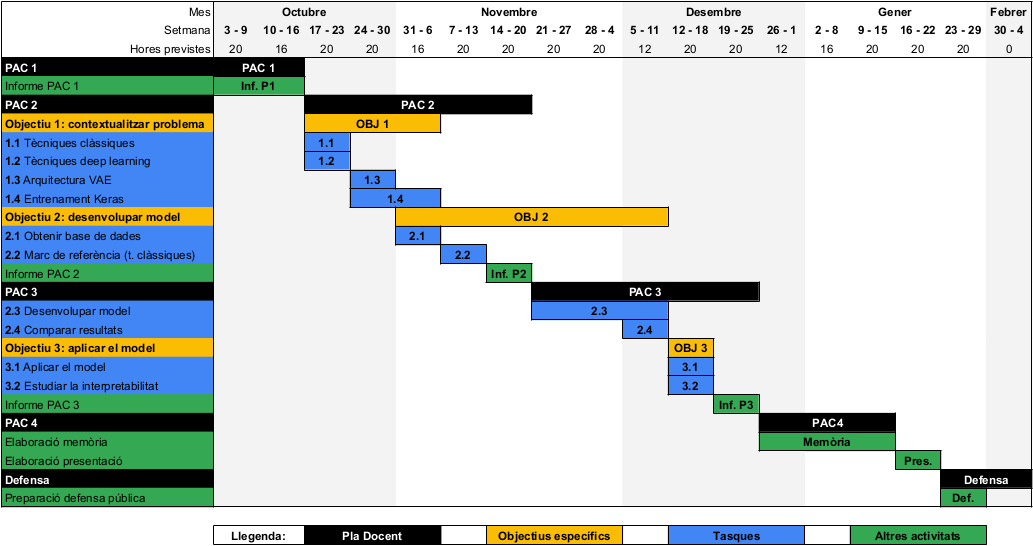
\includegraphics[width=\textheight]{TFM_calendari.png}
                \caption[Calendari: diagrama de Gantt]{Diagrama de Gantt:
                planificació dels objectius i tasques.}
                \label{f:gantt}
            \end{sidewaysfigure}

        \subsection{Fites:}
        \label{sec:fites}

            Les fites definides
            com a dates clau per planificar el treball
            es presenten a la \cref{t:fites}.

            \begin{table}[htbp]
                \small
                \centering
                \begin{tabular}{@{}ll@{}}
                    \toprule
                    \textbf{Data límit} & \textbf{Fita} \\ \midrule
                    17/10/2022 & Elaboració del pla de treball.\\
                               & Entrega de l'informe de la PAC 1.\\
                    28/10/2022 & Finalitzar la recerca bibliogràfica (marc teòric).\\
                    04/11/2022 & Data límit per a l'obtenció d'un conjunt de dades.\\
                               & Consecució de l'objectiu 1.\\
                    21/11/2022 & Entrega de l'informe de la PAC 2.\\
                    09/12/2022 & Consecució de l'objectiu 2.\\
                    16/12/2022 & Consecució de l'objectiu 3.\\
                    24/12/2022 & Entrega de l'informe de la PAC 3.\\
                    15/01/2023 & Entrega de la memòria i presentació.\\
                    23/01/2023 & Defensa pública\\ \bottomrule
                \end{tabular}
                \caption[Fites i dates clau]{Fites definides com a dates clau per planificar el treball.}
                \label{t:fites}
            \end{table}


    \section{Breu sumari de productes obtinguts}
        %No cal entrar en detall: la descripció detallada es farà a la resta de capítols.

        Com a resultat d'aquest \gls{tfm},
        s'han implementat diversos models de \textit{deep learning}
        basats en l'arquitectura \gls{ae}:
        \gls{vae}, \gls{dec}, \gls{vade}.
        Aquests models s'han compilat en un mòdul de Python,
        que es pot carregar fàcilment sense necessitat de re-escriure tot el codi.
        El mòdul s'ha fet públic a un repositori Github:
        \url{https://github.com/carlescn/MSc_bioinformatics_thesis}.

        S'ha obtingut també una serie de resultats
        d'aplicar aquests models i altres tècniques de \textit{clustering}
        sobre diversos conjunts de dades.
        Els resultats estàn formats per diverses mètriques de rendiment
        així com les assignacions de les observacions dels conjunts de dades
        als diversos clústers els resultats per cada mètode.
        Aquesta informació es pot fer servir en un estudi posterior,
        i també s'ha fet pública al mateix repositori.

    \section{Breu descripció dels altres capítols de la memòria}
        %Breu explicació dels continguts de cada capítol i la seva relació amb el projecte global.

    \paragraph{\Cref{c:state} \nameref{c:state}}
        En aquest primer capítol
        s'introdueixen les tècniques de \textit{clustering} clàssiques,
        el concepte d'\gls{fl},
        i les avantatges que poden suposar els models basats en xarxes neuronals profundes.

    \paragraph{\Cref{c:metodes} \nameref{c:metodes}}
        Aquí es presenta la base teòrica que sosté
        els models de \textit{deep clustering} escollits,
        així com algunes particularitats de la seva implementació.
        A continuació es detallen les mètriques
        utilitzades per avaluar el seu rendiment.

        Tot seguit
        es presenten els conjunts de dades utilitzats
        i s'explica detingudament la metodologia seguida
        per avaluar i comparar els diversos models.

        Finalment,
        es mencionen breument les eines informàtiques utilitzades
        per implementar els models de \textit{deep clustering}
        i avaluar els resultats.

    \paragraph{\Cref{c:resultats} \nameref{c:resultats}}
        En aquest capítol
        es presenten els resultats obtinguts
        i se'n fa un breu resum.
        La totalitat dels resultats
        es presenten en taules i figures als corresponents apèndixs.

    \paragraph{\Cref{c:discussio} \nameref{c:discussio}}
        Seguidament es discuteixen els resultats.
        Es discuteix els avantatges i inconvenients
        dels models implementats
        i es fa una breu valoració de la interpretabilitat del clústers obtinguts.

    \paragraph{\Cref{c:economic} \nameref{c:economic}}
        En aquest capítol es resumeix breument
        el petit cost econòmic que ha suposat
        el desenvolupament d'aquest \gls{tfm}.

    \paragraph{\Cref{c:conclusions} \nameref{c:conclusions}}
        Finalment,
        es presenta de manera sintetitzada les conclusions
        que s'han tret d'aquest \gls{tfm}
        i es fa una sèrie de propostes
        per futurs treballs,
        que no ha donat temps d'estudiar en el temps disponible.

    \glsunset{fl}

\chapter{Estat de l'art}
\label{c:state}
    %Estat de l'art del tema en qüestió.
    %Hauria d'acabar mostrant per què el treball és important i aporta alguna cosa, i amb les hipòtesis del treball.

    \section{Tècniques de \textit{clustering}}
    \label{s:state_cluster}

        Les tècniques de \textit{clustering} són un conjunt de tècniques estadístiques o d'aprenentatge automàtic no supervisat que es basen en agrupar les observacions en funció d'alguna mesura de la seva similitud, sense coneixement previ de l'estructura de les observacions o el nombre de grups que es pretén obtenir.

        L'objectiu d'aquestes tècniques és separar les dades en diversos grups que siguin internament homogenis (les observacions dins el mateix grup són similars entre ells) i tinguin característiques diferents a la resta de grups.

        Identificar aquests grups permet obtenir informació sobre l'estructura de les dades com la presència de patrons, i pot servir com a un punt de partida en l'exploració de les dades. Per exemple, aplicades a dades metabolòmiques, les tècniques de \textit{clustering} poden permetre identificar diferents tipus cel·lulars en funció de la seva expressió metabòlica \citep{Blekherman2011}.

        Existeix una gran varietat de tècniques de \textit{clustering} \citep{Karim2021, Min2018, Blekherman2011, Masood2015}. Encara que totes comparteixen un mateix objectiu, aborden el problema aplicant diferents criteris i per tant els grups que formen poden no coincidir. Algunes de les aproximacions més utilitzades històricament es basen en mètodes matemàtics i estadístics \citep{Masood2015}, com mètodes jeràrquics, mètodes basats en centroides, distribucions o densitats \citep{Karim2021}.

        \textbf{Mètodes jeràrquics:} es basen en crear clústers amb un ordre predeterminat, on els clústers de més baix nivell es combinen iterativament per crear clústers més grans. Això els dota d'una estructura jeràrquica que es pot presentar en forma de dendrograma, però implica que l'assignació de cada punt a un clúster és determinista. Aquests algoritmes no requereixen fixar prèviament un número de clústers, però són sensibles al soroll \citep{Karim2021}.

        \textbf{Mètodes basats en centroides:} (p. ex. \textit{k-means}) es basen assignar cada punt a un número predeterminat de grups i calcular els seus centroides. Després es canvia iterativament l'assignació de cada punt als diferents grups fins a minimitzar la suma de les distàncies de cada punt al centroide del seu grup. En general aconsegueixen un millor rendiment que els mètodes jeràrquics, però son incapaços de trobar grups no convexos \citep{Karim2021}.

        \textbf{Mètodes basats en distribucions:} (p. ex. model de barreja gaussiana (GMM)) es basen en modelar els grups en funció d'una barreja de distribucions probabilístiques. La seva base estadística permet inferir relacions entre les característiques de les dades, però requereix de fortes assumpcions sobre la distribució de les dades i tenen tendència a sobre-ajustament \citep{Karim2021}.

        \textbf{Mètodes basats en densitats:} (p. ex. DBSCAN) defineixen els clústers com àrees amb major densitat comparats amb la resta de les dades. Els punts en regions més disperses es consideren fronteres o soroll. El punt negatiu d'aquests mètodes és precisament que requereixen d'una disminució de la densitat per detectar les fronteres dels clústers i són poc eficaces en separar grups contigus \citep{Karim2021}.

    \section{Reducció de la dimensionalitat}
    \label{s:state_reduccio}

        Un dels problemes que apareix habitualment al analitzar dades bioinformàtiques és la seva elevada dimensionalitat, característica que fa que les tècniques de \textit{clustering} clàssiques no funcionin bé \citep{Masood2015, Karim2021}. Per combatre aquest problema, una solució és aplicar tècniques de reducció de la dimensionalitat i posteriorment aplicar les tècniques de \textit{clustering} sobre les dades transformades \citep{Min2018, Masood2015}.

        La reducció de la dimensionalitat s'aconsegueix mitjançant tècniques d'\gls{fl}. L'objectiu d'aquestes tècniques és representar les dades originals en un espai dimensional inferior, aplicant una transformació que retingui el màxim d'informació. L'espai reduït resultant s'anomena \gls{cr} i les seves dimensions \gls{lf}.

        Històricament s'han utilitzat tècniques matemàtiques per realitzar \gls{fl}, que poden ser transformacions lineals (anàlisi de components principals) o no lineals (mètodes kernel o tècniques espectrals). Posteriorment s'apliquen les tècniques de clustering sobre les \gls{lf}.

        Una limitació dels mètodes lineals és que no són capaços de retenir informació sobre relacions no lineals en les dades, el que provoca una reducció de la \gls{qc}. Les tècniques no lineals són més adequades \citep{Karim2021}.

    \section{Tècniques de \textit{deep clustering}}
    \label{s:state_deep}

        Les xarxes neuronals profundes possibiliten aplicar tècniques de \gls{fl} més eficients que les descrites a la secció anterior, aplicant mètodes no lineals complexes que permeten capturar \gls{lf} més rellevants. En particular, la funció de transformació es pot optimitzar mitjançant l'aprenentatge dels paràmetres de la xarxa, el que permet extreure \gls{lf} òptimes per obtenir una bona \gls{qc} \citep{Karim2021}.

        La seva recent popularització ha fet possible desenvolupar un gran nombre de tècniques de \textit{clustering} basades en \textit{deep learning}, anomenades en conjunt tècniques de \textit{deep clustering}. Es poden dividir en dos grans grups: mètodes de dos passos, que es basen en utilitzar tècniques de \gls{fl} i aplicar mètodes de \textit{clustering} convencionals sobre les \gls{lf}; i mètodes d'un sol pas que desenvolupen un model de \textit{clustering} sobre les dades originals \citep{Karim2021}.

        A la literatura s'ha descrit una gran varietat de mètodes basats en diferents arquitectures neuronals (\gls{mlp}, \gls{cnn}, \gls{dbn}, \gls{gan}, \gls{ae}). A \url{https://github.com/rezacsedu/Deep-learning-for-clustering-in-bioinformatics} \citep{Karim2021} es pot trobar un llistat amb enllaços als articles originals.

        La majoria d'aproximacions actuals utilitzen una arquitectura basada en un \gls{ae} \citep{Karim2021}, donat que és capaç d'obtenir \gls{lf} eficients per realitzar \textit{clustering}.


    \section{Autoencoder}
    \label{s:state_ae}

        \begin{figure}
            \centering
            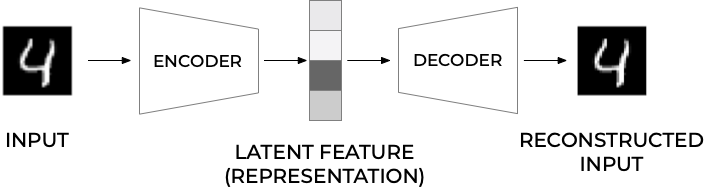
\includegraphics[width=\textwidth]{michelucci2022_autoencoder.png}
            \caption[Esquema del model Autoencoder]{
                Esquema del model \gls{ae}.
                Font: Michelucci, 2022 \citep{Michelucci2022}
            }
            \label{f:ae_michelucci}
        \end{figure}

        L'arquitectura \gls{ae} està formada per dues parts: un codificador i un descodificador. La funció del codificador és representar l'entrada en un espai dimensional reduït, sovint un vector, anomenat codi. La funció del descodificador és reconstruir l'entrada original a partir del codi. A la \cref{f:ae_michelucci} es mostra esquema de l'arquitectura \gls{ae}.

        Optimitzant els paràmetres d'ambdues parts conjuntament durant l'entrenament de la xarxa es busca aconseguir que el codificador sigui capaç de comprimir la entrada mantenint el màxim d'informació. Aplicant la idea de \gls{fl}, el codi esdevé la \gls{cr}.

        Per aconseguir un \textit{clustering} eficaç, no és suficient amb aquesta optimització ja que si no s'aplica cap restricció a la \gls{cr} podria donar lloc a \gls{lf} que no permeten una bona \gls{qc}. Per resoldre aquest problema es defineixen dos tipus de funció de cost, que s'optimitzen conjuntament durant l'entrenament \citep{Min2018}:
        \begin{itemize}
            \item La \textbf{funció de cost auxiliar}, que depèn de la capacitat del codificador d'obtenir una \gls{cr} eficient que permeti que el descodificador sigui capaç de regenerar l'entrada. Garanteix obtenir \gls{lf} rellevants.
            \item La \textbf{funció de cost de \textit{clustering}}, que depèn de l'algoritme de \textit{clustering} i de que les \gls{lf} obtingudes siguin adequades per realitzar \textit{clustering}. Assegura obtenir una bona \gls{qc}.
        \end{itemize}

        L'aproximació més bàsica de l'arquitectura \gls{ae} es pot construir utilitzant \glspl{mlp} simètrics pel codificador i descodificador. Encara que és fàcil d'implementar, el model generat conté un gran nombre d'hiperparàmetres i esdevé difícil d'optimitzar i balancejar les dues funcions de cost \citep{Karim2021}. A més, no s'aplica cap restricció a la funció de representació i per tant no garanteix obtenir una bona \gls{qc}.

        A la literatura s'han descrit diferents aproximacions a la idea del \gls{ae}, que prenen com a base altres arquitectures. Algunes d'aquestes aproximacions permeten aconseguir un model generatiu, que és capaç de generar dades similars a les d'entrenament. Alguns d'aquestes aproximacions són:

        \textbf{\Gls{cae}:} l'arquitectura \gls{ae} estàndard no dona bons resultats per trobar patrons en imatges (dades amb invariança espacial). Per combatre-ho, es poden combinar amb \gls{cnn} utilitzant convolucions al codificador del \gls{ae} (i les corresponents desconvolucions al descodificador), on els filtres de la \gls{cnn} són un paràmetre que es pot optimitzar (en lloc de construir-los a mà com en una \gls{cnn} estàndard).

        \textbf{\Gls{vae}:} aquesta aproximació es basa en mètodes Bayesians, el que li atorga certa robustesa estadística que no tenen altres arquitectures. Es tracten les dades com a mostres d'una distribució desconeguda i s'aplica una restricció al codificador perquè les representi com una barreja de distribucions conegudes (per exemple, gaussianes). Els paràmetres que aprèn la xarxa són els paràmetres de les distribucions (mitjana i variància). El descodificador reconstrueix les mostres originals, el que permet generar mostres aleatòries semblants a la distribució original desconeguda. S'explica amb més detall a la \cref{s:metodes_vae}.

        \textbf{\Gls{lstmae}:} de manera similar al cas del \gls{cae}, l'arquitectura \gls{ae} estàndard no funciona bé amb dades seqüencials, però es pot combinar amb l'arquitectura \gls{lstm}. El codificador es forma combinant capes \gls{lstm}, on la última capa codifica un vector que representa l'entrada de la xarxa. El descodificador, també format per capes \gls{lstm}, pren aquest vector (replicat per adaptar-lo a l'entrada de la primera capa \gls{lstm}) i reconstrueix l'entrada original.

        \textbf{\Gls{aae}:} aquesta aproximació pren la idea del discriminador de la arquitectura \gls{gan} i la introdueix al \gls{ae}. L'objectiu és representar les dades originals com una barreja de distribucions conegudes, de manera similar al \gls{vae}. En aquest cas la xarxa està formada per tres parts: el codificador, que redueix l'entrada a un codi, el descodificador, que reconstrueix la entrada a partir del codi, i un discriminador. El discriminador intenta discriminar entre els codis generats i punts mostrejats aleatòriament de la distribució escollida. El resultat és que els codis generats acaben aproximant-se a aquesta distribució \citep{Makhzani2015}.

        \textbf{\Gls{dae}:} aquesta tècnica entrena el \gls{ae} introduint soroll a l'entrada del codificador i reconstruint les dades originals amb el descodificador. Això permet aprendre una representació més robusta de les dades i també la reconstrucció de les dades originals a partir d'unes dades parcialment corrompudes.

        \textbf{\Gls{sae}:} diversos \gls{ae} es poden apilar per aconseguir representacions més comprimides de les dades d'entrada. S'entrena un primer \gls{ae} per comprimir i reconstruir les dades d'entrada i es pren el codi comprimit. Aquest codi es pren com l'entrada d'un segon \gls{ae}, que s'entrena per comprimir i reconstruir el codi. Aquest procés es repeteix fins a aconseguir el nombre de capes desitjat. Finalment, s'ordenen les capes codificadores i descodificadores de cada \gls{ae} seqüencialment, formant un \gls{sae}, i s'entrena una última vegada el model sencer per ajustar tots els pesos. D'aquesta manera s'obté un model capaç de codificar les dades en un espai dimensional més reduït.

        En aquest \gls{tfm}, es desenvoluparà un model de \textit{deep clustering} utilitzant una arquitectura \gls{vae}, ja que les seves característiques el fan un model interessant. El model probabilístic li atorga certa robustesa estadística que pot ser útil al extreure conclusions del resultats obtinguts. Alhora, la capacitat generativa pot permetre generar mostres artificials semblants a les originals, el que podria servir com a tècnica d'augment de dades (\textit{data augmentation}).


\chapter{Materials i mètodes}
\label{c:metodes}
    %En aquests apartats, cal descriure:
    %\begin{itemize}
    %    \item Els aspectes més rellevant del disseny i desenvolupament del treball.
    %    \item La metodologia triada per a fer aquest desenvolupament, descrivint les alternatives possibles, les decisions preses, i els criteris utilitzats per prendre aquestes decisions.
    %    \item Els productes obtinguts.
    %\end{itemize}
    %\textbf{L’estructuració dels capítols pot variar segons el tipus de treball.}

    \section{Tècniques de \textit{clustering} clàssiques}
    \label{s:metodes_classic}

    A continuació s'expliquen de manera molt sintetizada
    les tres tècniques de \textit{clustering} clàsiques utilitzades com a referència
    per comparar amb les tècniques de \textit{deep clustering}.

    \paragraph{\Gls{kmeans}}
        El mètode \gls{kmeans}
        és un algoritme de \textit{clústering}
        que minimitza les distàncies entre cada objecte
        al centroide del seu clúster.
        La distància es sol calcular utilitzant la \gls{sse}.

        L'algoritme consta de tres passos:
        s'escull un número $k$ de clústers
        i $k$ punts en l'espai,
        que seran els centroides inicials.
        S'assigna cada punt al clúster que minimitza la distància al seu centroide.
        S'actualitza la posició dels centroides
        calculant la posició mitjana dels punts associats a cada clúster.
        Finalment es repeteixen els dos últims passos
        fins que els centroides deixen de moure's.

        La principal avantatge d'aquest mètode és que és un mètode senzill i ràpid,
        però requereix escollir un valor de $k$ arbitrari
        i no garanteix convergir en un mínim global.

    \paragraph{\Gls{gmm}}
        El model \gls{gmm}
        és un model probabilístic que assumeix que les observacions
        s'han generat d'una barreja finita de distribucions normals (gaussianes).

        Cada distribució està caracteritzada per una mitjana
        una covariància i una probabilitat $\pi$,
        que defineix la mida de la distribució.
        La suma de les probabilitats $\pi$ de totes les distribucions
        ha de resultar sempre 1.

        Així, fixant un nombre de clústers $k$
        i utilitzant mètodes Bayesians
        es poden calcular els paràmetres de les distribucions
        que maximitzen la probabilitat de les mostres observades.
        No es considera necessari entrar en detall dels càlculs matemàtics.

        Una característica d'aquest model
        és que no assigna un clúster determinat a cada observació,
        si no una probabilitat de pertànyer a cada clúster.

        El model resultant és un model generatiu:
        coneixent els paràmetres de les distribucions,
        es poden calcular mostrejar nous punts
        que haurien de distribuir-se com les variables estudiada.

        Igual que el mètode \gls{kmeans},
        presenta l'inconvenient que és necessari escollir prèviament
        un valor de $k$ arbitrari.

    \paragraph{\Gls{aglo}}
        L'algoritme de \textit{clustering} aglomeratiu
        es basa en construir una jerarquia
        de grups en funció de la seva similaritat.

        El procés s'inicia assignant un grup unitari a cada observació,
        A continuació es calcula la distància entre cada parell de grups
        i s'uneixen els dos que minimitzen aquest valor.
        Aquest procés es repeteix fins que només queda un grup global.

        Per calcular la distància entre punts
        es poden utilitzar diferents mètriques,
        com ara la distància Euclidiana, la distància de Manhattan, etc.
        La distància entre grups també es pot calcular segons diferents criteris:
        agrupament màxim (la distància entre dos grups es determina per la distància màxima entre dos punts),
        agrupament mínim (es determina per la mínima distància entre dos punts), etc.

        Aquest mètode presenta l'avantatge de no requerir seleccionar un número de clústers arbitrari.
        A més, el conjunts resultants es poden representar en un dendrograma
        que representa gràficament la similitud entre els punts i entre grups.

        Un inconvenient és que són sensibles al soroll:
        una petita variació en les dades pot desembocar en grups completament diferents.

    \section{Models de \textit{deep clustering}}
    \label{s:metodes_dc}

    En aquest \gls{tfm}
    es pretén implementar diversos model de \textit{deep clustering} en dades metabòliques.
    Com s'ha descrit a les \cref{s:state_deep,s:state_ae},
    existeix una gran varietat d'arquitectures de xarxes neuronals descrites a la literatura.
    Intentar estudiar totes les possibilitats seria inabastable donat el temps disponible,
    pel que ha sigut necessari acotar l'estudi a una única arquitectura.
    S'ha decidit implementar algunes aproximacions basada en \gls{ae}.

    A continuació es fa una breu presentació dels models
    \gls{dec} \citep{Xie2015}, \gls{vae} \citep{Kingma2014,Kingma2019} i \gls{vade} \citep{Jiang2020}
    basada en les referències indicades al costat de cada model.
    No s'entrarà en profunditat en les explicacions matemàtiques.
    Per una explicació més detallada es recomana llegir les fonts originals.


    \subsection{Deep embedded clustering}
    \label{s:metodes_dec}

        \begin{figure}
            \centering
            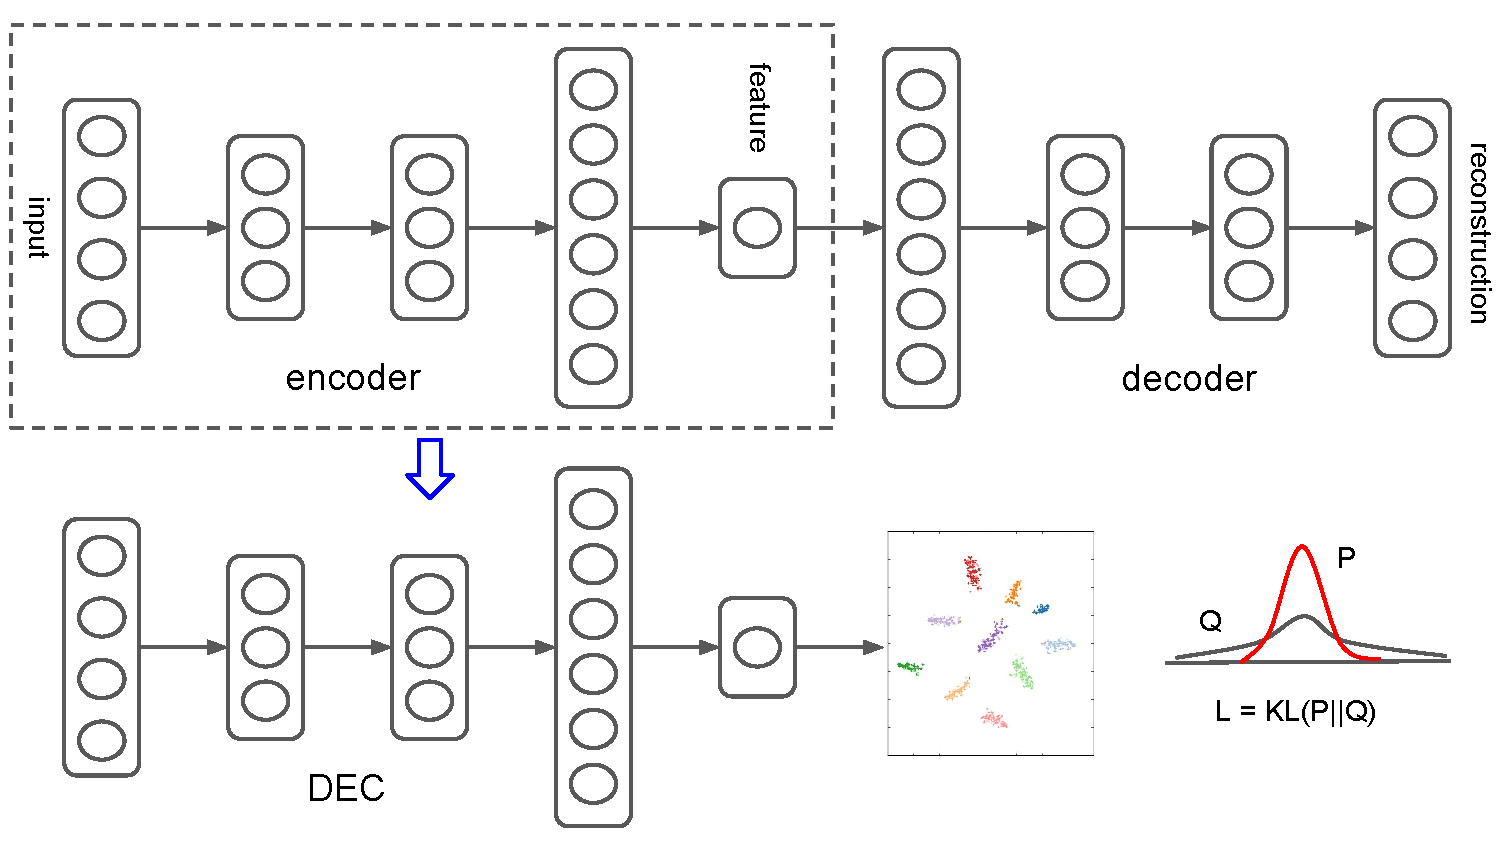
\includegraphics[width=0.7\textwidth]{xie2015_dec.pdf}
            \caption[Arquitectura del model DEC mantenint]{
                Esquema de l'arquitectura del model \gls{dec}.
                Font: Xie \textit{et. al.}, 2015 \citep{Xie2015}
            }
            \label{f:dec_xie2015}
        \end{figure}

        El model \gls{dec} es basa en un \gls{ae}
        al que, després de la fase d'entrenament habitual,
        s'elimina el descodificador i
        es substitueix per una nova xarxa neuronal,
        la sortida de la qual es pot tractar
        com un vector de probabilitats d'assignacions a clústers,
        com s'il·lustra a la \cref{f:dec_xie2015}.

        Primerament,
        s'entrena un model \gls{ae}
        aplicant únicament una \textbf{funció de cost de reconstrucció},
        que busca minimitzar la distància entre la sortida del descodificador
        i l'entrada original del codificador.
        Poden utilitzar-se diferents funcions,
        com ara la \gls{sse},
        la \gls{mse}
        o la entropia creuada.
        A la \cref{s:metodes_vae} s'entra en més detall
        sobre la funció escollida i com es calcula.

        Un cop entrenat,
        s'obté un model amb un codificador
        és capaç de representar les dades d'entrada $\mathbf{x}$
        en un espai latent $\mathbf{z}$,
        i un descodificador capaç de generar mostres simulades
        a partir de $\mathbf{z}$.
        És a dir, el model ha après unes \gls{lf} rellevants de les dades
        que permeten obtenir una \gls{cr} eficient.

        El següent pas és aplicar una tècnica de \textit{clustering}
        sobre les representacions de l'espai latent $\mathbf{z}$.
        Per aconseguir-ho,
        es construeix un model de \textit{clustering}
        basat en una nova capa neuronal.
        Els pesos de cada neurona d'aquesta capa
        corresponen a la posició del centroide d'un clúster.
        Una limitació d'aquesta tècnica és que requereix
        establir el nombre $k$ de clústers prèviament.

        La capa pren com entrada un punt de $\mathbf{z}$
        i calcula la distància del punt a cada centroide.
        La sortida de la capa és un vector de longitud $k$ que suma 1,
        on cada valor representa la probabilitat d'assignació del punt a cada clúster.
        Aquesta assignació s'interpreta com una distribució $Q$.

        A continuació es defineix una nova funció de cost,
        la \textbf{funció de cost de \textit{clustering}},
        com la distància \gls{kl} entre la distribució $Q$
        i una distribució auxiliar $P$.
        Escollint una distribució auxiliar adequada,
        al minimitzar aquesta distància
        s'aconsegueix millorar la \gls{qc}:
        es minimitza la distància de cada punt al seu centroide
        alhora que es maximitza la distància a la resta de centroides.

        La distribució auxiliar $P$ es calcula
        a partir de $Q$:
        \begin{equation}
            \label{eq:clustering_aux}
            p_{ij} =
            \frac {q_{ij}^2 / f_j}
            {\sum_j' q_{ij}^2 / f_j'}
        \end{equation}

        on $p_{ij}$ i $q_{ij}$ són respectivament la probabilitat
        de $P$ i $Q$ per la observació $i$ i el clúster $j$,
        i $f_j$ és la freqüència del clúster $j$.

        El model \gls{dec} es construeix prenent només el codificador
        del \gls{ae} entrenat prèviament,
        i afegint la capa de \textit{clustering}.
        Abans d'iniciar l'entrenament del nou model,
        és necessari establir uns paràmetres inicials
        (els pesos i biaixos de les neurones de la capa de \textit{clustering}).

        Es passen les dades d'entrenament pel codificador
        per obtenir les seves representacions en l'espai $\mathbf{z}$.
        Seguidament s'aplica un mètode de \textit{clustering}
        (l'autor proposa \textit{K-means})
        i es pren la posició dels centroides.

        Finalment, s'entrena la xarxa utilitzant el descens de gradients estocàstic
        optimitzant únicament per la funció de cost de \textit{clustering}.
        El model aprendrà una nova representació en l'espai latent $\mathbf{z}$,
        juntament amb una posició òptima dels centroides que defineixen cada clúster,
        que en conjunt optimitzin la \gls{qc}.
        És important mencionar que al descartar el descodificador
        i no utilitzar la funció de cost de reconstrucció,
        no es pot assegurar que el model mantingui les \gls{lf} apreses.

        Alternativament,
        es pot construir un model alternatiu
        que sí manté el descodificador \citep{Min2018} (\cref{f:dec_min2018}).
        En aquest cas el model s'entrena aplicant conjuntament les dues funcions de cost
        (de reconstrucció i de \textit{clustering}).
        D'aquesta manera s'assegura mantenir mantenir unes \gls{lf} rellevants a la \gls{cr}.

        \begin{figure}
            \centering
            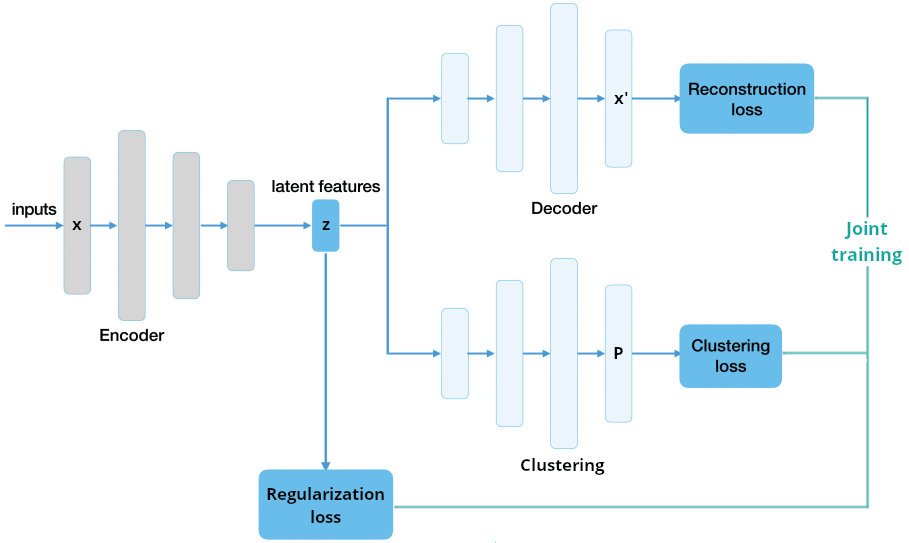
\includegraphics[width=\textwidth]{min2018_losses.png}
            \caption[Alternativa al DEC mantenint descodificador]{
                Esquema del model \gls{dec} alternatiu,
                que manté el descodificador
                i s'entrena aplicant conjuntament les funcions de cost
                de reconstrucció i de \textit{clustering}.
                Font: Min \textit{et. al.}, 2018 \citep{Min2018}
            }
            \label{f:dec_min2018}
        \end{figure}

    \subsection{Variational Autoencoder}
    \label{s:metodes_vae}

        Com s'ha mencionat a la \cref{s:state_ae},
        l'arquitectura \gls{vae} és una implementació específica de \gls{ae}
        basada en mètodes Bayesians.
        Això li atorga al model certa robustesa estadística
        que no trobem en altres arquitectures.
        A més,
        la \gls{cr} apresa permet la generació de mostres artificials
        similars a les dades d'entrenament.
        Això últim pot resultar útil com a tècnica d'augment de dades.

        En l'arquitectura \gls{ae},
        el codificador aprèn una representació de l'entrada $\mathbf{x}$
        en un espai dimensional reduït $\mathbf{z}$
        aplicant una transformació no lineal.
        Des de la perspectiva de \gls{fl},
        aquest espai reduït es correspon amb la \gls{cr}.
        El descodificador aprèn a reconstruir $\mathbf{x}$ a partir de $\mathbf{z}$
        aplicant una segona transformació no lineal.
        L'entrenament de les dues parts conjuntament
        aconsegueix que les \gls{lf} siguin una bona representació de les dades originals.

        En l'aproximació que pren el \gls{vae},
        s'assumeix que l'entrada $\mathbf{x}$ és un conjunt d'observacions de variables aleatòries,
        que provenen d'un procés desconegut
        amb una distribució $p^*(\mathbf{x})$.
        Aquesta distribució és desconeguda,
        de manera que intentem aproximar-la amb un model $p_\theta(\mathbf{x})$,
        on $\theta$ són els paràmetres del model.

        L'espai $\mathbf{z}$ es considera un conjunt de variables latents del model
        que segueixen una distribució $p_\theta(\mathbf{z})$.
        Les variables latents són variables que estan presents al model però no observem en les dades.
        Es pot fixar que $p_\theta(\mathbf{z})$ sigui una distribució fàcil de computar,
        per exemple una barreja de gaussianes.

        Sota aquesta premissa,
        el model a inferir és sobre una distribució conjunta $p_\theta(\mathbf{x,z})$
        de les variables observades i latents.
        L'objectiu del codificador és aprendre els paràmetres $\theta$
        de la distribució $p_\theta(\mathbf{z|x})$
        (la distribució posterior de $\mathbf{z}$ condicionada a $\mathbf{x}$).
        De la mateixa manera,
        l'objectiu del descodificador és aprendre els paràmetres $\theta$
        de la distribució $p_\theta(\mathbf{x|z})$.
        A la \cref{f:vae_kingma} s'il·lustra
        com el model relaciona els espais $\mathbf{x}$ i $\mathbf{z}$.

        \begin{figure}
            \centering
            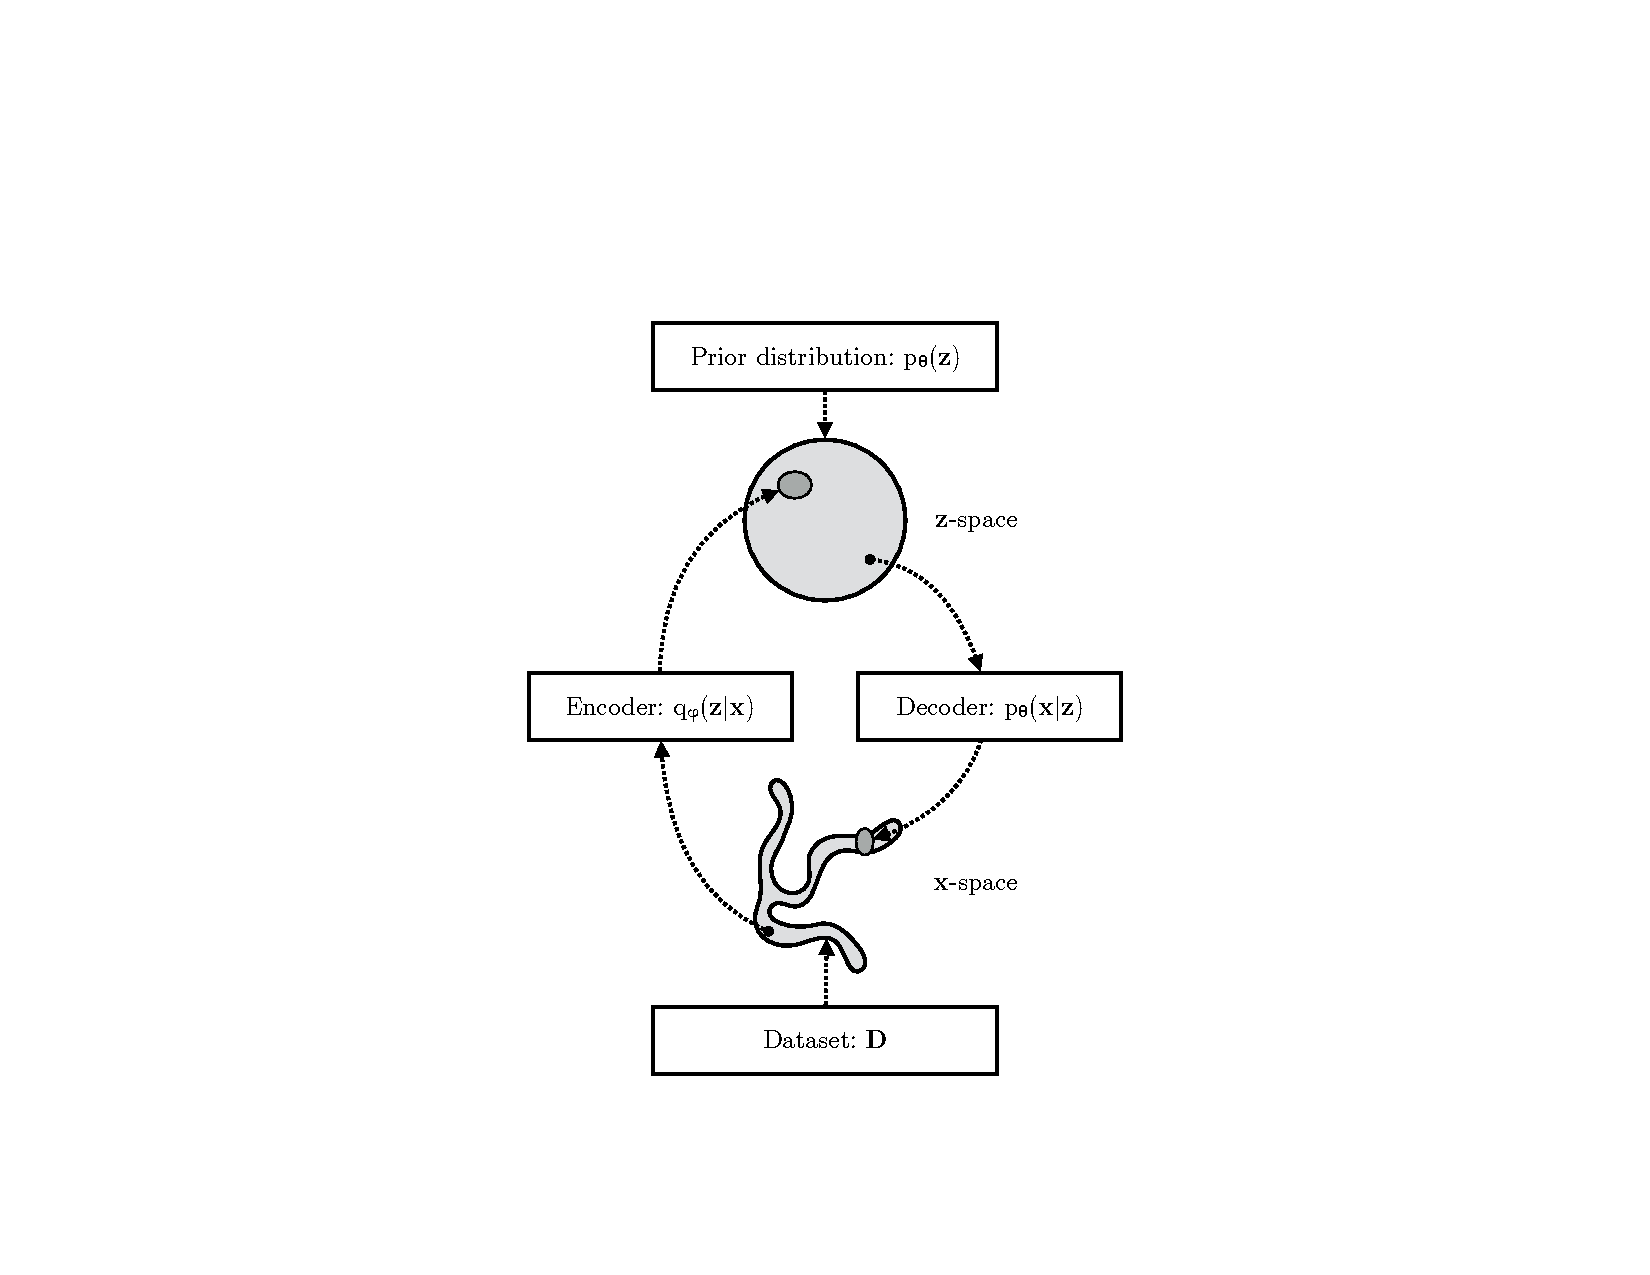
\includegraphics[width=0.5\textwidth]{kingma2019_vae.pdf}
            \caption[\textit{Variational autoencoder}: model probabilístic]{
                Esquema del model \gls{vae}.
                Les dades observades $\mathbf{D}$ (\textit{dataset})
                són una mostra d'unes variables de l'espai $\mathbf{x}$,
                que segueix una distribució intractable.
                L'espai latent $\mathbf{z}$ s'escull que segueixi
                una distribució $p_\phi(\mathbf{z})$ fàcil de computar.
                El codificador (\textit{encoder})
                troba la distribució condicional de $\mathbf{z}$ donada $\mathbf{x}$,
                aconseguint una representació de les mostres a l'espai latent.
                El decodificador (\textit{decoder})
                troba la distribució condicional de $\mathbf{x}$ donada $\mathbf{z}$,
                aconseguint la reconstrucció de les dades a partir de l'espai latent.
                Font: Kingma and Welling, 2019 \citep{Kingma2019}
            }
            \label{f:vae_kingma}
        \end{figure}

    \subsection{Optimització dels paràmetres}
    \label{s:vae_optimitzacio}

        El codificador pretén aprendre els paràmetres $\theta$ òptims
        de la distribució $p_\theta(\mathbf{z|x})$,
        que està condicionada per la distribució marginal $p_\theta(\mathbf{x})$
        segons la equació:
        \begin{equation}
        \label{eq:cond_p_z_on_x}
            p_\theta(\mathbf{z|x}) =
            \frac {p_\theta(\mathbf{x,z})}
                  {p_\theta(\mathbf{x})}
        \end{equation}

        Aquesta distribució marginal en el model bé donada per:
        \begin{equation}
        \label{eq:marginal_p_x}
            p_\theta(\mathbf{x}) = \int p_\theta(\mathbf{x, z}) d\mathbf{z}
        \end{equation}

        La integral en la \cref{eq:marginal_p_x} provoca que
        la distribució marginal $p_\theta(\mathbf{x})$ no tingui un estimador eficient
        i sigui intractable computacionalment.
        Això provoca que no es pugui diferenciar respecte als paràmetres $\theta$
        i optimitzar-la pel mètode del descens de gradients.
        En conseqüència,
        tampoc es poden optimitzar els paràmetres de la distribució $p_\theta(\mathbf{z|x})$.

        En el seu lloc,
        es pot inferir un model $q_\phi(\mathbf{z|x})$
        que aproximi la distribució intractable $p_\theta(\mathbf{z|x})$,
        on els paràmetres $\phi$ s'aprenen a través de la optimització
        dels pesos i biaixos de la xarxa neuronal.

        La diferència entre aquestes dues distribucions
        es pot calcular mitjançant la divergència de \gls{kl}:
        $D_{KL} ( q_\phi(\mathbf{z|x}) \| p_\theta(\mathbf{z|x}) )$.
        L'objectiu és minimitzar aquesta divergència,
        però no és possible calcular-la directament
        donada la intractabilitat de $p_\theta(\mathbf{z|x})$.

        Aquesta divergència es relaciona amb la distribució marginal
        segons la següent igualtat:
        \begin{equation}
            \label{eq:kl}
            \log p_\theta(\mathbf{x}) =
            \mathcal{L}_{\theta,\phi}(\mathbf{x}) +
            D_{KL} (
            q_\phi(\mathbf{z|x}) \|
            p_\theta(\mathbf{z|x})
            )
        \end{equation}

        Per tant, es pot minimitzar la divergència maximitzant el terme $\mathcal{L}_{\theta,\phi}(\mathbf{x})$.
        Aquest terme s'anomena \gls{elbo}
        ja que la divergència \gls{kl} és sempre no negativa i
        per tant \gls{elbo} és el límit inferior de $\log p_\theta(\mathbf{x})$
        (evidència de $\mathbf{x}$):
        \begin{equation}
            \label{eq:lim_inf}
            \log p_\theta(\mathbf{x}) \ge
            \mathcal{L}_{\theta,\phi}(\mathbf{x})
        \end{equation}

        El terme \gls{elbo} es calcula segons la següent equació:
        \begin{equation}
        \label{eq:elbo}
            \mathcal{L}_{\theta,\phi}(\mathbf{x}) =
            \mathbb{E}_{q_\phi(\mathbf{z|x})}
                [ \log p_\theta(\mathbf{x|z}) ] -
            \mathbb{E}_{q_\phi(\mathbf{z|x})} \left[
                \log \frac {q_\phi(\mathbf{z|x})}
                           {p_\theta(\mathbf{z})}
            \right]
        \end{equation}

        La maximització del \gls{elbo} implica:
        \begin{itemize}
            \item Maximitzar el primer terme de la equació,
            la esperança de $\log p_\theta(\mathbf{x|z})$,
            que es correspon amb optimitzar els paràmetres del descodificador.
            És a dir, s'aconsegueix una millor reconstrucció.

            \item Minimitzar el segon terme,
            la esperança de $\log ( q_\phi(\mathbf{z|x}) / p_\theta(\mathbf{z}) )$,
            que és la divergència \gls{kl} entre
            la distribució inferida pel codificador $q_\phi(\mathbf{z|x})$
            i la distribució $p_\theta(\mathbf{z})$ fixada de l'espai latent.
            És a dir, s'aconsegueix millorar la representació obtinguda pel codificador.
        \end{itemize}

    \subsection{Descens de gradients}
    \label{s:vae_gradients}

        Per optimitzar els paràmetres de la xarxa neuronal
        de tal manera que es maximitzi el \gls{elbo},
        s'utilitza el descens de gradients.
        Per tant, cal calcular els gradients del \gls{elbo}
        amb respecte als paràmetres $\theta$ i $\phi$.

        El \gls{elbo} es pot reformular de la següent manera,
        el que facilitarà el càlcul dels gradients:
        \begin{equation}
        \label{eq:elbo_2}
            \mathcal{L}_{\theta,\phi}(\mathbf{x}) =
            \mathbb{E}_{q_\phi(\mathbf{z|x})} [
                \log p_\theta(\mathbf{x,z}) -
                \log q_\phi(\mathbf{z|x})
            ]
        \end{equation}

        I els gradients es calculen segons:
        \begin{gather}
        \label{eq:gradient_theta}
            \nabla_\theta \mathcal{L}_{\theta,\phi}(\mathbf{x}) =
            \nabla_\theta \mathbb{E}_{q_\phi(\mathbf{z|x})} [
            \log p_\theta(\mathbf{x,z}) -
            \log q_\phi(\mathbf{z|x})
            ]
        \\
        \label{eq:gradient_phi}
            \nabla_\phi \mathcal{L}_{\theta,\phi}(\mathbf{x}) =
            \nabla_\phi \mathbb{E}_{q_\phi(\mathbf{z|x})} [
            \log p_\theta(\mathbf{x,z}) -
            \log q_\phi(\mathbf{z|x})
            ]
        \end{gather}

        Per la regla de la integral de Leibniz, el gradient en la \cref{eq:gradient_theta} es pot moure a dins de la esperança i això permet la seva computació. Però el mateix no és possible en la \cref{eq:gradient_phi}, ja que l'esperança està en funció de $\phi$.

        Per resoldre aquest problema es planteja la següent solució:
        reparametritzar la variable $\mathbf{z} \sim q_\theta(\mathbf{z|x})$
        com una funció d'una altra variable aleatòria $\epsilon$, donades $\mathbf{x}$ i $\phi$:
        \begin{gather}
        \label{eq:epsilon}
            \epsilon \sim p(\epsilon) \\
        \label{eq:z_reparam}
            \mathbf{z} = g(\phi, \mathbf{x}, \epsilon)
        \end{gather}

        on la funció $g(\cdot)$ és una transformació determinista.
        Aquesta reparametrització s'il·lustra a la \cref{f:reparametritzacio}.
        Llavors, el \gls{elbo} es pot reescriure
        en funció de $\mathbb{E}_{p(\epsilon)}$
        en lloc de $\mathbb{E}_{q_\phi(\mathbf{z|x})}$,
        de manera que ``s'externalitza'' la aleatorietat de la variable $\mathbf{z}$
        a la nova variable $\epsilon$.
        La nova forma del gradient del \gls{elbo} en respecte a $\phi$ és:
        \begin{equation}
        \label{eq:gradient_phi_reparam}
            \nabla_\phi \mathcal{L}_{\theta,\phi}(\mathbf{x}) =
            \nabla_\phi \mathbb{E}_{p(\epsilon)} [
                \log p_\theta(\mathbf{x,z}) -
                \log q_\phi(\mathbf{z|x})
            ]
        \end{equation}

        Després d'aquesta reparametrització,
        es poden calcular els gradients del \gls{elbo}
        respecte als paràmetres $\phi$ i $\theta$,
        i així optimitzar-los mitjançant el descens de gradients.

        \begin{figure}
            \centering
            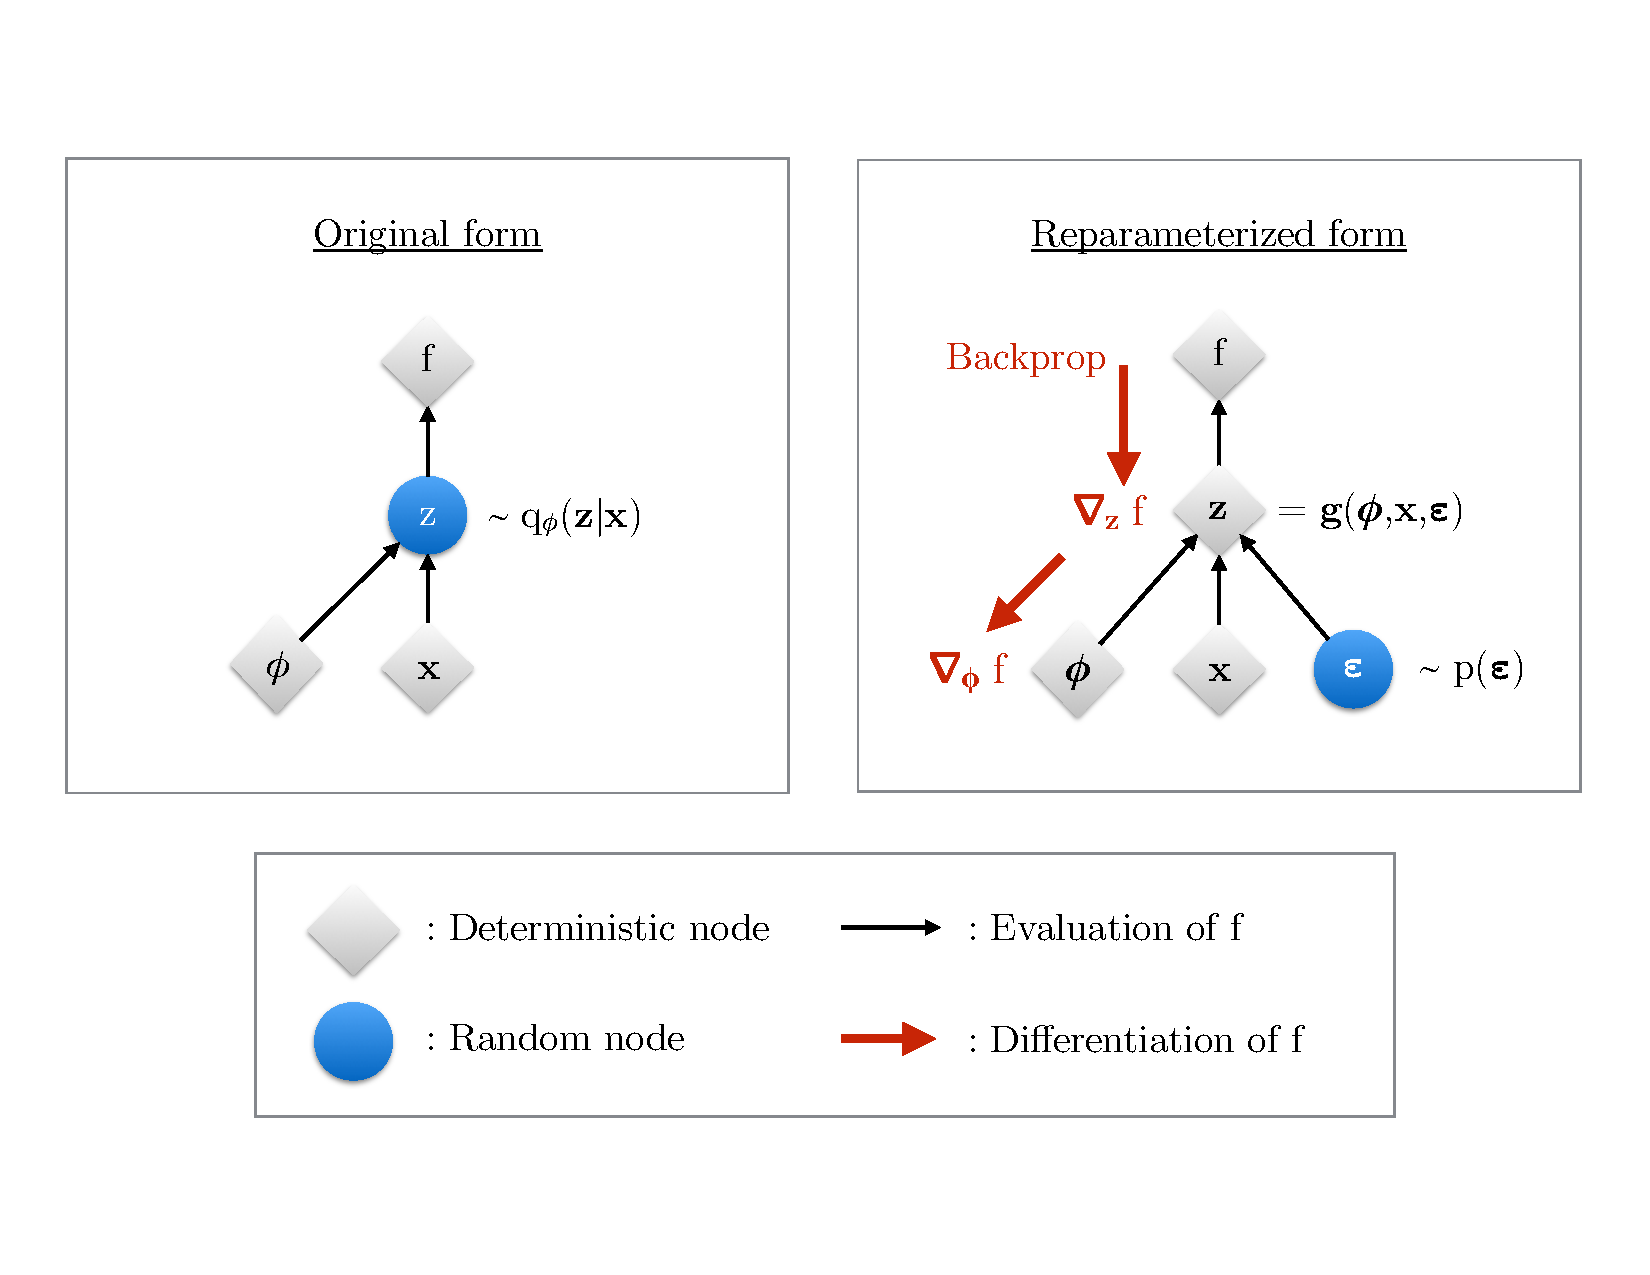
\includegraphics[width=0.7\textwidth]{kingma2019_reparam.pdf}
            \caption[Reparametrització de $\mathbf{z}$]{
                Il·lustració de la reparametrització de $\mathbf{z}$.
                Per optimitzar els paràmetres $\theta$
                es necessita calcular els gradients de la funció d'optimització $f$
                amb respecte a $\theta$.
                En la figura de l'esquerra (forma original)
                no es pot diferenciar $f$ amb respecte a $\theta$
                perquè no es poden propagar endarrere els gradients
                a través de la variable aleatoria $\mathbf{z}$.
                Després de la reparametrització (figura de la dreta),
                la aleatorietat queda ``externalitzada'' a la variable $\epsilon$,
                i $\mathbf{z}$ depèn d'una funció $g(\cdot)$ determinista.
                Aquesta configuració sí permet propagar endarrere els gradients.
                Font: Kingma and Welling, 2019 \citep{Kingma2019}
            }
            \label{f:reparametritzacio}
        \end{figure}

    \subsection{Implementació del model}
    \label{s:vae_implementacio}

        Un cop presentada la base teòrica,
        a continuació es resumeix com s'ha implementat el model \gls{vae}
        que s'ha construït en aquest \gls{tfm}.
        S'ha escollit que la variable latent $\mathbf{z}$
        segueixi una distribució normal multivariant:

        $$\mathbf{z} \sim \mathcal{N}(\mu, \sigma^2)$$

        on $\mu$ és el vector de mitjanes de les distribucions
        i $\sigma^2$ és la matriu de variàncies.
        Per simplificar els càlculs s'ha escollit una matriu diagonal,
        de mode que $\sigma^2$ es pot escriure com un vector.

        Així, el codificador i el descodificador del \gls{vae} són
        dues xarxes neuronals amb paràmetres $\theta$ i $\phi$, respectivament.
        Aquests paràmetres són l'arquitectura de la xarxa neuronal,
        juntament amb els pesos pesos i biaixos de cada neurona.

        El codificador pren com entrada els valors de les variables observades,
        en forma d'un vector $\mathbf{x}$ per cada observació,
        i té com a sortida dos vectors:
        un vector $\mu$ amb les mitjanes de la barreja de gaussianes,
        i un vector $\sigma^2$ amb les corresponents variàncies
        (codificades com a $\log \sigma^2$ per motius de computació).

        El descodificador pren com entrada un punt de l'espai latent $\mathbf{z}$
        i té com a sortida un vector amb la mateixa forma que $\mathbf{x}$.

        En l'arquitectura \gls{ae},
        durant la fase d'entrenament
        es connecta la sortida del codificador a l'entrada del descodificador.
        Així, les dues xarxes s'entrenen conjuntament
        utilitzant el descens de gradient estocàstic.
        En el caso de l'arquitectura \gls{vae},
        és necessari aplicar la reparametrització
        explicada en la \cref{s:vae_gradients}.
        Un cop aplicada, es pot reescriure $\mathbf{z}$ com:

        $$\epsilon \sim \mathcal{N}(0, \mathbf{I})$$
        $$\mathbf{z} = \mu + \sigma \odot \epsilon$$

        on $\odot$ és el producte per elements.

        En la implementació del \gls{vae},
        s'insereix una capa neuronal sense pesos o biaixos
        enter el codificador i el descodificador.
        Aquesta capa pren com entrada la sortida del codificador
        (vectors $\mu$ i $\sigma^2$),
        obté una mostra aleatòria de la distribució de $\epsilon$
        i calcula un valor de $\mathbf{z}$,
        que passa a l'entrada del descodificador.
        A la \cref{f:vae_min} es mostren esquemàticament
        les diferents parts del \gls{vae}.

        Per entrenar la xarxa neuronal en conjunt,
        s'han definit dues funcions de cost
        que corresponen als dos termes del \gls{elbo},
        segons la \cref{eq:elbo}:

        \begin{itemize}
            \item \textbf{Funció de cost de la reconstrucció:}
            computa la diferència entre l'entrada del codificador
            i la sortida del descodificador
            (la reconstrucció de l'entrada).
            Minimitzant-la, es maximitza el terme primer terme del \gls{elbo}:
            $\mathbb{E}_{q_\phi(\mathbf{z|x})} [ \log p_\theta(\mathbf{x|z}) ]$.

            \item \textbf{Funció de cost de regularització:}
            computa la distància \gls{kl}
            entre la distribució de $\mathbf{z} \sim \mathcal{N}(\mu, \sigma^2)$
            i una distribució $\mathcal{N}(0, \mathbf{I})$.
            Minimitzant-la, es minimitza el segon terme del \gls{elbo}:
            $\mathbb{E}_{q_\phi(\mathbf{z|x})} [ \log ( q_\phi(\mathbf{z|x}) / p_\theta(\mathbf{z}) ) ]$.
            S'anomena així ja que actua com a regularitzador
            de la sortida del codificador,
            assegurant que l'espai latent segueixi la distribució desitjada.
        \end{itemize}

        \begin{figure}
            \centering
            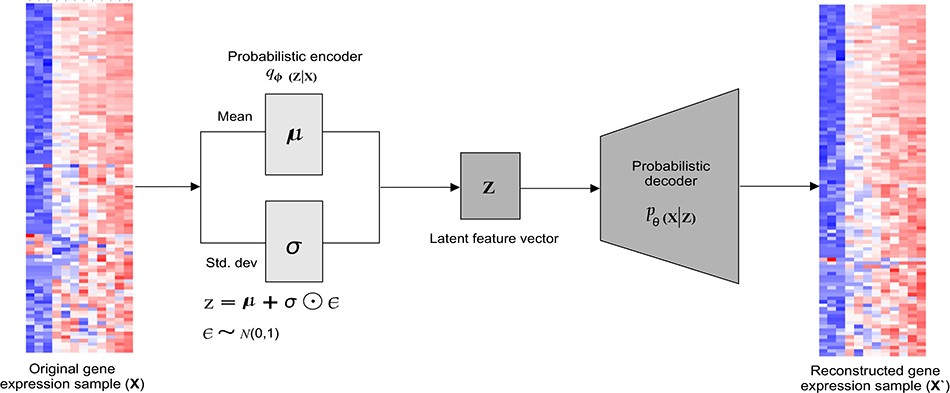
\includegraphics[width=\textwidth]{karim2021_vae.jpeg}
            \caption[\textit{Variational autoencoder}: arquitectura]{
                Representació esquemàtica d'una arquitectura \gls{vae}.
                El codificador aprèn a representar l'entrada $\mathbf{x}$
                en un espai latent $\mathbf{z}$
                que segueix una distribució normal multivariant,
                amb un vector de mitjanes $\mu$ i un vector de variancies $\sigma$.
                S'utilitza la reparametrització de $\mathbf{z}$ en funció de $\epsilon$.
                El descodificador reconstrueix l'entrada
                a partir de la representació a l'espai latent.
                Font: Karim \textit{et. al.}, 2021 \citep{Karim2021}
            }
            \label{f:vae_min}
        \end{figure}

    \subsection{Variational Deep Embedding}
    \label{s:metodes_vade}

        El model \gls{vade} generalitza el model \gls{vae}
        utilitzant un model \gls{gmm}
        en lloc d'una normal multivariant,
        com s'il·lustra a la \cref{f:vade}.
        Això fa que siguin un model molt més
        apropiat per realitzar \textit{clustering},
        i manté la propietat generadora del \gls{vae}.

        Així, la principal diferència és que la \gls{cr}
        està formada per $\pi$ distribucions normals multivariants.
        El codificador aproxima una distribució conjunta
        de $\mathbf{x}$, $\mathbf{z}$ i $c$ (el clúster):
        \begin{equation}
            \label{eq:vade_joint}
            p(\mathbf{x}, \mathbf{z}, c) =
            p(\mathbf{x}|\mathbf{z}) p(\mathbf{z}|c) p(c)
        \end{equation}

        on les probabilitats són:
        \begin{gather}
            \label{eq:vade_prob}
            p(c) = Cat(c|\pi)
            \\
            p(\mathbf{z}|c) = \mathcal{N} (\mu_c, \sigma^2_c \mathbf{I})
            \\
            p(\mathbf{x}|\mathbf{z}) = \mathcal{N} (\mathbf{x}|\mu_x, \sigma^2_x \mathbf{I})
        \end{gather}

        on $Cat(c|\pi)$ és la distribució dels clústers
        i $\mu_c$ i $\sigma^2_c$ són la mitjana i variància
        corresponents al clúster $c$.

        El procés generatiu es realitza
        escollint un clúster $c$,
        i realitzant el mateix procés que en el model \gls{vae}
        per obtenir la reconstrucció,
        utilitzant la corresponent distribució normal.

        Durant la fase d'entrenament,
        el model s'optimitza utilitzant les mateixes funcions de cost
        de reconstrucció i regularització,
        utilitzant el mètode de la reparametrització de $\mathbf{z}$
        i una fórmula més complexa per calcular el \gls{elbo}.
        Donat que el procés és similar al \gls{vae},
        no s'ha considerat necessari desenvolupar les fórmules matemàtiques.

        \begin{figure}
            \centering
            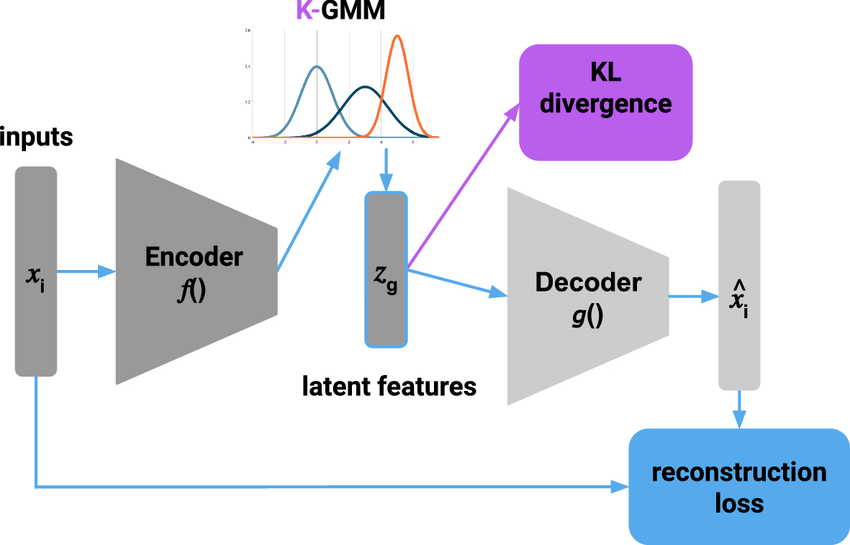
\includegraphics[width=0.7\textwidth]{lafabregue2022_vade.png}
            \caption[Esquema model VaDE]{
                Representació esquemàtica de l'arquitectura del model \gls{vade}.
                Font: Lafabregue \textit{et. al.}, 2022 \citep{Lafabregue2022}
            }
            \label{f:vade}
        \end{figure}


    \section{Mètriques d'avaluació}
    \label{s:metrics}

        Per validar la \gls{qc}
        s'han utilitzat dos tipus de mètriques:
        validació externa i validació interna.
        Les mètriques de validació externa
        es basen en comparar els clústers obtinguts
        amb una partició de les dades coneguda prèviament,
        que es considera la partició \textit{correcta}.
        Les mètriques de validació interna
        no utilitzen dades externes i
        es basen en mesures observables
        en la pròpia estructura dels clústers.

        Donat que la tècnica de \textit{clustering}
        és una tècnica d'aprenentatge no supervisada,
        normalment s'utilitzen exclusivament les mètriques de validació interna
        ja que no es coneix l'estructura real de les dades.
        En el cas d'aquest \gls{tfm},
        les dades utilitzades provenen d'un estudi clínic
        i estan etiquetades segons el diagnòstic de cada pacient,
        per tant s'han pogut utilitzar també mètriques de validació externa.

        Cap mètrica per si sola és eficaç
        per avaluar la \gls{qc} \cite{Palacio-Nino2019},
        de manera que s'han seleccionat quatre mètriques:
        una basada en validació interna
        i tres basades en validació externa.
        Es descriuen a continuació:

        \paragraph{Mètriques de validació interna}
            La \gls{qc} es pot mesurar en funció de
            la cohesió
            (la proximitat entre els elements dins d'un mateix clúster),
            i el nivell de separació entre els diferents clústers.

%            \newacronym{sse}{SSE}{suma de quadrats dels errors dintre de clústers
%                                  (\textit{sum of squared errors within clusters})}
%            \newacronym{ssb}{SSB}{suma de quadrats dels errors entre clústers
%                                  (\textit{sum of squared errors between clusters})}
%            \newacronym{ch}{CH}{coefficient de Calisnki-Harabasz}
%
%            La cohesió es pot mesurar
%            mitjançant la \gls{sse}:
%            \begin{equation}
%            \label{eq:sse}
%                SSE(C_i) = \sum_{x \in C_i} d(c_i, x)^2
%            \end{equation}
%            on $x$ és un punt dintre del clúster $C_i$
%            i $c_i$ és el centroide del clúster.
%
%            De manera similar,
%            el nivell de separació es pot mesurar
%            mitjançant la \gls{ssb}:
%            \begin{equation}
%            \label{eq:ssn}
%                SSB = \sum_{i=1}^{K} m_i d(c_i, c)^2
%            \end{equation}
%            on $m_i$ és el nombre d'observacions
%            en el clúster $i$,
%            $c_i$ el seu centroide
%            i $c$ la mitjana global.
%
%            Les dues mesures es poden combinar en una sola mètrica
%            utilitzant el \gls{ch}:
%            \begin{equation}
%            \label{eq:ch}
%                CH = \frac
%                { \frac{SSB_M}{M-1} }
%                { \frac{SSE_M}{M} }
%            \end{equation}
%            on $M$ és el nombre de clústers.


            Una de les mètriques més comuns
            per avaluar aquestes dues característiques
            és el coeficient silueta.
            Es computa de la següent manera,
            segons les equacions a continuació:
            per cada punt $i$ es computen
            la distància mitja $a(i)$ a tots els punts $j$ dins el mateix cluster $C_a$,
            la mínima distància mitja $b(i)$ a tots els punts $j$ dins cada cluster $C_b$ diferent de $C_a$
            i el seu coeficient silueta $s(i)$.
            Finalment, es computa la silueta global $S$
            prenent la mitjana de les siluetes de tots els punts.

            \begin{gather}
                a(i) = \frac{1}{|C_a|}
                \sum_{j \in C_a, i \neq j} d(i,j)
                \\
                b(i) = \min_{C_b \neq C_a}
                \frac{1}{|C_b|}
                \sum_{j \in C_b} d(i,j)
                \\
                s(i) = \frac
                {b(i) - a(i)}
                {\max \{a(i), b(i)\}}
                \\
                \label{eq:sil}
                Sil. = \frac{1}{n}
                \sum_{i=1}^{n} s(i)
            \end{gather}

            El coeficients silueta pren un valor en l'interval $[-1, 1]$,
            on valors positius indiquen una bona separació entre clústers,
            valors negatius indiquen que els clústers estan barrejats entre ells,
            i un coeficient de zero indica que les dades estan distribuïdes uniformement.

        \paragraph{Mètriques de validació externa}
            Si es té una partició de referència $P$,
            la \gls{qc} es pot mesurar comparant-la
            amb els clústers $C$ resultants de l'algoritme de \textit{clustering}.
            Es construeix un taula de contingència
            i es comparen les parelles d'observacions
            trobades en el mateix o diferents clústers
            en les particions $P$ i $C$.
            S'extreuen els següents indicadors:
            \begin{description}
                \item[TP]
                nombre de parelles trobades al mateix clúster
                tant en $C$ com en $P$.

                \item[FP] nombre de parelles trobades al mateix clúster en $C$,
                però en diferents clústers en $P$.

                \item[TN] nombre de parelles trobades en diferents clústers
                tant en $C$ com en $P$.

                \item[FP] nombre de parelles trobades en diferents clústers en $C$,
                però en el mateix clúster en $P$.
            \end{description}

            Amb aquests indicadors
            es pot computar una gran varietat de mètriques,
            que es poden classificar diverses famílies \citep{Palacio-Nino2019}.
            \begin{itemize}
                \item La família de conjunts coincidents
                es basa en assignar una correspondència
                entre els clusters $C$ i les particions $P$,
                i mesurar la similaritat entre els conjunts.

                \item La família d'igual a igual parteix de l'assumpció
                que les observacions que es troben a la mateixa partició a $P$
                haurien d'esta també al mateix clúster $C$,
                i es basen en les correlacions entre parelles d'observacions.

                \item La tercera família es basa
                en conceptes de la teoria de la informació.
            \end{itemize}

            S'ha seleccionat una mètrica de cada família, respectivament:
            l'exactitud, l'\gls{ari} i el coeficient d'\gls{ami}.

            \subparagraph{Exactitud}
                L'exactitud (\textit{accuracy})
                mesura la proporció d'elements classificats correctament,
                és a dir la proporció de coincidències
                entre assignacions dels clústers i les classes reals:
                \begin{equation}
                \label{eq:accuracy}
                    Acc. = \frac{TP + TN}{TP + TN + FP + FN}
                \end{equation}

                Pel seu càlcul,
                és necessari primer associar cada clúster
                a una de les classes reals.
                S'ha associat a cada clúster
                la classe que obté la major freqüència.

            \subparagraph{\gls{ari}}
                Calcula la similaritat entre les particions $C$ i $P$
                com la proporció d'el nombre d'elements classificats correctament
                respecte el nombre total d'elements,
                corregit per la probabilitat de cada clúster.
                \begin{equation}
                \label{eq:rand}
                    ARI = \frac{
                              \sum_{ij} \binom{n_{ij}}{2}
                              - [\sum_{i} \binom{c_i}{2} \sum_{j} \binom{p_j}{2}]
                              / \binom{n}{2}
                          }{ \frac{1}{2}
                              [\sum_{i} \binom{c_i}{2} + \sum_{j} \binom{p_j}{2}]
                              - [\sum_{i} \binom{c_i}{2} \sum_{j} \binom{p_j}{2}]
                              / \binom{n}{2}
                          }
                \end{equation}

                on $n_ij$ són els elements d'una matriu de contingència
                de les particions $C$ i $P$,
                $p_i$ i $c_i$ són el número d'elements de les particions de $P$ i $C$.

            \subparagraph{\gls{ami}}
                Mesura la reducció en la incertesa
                de l'assignació dels clústers $C$
                donada la partició coneguda $P$,
                corregit per la probabilitat de cada clúster.
                \begin{gather}
                \label{eq:mi}
                    MI(P,C) = \sum_i \sum_j p_{ij} \log \frac{p_{ij}}{p_i p_j}
                    \\
                    H(P) = - \sum_{j=1}^p P_P(j) \log P_P(j)
                    \\
                    H(C) = - \sum_{j=1}^c P_C(j) \log P_C(j)
                    \\
                    AMI = \frac{MI(P,C) - \mathbb{E}(MI(P,C))}
                    {\max\{H(P), H(C)\} - \mathbb{E}(MI(P,C))}
                \end{gather}

                on $p$ i $c$ són el número de particions de $P$ i $C$.


    \section{Conjunts de dades}
    \label{s:dades}

    Per comparar els resultats dels diferents mètodes de \textit{clustering}
    s'han utilitzat tres conjunts de dades,
    dos d'accés públic i un privat.

    \paragraph{\acrshort{mnist}}
        El conjunt de dades \gls{mnist} \citep{Deng2012}
        és un conjunt de dades freqüentment utilitzat
        per l'entrenament de models de \textit{machine learning},
        especialment amb els relacionats amb el reconeixement o processat d'imatges.

        Es tracta d'un conjunt de 70.000 imatges
        de dígits escrits a mà,
        etiquetades en funció del dígit que representen.
        Cada imatge té una resolució de 28 x 28 píxels.
        En aquest \gls{tfm}, s'ha tractat cada imatge com una observació
        i els 784 píxels com 784 variables independents.

    \paragraph{Exposome Data Challenge Event}
        Es tracta de diversos conjunts de dades
        provinents d'un concurs anomenat \textit{Exposome Data Challenge Event} \citep{Maitre2022},
        que va tenir lloc a l'abril de 2021.
        En aquest concurs es van presentar una sèrie de conjunts de dades
        metabolòmiques, proteòmiques, de metilació del ADN i d'exposició ambiental
        observades en nens entre 6 i 11 anys,
        a més de dades fenotípiques
        i de covariables o possibles factors de confusió.

        L'objectiu del concurs era que els competidors
        presentessin formes innovadores d'analitzar les dades
        i trobar relacions rellevants en l'àmbit de la salut.

        S'han seleccionat dos conjunts de dades
        sobre els que comparar les diferents tècniques de \textit{clustering}:

        \begin{itemize}
            \item Dades metabolòmiques, formades per dos conjunts de dades,
            extretes de mostres de sèrum (177 metabolits) i orina (44 metabolits),
            formant un total de 221 variables.

            \item Dades d'exposició ambiental o exposoma,
            compostes per 222 indicadors d'exposició
            relacionats amb l'exposició a factors ambientals
            (contaminació de l'aire, soroll),
            l'exposició a productes químics
            (metalls, pesticides)
            i l'estil de vida dels individus
            (dieta, consum de tabac).
        \end{itemize}

        Per mesurar les mètriques de validació externa,
        s'han seleccionat algunes variables fenotípiques i de les covariables
        que s'han trobat que poden ser descriptives.

        En tots els casos,
        s'ha seleccionat només aquelles observacions
        que contenen dades a tots els conjunts de dades.
        En total, es disposa de 1152 observacions.

    \paragraph{Dades \acrshort{privades}}
        En tercer lloc,
        s'ha utilitzat un conjunt de dades metabolòmiques
        facilitat pel grup de recerca
        \textit{Biomarkers and Nutritional \& Food Metabolomics}\footnote{\url{http://www.nutrimetabolomics.com/}},
        del Departament de Nutrició, Ciències de l'Alimentació i Gastronomia
        de la Universitat de Barcelona\footnote{\url{https://www.ub.edu/web/ub/ca/universitat/campus_fac_dep/departaments/n/depnutricioCAiG.html?}}.

        Les dades provenen d'un estudi clínic titulat
        \gls{privades} \citep{Petersen2022},
        que pretén desenvolupar tècniques innovadores
        per estudiar la relació entre els gens, la dieta i l'estil de vida
        amb càncer i altres malalties,
        aplicant una perspectiva trans-generacional.

        Es tracta d'un conjunt de 1120 observacions
        sobre 411 metabòlits
        obtingudes en tres moments diferents sobre els mateixos pacients,
        acompanyades de 16 covariables
        de les quals dues són categòriques
        (gènere, índex de risc de malalties cardiovasculars)
        i la resta numèriques
        (edat i diversos indicadors de salut).

        L'equip de recerca que ha proveït les dades
        ha anonimitzat la identitat dels pacients
        i ha prohibit expressament la publicació de les dades
        per protegir la seva confidencialitat.



    \section{Metodologia}
    \label{s:metodologia}

    A continuació es descriu la metodologia que s'ha seguit
    per avaluar els diferents mètodes de \textit{clustering}
    utilitzant els tres conjunts de dades estudiats.

    Tot el codi utilitzat per implementar els models de \textit{deep clustering}
    i per dur a terme la metodologia que s'explica a continuació
    s'ha fet públic a un repositori de GitHub:
    \url{https://github.com/carlescn/MSc_bioinformatics_thesis}.

    Per cada conjunt de dades,
    s'han seguit els següents passos
    amb algunes variacions que s'expliquen a continuació.
    A la \cref{t:metodes_resum} es resumeixen totes les tècniques
    avaluades per cada conjunt de dades.

    \paragraph{Seleccionar classes de referència}
        Primerament s'ha seleccionat una o diverses variables categòriques independents,
        que permetin separar les observacions en grups de referència
        contra els que comparar els clústers obtinguts
        i calcular les mètriques de validació externa.

        El nombre de classes de cada una d'aquestes variables
        ha determinat el nombre de clústers que s'ha fixat per cada una de les tècniques.
        En els casos en que s'han escollit variables amb diferents nombres de classes,
        s'han repetit tots els mètodes pels respectius números de clústers.

        En el cas que les variables escollides siguin numèriques i contínues,
        s'han codificat artificialment en quatre grups utilitzant quantils.

    \paragraph{Normalitzar les dades}
        Els conjunts de dades s'han normalitzat
        aplicant la funció \textit{min-max}
        per acotar tots els valors dins d'un rang entre 0 i 1.
        D'aquesta manera s'aconsegueix
        adaptar les dades a un format que els models de \textit{deep learning} puguin tractar,
        i reduir els possibles efectes d'escala de les diferents variables.

    \paragraph{Tècniques clàssiques}
        A continuació
        s'han aplicat les tècniques de \textit{clustering} clàssiques seleccionades
        (\gls{kmeans}, \gls{gmm}, \gls{aglo})
        sobre les dades sense tractar.

        Després s'ha aplicat \gls{pca}
        i s'han seleccionat les primeres components principals
        que expliquen el 80\% de la variància.
        S'han repetit les tècniques clàssiques
        sobre les dades transformades.

        Les mètriques obtingudes amb aquest mètodes
        s'han pres com a mesura de referència
        contra la que comparar el rendiment de les tècniques de \textit{deep clustering}.

    \paragraph{Mètodes de \textit{deep learning}}
        Seguidament
        s'han avaluat diversos mètodes de \textit{deep clustering}.
        Tots els models implementats es basen en un \gls{ae}
        amb codificador i descodificador simètrics
        basats en \gls{mlp}.
        El primer pas ha sigut buscar una configuració òptima del \gls{ae}.

        Donat que (tret de les dades \gls{mnist}) els conjunts de dades són relativament petits,
        s'ha intentat reduir al màxim el nombre de paràmetres entrenables de la xarxa neuronal.
        S'han provat diverses configuracions de nombre i mida de les capes internes
        i s'ha seleccionat la que aconsegueix reduir el nombre de paràmetres
        sense afectar negativament a la puntuació de la funció de cost.

        El nombre de neurones de la capa latent
        (així com de la capa de \textit{clustering} quan aplica)
        s'ha fixat al nombre de clústers que es vol obtenir.

        En tots els casos,
        per totes les neurones s'ha establert la funció d'activació \gls{relu},
        excepte les capes d'entrada del codificador i descodificador,
        així com la sortida del codificador (capa latent),
        que no tenen funció d'activació,
        i la sortida del descodificador (sortida de reconstrucció de l'autoencoder),
        que té funció d'activació sigmoide.

        Un cop seleccionada la configuració,
        s'ha entrenat i avaluat els models \gls{dec} i \gls{vade}
        per cada un dels conjunts de dades
        i números de clústers escollits.

    \paragraph{Avaluació dels resultats}
        Finalment,
        s'han compilat totes les mètriques
        i s'han comparat els clústers obtinguts
        mitjançant representacions gràfiques.

        Per cada tècnica i número de clústers
        s'han visualitzat el conjunt de dades
        (originals o transformades, segons la tècnica utilitzada)
        en un núvol de punts de dues dimensions
        mitjançant la tècnica \gls{tsne},
        assignant un color diferent a cada clúster (\cref{f:ex_tsne}).

        \begin{figure}
        \begin{minipage}[c]{0.48\textwidth}
            \centering
            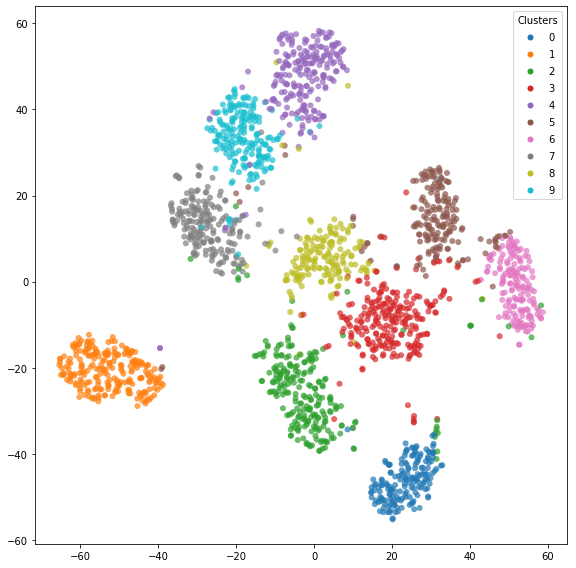
\includegraphics[width=6cm]{exemple_tsne_vademnist.png}
            \caption[Exemple gràfica t-SNE]{
                Exemple de gràfica \gls{tsne}
                del model \gls{vade} entrenat sobre les dades \gls{mnist}.
                Es representa la \gls{cr} utilitzant ls dues primers components
                de la reducció \gls{tsne}.
                Els colors mostren els les assignacions de clústers del model.
            }
            \label{f:ex_tsne}
        \end{minipage} \hfill
        \begin{minipage}[c]{0.48\textwidth}
            \centering
            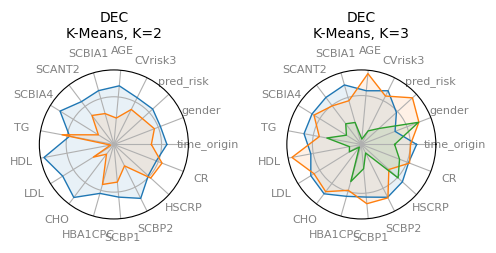
\includegraphics[width=7cm]{exemple_radialplots_dchng.png}
            \caption[Exemple gràfica radial]{
                Exemple de gràfica radial.
                Es representa la distribució multivariant de les covariables
                del conjunt de dades \gls{privades}
                en funció de les assignacions de clústers
                trobades pel model \gls{dec},
                fixant el número de clústers a 2 i 3.
                Cada radi del diagrama representa una variable,
                i els polígons del centre representen la distribució multivariant que pren cada clúster,
                on cada vèrtex és la mitjana dels valors per cada variable.
            }
            \label{f:ex_radial}
        \end{minipage}
        \end{figure}

        Mitjançant gràfiques radials  (\cref{f:ex_radial}),
        s'ha representat la distribució multivariant
        de les variables independents
        pels clústers trobats amb cada combinació de tècnica i nombre de clústers.

        S'han seleccionat les 20 variables amb més variabilitat de cada conjunt de dades
        i s'ha representat la seva distribució multivariant
        pels diferents clústers de la mateixa manera.



        Per últim,
        s'han comparat entre elles les assignacions de clústers de cada un dels mètodes
        mitjançant un gràfic tipus \textit{heatmap}  (\cref{f:ex_heatmap}),
        on cada fila representa una de les tècniques avaluades,
        les columnes representen les observacions del conjunt de dades,
        i el color representa l'assignació de cada mostra a un dels clústers.

        \begin{figure}
            \centering
            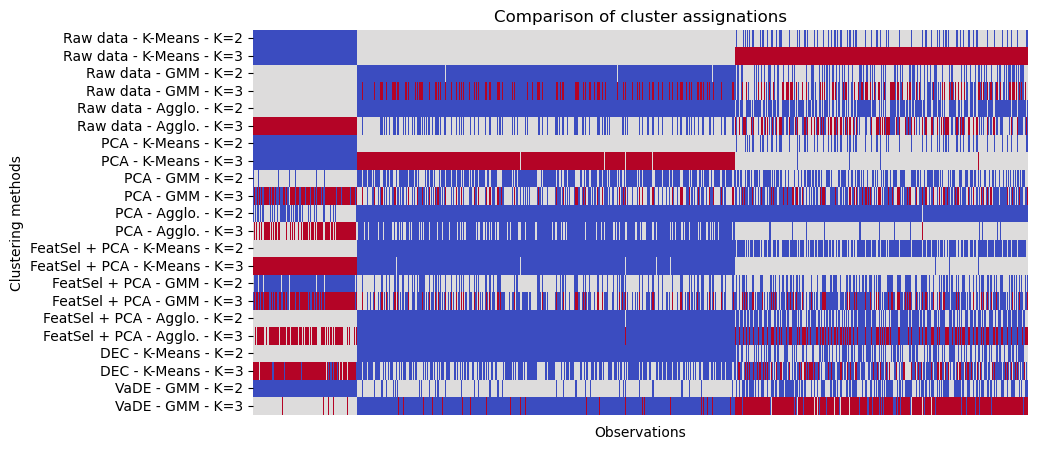
\includegraphics[width=\textwidth]{exemple_heatmap_dchng.png}
            \caption[Exemple gràfica \textit{heatmap} de les assignacions de clústers]{
                Exemple de gràfica \textit{heatmap}
                on es comparen els clústers trobats pels diferents mètodes
                avaluats sobre el conjunt de dades \gls{privades}.
                Cada fila representa una de les tècniques,
                les columnes representen les observacions
                i el colors representen a quin clúster s'ha assignat cada observació.
                Per poder comparar les tècniques,
                totes les files s'han ordenat segons el mateix índex.
            }
            \label{f:ex_heatmap}
        \end{figure}


        \subsection{MNIST}
        \label{s:mnist}

            El conjunt de dades \gls{mnist}
            s'ha seleccionat per ser un exemple molt estudiat
            i sobre el que es coneix que
            es poden aconseguir bons resultats de \textit{clustering}
            amb diferents mètodes, clàssics i basats en \textit{deep learning}.

            S'ha utilitzat com a marc de referència
            per validar la funcionalitat
            dels diferents models de \textit{deep clustering} implementats,
            i seleccionar aquells que funcionin millor.

            El nombre de clústers s'ha fixat en 10,
            ja que només s'han comparat amb les etiquetes de les imatges.

            \paragraph{Mètodes clàssics}
                Només s'han avaluat les tècniques \gls{kmeans} i \gls{gmm}.

            \paragraph{Mètodes de \textit{deep clustering}}
                En tots els casos s'ha utilitzat
                el mateix subcojunt de 60.000 imatges per entrenar el model
                i les 10.000 restants per avaluar el seu rendiment.

                S'ha escollit una configuració del \gls{ae},
                que es coneix dona bons resultats en aquest conjunt de dades \citep{Xie2015}:
                tres capes ocultes amb mides 512, 512 i 2048.

                S'han contrastat els següents mètodes:

                \begin{itemize}
                    \item Entrenar un model \gls{ae} amb les dades d'entrenament,
                    codificar les dades de validació
                    i aplicar \gls{kmeans} i \gls{gmm}
                    sobre les dades transformades (capa latent).

                    \item Repetir la mateixa operació amb un model \gls{vae}.

                    \item Entrenar i avaluar un model \gls{dec},
                    inicialitzant els paràmetres del model
                    primer amb \gls{kmeans} i amb \gls{gmm}.

                    \item Entrenar i avaluar un model mixt \gls{vae}+\gls{dec},
                    que reemplaça el \gls{ae} de l'arquitectura \gls{dec}
                    per un \gls{vae}.
                    Els paràmetres s'han inicialitzat amb \gls{kmeans} i amb \gls{gmm}.

                    \item Repetir la mateixa operació,
                    però mantenint el descodificador del model \gls{vae}
                    i afegint la funció de cost de reconstrucció
                    durant l'entrenament.

                    \item Entrenar i avaluar un model \gls{vade},
                    inicialitzant els paràmetres amb \gls{gmm}.
                \end{itemize}


            \paragraph{Avaluació dels mètodes}
                Finalment,
                s'han comparat totes les mètriques
                i s'han seleccionat aquells models de \textit{deep learning}
                que mostren un bon rendiment en relació amb la seva complexitat:
                \gls{dec} i \gls{vade}.

                S'han comparat els clústers trobats per les diferents tècniques
                utilitzant les representacions \gls{tsne} de les dades.
                No s'han representat els gràfics radials multivariants.


        \subsection{Exposome Data Challenge Event}
        \label{s:exposome}

            Amb aquest conjunt de dades s'han comparat
            tres tècniques de \textit{clustering} clàssiques
            amb els dos models de \textit{deep clustering}
            seleccionats al pas anterior
            (\gls{dec}, \gls{vade}).
            Donat que en aquest cas sí es tracta de dades metabolòmiques,
            s'espera que el resultat sigui extrapolable
            a altres conjunts de dades del mateix tipus.

            S'han seleccionat 11 variables independents
            (veure \cref{t:exposome_vars}).
            Per tant, s'han avaluat les tècniques
            pels fixant el nombre de clústers a 2, 3, 4, 6 i 7.

%            \setlength\arrayrulewidth{1pt}
            \begin{table}[h]
                \small
                \centering
                \begin{tabular}{@{}cccl@{}}
                    \toprule
                    \textbf{Grup de covars.}
                    & \textbf{Nom}
                    & \textbf{Núm. classes}
                    & \textbf{Descripció}  \\ \midrule
                    Fenotip     & birth\_weight & 4\textsuperscript{*} & Pes al néixer.                      \\
                    Fenotip     & iq            & 4\textsuperscript{*} & Quocient d'intel·ligència.          \\
                    Fenotip     & behaviour     & 4\textsuperscript{*} & Comportament neurològic (índex).    \\
                    Fenotip     & asthma        & 2                    & Incidència d'asma.                  \\
                    Fenotip     & bmi           & 4\textsuperscript{*} & Índex de massa corporal.            \\
                    Covariables & cohort        & 6                    & Cohort d'inclusió a l'estudi.       \\
                    Covariables & age           & 7                    & Edat en anys.                       \\
                    Covariables & sex           & 2                    & Gènere.                             \\
                    Covariables & education     & 3                    & Nivell d'estudis de la mare.        \\
                    Covariables & native        & 3                    & Pares natius del país de naixement. \\
                    Covariables & parity        & 3                    & Nombre d'embarassos previs (mare).  \\ \bottomrule
                \end{tabular}
                \caption[Exposome Data Challenge Event: covariables seleccionades]{
                    Variables independents seleccionades del conjunt de dades Exposome Data Challenge Event.
                    \newline \textsuperscript{*}Variables numèriques contínues,
                    convertides en 4 grups mitjançant quantils.}
                \label{t:exposome_vars}
            \end{table}

            S'han estudiat independentment dos conjunts de dades:
            les dades metabolòmiques
            (s'ha unit les lectures en sèrum i en orina
            per obtenir un conjunt de dades més gran)
            i les dades del exposoma.

            Per les tècniques de \textit{deep clustering},
            la configuració seleccionada del \gls{ae}
            és de tres capes internes amb mides 16, 16 i 128.

            \paragraph{Dades metabolòmiques}

                \subparagraph{Tècniques clàssiques}
                    S'han avaluat (\gls{kmeans}, \gls{gmm}, \gls{aglo})
                    sobre les dades originals i les transformacions \gls{pca}.

                    Addicionalment,
                    motivat pels resultats poc prometedors obtinguts,
                    s'han seleccionat les variables amb més variabilitat
                    (desviació estàndard superior a la mitjana del dataset,
                    avaluades per separat en les dades de sèrum i orina).
                    S'ha repetit l'avaluació dels mètodes sobre el conjunt de dades reduït.

                \subparagraph{Mètodes de \textit{deep clustering}}
                    S'ha entrenat i avaluat els dos models de \textit{deep clustering} seleccionats
                    (\gls{dec}, \gls{vade}).
                    Donat que els resultats inicials no han semblat molt prometedors,
                    s'ha intentat millorar la relació entre la mida de les dades
                    i el nombre de paràmetres de dues maneres:

                \begin{itemize}
                    \item Augmentar artificialment el nombre de dades.
                    S'han generat mostres aleatòries d'una distribució normal
                    amb mitjana 0 i desviació estàndard 0.01
                    (un ordre de magnitud inferior a la de les dades).

                    A continuació s'han sumat aquestes mostres als valors de les dades originals.
                    S'ha repetit el procés 10 vegades per obtenir un conjunt de dades
                    amb 11.520 observacions,
                    que presenten una distribució similar a les dades originals.

                    Amb aquestes dades,
                    s'han entrenat i avaluat els dos models de \textit{deep clustering.}

                    \item Reduir el nombre de paràmetres entrenables de la xarxa neuronal.
                    S'ha substituït les capes internes del tipus \gls{mlp} del \gls{ae}
                    per capes convolucionals, amb una i dues dimensions.
                    Això permet reduir dràsticament el nombre de paràmetres del model,
                    però assumeix que les dades presenten algun tipus d'estructura invariable.

                    S'ha necessitat adaptar les dades a una mida
                    d'entrada que aquests models puguin tractar.
                    Pel model amb capes convolucionals 1D,
                    s'han convertit els vectors de 221 valors de cada observació
                    en un vector 1D amb 224.
                    Pel model amb capes 2D,
                    s'han transformat en matrius bidimensionals de mida 16 x 16 (256 punts).
                    En ambdós casos s'han omplert amb zeros les posicions buides.

                    Per cada una de les dues configuracions (1D, 2D),
                    s'han seleccionat els paràmetres òptims del \gls{ae}.
                    Pel model 1D, una capa convolucional de mida 4. i mida del kernel 3.
                    Pel model 2D, dues capes convolucionals de mides 4 i 4, i mida del kernel 3.

                    Finalment,
                    s'han implementat i avaluat els quatre models de \textit{deep leraning}
                    (\gls{dec} i \gls{vade}, amb capes convolucionals 1D i 2D).
                \end{itemize}

            \paragraph{Dades de l'exposoma}

                \subparagraph{Tècniques clàssiques}
                    S'han avaluat (\gls{kmeans}, \gls{gmm}, \gls{aglo})
                    sobre les dades originals i les transformacions \gls{pca}.
                    No s'ha reduït la mida del conjunt de dades.

                \subparagraph{Mètodes de \textit{deep clustering}}
                    S'han avaluat els models \gls{dec} i \gls{vade}
                    basats en \gls{mlp}.
                    No s'han aplicat tècniques d'augment artificial de les dades
                    ni models amb capes convolucionals.

                \subparagraph{Correcció de l'efecte lot}
                    Els resultats obtinguts
                    suggereixen la presència d'un fort efecte de lot,
                    ja que totes les tècniques aconsegueixen un solapament gairebé perfecte
                    amb els grups de la variable \textit{cohort}.

                    Per aquest motiu,
                    s'ha decidit aplicar una correcció per aquest efecte lot als dos conjunts de dades.
                    Per cada classe de la variable \textit{cohort},
                    s'han estandarditzat els valors de cada variable
                    restant la mitjana i dividint per al desviació estàndard.
                    Les dades corregides obtingudes
                    s'han normalitzat de nou amb la funció \textit{min-max}.

                    Finalment,
                    s'han tornat a avaluar els mateixos cinc mètodes de clustering
                    (\gls{kmeans}, \gls{gmm}, \gls{aglo}, \gls{dec} i \gls{vade}).

            \paragraph{Avaluació dels models}
                S'han compilat les mètriques obtingudes amb totes les tècniques
                i s'han comparat les assignacions de clústers obtingudes
                mitjançant gràfiques \gls{tsne},
                gràfiques tipus heatmap
                i gràfiques radials per les distribucions multivariants
                de les covariables
                i de les 20 variables amb major variabilitat de cada conjunt de dades.

        \subsection{Dades DCH-NG}
        \label{s:dades_privades}

            Com a grups objectiu contra els que avaluar les mètriques
            s'han seleccionat dues variables categòriques de les covariables,
            que s'ha trobat mostren una distribució diferencial per la resta de covariables
            (indicadors biològics relacionats amb la salut) (veure \cref{t:dadespriv_vars}).
            Tots els mètodes s'han avaluat fixant el número de clústers a 2 i 3.

%            \setlength\arrayrulewidth{1pt}
            \begin{table}[h]
                \small
                \centering
                \begin{tabular}{@{}ccl@{}}
                    \toprule
                    \textbf{Nom} & \textbf{Núm. grups} & \textbf{Descripció}    \\ \midrule
                    gender       & 2 & Gènere de l'individu.                    \\
                    CVrisk3      & 3 & Risk de patir malalties cardiovasculars. \\
                    \bottomrule
                \end{tabular}
                \caption[Dades DCH-NG: covariables seleccionades]{Variables independents seleccionades del conjunt de dades \gls{privades}.}
                \label{t:dadespriv_vars}
            \end{table}

            \paragraph{Tècniques clàssiques}
                S'han avaluat (\gls{kmeans}, \gls{gmm}, \gls{aglo})
                sobre les dades originals i les transformacions \gls{pca}.

            \paragraph{Mètodes de \textit{deep clustering}}
                S'han avaluat els models \gls{dec} i \gls{vade}
                basats en \gls{mlp}.
                La configuració escollida per l'\gls{ae} de base
                és de dues capes amb 16 i 32 neurones.

            \paragraph{Avaluació dels models}
                Donat que les dades contenen mesures repetides sobre els mateixos individus,
                i s'espera que les variacions entre individus siguin majors
                que entre les observacions del mateix individu,
                s'ha calculat una mètrica addicional:
                la freqüència amb que les observacions del mateix individu
                s'assignen a un únic clúster (corregida per la mida del clúster).

                S'han compilat les mètriques obtingudes amb totes les tècniques
                i s'han comparat les assignacions de clústers obtingudes
                mitjançant gràfiques \gls{tsne},
                gràfiques tipus \textit{heatmap}
                i gràfiques radials per les distribucions multivariants
                de les covariables
                i de les 20 variables amb major variabilitat de cada conjunt de dades.

%        \setlength\arrayrulewidth{1pt}
        \begin{sidewaystable}[p]
            \small
            \centering
            \begin{tabular}{@{}cccccc@{}}
                \toprule
                \textbf{Conjunt de dades} & \textbf{Tipus} & \textbf{\textit{Feature learning}} & \textbf{\textit{Clustering}} & \textbf{Inicialització} & \textbf{Variacions} \\ \midrule
                \multirow{6}{*}{\textbf{MNIST}} & Clàssic & Cap, PCA & K-means, GMM & - & - \\
                & \multirow{5}{*}{\textit{Deep learning}} & AE & K-means, GMM & - & - \\
                &  & VAE & K-means, GMM & - & - \\
                &  & DEC & DEC & K-means, GMM & - \\
                &  & VAE+DEC & VAE+DEC & K-means, GMM & Mantenir descodificador \\
                &  & VaDE & VaDE & GMM & - \\ \midrule
                \multirow{6}{*}{\begin{tabular}[c]{@{}c@{}}\textbf{ExposomeChall.}\\ \textbf{(metaboloma)}\end{tabular}} & \multirow{2}{*}{Clàssic} & \multirow{2}{*}{Cap, PCA} & \multirow{2}{*}{K-means, GMM} & \multirow{2}{*}{-} & Selecció de variables, \\
                &  &  &  &  & Correcció efecte lot \\ \cmidrule(l){6-6}
                & \multirow{4}{*}{\textit{Deep learning}} & \multirow{2}{*}{DEC} & \multirow{2}{*}{DEC} & \multirow{2}{*}{K-means, GMM} & Selecció de variables, \\
                &  &  &  &  & Correcció efecte lot, \\
                &  & \multirow{2}{*}{VaDE} & \multirow{2}{*}{VaDE} & \multirow{2}{*}{GMM} & augment de dades, \\
                &  &  &  &  & conv 1D, 2D \\ \cmidrule(l){6-6}
                \multirow{3}{*}{\begin{tabular}[c]{@{}c@{}}\textbf{ExposomeChall.}\\ \textbf{(exposoma)}\end{tabular}} & Clàssic & Cap, PCA & K-means, GMM & - & \multirow{3}{*}{Correcció efecte lot} \\
                & \multirow{2}{*}{\textit{Deep learning}} & DEC & DEC & K-means, GMM &  \\
                &  & VaDE & VaDE & GMM &  \\ \midrule
                \multirow{3}{*}{\textbf{Dades DCH-NG}} & Clàssic & Cap, PCA & K-means, GMM & - & - \\
                & \multirow{2}{*}{\textit{Deep learning}} & DEC & DEC & K-means, GMM & - \\
                &  & VaDE & VaDE & GMM & - \\ \bottomrule
            \end{tabular}
            \caption[Tècniques de \textit{clustering} per conjunt de dades]{Resum de les tècniques de \textit{clustering}
                avaluades per cada conjunt de dades.}
            \label{t:metodes_resum}
        \end{sidewaystable}

    \section{Eines informàtiques}
    \label{s:software}

        \paragraph{Software}
            Els models de \textit{deep clustering}
            s'han implementat utilitzant el software Keras \citep{Chollet2015},
            una eina basada en TensorFlow \citep{Ghemawat2016}
            que es va desenvolupar per l'àmbit de la recerca.
            Permet definir i entrenar models de xarxes neuronals profunds
            de manera relativament senzilla,
            però alhora possibilita interactuar a més baix nivell amb TensorFlow
            per realitzar operacions més complexes \citep{Ketkar2021}.

            Pràcticament la totalitat de l'estudi
            s'ha realitzat mitjançant el llenguatge de programació Python \citep{VanRossum2009},
            documentat en llibretes Jupyter Notebook \citep{Kluyver2016}.
            Com s'ha mencionat al inici de la secció,
            tot el codi està disponible a un repositori a GitHub.

        \paragraph{Hardware i serveis de computació \textit{on-line}.}

            L'equip informàtic del que disposa l'estudiant,
            si bé té capacitat per executar les tècniques de \textit{clustering} clàssiques,
            presenta limitacions a l'hora d'entrenar models
            basats en xarxes neuronals profundes,
            que consumeixen una gran quantitat de memòria RAM
            i requereixen de GPUs potents per una execució més o menys àgil.

            Per aquest motiu,
            ha sigut imprescindible utilitzar un servei de computació \textit{on-line}.
            Concretament, s'ha utilitzat el servei de pagament Paperspace Gradient\footnote{\url{https://docs.paperspace.com/gradient/}}.
            A la \cref{c:economic} es desglossa el cost d'aquest servei.



\chapter{Resultats}
\label{c:resultats}
    %Detalleu en aquest apartat els resultats obtinguts utilitzant la metodologia descrita a l’apartat anterior.
    %Recull dels resultats del treball. Hauria d'haver-hi una correspondència amb la metodologia en el sentit que els resultats és el que s'obté després d'haver aplicat la metodologia.
    %Les figures han d'estar explicades i citades en el text, com la \ref{fig:my_label}, en la qual es mostra l'error en funció de la distància, en unitats arbitràries. A totes les gràfiques ha d'haver el títol dels eixos.
    %\begin{figure}[!htbp]
    %    \centering
    %    \includegraphics[width=7truecm]{Rplotmanh.png}
    %    \caption{Error en funcio de la distància en unitats arbitràries.}
    %    \label{fig:my_label}
    %\end{figure}

    \section{MNIST}
    \label{s:results_mnist}

        A la \cref{t:results_mnist} es mostren les mètriques
        obtingudes per cada un dels models avaluats.
        Les tècniques clàssiques aplicades sobre les dades sense transformar
        i sobre la transformació \gls{pca}
        han aconseguit el mateix rendiment,
        mentre que els models de \textit{deep clustering}
        en general han aconseguit un rendiment notablement més elevat.
        Això suggereix que les tècniques de \textit{deep learning}
        són capaces de trobar relacions no lineals
        que es perden al aplicar \gls{pca}.

        Dintre dels models de \textit{deep clustering},
        en referència a les mètriques de validació externa
        (és a dir, el grau de coincidència amb les etiquetes reals)
        cap destacat que els models basats en \gls{vae}
        són els que obtenen pitjor rendiment.

        Per altra banda, el model \gls{dec} pràcticament obté els mateixos resultats
        que aplicar tècniques clàssiques a la capa de representació del \gls{ae}.
        Això suggereix una alta dependència dels model \gls{dec}
        en els paràmetres amb què s'inicialitza durant l'entrenament.
        Ambdós obtenen els segons millors resultats.

        Els millors resultats per les mètriques de validació externa
        s'obtenen amb el model \gls{vade},
        que aconsegueix una exactitud de 94\%.

        Per últim, per la mètrica de validació interna
        el model \gls{dec} destaca sobre la resta.
        El model VAE+DEC on s'ha eliminat el descodificador
        obté una puntuació similar al \gls{dec},
        mentre que el model VAE+DEC que manté el descodificador
        perd aquesta capacitat.

        A la \cref{f:vaevadedec_comp} s'il·lustra
        la diferència entre els clústers obtinguts pels diferents models.
        El model \gls{vae}, encara que té certa capacitat per distingir els diferens grups,
        té dificultats per separar-los en la \gls{cr}
        donat que tots els punts comparteixen la mateixa distribució normal.
        En conseqüència, els clústers aconseguits aplicant \gls{gmm}
        mostren solapament.
        En comparació, els models \gls{vade} i \gls{dec}
        són capaços de separar els clústers i obtenir una millor \gls{qc}.

        \begin{table}[p]
            \small
            \centering
            \begin{minipage}{\textwidth}

            \begin{tabular}{@{}cccccccc@{}}
                \toprule
                \textbf{Tipus} & \textbf{\textit{Feature learning}} & \textbf{\textit{Clustering}} & \textbf{Inicialització} & \textbf{\gls{acc}} & \textbf{\gls{ari}} & \textbf{\gls{ami}} & \textbf{\gls{sil}} \\ \midrule
                \multirow{2}{*}{Clàssic} & \multirow{2}{*}{-} & K-means & - & 0.59 & 0.41 & 0.53 & 0.06 \\
                &  & GMM & - & 0.44 & 0.22 & 0.34 & 0.02 \\
                \multirow{13}{*}{\textit{Deep learning}} & \multirow{2}{*}{PCA} & K-Means & - & 0.59 & 0.41 & 0.53 & 0.09 \\
                &  & GMM & - & 0.47 & 0.23 & 0.43 & 0.02 \\  \midrule
                & \multirow{2}{*}{AE} & K-means & - & 0.83 & 0.69 & 0.73 & 0.19 \\
                &  & GMM & - & 0.77 & 0.57 & 0.68 & 0.14 \\
                & \multirow{2}{*}{DEC} & DEC & K-means & 0.83 & 0.69 & 0.74 & 0.93 \\
                &  & DEC & GMM & 0.76 & 0.56 & 0.69 & 0.93 \\
                & \multirow{2}{*}{VAE} & K-means & - & 0.59 & 0.41 & 0.54 & 0.16 \\
                &  & GMM & - & 0.48 & 0.25 & 0.39 & -0.01 \\
                & \multirow{2}{*}{VAE+DEC\textsuperscript{1}} & VAE+DEC\textsuperscript{1} & K-Means & 0.61 & 0.42 & 0.54 & 0.90 \\
                &  & VAE+DEC\textsuperscript{1} & GMM & 0.57 & 0.31 & 0.47 & 0.87 \\
                & \multirow{2}{*}{VAE+DEC\textsuperscript{2}} & VAE+DEC\textsuperscript{2} & K-means & 0.57 & 0.37 & 0.49 & 0.20 \\
                &  & VAE+DEC\textsuperscript{2} & GMM & 0.59 & 0.36 & 0.49 & 0.12 \\
                & VaDE & VaDE & GMM & 0.94 & 0.88 & 0.88 & 0.23 \\ \bottomrule
            \end{tabular}
            \caption[MNIST: resultats]{Resum dels resultats obtinguts sobre els conjunt de dades \gls{mnist}.
                \newline \textsuperscript{1} Model sense descodificador i per tant sense funció de cost de reconstrucció.
                \newline \textsuperscript{2} Model amb descodificador i funció de cost de reconstrucció.
            }
            \label{t:results_mnist}
            \end{minipage}
        \end{table}

        \begin{figure}[p]
            \centering
            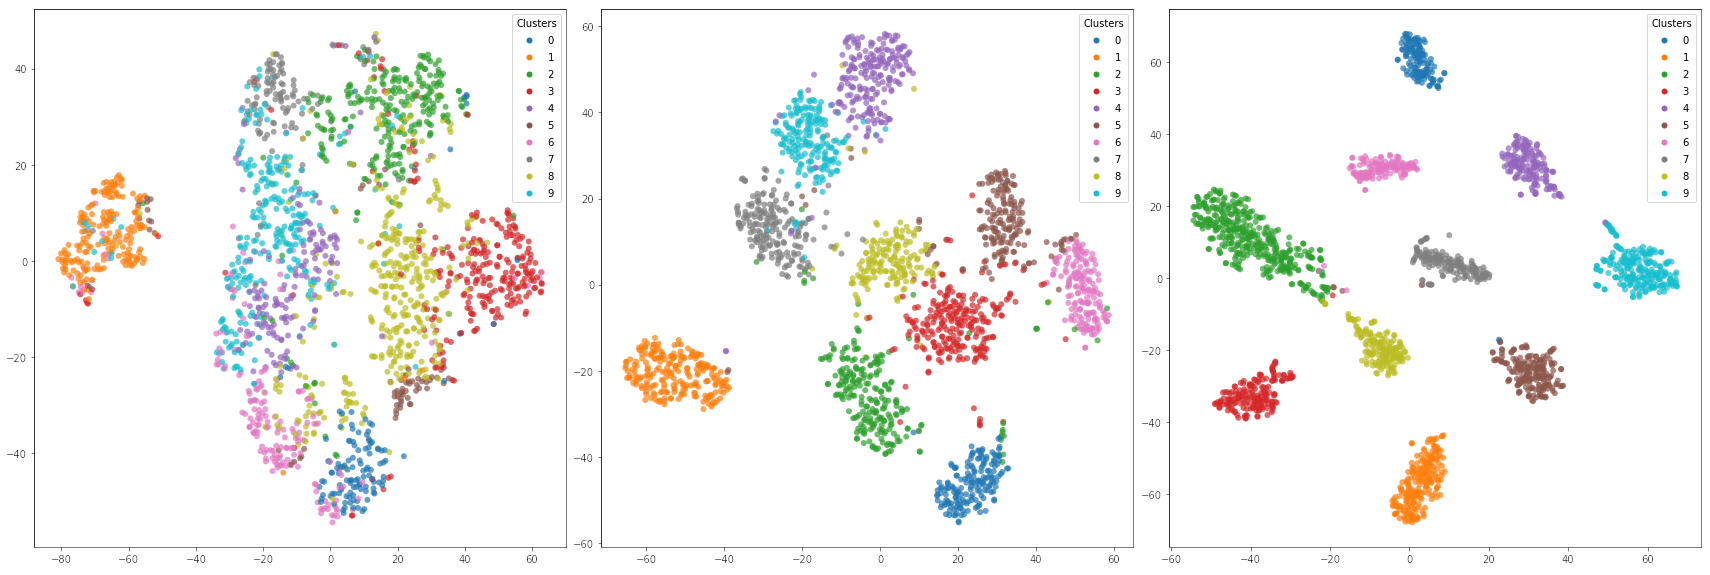
\includegraphics[width=\textwidth]{mnist/tsne_embeddings/vae_vade_dec_comparison.png}
            \caption[Comparació dels models VAE, VaDE i DEC]{
                Comparació dels models \gls{vae} + \gls{gmm} (esquerra), \gls{vade} (centre) i \gls{dec} (dreta).
                Representació \gls{tsne} de la \gls{cr} dels models.
                Els colors dels punts representen l'assignació a diferents clústers.
            }
            \label{f:vaevadedec_comp}
        \end{figure}


    \section{Exposome Data Challenge Event}
    \label{s:results_exposome}

        Les mètriques de validació mesurades en aquest conjunt de dades
        han resultat poc informatives.
        S'ha trobat que tots els models han aconseguit
        un solapament gairebé perfecte
        amb la covariable \textit{cohort},
        suggerint un fort efecte lot en les dades.

        No obstant,
        tot i aplicant una tècnica per corregir per aquest efecte,
        no s'ha trobat una relació clara entre els clústers
        i les covariables estudiades.

        Els mètodes addicionals que s'han estudiat
        (models convolucionals,
        selecció de variables amb més variació,
        augment artificial de les dades)
        no han aconseguit una millora en el rendiment.

        De nou, s'observa que el mètode \gls{dec}
        aconsegueix destacar-se reiteradament en quant a la mètrica silueta.

        A les \cref{t:metabol_results,t:exposome_results} es mostra
        per cada tècnica
        la mitjana de les mètriques obtingudes
        sobre els diferents números de clústers fixats.
        A la \cref{s:metodologia} s'explica amb més detall
        com interpretar aquesta gràfica.
        Els resultats complets s'adjunten al \cref{a:exposome}.

        Al comparar els clústers trobats per les diferents tècniques,
        s'observa un bon nivell de solapament entre totes les tècniques,
        amb l'excepció de \gls{gmm} aplicada sobre la transformació \gls{pca},
        que sembla trobar una estructura alternativa.

        A la \cref{f:expsome_heatmap} es mostra la comparació dels clústers
        trobats per les diferents tècniques avaluades
        sobre subconjunt de dades metabolòmiques corregides per l'efecte de lot.
        La resta de gràfiques s'adjunte al \cref{a:exposome}.

        Finalment,
        respecte a la distribució multivariant de les covariables,
        s'observa una possible distribució diferencial en funció dels lots
        que podria ser indicativa d'una interpretació biològica,
        però seria necessari un estudi multivariant posterior
        per treure'n conclusions.

        La distribució multivariant de les variables amb més variació
        no sembla mostrar una distribució diferencial en funció dels clústers,
        però com s'ha indicat abans caldria estudiar-ho amb més profunditat.

        A la \cref{f:expsome_radialplot} es mostra la distribució diferencial
        de les variables fenotípiques
        en funció dels clústers trobats pels diferents mètodes,
        fixant el número de clústers a 4.
        La resta de gràfiques s'adjunte al \cref{a:exposome}.

        \begin{figure}[p]
            \centering
            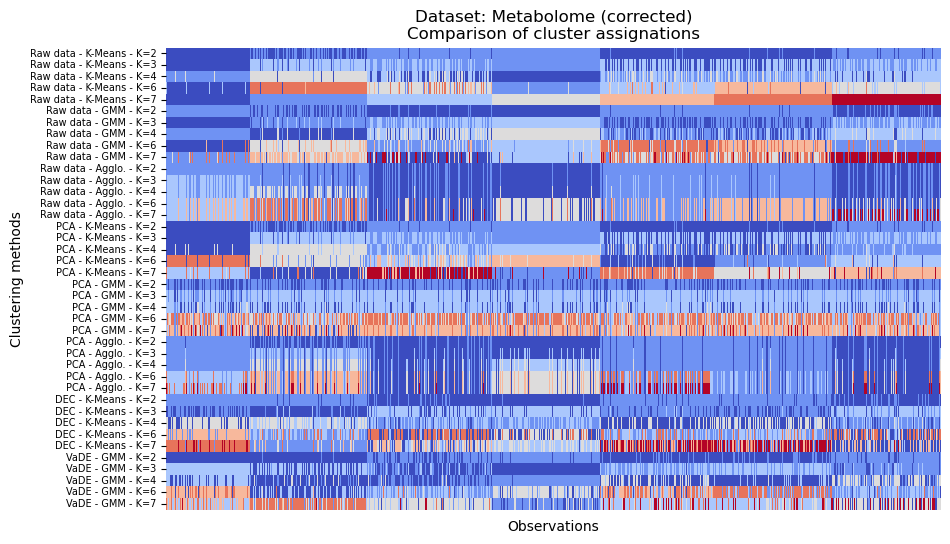
\includegraphics[width=\textwidth]{exposome_challenge/heatmap_clusters/metabol_corrected.png}
            \caption[Comparació dels clústers pel conjunt de dades Exposome Data Challenge Event]{
                Comparació dels clústers trobats pels diferents mètodes avaluats
                sobre el conjunt de dades Exposome Data Challenge Event,
                subconjunt dades metabolòmiques corregides per l'efecte de lot.
                S'observa un bon nivell de solapament entre totes les tècniques,
                excepte \gls{pca} + \gls{gmm} que sembla trobar una estructura alternativa.
            }
            \label{f:expsome_heatmap}
        \end{figure}

        \begin{figure}[p]
            \centering
            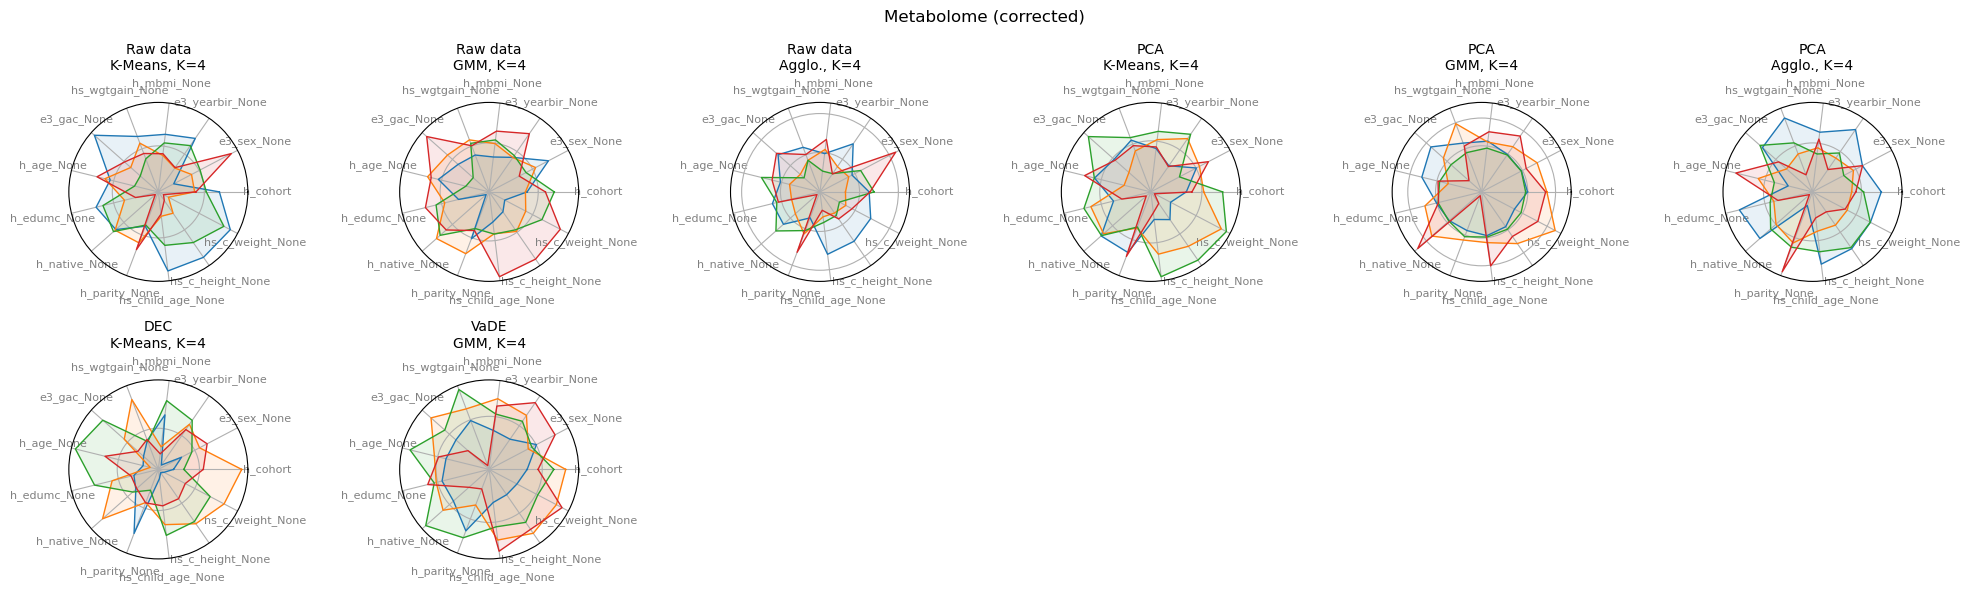
\includegraphics[width=\textwidth]{exposome_challenge/radialplots/metab_corr_covars_k4.png}
            \caption[Distribució diferencial de les variables fenotip a Exposome Data Challenge Event]{
                Representació de la distribució diferencial
                de les variables fenotípiques al conjunt de dades Exposome Data Challenge Event
                en funció dels clústers trobats pels diferents mètodes,
                fixant el número de clústers a 4.
            }
            \label{f:expsome_radialplot}
        \end{figure}

        \begin{table}[p]
            \small
            \centering
            \begin{tabular}{@{}ccccccccc@{}}
                \toprule
                \begin{tabular}[c]{@{}c@{}}Modificació\\ dades\end{tabular} & Tipus & \textit{Feature learning} & \textit{Clustering} & Inicialització & \gls{acc} & \gls{ari} & \gls{ami} & \gls{sil}\\ \midrule
                \multirow{13}{*}{-} & \multirow{6}{*}{Clàssic} & \multirow{3}{*}{PCA} & Agglo. & - & 0.46 & 0 & 0 & 0.06 \\
                &  &  & GMM & - & 0.46 & 0 & 0 & 0 \\
                &  &  & K-Means & - & 0.46 & 0 & 0 & 0.09 \\
                &  & \multirow{3}{*}{Raw data} & Agglo. & - & 0.46 & 0 & 0 & 0.05 \\
                &  &  & GMM & - & 0.46 & 0 & 0 & 0.06 \\
                &  &  & K-Means & - & 0.46 & 0 & 0 & 0.07 \\
                & \multirow{7}{*}{\textit{\begin{tabular}[c]{@{}c@{}}Deep\\ clustering\end{tabular}}} & DEC & DEC & K-Means & 0.48 & 0 & 0 & 0.54 \\
                &  & DEC + D.A. & DEC & K-Means & 0.48 & 0 & 0 & 0.83 \\
                &  & VaDE & VaDE & GMM & 0.48 & 0 & 0 & 0.17 \\
                &  & VaDE + D.A. & VaDE & GMM & 0.48 & 0 & 0 & 0.19 \\
                &  & DEC (conv. 1D) & DEC & K-Means & 0.48 & 0 & 0 & 0.69 \\
                &  & DEC (conv. 2D) & DEC & K-Means & 0.48 & 0 & 0 & 0.46 \\
                &  & VaDE (conv. 1D) & VaDE & GMM & 0.48 & 0 & 0 & 0.21 \\ \midrule
                \multirow{10}{*}{\begin{tabular}[c]{@{}c@{}}Selecció de\\ variables\end{tabular}} & \multirow{6}{*}{Clàssic} & \multirow{3}{*}{PCA} & Agglo. & - & 0.46 & 0 & 0 & 0.07 \\
                &  &  & GMM & - & 0.46 & 0 & 0 & 0.05 \\
                &  &  & K-Means & - & 0.46 & 0 & 0 & 0.08 \\
                &  & \multirow{3}{*}{Raw data} & Agglo. & - & 0.46 & 0 & 0 & 0.06 \\
                &  &  & GMM & - & 0.46 & 0 & 0 & 0.05 \\
                &  &  & K-Means & - & 0.46 & 0 & 0 & 0.07 \\
                & \multirow{4}{*}{\begin{tabular}[c]{@{}c@{}}Deep\\ clustering\end{tabular}} & DEC & DEC & K-Means & 0.48 & 0 & 0 & 0.5 \\
                &  & DEC (D.A.) & DEC & K-Means & 0.48 & 0 & 0 & 0.77 \\
                &  & VaDE & VaDE & GMM & 0.48 & 0 & 0 & 0.17 \\
                &  & VaDE (D.A.) & VaDE & GMM & 0.48 & 0 & 0 & 0.28 \\ \midrule
                \multirow{8}{*}{\begin{tabular}[c]{@{}c@{}}Correcció\\ efecte lot\end{tabular}} & \multirow{6}{*}{Clàssic} & \multirow{3}{*}{PCA} & Agglo. & - & 0.46 & 0 & 0 & 0.07 \\
                &  &  & GMM & - & 0.46 & 0 & 0 & 0.02 \\
                &  &  & K-Means & - & 0.46 & 0 & 0 & 0.09 \\
                &  & \multirow{3}{*}{Raw data} & Agglo. & - & 0.46 & 0 & 0 & 0.06 \\
                &  &  & GMM & - & 0.46 & 0 & 0 & 0.07 \\
                &  &  & K-Means & - & 0.46 & 0 & 0 & 0.07 \\
                & \multirow{2}{*}{\begin{tabular}[c]{@{}c@{}}Deep\\ clustering\end{tabular}} & DEC & DEC & K-Means & 0.48 & 0 & 0 & 0.49 \\
                &  & VaDE & VaDE & GMM & 0.48 & 0 & 0 & 0.22 \\\bottomrule
                \end{tabular}
            \caption[Exposome Data Challenge Event: resultats (metaboloma)]{
                Resum dels resultats obtinguts sobre el subcojunt de dades metabolòmiques
                del conjunt de dades Exposome Data Challenge Event
                (les puntuacions són la mitjana per tots els números de clústers avaluats).
                \textit{(D.A.): augment de dades}.
            }
            \label{t:metabol_results}
        \end{table}

        \begin{table}[p]
                \small
                \centering
                \begin{tabular}{@{}ccccccccc@{}}
                \toprule
                \begin{tabular}[c]{@{}c@{}}Modificació\\ dades\end{tabular}  & Tipus & \textit{Feature learning} & \textit{Clustering} & Inicialització & \gls{acc} & \gls{ari} & \gls{ami} & \gls{sil}\\ \midrule
                \multirow{8}{*}{-} & \multirow{6}{*}{Clàssic} & \multirow{3}{*}{PCA} & Agglo. & - & 0.6 & 0.17 & 0.18 & 0.13 \\
                &  &  & GMM & - & 0.59 & 0.16 & 0.18 & 0.11 \\
                &  &  & K-Means & - & 0.59 & 0.16 & 0.18 & 0.13 \\
                &  & \multirow{3}{*}{Raw data} & Agglo. & - & 0.6 & 0.17 & 0.18 & 0.1 \\
                &  &  & GMM & - & 0.59 & 0.17 & 0.19 & 0.1 \\
                &  &  & K-Means & - & 0.59 & 0.16 & 0.18 & 0.1 \\
                & \multirow{2}{*}{\begin{tabular}[c]{@{}c@{}}Deep\\ clustering\end{tabular}} & DEC & DEC & K-Means & 0.6 & 0.16 & 0.17 & 0.79 \\
                &  & VaDE & VaDE & GMM & 0.58 & 0.12 & 0.14 & 0.45 \\ \midrule
                \multirow{8}{*}{\begin{tabular}[c]{@{}c@{}}Correcció\\ efecte lot\end{tabular}} & \multirow{6}{*}{Clàssic} & \multirow{3}{*}{PCA} & Agglo. & - & 0.46 & 0 & 0 & 0.02 \\
                &  &  & GMM & - & 0.46 & 0 & 0 & 0.02 \\
                &  &  & K-Means & - & 0.47 & 0 & 0 & 0.03 \\
                &  & \multirow{3}{*}{Raw data} & Agglo. & - & 0.46 & 0 & 0 & 0.02 \\
                &  &  & GMM & - & 0.49 & 0.02 & 0.02 & 0 \\
                &  &  & K-Means & - & 0.47 & 0 & 0 & 0.02 \\
                & \multirow{2}{*}{\begin{tabular}[c]{@{}c@{}}Deep\\ clustering\end{tabular}} & DEC & DEC & K-Means & 0.48 & 0 & 0 & 0.64 \\
                &  & VaDE & VaDE & GMM & 0.48 & 0 & 0 & 0.27 \\ \bottomrule
            \end{tabular}
            \caption[Exposome Data Challenge Event: resultats (exposoma)]{
                Resum dels resultats obtinguts sobre el subcojunt de dades de l'exposoma
                del conjunt de dades Exposome Data Challenge Event
                (les puntuacions són la mitjana per tots els números de clústers avaluats).}
            \label{t:exposome_results}
        \end{table}

    \section{Dades DCH-NG}
    \label{s:results_privades}

        De nou, les mètriques de validació mesurades en aquest conjunt de dades
        han resultat poc informatives:
        cap dels mètodes ha aconseguit un bon rendiment
        respecte a les mètriques de validació externes.
        Respecte a la mètrica silueta,
        de nou el model \gls{dec} destaca significativament.

        Encara que els clústers obtinguts no mostren correlació
        amb les covariables categòriques preses com a referència,
        sí mostren un alt nivell de solapament
        entre les diferents tècniques (\cref{f:dchng_heatmap}).

        Respecte a la distribució multivariant de les covariables (\cref{f:dchng_radial_covars}),
        sembla que els grups trobats per les tècniques
        basades en \gls{kmeans} es relacionen amb valors més o menys elevats dels indicadors de salut
        (variables numèriques),
        mentre que les basades en \gls{gmm},
        a més contrasten aquests valors contra la variable \textit{gènere}.

        En quant a la distribució multivariant de les variables amb més variació
        (\cref{f:dchng_radial_mostvar}),
        sembla que els valors dels metabòlits alanina, isoleucina, leucina,
        i en menor grau l'oxaloacètic,
        són els que presenten majors diferències entre clústers.

        Sembla, per tant, que els clústers trobats poden tenir certa interpretabilitat biològica.
        Seria necessari estudiar-ho amb més profunditat.



        \begin{figure}[p]
            \centering
            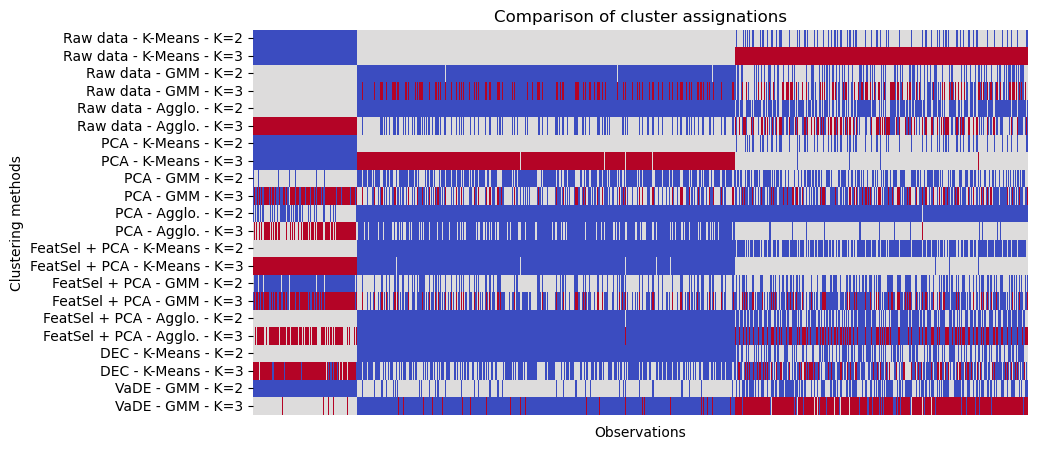
\includegraphics[width=\textwidth]{private_dataset/cluster_heatmap/clusters.png}
            \caption[Comparació dels clústers pel conjunt de dades DCH-NG]{
                Comparació dels clústers trobats pels diferents mètodes avaluats
                sobre el conjunt de dades \gls{privades}.
            }
            \label{f:dchng_heatmap}
        \end{figure}

        \begin{figure}[p]
            \centering
            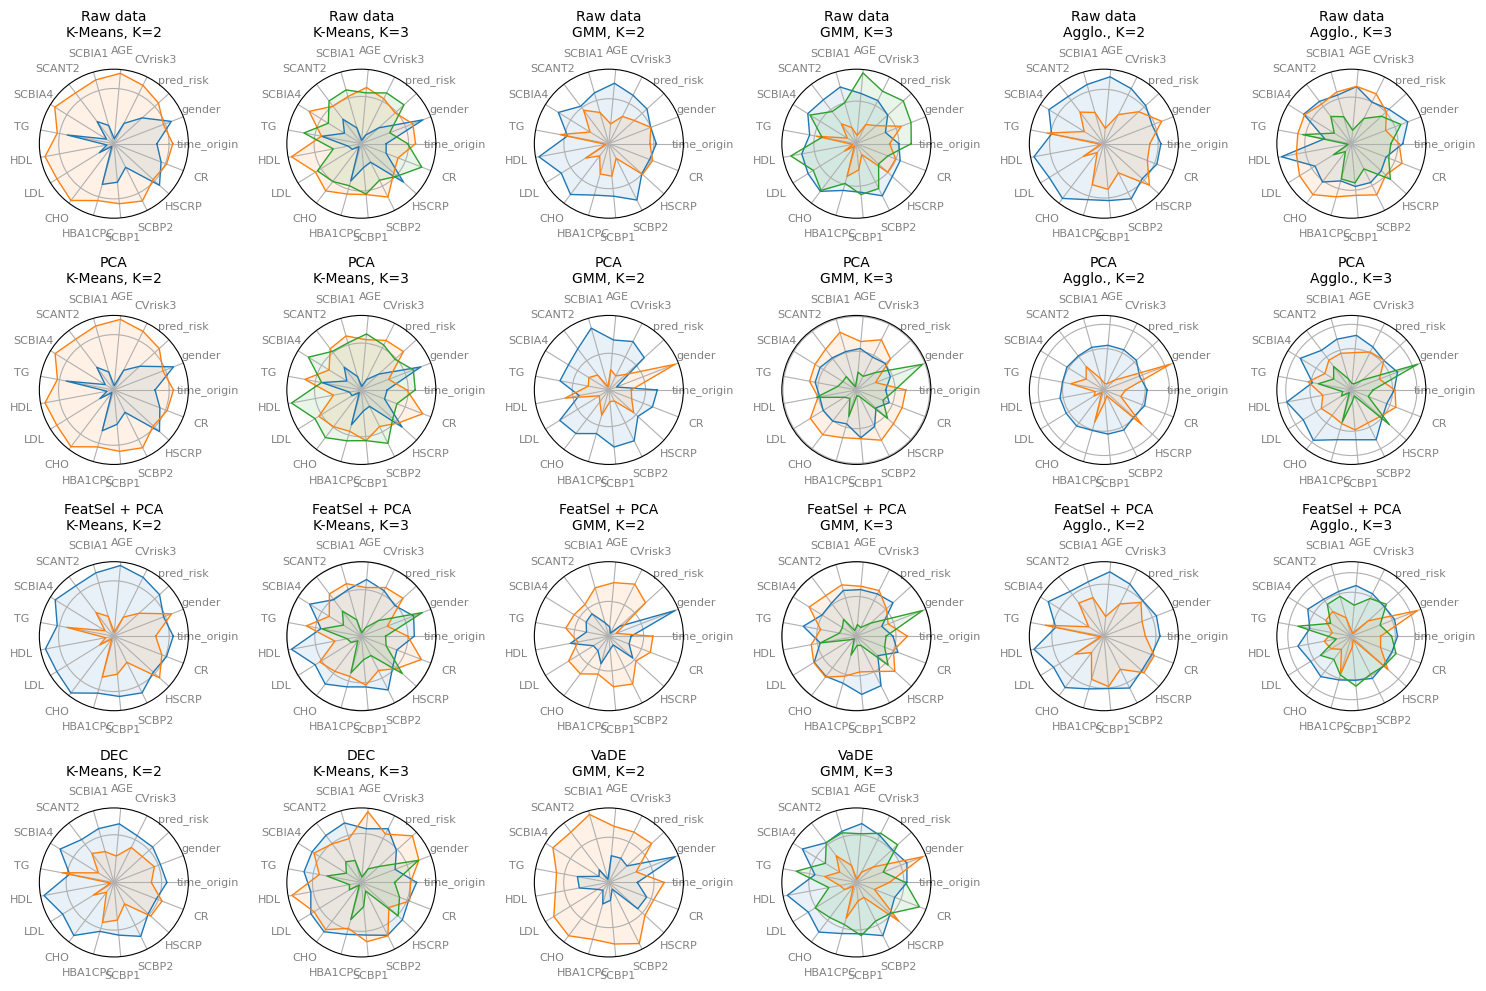
\includegraphics[width=\textwidth]{private_dataset/radialplots/covariates.png}
            \caption[Distribució diferencial de les covariables a DCH-NG]{
                Representació de la distribució diferencial
                de les covariables del conjunt de dades \gls{privades}
                en funció dels clústers trobats pels diferents mètodes avaluats.
            }
            \label{f:dchng_radial_covars}
        \end{figure}

        \begin{figure}[p]
            \centering
            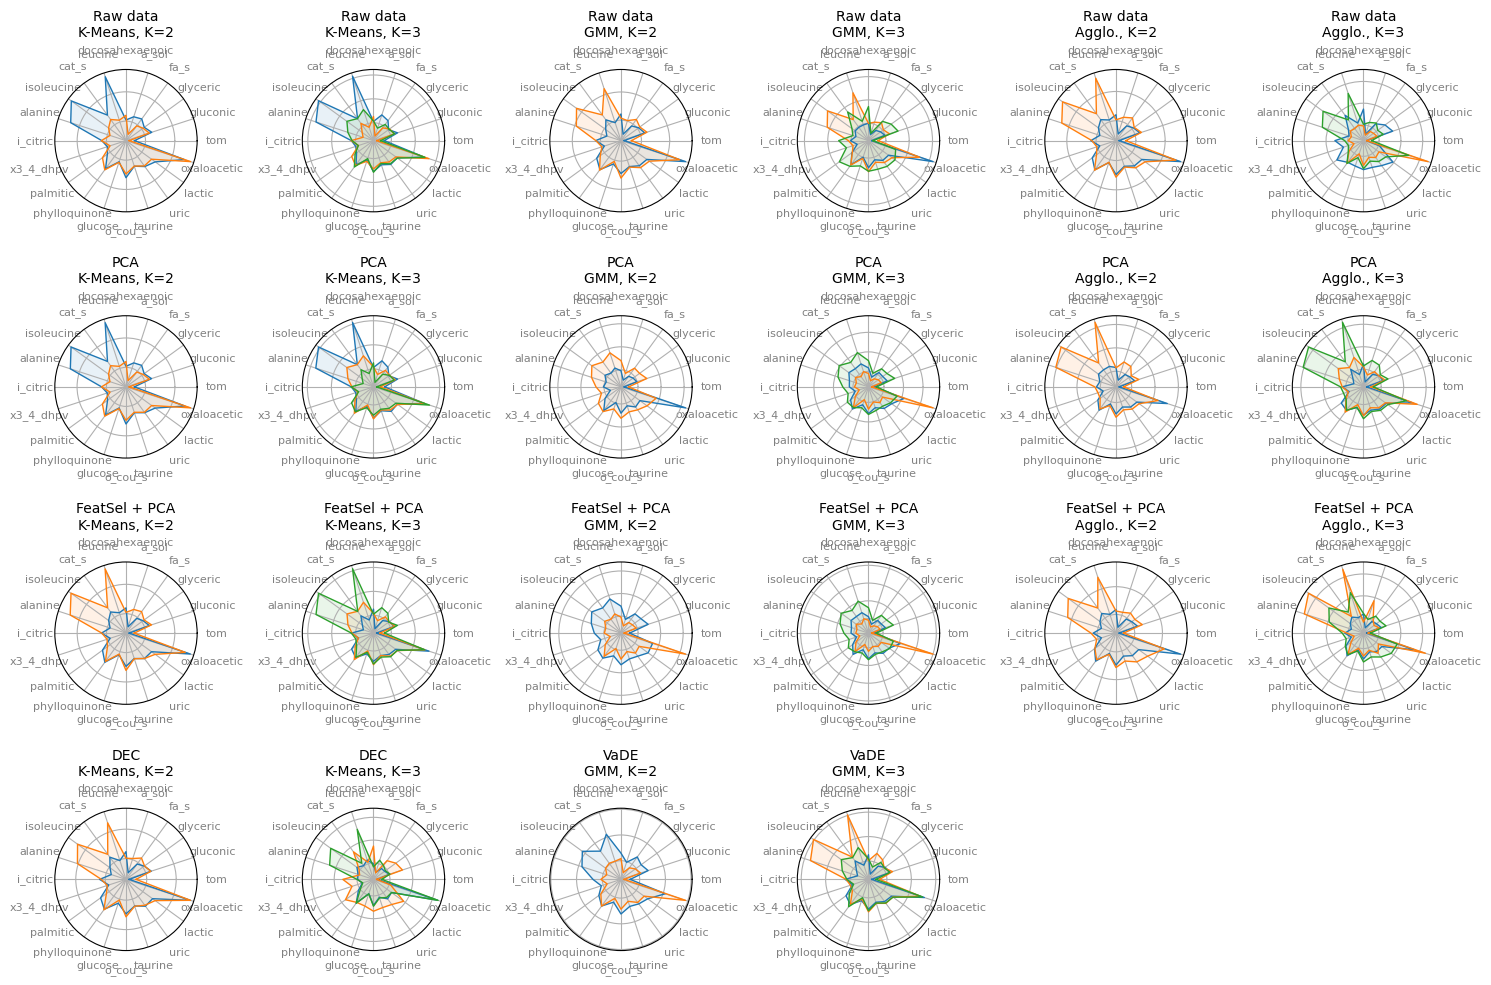
\includegraphics[width=\textwidth]{private_dataset/radialplots/most_var_feat.png}
            \caption[Distribució diferencial dels 20 metabòlits amb més variància a DCH-NG]{
                Representació de la distribució diferencial
                dels metabòlits amb més variància del conjunt de dades \gls{privades}
                en funció dels clústers trobats pels diferents mètodes avaluats.
            }
            \label{f:dchng_radial_mostvar}
        \end{figure}


        \begin{sidewaystable}[p]
            \small
            \centering
            \begin{tabular}{@{}lllllllllll@{}}
                \toprule
                \textbf{Tipus} & \textit{\textbf{Feature learning}} & \textit{\textbf{Clustering}} & \textbf{Inicialització} & \textbf{\begin{tabular}[c]{@{}l@{}}Núm.\\ clústers\end{tabular}} & \textbf{\begin{tabular}[c]{@{}l@{}}Covariable\\ referència\end{tabular}} & \textbf{\gls{acc}} & \textbf{\gls{ari}} & \textbf{\gls{ami}} & \textbf{\gls{sil}} & \textbf{\begin{tabular}[c]{@{}l@{}}Mateix\\ clúst.\end{tabular}} \\ \midrule
                \multirow{18}{*}{Clàssic} & \multirow{6}{*}{-} & \multirow{2}{*}{K-Means} & - & 2 & gender & 0.55 & 0 & 0 & 0.25 & 0.47 \\
                &  &  & - & 3 & CVrisk3 & 0.36 & 0 & 0 & 0.09 & 0.21 \\
                &  & \multirow{2}{*}{GMM} & - & 2 & gender & 0.55 & 0 & 0 & 0.17 & 0.33 \\
                &  &  & - & 3 & CVrisk3 & 0.36 & 0 & 0 & 0.1 & 0.17 \\
                &  & \multirow{2}{*}{Agglo.} & - & 2 & gender & 0.55 & 0 & 0 & 0.24 & 0.46 \\
                &  &  & - & 3 & CVrisk3 & 0.36 & 0 & 0 & 0.11 & 0.18 \\
                & \multirow{6}{*}{PCA} & \multirow{2}{*}{K-Means} & - & 2 & gender & 0.55 & 0 & 0 & 0.29 & 0.47 \\
                &  &  & - & 3 & CVrisk3 & 0.36 & 0 & 0 & 0.12 & 0.2 \\
                &  & \multirow{2}{*}{GMM} & - & 2 & gender & 0.55 & 0.01 & 0.01 & 0.14 & 0.24 \\
                &  &  & - & 3 & CVrisk3 & 0.37 & 0 & 0 & 0.02 & 0.12 \\
                &  & \multirow{2}{*}{Agglo.} & - & 2 & gender & 0.55 & 0 & 0 & 0.38 & 0.75 \\
                &  &  & - & 3 & CVrisk3 & 0.35 & 0 & 0 & 0.1 & 0.24 \\
                & \multirow{6}{*}{\begin{tabular}[c]{@{}l@{}}Selecció \\ de variables\\ +\\ PCA\end{tabular}} & \multirow{2}{*}{K-Means} & - & 2 & gender & 0.55 & 0 & 0 & 0.32 & 0.48 \\
                &  &  & - & 3 & CVrisk3 & 0.36 & 0 & 0 & 0.14 & 0.2 \\
                &  & \multirow{2}{*}{GMM} & - & 2 & gender & 0.55 & 0.01 & 0.01 & 0.16 & 0.25 \\
                &  &  & - & 3 & CVrisk3 & 0.36 & 0 & 0 & 0.02 & 0.14 \\
                &  & \multirow{2}{*}{Agglo.} & - & 2 & gender & 0.55 & 0 & 0 & 0.28 & 0.41 \\
                &  &  & - & 3 & CVrisk3 & 0.36 & 0 & 0 & 0.22 & 0.39 \\
                \multirow{4}{*}{\textit{\begin{tabular}[c]{@{}l@{}}Deep\\ clustering\end{tabular}}} & \multirow{2}{*}{DEC} & DEC & K-Means & 2 & gender & 0.55 & 0 & 0 & 0.96 & 0.35 \\
                &  & DEC & K-Means & 3 & CVrisk3 & 0.36 & 0 & 0 & 0.93 & 0.15 \\
                & \multirow{2}{*}{VaDE} & VaDE & GMM & 2 & gender & 0.55 & 0 & 0 & 0.57 & 0.3 \\
                &  & VaDE & GMM & 3 & CVrisk3 & 0.36 & 0 & 0 & 0.45 & 0.2 \\ \bottomrule
            \end{tabular}
            \caption[Dades DCH-NG: resultats]{Resum dels resultats obtinguts sobre el cojunt de dades metabolòmiques \gls{privades}.
            \textit{(Mateix clust.: freqüència amb que les observacions del mateix individu
            s'assignen a un únic clúster (corregida per la mida del clúster))}}
            \label{t:dadespriv_results}
        \end{sidewaystable}






\chapter{Discussió}
\label{c:discussio}
    %Discussió dels resultats en el context del projecte. És en aquest apartat on cobren sentit i en el qual es responen les preguntes de recerca i es mostra com els resultats donen resposta als problemes plantejats.
    %Aquesta part pot ser que no apliqui segons el tipus de treball.

    Els resultats obtinguts amb les dades \gls{mnist}
    mostren que els models de \textit{deep clustering}
    obtenen en general millor \gls{qc} que les tècniques clàssiques.
    Això suggereix que són capaços d'aprendre \gls{lf} més eficients
    degut a la seva capacitat de trobar relacions no lineals.

    El model \gls{dec} obté uns clústers molt similars
    als aconseguits aplicant tècniques clàssiques a la \gls{cr} d'un \gls{ae},
    però aconsegueix millor \gls{qc}.
    Els models basats en \gls{vae} no aconsegueixen un bon rendiment.

    Els models que han obtingut millor rendiment
    són els \gls{dec} i \gls{vade}.
    La resta de models s'han descartat
    de la resta de l'estudi.


    \paragraph{Model \gls{dec}}
        El model \gls{dec} ha aconseguit generar
        els clústers amb millors puntuacions per la mètrica silueta,
        amb diferència.
        Això indica que la \gls{cr} té una gran capacitat
        de separar les observacions en funció dels clústers aconseguits.

        Per altra banda,
        aquest model mostra ser especialment sensible
        als paràmetres amb que s'inicialitza.
        En conseqüència,
        el seu rendiment depèn de que les \gls{lf} apreses durant la fase de pre-entrenament
        propiciïn una bona \gls{qc} amb els mètodes clàssics
        utilitzats per inicialitzar els paràmetres.

        Durant la fase d'ajustament del model,
        s'accentua el criteri utilitzat per separar els clústers inicials,
        de manera que no s'obté nova informació,
        però s'aconsegueixen clústers més comprimits,
        resultant en una millor \gls{qc}.


    \paragraph{Model \gls{vae}}
        La principal característica del model \gls{vae}
        és que la seva \gls{cr} es basa en un model probabilístic
        i per tant no determina punts fixos en un espai dimensional,
        sinó els paràmetres d'una distribució normal multivariant
        de la qual es mostregen punts aleatoris.
        Això aconsegueix que la \gls{cr} sigui contínua
        i per tant pugui funcionar com un model generatiu,
        mostrejant punts de la distribució latent
        i passant-los al descodificador
        per obtenir una nova observació artificial
        que hauria de compartir la distribució de les variables originals.

        S'ha trobat que els models basats en \gls{vae}
        no aconsegueixen una bona \gls{qc}.
        Això és degut a l'aleatorietat del model probabilístic
        i el fet que tots els punts comparteixin la mateixa distribució latent.
        En conseqüència,
        encara que el model pugui ser capaç de diferenciar grups,
        és difícil aconseguir clústers que no presentin solapament.

        Aquesta idea queda il·lustrada a la \cref{f:vaedec_comp},
        on es comparen els models VAE+DEC que mantenen o descarten el descodificador:
        el model que el manté el descodificador,
        i per tant manté la funció de cost de regularització durant l'entrenament
        obté clústers molt més laxos i que presenten major solapament
        (el que es tradueix en puntuacions més baixes per la mètrica silueta)
        en comparació amb el model que descarta el descodificador,
        i per tant s'entrena únicament amb la funció de cost de \textit{clustering}.

        Aquest problema es pot entendre
        des d'un punt de vista de les funcions de cost,
        utilitzades per entrenar el model.
        El model VAE+DEC que manté el descodificador,
        durant l'entrenament se li aplica una funció de cost
        que es pot dividir en tres parts:
        funció de cost de reconstrucció,
        de regularització
        i de clustering.

        La funció de cost de regularització
        minimitza la distància de la distribució obtinguda a la capa latent
        amb la distribució objectiu (normal multivariant),
        mentre que la funció de cost de \textit{clustering}
        minimitza la distància de cada punt al centroide del seu clúster,
        alhora que maximitza la distància als centroides de la resta de clústers.
        Al maximitzar la distància entre centroides,
        la distribució s'allunya d'una distribució normal,
        i viceversa.
        En conseqüència, minimitzar una funció de cost penalitza a l'altra
        i el model resultat no aconsegueix optimitzar cap de les dues.


    \paragraph{Model \gls{vae}}

        El model \gls{vade} resol aquest problema
        assignant una distribució independent a cada grup.
        D'aquesta manera,
        augmentar la distància entre clústers
        no penalitza a la funció de regularització
        i es poden optimitzar les dues simultàniament.

        Així, s'obté un model de \textit{deep clustering}
        que manté la capacitat generativa del model \gls{vae}.
        A la \cref{f:vaevadedec_comp} es mostra gràficament
        la diferència entre les representacions obtingudes pels dos models
        sobre les dades \gls{mnist}.

        No s'han explorat les característiques generatives
        del model \gls{vade},
        que juntament amb la seva capacitat d'obtenir una bona \gls{qc}
        el converteixen en un model interessant.

        \begin{figure}
            \centering
            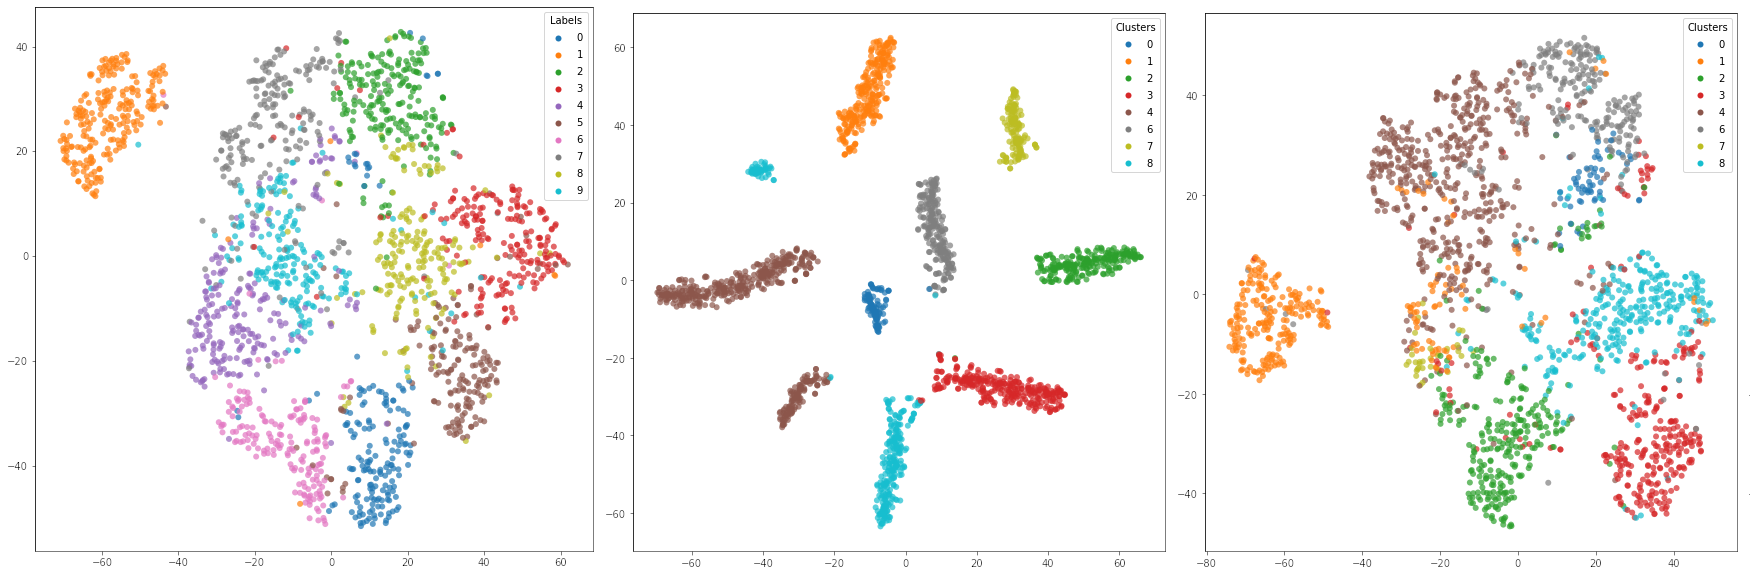
\includegraphics[width=\textwidth]{mnist/tsne_embeddings/vaedec_comparison.png}
            \caption[Comparació dels models VAE+DEC]{
                Comparació dels models VAE+DEC.
                Representació \gls{tsne} de la \gls{cr} del model \gls{vae} pre-entrenat (\textbf{esquerra}),
                del model combinat que perd el descodificador (\textbf{centre})
                i del model combinat que manté el descodificador (\textbf{dreta}).
                S'observa una clara millora en la \gls{qc} obtinguda pel model que perd el descodificador.
            }
            \label{f:vaedec_comp}
        \end{figure}


    \paragraph{Dades metabolòmiques i interpretació biològica}
        Al aplicar les tècniques sobre les dades metabolòmiques,
        el rendiment de les tècniques de \textit{deep clustering}
        no sembla millorar respecte a les tècniques clàssiques.
        Segurament això és degut a que aquestes dades presenten
        una estructura molt més complexa
        que és difícil de modelar inclús pels models de \textit{deep clusteirng}.

        A més, per la seva naturalesa es disposa d'un número de dades molt més petit
        que els que es solen utilitzar per entrenar models de \textit{deep learning},
        com per exemple les dades \gls{mnist}.
        Això a provocat també la mida dels models implementats
        s'hagin acotat molt,
        limitant així la seva capacitat d'aprenentatge.

        S'ha observat que els clústers trobats per les diferents tècniques
        (i números de clústers)
        presenten en general un bon solapament,
        és a dir que agrupen les observacions de manera similar.
        Això seria indicatiu de que existeix algun tipus d'estructura latent a les dades.

        La major dificultat s'ha presentat
        alhora de donar una interpretació als grups trobats,
        donat que presenten distribucions multivariants complexes.
        Encara que les dades \gls{privades} mostren
        uns resultats que apunten a una possible interpretació biològica,
        seria necessari un estudi addicional per confirmar-ho.

        Un estudi més profund d'aquestes distribucions
        podria ajudar a trobar un criteri més clar
        amb el que valorar l'efectivitat de les diferents tècniques.

        Per tant,
        es considera que des del punt de vista de la interpretació biològica
        els resultats són poc concloents
        i requeririen un estudi més profund.



\chapter{Valoració econòmica}
\label{c:economic}
    %En cas que correspongui, s'inclourà un apartat de ``Valoració econòmica del treball". Aquest apartat indicarà les despeses associades al desenvolupament i manteniment del treball, així com els beneficis econòmics obtinguts. Cal fer una anàlisi final sobre la viabilitat del producte.

    La realització d'aquest \gls{tfm} ha requerit d'una única despesa econòmica:
    una subscripció Paperspace Gradient,
    el servei de computació \textit{on-line}
    que es menciona a la \cref{s:software}.

    Encara que aquesta plataforma ofereix un servei gratuït,
    s'ha considerat insuficient
    ja que no garanteix la disponibilitat de màquines virtuals en qualsevol moment.

    S'ha subscrit el pla de pagament més econòmic,
    que ha cobert els requisits de poder de computació
    i disponibilitat.
    La subscripció ha tingut un cost de \$8 al mes
    i s'ha activat durant els mesos de novembre, desembre i generdurant,
    sumant per tant un total de \$24
    (equivalent a aproximadament 22 € en el moment de redactar aquest informe).

    Aquest servei només ha sigut necessari
    ja que no es disposa d'una màquina prou potent
    per entrenar els models neuronals que s'han implementat.

    Donat que el cost mensual d'aquest servei és petit,
    que no és estrictament necessari
    si es disposa d'una màquina suficientment potent,
    i que l'objectiu no ha sigut desenvolupar un producte econòmicament sostenible,
    si no implementar i avaluar una sèrie de models prototip,
    es considera que el cost ha sigut perfectament assumible.


\chapter{Conclusions i treballs futurs}
\label{c:conclusions}

    \section{Conclusions}
    \label{s:conclusions}
        %Aquest capítol ha d'incloure:
        %\begin{itemize}
        %    \item Una descripció de les conclusions del treball:
        %    \begin{itemize}
        %        \item Un cop s’han obtingut els resultats quines conclusions s’extreu?
        %        \item Aquests resultats són els esperats? O han estat sorprenents? Per què?
        %    \end{itemize}
        %    \item Una reflexió crítica sobre l’assoliment dels objectius plantejats inicialment:
        %    \begin{itemize}
        %        \item Hem assolit tots els objectius? Si la resposta és negativa, per quin motiu?
        %    \end{itemize}
        %\end{itemize}

        De manera sintetitzada,
        les conclusions que s'han extret en aquest \gls{tfm} són:

        \begin{itemize}
            \item Els models de \textit{deep clustering}
            tenen la capacitat de superar el rendiment de les tècniques clàssiques,
            a costa d'un augment significatiu de la complexitat del model.

            \item El model \gls{dec} destaca per aconseguir clústers molt estrets,
            però és molt sensible als paràmetres amb què s'inicialitza.

            \item El model \gls{vade} aconsegueix una bona \gls{qc},
            i a més té la capacitat de funcionar com un model generatiu.

            \item L'arquitectura \gls{vae} no propicia una bona \gls{qc}
            donat que la \gls{cr} està acotada a una única distribució latent,
            compartida per totes les observacions.

            \item Tots els mètodes avaluats sobre les dades metabolòmiques
            (\gls{kmeans}, \gls{gmm}, \gls{aglo}, \gls{dec}, \gls{vade})
            mostren un alt nivell de solapament dels clústers trobats.
            És a dir, troben una estructura latent de les dades similar.

            \item Encara que els clústers obtinguts
            mostren certes diferències en la distribució multivariant
            de les covariables d'interès,
            la seva interpretació és complexa
            i requeriria d'un estudi posterior.
        \end{itemize}

        Els resultats obtinguts es consideren satisfactoris
        i es considera que s'han aconseguit els objectius inicials.

        La implementació dels models de \textit{deep learning}
        he resultat una tasca més complicada del que s'esperava,
        però finalment s'ha aconseguit.

        El temps disponible per realitzar aquest \gls{tfm}
        ha fet necessari limitar l'anàlisi que s'ha fet dels resultats obtinguts.
        A la següent secció es presenten una sèrie de idees
        que no ha donat temps d'estudiar.



    \section{Línies de futur}
    \label{s:futur}
        %Les línies de treball futur que no s'han pogut explorar en aquest treball i han quedat pendents.

        Durant el desenvolupament d'aquest \gls{tfm}
        han sorgit diverses idees que no s'han pogut explorar
        donada la limitació de temps disponible.

        Algunes d'aquestes idees es podrien desenvolupar
        en estudis posteriors.
        Es fan les següents propostes:

        \paragraph{Dades \gls{privades}}
            En l'estudi del conjunt de dades \gls{privades}
            no s'ha tingut en compte que es tracta de mesures repetides en el temps.
            Concretament,
            es disposa de tres mesures realitzades sobre els mateixos individus.

            Es proposa estudiar les tècniques de \textit{deep clustering} avaluades,
            entrenant els models amb les dades d'un dels temps
            i avaluant els resultats amb les dades dels altres dos temps.
            Fent el mateix per els altres dos grups,
            es pot realitzar validació creuada.

            Una segona proposta és separar les dades en tres subconjunts en funció del temps,
            aplicar les tècniques de \textit{clustering} sobre cada subconjunt per separat
            i comparar les assignacions obtingudes.
            S'esperaria observar major variació entre individus
            que entre les observacions del mateix individu.
            Per tant, s'esperaria que trobar un fort solapament entre els clústers:
            el mateix individu s'hauria d'assignar al mateix clúster en els diferents temps.

            Per últim,
            es proposa estudiar la interpretació biològica dels clústers obtinguts
            mitjançant un estudi multivariant per mesures repetides.

        \paragraph{Exposome Data Challenge Event}
            Es tracta d'un conjunt de dades molt complexe
            compost per dades de diversos orígens,
            pel que les possibilitats d'estudi són molt àmplies.

            Una aproximació que no s'ha realitzat en aquest \gls{tfm}
            per falta de temps és
            implementar un model basat en un \gls{ae}
            que tingui dues entrades.
            El model es compondria per dos (o múltiples) codificadors paral·lels.
            Les capes de representació es combinarien concatenant
            les respectives capes neuronals,
            i posteriorment es podria aplicar \textit{clustering}
            mitjançant tècniques clàssiques o un model \gls{dec}.

            Cada un dels codificadors tindrien com entrada un subconjunt de dades,
            per exemple les dades metabolòmiques de sèrum i d'orina,
            les dades metabolòmiques i les dades del exposoma,
            o algun dels subconjunts de dades òmiques i un dels subconjunts de covariables.
            D'aquesta manera es podria obtenir informació sobre una estructura latent
            condicionada simultàniament a diversos conjunts de dades.

            Els codificadors es podrien aconseguir entrenant dos \gls{ae} per separat,
            i després unint-los,
            o implementant directament un \gls{ae} amb dues entrades i dues sortides.

        \paragraph{Models generatius}
            Els models \gls{vae} i \gls{vade} es caracteritzen
            per la seva capacitat generativa:
            es poden generar noves dades artificials
            prenent mostres de la distribució de la seva capa latent
            i passant-les pel descodificador del model.

            Donat que una de les limitacions de les dades metabolòmiques
            (i òmiques en general)
            és que solen tenir un número reduït de mostres,
            es proposa estudiar la viabilitat d'utilitzar aquests models
            com a tècnica d'augment de les dades,
            ja sigui per realitzar estudis de \textit{clustering}
            o aplicar altres mètodes d'anàlisi.

        \paragraph{Model barreja d'experts}
            Una altra idea que no ha donat temps d'estudiar en aquest \gls{tfm}
            és desenvolupar un model tipus \textit{mixture of experts}.
            Un cop implementats i seleccionats els models individuals de \textit{clustering},
            es podria aplicar un mètode per unificar les assignacions
            de clústers a un sol criteri.

            Això podria realitzar-se de manera més o menys senzilla,
            assignant a cada observació el clúster que mostri més solapament
            entre les diferents tècniques,
            o mitjançant una xarxa neuronal més complexa
            que combini els diversos models en una sola sortida.

        \paragraph{Interpretació dels clústers}
            En aquest \gls{tfm} no s'ha estudiat amb profunditat
            la possible interpretació biològica dels clústers.
            Es proposa realitzar un estudi més rigorós
            analitzant la distribució multivariant diferencial en funció dels clústers obtinguts.

        \paragraph{Número de clústers}
            Per últim,
            es planteja una limitació important de totes les tècniques avaluades
            en aquest \gls{tfm}:
            la selecció d'un nombre de clústers òptim.

            Excepte el mètode aglomeratiu,
            tots els mètodes utilitzats requereixen fixar prèviament un nombre de clústers.
            Sovint no és factible conèixer el número de clústers per endavant,
            precisament perquè l'objectiu de les tècniques de \textit{clustering}
            és buscar una estructura latent desconeguda.

            En aquest sentit, s'ha de manera superficial l'eina \textit{clValid}\footnote{https://www.rdocumentation.org/packages/clValid/versions/0.7/topics/clValid},
            un paquet de R que permet avaluar simultàniament
            diverses tècniques de \textit{clustering} clàssiques
            mesurant diferents mètriques internes, d'estabilitat i biològiques.

            Es proposa estudiar el conjunt de dades Exposome Data Challenge Event
            amb l'objectiu de trobar un número de clústers òptim
            que admeti la seva interpretació.
            Posteriorment es podria tornar a avaluar els diferents mètodes
            en funció del seu alineament amb aquesta interpretació.


    \section{Seguiment de la planificació}
    \label{s:seguiment}
        %\begin{itemize}
        %    \item Una anàlisi crítica del seguiment de la planificació i metodologia al llarg del producte:
        %    \begin{itemize}
        %        \item S’ha seguit la planificació?
        %        \item La metodología prevista ha estat prou adequada?
        %        \item Ha calgut introduir canvis per garantir l’èxit del treball? Per què?
        %    \end{itemize}
        %    \item Dels impactes previstos a \ref{s:etic}, ètic-socials, de sostenibilitat i de diversitat, avaluaeu/esmenteu si s'han mitigat (si eren negatius) o si s'han aconseguit (si eren positius).
        %    \item Si han aparegut impactes no previstos a \ref{s:etic}, avaluar/esmentar com s'han mitigat (si eren negatius) o què han aportat (si eren positius).
        %\end{itemize}


        Si bé es considera que s'han complert tots els objectius
        globals i específics
        especificats a l'inici del projecte,
        no s'han respectat les dates del pla de treball.
        Això ha estat causat per dos motius.

        \paragraph{Compaginar recerca teòrica i treball pràctic}
            La fase inicial del \gls{tfm},
            en la que es pretenia obtenir una base sòlida de coneixements
            teòrics i pràctics
            sobre la que desenvolupar la resta del treball,
            es va definir inicialment com un bloc
            independent de la resta del projecte.

            A mesura que es va anar avançant,
            i sobretot després de fer les primeres proves
            d'implementar xarxes neuronals amb certa complexitat amb Keras,
            es va trobar més productiu compaginar
            les tasques de formació
            amb la implementació de les primeres versions
            dels models de \textit{deep clustering}.
            Realitzar aquestes dues tasques
            de manera simultània va ajudar a consolidar els coneixements
            teòrics i pràctics,
            i a trobar limitacions dels models que no s'havia tingut en compte inicialment.

            Això va tenir l'efecte que,
            per una banda,
            s'endarrerís el compliment del primer objectiu específic,
            alhora que es va avançar l'inici del segon.

        \paragraph{Augment de complexitat del problema}
            Inicialment,
            aquest \gls{tfm} es va titular
            \textit{Desenvolupament d’un model de \textit{deep clustering}
            en dades metabolòmiques
            utilitzant un Variational Autoencoder},
            ja que en una primera presa de contacte amb la literatura
            es va pensar que el \gls{vae},
            degut a la seva capacitat com a model generatiu,
            podia ser una base interessant
            sobre la que construir un model de \textit{deep clustering}.

            Si bé la idea no estava equivocada
            (el model \gls{vade} parteix precisament d'aquest concepte),
            la implementació que es va intentar inicialment
            va resultar problemàtica.

            Un cop entès el funcionament de l'arquitectura \gls{vae},
            i després d'implementar un model i comprovar el seu correcte funcionament,
            es va procedir a afegir al model una capa de \textit{clustering}
            similar al model mixte \gls{vae} + \gls{dec}
            que es va avaluar amb el conjunt de dades \gls{mnist}.

            Finalment es va comprendre que aquest model
            no és adequat per realitzar aquesta tasca,
            com s'explica al \cref{c:discussio}.

            En resposta a aquest problema,
            es van estudiar i implementar dos models de \textit{deep clustering}
            addicionals: \gls{dec} i \gls{vade},
            el que va suposar una dedicació extra.

            Tot això va portar a canviar lleugerament
            la direcció del \gls{tfm}:
            en lloc d'implementar un model \gls{vae}
            per realitzar \textit{clustering}
            en dades metabolòmiques,
            s'han implementat diversos models i s'han comparat els resultats obtinguts.

            La conseqüència negativa més significativa
            és que no s'ha disposat del temps que s'hauria desitjat
            per analitzar més detingudament els resultats
            i obtenir unes conclusions més interessants.


% GLOSSARI
\printglossary[type=\acronymtype, title={Glossari i abreviacions}]

% BIBLIOGRAFIA
%\chapter{Bibliografia} %\bibliography{} ja afegeix el \chapter{} corresponent!
\bibliographystyle{ieeetr}
\bibliography{TFM, TFM-software}

\chapter*{Agraïments}

    M'agradaria expressar el meu agraïment a Esteban Vegas Lozano,
    el meu tutor en aquest \gls{tfm},
    pel temps dedicat a llegir esborranys de la memòria
    i els meus e-mails amb múltiples capítols,
    així com pel suport que m'ha donat aportant idees molt valuoses
    i tranquil·litzant-me en els moments complicats
    en que els resultats no semblaven sortir.

    També vull agrair a l'equip de recerca
    \textit{Biomarkers and Nutritional \& Food Metabolomics}
    del Departament de Nutrició, Ciències de l'Alimentació i Gastronomia
    de la Universitat de Barcelona
    que hagi compartit desinteressadament el conjunt de dades \gls{privades}.

\newpage
\appendix
%Llistat d’apartats que són massa extensos per incloure dins la memòria i tenen un caràcter autocontingut (per exemple, manuals d’usuari, manuals d’instal·lació, etc.)
%Depenent del tipus de treball, és possible que no calgui afegir cap annex.

\chapter{Exposome Data Challenge Event: resultats complets}
\label{a:exposome}

    \section{Taules de mètriques}

    En les següents pàgines es mostren els resultats complets
    de les mètriques mesurades en el conjunt de dades
    Exposome Data Challenge Event.

    %    \setlength\arrayrulewidth{1pt}
    \begin{table}
        \scriptsize
        \centering
        \begin{tabular}{@{}ccccccccc@{}}
            \toprule
            \textit{\textbf{Feature learning}} & \textit{\textbf{Clustering}} & \textbf{Inicialització} & \textbf{\begin{tabular}[c]{@{}l@{}}Núm.\\ clústers\end{tabular}} & \textbf{\begin{tabular}[c]{@{}l@{}}Covariable\\ referència\end{tabular}} & \textbf{\gls{acc}} & \textbf{\gls{ari}} & \textbf{\gls{ami}} & \textbf{\gls{sil}} \\ \midrule
            \multirow{30}{*}{-} & \multirow{10}{*}{K-Means} & \multirow{10}{*}{-} & 2 & asthma & 0.89 & 0 & 0 & 0.1 \\
            &  &  & 2 & sex & 0.53 & 0 & 0 & 0.1 \\
            &  &  & 3 & education & 0.51 & 0 & 0 & 0.07 \\
            &  &  & 3 & native & 0.84 & 0 & 0 & 0.07 \\
            &  &  & 3 & parity & 0.45 & 0 & 0 & 0.07 \\
            &  &  & 4 & birth\_weight & 0.27 & 0 & 0 & 0.06 \\
            &  &  & 4 & iq & 0.3 & 0 & 0 & 0.06 \\
            &  &  & 4 & behaviour & 0.27 & 0 & 0 & 0.06 \\
            &  &  & 6 & cohort & 0.21 & 0 & 0 & 0.05 \\
            &  &  & 7 & age & 0.32 & 0 & 0 & 0.05 \\ \cmidrule(l){2-9}
            & \multirow{10}{*}{GMM} & \multirow{10}{*}{-} & 2 & asthma & 0.89 & 0 & 0 & 0.1 \\
            &  &  & 2 & sex & 0.53 & 0 & 0 & 0.1 \\
            &  &  & 3 & education & 0.51 & 0 & 0 & 0.06 \\
            &  &  & 3 & native & 0.84 & 0 & 0 & 0.06 \\
            &  &  & 3 & parity & 0.45 & 0 & 0 & 0.06 \\
            &  &  & 4 & birth\_weight & 0.27 & 0 & 0 & 0.06 \\
            &  &  & 4 & iq & 0.3 & 0 & 0 & 0.06 \\
            &  &  & 4 & behaviour & 0.27 & 0 & 0 & 0.06 \\
            &  &  & 6 & cohort & 0.22 & 0 & 0 & 0.04 \\
            &  &  & 7 & age & 0.32 & 0 & 0 & 0.04 \\ \cmidrule(l){2-9}
            & \multirow{10}{*}{Agglo.} & \multirow{10}{*}{-} & 2 & asthma & 0.89 & 0 & 0 & 0.09 \\
            &  &  & 2 & sex & 0.53 & 0 & 0 & 0.09 \\
            &  &  & 3 & education & 0.51 & 0 & 0 & 0.05 \\
            &  &  & 3 & native & 0.84 & 0 & 0 & 0.05 \\
            &  &  & 3 & parity & 0.46 & 0 & 0 & 0.05 \\
            &  &  & 4 & birth\_weight & 0.27 & 0 & 0 & 0.04 \\
            &  &  & 4 & iq & 0.3 & 0 & 0 & 0.04 \\
            &  &  & 4 & behaviour & 0.27 & 0 & 0 & 0.04 \\
            &  &  & 6 & cohort & 0.21 & 0 & 0 & 0.02 \\
            &  &  & 7 & age & 0.32 & 0 & 0 & 0.02 \\ \midrule
            \multirow{30}{*}{PCA} & \multirow{10}{*}{K-Means} & \multirow{10}{*}{-} & 2 & asthma & 0.89 & 0 & 0 & 0.13 \\
            &  &  & 2 & sex & 0.53 & 0 & 0 & 0.13 \\
            &  &  & 3 & education & 0.51 & 0 & 0 & 0.08 \\
            &  &  & 3 & native & 0.84 & 0 & 0 & 0.08 \\
            &  &  & 3 & parity & 0.45 & 0 & 0 & 0.08 \\
            &  &  & 4 & birth\_weight & 0.27 & 0 & 0 & 0.08 \\
            &  &  & 4 & iq & 0.3 & 0 & 0 & 0.08 \\
            &  &  & 4 & behaviour & 0.27 & 0 & 0 & 0.08 \\
            &  &  & 6 & cohort & 0.22 & 0 & 0 & 0.06 \\
            &  &  & 7 & age & 0.32 & 0 & 0 & 0.06 \\ \cmidrule(l){2-9}
            & \multirow{10}{*}{GMM} & \multirow{10}{*}{-} & 2 & asthma & 0.89 & 0 & 0 & 0.02 \\
            &  &  & 2 & sex & 0.53 & 0 & 0 & 0.02 \\
            &  &  & 3 & education & 0.51 & 0 & 0 & 0.02 \\
            &  &  & 3 & native & 0.84 & 0 & 0 & 0.02 \\
            &  &  & 3 & parity & 0.45 & 0 & 0 & 0.02 \\
            &  &  & 4 & birth\_weight & 0.28 & 0 & 0 & 0 \\
            &  &  & 4 & iq & 0.32 & 0.01 & 0.01 & 0 \\
            &  &  & 4 & behaviour & 0.28 & 0 & 0 & 0 \\
            &  &  & 6 & cohort & 0.2 & 0 & 0 & -0.02 \\
            &  &  & 7 & age & 0.32 & 0 & 0 & -0.02 \\ \cmidrule(l){2-9}
            & \multirow{10}{*}{Agglo.} & \multirow{10}{*}{-} & 2 & asthma & 0.89 & 0 & 0 & 0.11 \\
            &  &  & 2 & sex & 0.53 & 0 & 0 & 0.11 \\
            &  &  & 3 & education & 0.51 & 0 & 0 & 0.06 \\
            &  &  & 3 & native & 0.84 & 0 & 0 & 0.06 \\
            &  &  & 3 & parity & 0.45 & 0 & 0 & 0.06 \\
            &  &  & 4 & birth\_weight & 0.27 & 0 & 0 & 0.05 \\
            &  &  & 4 & iq & 0.29 & 0 & 0 & 0.05 \\
            &  &  & 4 & behaviour & 0.27 & 0 & 0 & 0.05 \\
            &  &  & 6 & cohort & 0.2 & 0 & 0 & 0.03 \\
            &  &  & 7 & age & 0.32 & 0 & 0 & 0.03 \\ \bottomrule
        \end{tabular}
        \caption[Exposome Data Challenge Event: resultats - part 1]{
            Resultats obtinguts sobre el conjunt de dades Exposome Data Challenge Event
            (subcojunt metaboloma, dades originals, tècniques clàssiques).
        }
        \label{t:results_exposome1}
    \end{table}

    \newpage
    \scriptsize
    \begin{center}
        \begin{longtable}{@{}ccccccccc@{}}
            \toprule
            \textit{\textbf{Feature learning}} & \textit{\textbf{Clustering}} & \textbf{Inicialització} & \textbf{\begin{tabular}[c]{@{}l@{}}Núm.\\ clústers\end{tabular}} & \textbf{\begin{tabular}[c]{@{}l@{}}Covariable\\ referència\end{tabular}} & \textbf{\gls{acc}} & \textbf{\gls{ari}} & \textbf{\gls{ami}} & \textbf{\gls{sil}} \\ \hline
            \multirow{11}{*}{DEC} & \multirow{11}{*}{DEC} & \multirow{11}{*}{K-Means} & 2 & asthma & 0.89 & 0 & 0 & 0.7 \\
            &  &  & 2 & sex & 0.53 & 0 & 0 & 0.7 \\
            &  &  & 3 & education & 0.51 & 0 & 0 & 0.64 \\
            &  &  & 3 & native & 0.84 & 0 & 0 & 0.64 \\
            &  &  & 3 & parity & 0.45 & 0 & 0 & 0.64 \\
            &  &  & 4 & birth\_weight & 0.27 & 0 & 0 & 0.45 \\
            &  &  & 4 & iq & 0.29 & 0 & 0 & 0.45 \\
            &  &  & 4 & behaviour & 0.27 & 0 & 0 & 0.45 \\
            &  &  & 4 & bmi & 0.69 & 0 & 0 & 0.45 \\
            &  &  & 6 & cohort & 0.21 & 0 & 0 & 0.4 \\
            &  &  & 7 & age & 0.32 & 0 & 0 & 0.42 \\ \midrule
            \multirow{11}{*}{VaDE} & \multirow{11}{*}{VaDE} & \multirow{11}{*}{GMM} & 2 & asthma & 0.89 & 0 & 0 & 0.29 \\
            &  &  & 2 & sex & 0.53 & 0 & 0 & 0.29 \\
            &  &  & 3 & education & 0.51 & 0 & 0 & 0.16 \\
            &  &  & 3 & native & 0.84 & 0 & 0 & 0.16 \\
            &  &  & 3 & parity & 0.45 & 0 & 0 & 0.16 \\
            &  &  & 4 & birth\_weight & 0.28 & 0 & 0 & 0.15 \\
            &  &  & 4 & iq & 0.3 & 0 & 0 & 0.15 \\
            &  &  & 4 & behaviour & 0.27 & 0 & 0 & 0.15 \\
            &  &  & 4 & bmi & 0.69 & 0 & 0 & 0.15 \\
            &  &  & 6 & cohort & 0.21 & 0 & 0 & 0.11 \\
            &  &  & 7 & age & 0.32 & 0 & 0 & 0.09 \\ \midrule
            \multirow{11}{*}{DEC (D.A.)} & \multirow{11}{*}{DEC} & \multirow{11}{*}{K-Means} & 2 & asthma & 0.89 & 0 & 0 & 0.95 \\
            &  &  & 2 & sex & 0.53 & 0 & 0 & 0.95 \\
            &  &  & 3 & education & 0.51 & 0 & 0 & 0.91 \\
            &  &  & 3 & native & 0.84 & 0 & 0 & 0.91 \\
            &  &  & 3 & parity & 0.45 & 0 & 0 & 0.91 \\
            &  &  & 4 & birth\_weight & 0.27 & 0 & 0 & 0.77 \\
            &  &  & 4 & iq & 0.31 & 0.01 & 0 & 0.77 \\
            &  &  & 4 & behaviour & 0.3 & 0 & 0 & 0.77 \\
            &  &  & 4 & bmi & 0.69 & 0 & 0 & 0.77 \\
            &  &  & 6 & cohort & 0.2 & 0 & 0 & 0.77 \\
            &  &  & 7 & age & 0.32 & 0 & 0.01 & 0.71 \\ \midrule
            \multirow{11}{*}{VaDE (D.A.)} & \multirow{11}{*}{VaDE} & \multirow{11}{*}{GMM} & 2 & asthma & 0.89 & 0 & 0 & 0.35 \\
            &  &  & 2 & sex & 0.53 & 0 & 0 & 0.35 \\
            &  &  & 3 & education & 0.51 & 0 & 0 & 0.18 \\
            &  &  & 3 & native & 0.84 & 0 & 0 & 0.18 \\
            &  &  & 3 & parity & 0.47 & 0.01 & 0 & 0.18 \\
            &  &  & 4 & birth\_weight & 0.28 & 0 & 0 & 0.18 \\
            &  &  & 4 & iq & 0.31 & 0 & 0 & 0.18 \\
            &  &  & 4 & behaviour & 0.27 & 0 & 0 & 0.18 \\
            &  &  & 4 & bmi & 0.69 & 0 & 0 & 0.18 \\
            &  &  & 6 & cohort & 0.22 & 0 & 0 & 0.1 \\
            &  &  & 7 & age & 0.32 & 0 & 0 & 0.07 \\ \midrule
            \multirow{11}{*}{DEC (conv. 1D)} & \multirow{11}{*}{DEC} & \multirow{11}{*}{K-Means} & 2 & asthma & 0.89 & 0 & 0 & 0.64 \\
            &  &  & 2 & sex & 0.53 & 0 & 0 & 0.64 \\
            &  &  & 3 & education & 0.51 & 0 & 0 & 0.59 \\
            &  &  & 3 & native & 0.84 & 0 & 0 & 0.59 \\
            &  &  & 3 & parity & 0.45 & 0 & 0 & 0.59 \\
            &  &  & 4 & birth\_weight & 0.25 & 0 & 0 & 1 \\
            &  &  & 4 & iq & 0.28 & 0 & 0 & 1 \\
            &  &  & 4 & behaviour & 0.25 & 0 & 0 & 1 \\
            &  &  & 4 & bmi & 0.69 & 0 & 0 & 1 \\
            &  &  & 6 & cohort & 0.2 & 0 & 0 & 0.28 \\
            &  &  & 7 & age & 0.32 & 0 & 0 & 0.22 \\ \midrule
            \multirow{11}{*}{VaDE (conv. 1D)} & \multirow{11}{*}{VaDE} & \multirow{11}{*}{GMM} & 2 & asthma & 0.89 & 0 & 0 & 0.38 \\
            &  &  & 2 & sex & 0.53 & 0 & 0 & 0.38 \\
            &  &  & 3 & education & 0.51 & 0 & 0 & 0.2 \\
            &  &  & 3 & native & 0.84 & 0 & 0 & 0.2 \\
            &  &  & 3 & parity & 0.46 & 0 & 0 & 0.2 \\
            &  &  & 4 & birth\_weight & 0.27 & 0 & 0 & 0.18 \\
            &  &  & 4 & iq & 0.31 & 0.01 & 0 & 0.18 \\
            &  &  & 4 & behaviour & 0.27 & 0 & 0 & 0.18 \\
            &  &  & 4 & bmi & 0.69 & 0 & 0 & 0.18 \\
            &  &  & 6 & cohort & 0.21 & 0 & 0 & 0.12 \\
            &  &  & 7 & age & 0.32 & 0 & 0 & 0.09 \\ \midrule
            \multirow{11}{*}{DEC (conv. 2D)} & \multirow{11}{*}{DEC} & \multirow{11}{*}{K-Means} & 2 & asthma & 0.89 & 0 & 0 & 0.6 \\
            &  &  & 2 & sex & 0.53 & 0 & 0 & 0.6 \\
            &  &  & 3 & education & 0.51 & 0 & 0 & 0.56 \\
            &  &  & 3 & native & 0.84 & 0 & 0 & 0.56 \\
            &  &  & 3 & parity & 0.45 & 0 & 0 & 0.56 \\
            &  &  & 4 & birth\_weight & 0.27 & 0 & 0 & 0.39 \\
            &  &  & 4 & iq & 0.3 & 0 & 0 & 0.39 \\
            &  &  & 4 & behaviour & 0.27 & 0 & 0 & 0.39 \\
            &  &  & 4 & bmi & 0.69 & 0 & 0 & 0.39 \\
            &  &  & 6 & cohort & 0.2 & 0 & 0 & 0.33 \\
            &  &  & 7 & age & 0.32 & 0 & 0 & 0.29 \\ \bottomrule
            \caption[Exposome Data Challenge Event: resultats - part 2]{
                Resultats obtinguts sobre el conjunt de dades Exposome Data Challenge Event
                (subcojunt metaboloma, dades sense originals, tècniques de \textit{deep clustering}).
            }
            \label{t:results_exposome2}
        \end{longtable}
    \end{center}
    \normalsize

    \begin{table}[p]
        \scriptsize
        \centering
        \begin{tabular}{@{}ccccccccc@{}}
            \toprule
            \textit{\textbf{Feature learning}} & \textit{\textbf{Clustering}} & \textbf{Inicialització} & \textbf{\begin{tabular}[c]{@{}l@{}}Núm.\\ clústers\end{tabular}} & \textbf{\begin{tabular}[c]{@{}l@{}}Covariable\\ referència\end{tabular}} & \textbf{\gls{acc}} & \textbf{\gls{ari}} & \textbf{\gls{ami}} & \textbf{\gls{sil}} \\ \midrule
            \multirow{30}{*}{-} & \multirow{10}{*}{K-Means} & \multirow{10}{*}{-} & 2 & asthma & 0.89 & 0 & 0 & 0.08 \\
            &  &  & 2 & sex & 0.53 & 0 & 0 & 0.08 \\
            &  &  & 3 & education & 0.51 & 0 & 0 & 0.08 \\
            &  &  & 3 & native & 0.84 & 0 & 0 & 0.08 \\
            &  &  & 3 & parity & 0.45 & 0 & 0 & 0.08 \\
            &  &  & 4 & birth\_weight & 0.26 & 0 & 0 & 0.07 \\
            &  &  & 4 & iq & 0.3 & 0 & 0 & 0.07 \\
            &  &  & 4 & behaviour & 0.29 & 0 & 0 & 0.07 \\
            &  &  & 6 & cohort & 0.21 & 0 & 0 & 0.06 \\
            &  &  & 7 & age & 0.32 & 0 & 0 & 0.06 \\ \cmidrule(l){2-9}
            & \multirow{10}{*}{GMM} & \multirow{10}{*}{-} & 2 & asthma & 0.89 & 0 & 0 & 0.06 \\
            &  &  & 2 & sex & 0.53 & 0 & 0 & 0.06 \\
            &  &  & 3 & education & 0.51 & 0 & 0 & 0.05 \\
            &  &  & 3 & native & 0.84 & 0 & 0 & 0.05 \\
            &  &  & 3 & parity & 0.45 & 0 & 0 & 0.05 \\
            &  &  & 4 & birth\_weight & 0.28 & 0 & 0 & 0.04 \\
            &  &  & 4 & iq & 0.3 & 0 & 0 & 0.04 \\
            &  &  & 4 & behaviour & 0.28 & 0 & 0 & 0.04 \\
            &  &  & 6 & cohort & 0.21 & 0 & 0 & 0.03 \\
            &  &  & 7 & age & 0.32 & 0 & 0 & 0.04 \\ \cmidrule(l){2-9}
            & \multirow{10}{*}{Agglo.} & \multirow{10}{*}{-} & 2 & asthma & 0.89 & 0 & 0 & 0.1 \\
            &  &  & 2 & sex & 0.53 & 0 & 0 & 0.1 \\
            &  &  & 3 & education & 0.51 & 0 & 0 & 0.06 \\
            &  &  & 3 & native & 0.84 & 0 & 0 & 0.06 \\
            &  &  & 3 & parity & 0.45 & 0 & 0 & 0.06 \\
            &  &  & 4 & birth\_weight & 0.26 & 0 & 0 & 0.05 \\
            &  &  & 4 & iq & 0.3 & 0 & 0 & 0.05 \\
            &  &  & 4 & behaviour & 0.28 & 0 & 0 & 0.05 \\
            &  &  & 6 & cohort & 0.2 & 0 & 0 & 0.03 \\
            &  &  & 7 & age & 0.32 & 0 & 0 & 0.03 \\ \midrule
            \multirow{30}{*}{PCA} & \multirow{10}{*}{K-Means} & \multirow{10}{*}{-} & 2 & asthma & 0.89 & 0 & 0 & 0.09 \\
            &  &  & 2 & sex & 0.53 & 0 & 0 & 0.09 \\
            &  &  & 3 & education & 0.51 & 0 & 0 & 0.09 \\
            &  &  & 3 & native & 0.84 & 0 & 0 & 0.09 \\
            &  &  & 3 & parity & 0.45 & 0 & 0 & 0.09 \\
            &  &  & 4 & birth\_weight & 0.27 & 0 & 0 & 0.08 \\
            &  &  & 4 & iq & 0.3 & 0 & 0 & 0.08 \\
            &  &  & 4 & behaviour & 0.29 & 0 & 0 & 0.08 \\
            &  &  & 6 & cohort & 0.21 & 0 & 0 & 0.07 \\
            &  &  & 7 & age & 0.32 & 0 & 0 & 0.07 \\ \cmidrule(l){2-9}
            & \multirow{10}{*}{GMM} & \multirow{10}{*}{-} & 2 & asthma & 0.89 & 0 & 0 & 0.06 \\
            &  &  & 2 & sex & 0.53 & 0 & 0 & 0.06 \\
            &  &  & 3 & education & 0.51 & 0 & 0 & 0.05 \\
            &  &  & 3 & native & 0.84 & 0 & 0 & 0.05 \\
            &  &  & 3 & parity & 0.45 & 0 & 0 & 0.05 \\
            &  &  & 4 & birth\_weight & 0.27 & 0 & 0 & 0.06 \\
            &  &  & 4 & iq & 0.3 & 0 & 0 & 0.06 \\
            &  &  & 4 & behaviour & 0.28 & 0 & 0 & 0.06 \\
            &  &  & 6 & cohort & 0.2 & 0 & 0 & 0.01 \\
            &  &  & 7 & age & 0.32 & 0 & 0 & 0.03 \\ \cmidrule(l){2-9}
            & \multirow{10}{*}{Agglo.} & \multirow{10}{*}{-} & 2 & asthma & 0.89 & 0 & 0 & 0.11 \\
            &  &  & 2 & sex & 0.53 & 0 & 0 & 0.11 \\
            &  &  & 3 & education & 0.51 & 0 & 0 & 0.07 \\
            &  &  & 3 & native & 0.84 & 0 & 0 & 0.07 \\
            &  &  & 3 & parity & 0.45 & 0 & 0 & 0.07 \\
            &  &  & 4 & birth\_weight & 0.27 & 0 & 0 & 0.05 \\
            &  &  & 4 & iq & 0.33 & 0.01 & 0.01 & 0.05 \\
            &  &  & 4 & behaviour & 0.28 & 0 & 0 & 0.05 \\
            &  &  & 6 & cohort & 0.21 & 0 & 0 & 0.06 \\
            &  &  & 7 & age & 0.32 & 0 & 0 & 0.04 \\ \bottomrule
        \end{tabular}
        \caption[Exposome Data Challenge Event: resultats - part 3]{
            Resultats obtinguts sobre el conjunt de dades Exposome Data Challenge Event
            (subcojunt metaboloma, subset de variables amb major variància, tècniques clàssiques).
        }
        \label{t:results_exposome3}
    \end{table}

    \begin{table}
        \scriptsize
        \centering
        \begin{tabular}{@{}ccccccccc@{}}
            \toprule
            \textit{\textbf{Feature learning}} & \textit{\textbf{Clustering}} & \textbf{Inicialització} & \textbf{\begin{tabular}[c]{@{}l@{}}Núm.\\ clústers\end{tabular}} & \textbf{\begin{tabular}[c]{@{}l@{}}Covariable\\ referència\end{tabular}} & \textbf{\gls{acc}} & \textbf{\gls{ari}} & \textbf{\gls{ami}} & \textbf{\gls{sil}} \\ \midrule
            \multirow{11}{*}{DEC} & \multirow{11}{*}{DEC} & \multirow{11}{*}{K-Means} & 2 & asthma & 0.89 & 0 & 0 & 0.69 \\
            &  &  & 2 & sex & 0.53 & 0 & 0 & 0.69 \\
            &  &  & 3 & education & 0.51 & 0 & 0 & 0.54 \\
            &  &  & 3 & native & 0.84 & 0 & 0 & 0.54 \\
            &  &  & 3 & parity & 0.45 & 0 & 0 & 0.54 \\
            &  &  & 4 & birth\_weight & 0.27 & 0 & 0 & 0.48 \\
            &  &  & 4 & iq & 0.31 & 0 & 0 & 0.48 \\
            &  &  & 4 & behaviour & 0.27 & 0 & 0 & 0.48 \\
            &  &  & 4 & bmi & 0.69 & 0 & 0 & 0.48 \\
            &  &  & 6 & cohort & 0.21 & 0 & 0 & 0.4 \\
            &  &  & 7 & age & 0.32 & 0 & 0 & 0.22 \\ \midrule
            \multirow{11}{*}{VaDE} & \multirow{11}{*}{VaDE} & \multirow{11}{*}{GMM} & 2 & asthma & 0.89 & 0 & 0 & 0.31 \\
            &  &  & 2 & sex & 0.53 & 0 & 0 & 0.31 \\
            &  &  & 3 & education & 0.51 & 0 & 0 & 0.22 \\
            &  &  & 3 & native & 0.84 & 0 & 0 & 0.22 \\
            &  &  & 3 & parity & 0.45 & 0 & 0 & 0.22 \\
            &  &  & 4 & birth\_weight & 0.28 & 0 & 0 & 0.13 \\
            &  &  & 4 & iq & 0.3 & 0 & 0 & 0.13 \\
            &  &  & 4 & behaviour & 0.28 & 0 & 0 & 0.13 \\
            &  &  & 4 & bmi & 0.69 & 0 & 0 & 0.13 \\
            &  &  & 6 & cohort & 0.21 & 0 & 0 & 0.13 \\
            &  &  & 7 & age & 0.32 & 0 & 0 & 0 \\ \midrule
            \multirow{11}{*}{DEC (D.A.)} & \multirow{11}{*}{DEC} & \multirow{11}{*}{K-Means} & 2 & asthma & 0.89 & 0 & 0 & 0.93 \\
            &  &  & 2 & sex & 0.53 & 0 & 0 & 0.93 \\
            &  &  & 3 & education & 0.51 & 0 & 0 & 0.87 \\
            &  &  & 3 & native & 0.84 & 0 & 0 & 0.87 \\
            &  &  & 3 & parity & 0.45 & 0 & 0 & 0.87 \\
            &  &  & 4 & birth\_weight & 0.28 & 0 & 0 & 0.71 \\
            &  &  & 4 & iq & 0.3 & 0.01 & 0 & 0.71 \\
            &  &  & 4 & behaviour & 0.27 & 0 & 0 & 0.71 \\
            &  &  & 4 & bmi & 0.69 & 0 & 0 & 0.71 \\
            &  &  & 6 & cohort & 0.21 & 0 & 0 & 0.61 \\
            &  &  & 7 & age & 0.32 & 0 & 0 & 0.57 \\ \midrule
            \multirow{11}{*}{VaDE (D.A.)} & \multirow{11}{*}{VaDE} & \multirow{11}{*}{GMM} & 2 & asthma & 0.89 & 0 & 0 & 0.48 \\
            &  &  & 2 & sex & 0.54 & 0 & 0 & 0.48 \\
            &  &  & 3 & education & 0.51 & 0 & 0 & 0.32 \\
            &  &  & 3 & native & 0.84 & 0 & 0 & 0.32 \\
            &  &  & 3 & parity & 0.45 & 0 & 0 & 0.32 \\
            &  &  & 4 & birth\_weight & 0.27 & 0 & 0 & 0.24 \\
            &  &  & 4 & iq & 0.3 & 0 & 0 & 0.24 \\
            &  &  & 4 & behaviour & 0.28 & 0 & 0 & 0.24 \\
            &  &  & 4 & bmi & 0.69 & 0 & 0 & 0.24 \\
            &  &  & 6 & cohort & 0.21 & 0 & 0 & 0.15 \\
            &  &  & 7 & age & 0.32 & 0 & 0 & 0.04 \\ \bottomrule
        \end{tabular}
        \caption[Exposome Data Challenge Event: resultats - part 4]{
            Resultats obtinguts sobre el conjunt de dades Exposome Data Challenge Event
            (subcojunt metaboloma, subset de variables amb major variància, tècniques de \textit{deep clustering}).
        }
        \label{t:results_exposome4}
    \end{table}

    \begin{table}
        \scriptsize
        \centering
        \begin{tabular}{@{}ccccccccc@{}}
            \toprule
            \textit{\textbf{Feature learning}} & \textit{\textbf{Clustering}} & \textbf{Inicialització} & \textbf{\begin{tabular}[c]{@{}l@{}}Núm.\\ clústers\end{tabular}} & \textbf{\begin{tabular}[c]{@{}l@{}}Covariable\\ referència\end{tabular}} & \textbf{\gls{acc}} & \textbf{\gls{ari}} & \textbf{\gls{ami}} & \textbf{\gls{sil}} \\ \midrule
            \multirow{30}{*}{-} & \multirow{10}{*}{K-Means} & \multirow{10}{*}{-} & 2 & asthma & 0.89 & 0 & 0 & 0.12 \\
            &  &  & 2 & sex & 0.53 & 0 & 0 & 0.12 \\
            &  &  & 3 & education & 0.51 & 0 & 0 & 0.07 \\
            &  &  & 3 & native & 0.84 & 0 & 0 & 0.07 \\
            &  &  & 3 & parity & 0.45 & 0 & 0 & 0.07 \\
            &  &  & 4 & birth\_weight & 0.28 & 0 & 0 & 0.06 \\
            &  &  & 4 & iq & 0.29 & 0 & 0 & 0.06 \\
            &  &  & 4 & behaviour & 0.27 & 0 & 0 & 0.06 \\
            &  &  & 6 & cohort & 0.21 & 0 & 0 & 0.05 \\
            &  &  & 7 & age & 0.32 & 0 & 0 & 0.04 \\ \cmidrule(l){2-9}
            & \multirow{10}{*}{GMM} & \multirow{10}{*}{-} & 2 & asthma & 0.89 & 0 & 0 & 0.12 \\
            &  &  & 2 & sex & 0.53 & 0 & 0 & 0.12 \\
            &  &  & 3 & education & 0.51 & 0 & 0 & 0.06 \\
            &  &  & 3 & native & 0.84 & 0 & 0 & 0.06 \\
            &  &  & 3 & parity & 0.45 & 0 & 0 & 0.06 \\
            &  &  & 4 & birth\_weight & 0.29 & 0 & 0 & 0.05 \\
            &  &  & 4 & iq & 0.29 & 0 & 0 & 0.05 \\
            &  &  & 4 & behaviour & 0.26 & 0 & 0 & 0.05 \\
            &  &  & 6 & cohort & 0.22 & 0 & 0 & 0.05 \\
            &  &  & 7 & age & 0.32 & 0 & 0 & 0.04 \\ \cmidrule(l){2-9}
            & \multirow{10}{*}{Agglo.} & \multirow{10}{*}{-} & 2 & asthma & 0.89 & 0 & 0 & 0.1 \\
            &  &  & 2 & sex & 0.53 & 0 & 0 & 0.1 \\
            &  &  & 3 & education & 0.51 & 0 & 0 & 0.06 \\
            &  &  & 3 & native & 0.84 & 0 & 0 & 0.06 \\
            &  &  & 3 & parity & 0.45 & 0 & 0 & 0.06 \\
            &  &  & 4 & birth\_weight & 0.27 & 0 & 0 & 0.05 \\
            &  &  & 4 & iq & 0.29 & 0 & 0 & 0.05 \\
            &  &  & 4 & behaviour & 0.26 & 0 & 0 & 0.05 \\
            &  &  & 6 & cohort & 0.21 & 0 & 0 & 0.02 \\
            &  &  & 7 & age & 0.32 & 0 & 0 & 0.02 \\ \midrule
            \multirow{30}{*}{PCA} & \multirow{10}{*}{K-Means} & \multirow{10}{*}{-} & 2 & asthma & 0.89 & 0 & 0 & 0.14 \\
            &  &  & 2 & sex & 0.53 & 0 & 0 & 0.14 \\
            &  &  & 3 & education & 0.51 & 0 & 0 & 0.08 \\
            &  &  & 3 & native & 0.84 & 0 & 0 & 0.08 \\
            &  &  & 3 & parity & 0.45 & 0 & 0 & 0.08 \\
            &  &  & 4 & birth\_weight & 0.27 & 0 & 0 & 0.08 \\
            &  &  & 4 & iq & 0.29 & 0 & 0 & 0.08 \\
            &  &  & 4 & behaviour & 0.27 & 0 & 0 & 0.08 \\
            &  &  & 6 & cohort & 0.21 & 0 & 0 & 0.07 \\
            &  &  & 7 & age & 0.32 & 0 & 0 & 0.06 \\ \cmidrule(l){2-9}
            & \multirow{10}{*}{GMM} & \multirow{10}{*}{-} & 2 & asthma & 0.89 & 0 & 0 & 0.03 \\
            &  &  & 2 & sex & 0.53 & 0 & 0 & 0.03 \\
            &  &  & 3 & education & 0.51 & 0 & 0 & 0.03 \\
            &  &  & 3 & native & 0.84 & 0 & 0 & 0.03 \\
            &  &  & 3 & parity & 0.46 & 0 & 0 & 0.03 \\
            &  &  & 4 & birth\_weight & 0.28 & 0 & 0 & 0.02 \\
            &  &  & 4 & iq & 0.29 & 0 & 0 & 0.02 \\
            &  &  & 4 & behaviour & 0.26 & 0 & 0 & 0.02 \\
            &  &  & 6 & cohort & 0.2 & 0 & 0 & 0 \\
            &  &  & 7 & age & 0.32 & 0 & 0 & -0.01 \\ \cmidrule(l){2-9}
            & \multirow{10}{*}{Agglo.} & \multirow{10}{*}{-} & 2 & asthma & 0.89 & 0 & 0 & 0.12 \\
            &  &  & 2 & sex & 0.53 & 0 & 0 & 0.12 \\
            &  &  & 3 & education & 0.51 & 0 & 0 & 0.07 \\
            &  &  & 3 & native & 0.84 & 0 & 0 & 0.07 \\
            &  &  & 3 & parity & 0.45 & 0 & 0 & 0.07 \\
            &  &  & 4 & birth\_weight & 0.28 & 0 & 0 & 0.06 \\
            &  &  & 4 & iq & 0.3 & 0 & 0 & 0.06 \\
            &  &  & 4 & behaviour & 0.26 & 0 & 0 & 0.06 \\
            &  &  & 6 & cohort & 0.21 & 0 & 0 & 0.04 \\
            &  &  & 7 & age & 0.32 & 0 & 0 & 0.04 \\ \bottomrule
        \end{tabular}
        \caption[Exposome Data Challenge Event: resultats - part 5]{
            Resultats obtinguts sobre el conjunt de dades Exposome Data Challenge Event
            (subcojunt metaboloma, dades corregides, tècniques clàssiques).
        }
        \label{t:results_exposome5}
    \end{table}

    \begin{table}
        \scriptsize
        \centering
        \begin{tabular}{@{}ccccccccc@{}}
            \toprule
            \textit{\textbf{Feature learning}} & \textit{\textbf{Clustering}} & \textbf{Inicialització} & \textbf{\begin{tabular}[c]{@{}l@{}}Núm.\\ clústers\end{tabular}} & \textbf{\begin{tabular}[c]{@{}l@{}}Covariable\\ referència\end{tabular}} & \textbf{\gls{acc}} & \textbf{\gls{ari}} & \textbf{\gls{ami}} & \textbf{\gls{sil}} \\ \midrule
            \multirow{11}{*}{DEC} & \multirow{11}{*}{DEC} & \multirow{11}{*}{K-Means} & 2 & asthma & 0.89 & 0 & 0 & 0.69 \\
            &  &  & 2 & sex & 0.53 & 0 & 0 & 0.69 \\
            &  &  & 3 & education & 0.51 & 0 & 0 & 0.43 \\
            &  &  & 3 & native & 0.84 & 0 & 0 & 0.43 \\
            &  &  & 3 & parity & 0.45 & 0 & 0 & 0.43 \\
            &  &  & 4 & birth\_weight & 0.27 & 0 & 0 & 0.44 \\
            &  &  & 4 & iq & 0.3 & 0 & 0 & 0.44 \\
            &  &  & 4 & behaviour & 0.28 & 0 & 0 & 0.44 \\
            &  &  & 4 & bmi & 0.69 & 0 & 0 & 0.44 \\
            &  &  & 6 & cohort & 0.21 & 0 & 0 & 0.61 \\
            &  &  & 7 & age & 0.32 & 0 & 0 & 0.32 \\ \midrule
            \multirow{11}{*}{VaDE} & \multirow{11}{*}{VaDE} & \multirow{11}{*}{GMM} & 2 & asthma & 0.89 & 0 & 0 & 0.35 \\
            &  &  & 2 & sex & 0.53 & 0 & 0 & 0.35 \\
            &  &  & 3 & education & 0.51 & 0 & 0 & 0.24 \\
            &  &  & 3 & native & 0.84 & 0 & 0 & 0.24 \\
            &  &  & 3 & parity & 0.45 & 0 & 0 & 0.24 \\
            &  &  & 4 & birth\_weight & 0.27 & 0 & 0 & 0.18 \\
            &  &  & 4 & iq & 0.3 & 0 & 0 & 0.18 \\
            &  &  & 4 & behaviour & 0.27 & 0 & 0 & 0.18 \\
            &  &  & 4 & bmi & 0.69 & 0 & 0 & 0.18 \\
            &  &  & 6 & cohort & 0.2 & 0 & 0 & 0.16 \\
            &  &  & 7 & age & 0.32 & 0.01 & 0 & 0.11 \\ \bottomrule
        \end{tabular}
        \caption[Exposome Data Challenge Event: resultats - part6]{
            Resultats obtinguts sobre el conjunt de dades Exposome Data Challenge Event
            (subcojunt metaboloma, dades corregides, tècniques de \textit{deep clustering}).
        }
        \label{t:results_exposome6}
    \end{table}

    \begin{table}
        \scriptsize
        \centering
        \begin{tabular}{@{}ccccccccc@{}}
            \toprule
            \textit{\textbf{Feature learning}} & \textit{\textbf{Clustering}} & \textbf{Inicialització} & \textbf{\begin{tabular}[c]{@{}l@{}}Núm.\\ clústers\end{tabular}} & \textbf{\begin{tabular}[c]{@{}l@{}}Covariable\\ referència\end{tabular}} & \textbf{\gls{acc}} & \textbf{\gls{ari}} & \textbf{\gls{ami}} & \textbf{\gls{sil}} \\ \midrule
            \multirow{30}{*}{-} & \multirow{10}{*}{K-Means} & \multirow{10}{*}{-} & 2 & asthma & 0.89 & 0 & 0 & 0.1 \\
            &  &  & 2 & sex & 0.53 & 0 & 0 & 0.1 \\
            &  &  & 3 & education & 0.53 & 0.05 & 0.02 & 0.09 \\
            &  &  & 3 & native & 0.84 & 0 & 0 & 0.09 \\
            &  &  & 3 & parity & 0.45 & 0 & 0 & 0.09 \\
            &  &  & 4 & birth\_weight & 0.33 & 0.02 & 0.03 & 0.11 \\
            &  &  & 4 & iq & 0.43 & 0.1 & 0.14 & 0.11 \\
            &  &  & 4 & behaviour & 0.34 & 0.02 & 0.05 & 0.11 \\
            &  &  & 6 & cohort & 0.99 & 0.98 & 0.97 & 0.12 \\
            &  &  & 7 & age & 0.59 & 0.48 & 0.58 & 0.11 \\ \cmidrule(l){2-9}
            & \multirow{10}{*}{GMM} & \multirow{10}{*}{-} & 2 & asthma & 0.89 & 0 & 0 & 0.07 \\
            &  &  & 2 & sex & 0.53 & 0 & 0 & 0.07 \\
            &  &  & 3 & education & 0.53 & 0.05 & 0.02 & 0.09 \\
            &  &  & 3 & native & 0.84 & 0 & 0 & 0.09 \\
            &  &  & 3 & parity & 0.45 & 0 & 0 & 0.09 \\
            &  &  & 4 & birth\_weight & 0.33 & 0.02 & 0.03 & 0.11 \\
            &  &  & 4 & iq & 0.47 & 0.2 & 0.26 & 0.11 \\
            &  &  & 4 & behaviour & 0.31 & 0.01 & 0.02 & 0.11 \\
            &  &  & 6 & cohort & 0.99 & 0.99 & 0.98 & 0.12 \\
            &  &  & 7 & age & 0.59 & 0.48 & 0.58 & 0.11 \\ \cmidrule(l){2-9}
            & \multirow{10}{*}{Agglo.} & \multirow{10}{*}{-} & 2 & asthma & 0.89 & 0 & 0 & 0.09 \\
            &  &  & 2 & sex & 0.53 & 0 & 0 & 0.09 \\
            &  &  & 3 & education & 0.56 & 0.06 & 0.03 & 0.1 \\
            &  &  & 3 & native & 0.84 & 0 & 0 & 0.1 \\
            &  &  & 3 & parity & 0.47 & 0.01 & 0.01 & 0.1 \\
            &  &  & 4 & birth\_weight & 0.33 & 0.02 & 0.03 & 0.11 \\
            &  &  & 4 & iq & 0.43 & 0.1 & 0.14 & 0.11 \\
            &  &  & 4 & behaviour & 0.34 & 0.02 & 0.05 & 0.11 \\
            &  &  & 6 & cohort & 0.99 & 0.98 & 0.97 & 0.12 \\
            &  &  & 7 & age & 0.59 & 0.48 & 0.58 & 0.1 \\ \midrule
            \multirow{30}{*}{PCA} & \multirow{10}{*}{K-Means} & \multirow{10}{*}{-} & 2 & asthma & 0.89 & 0 & 0 & 0.12 \\
            &  &  & 2 & sex & 0.53 & 0 & 0 & 0.12 \\
            &  &  & 3 & education & 0.53 & 0.05 & 0.02 & 0.12 \\
            &  &  & 3 & native & 0.84 & 0 & 0 & 0.12 \\
            &  &  & 3 & parity & 0.45 & 0 & 0 & 0.12 \\
            &  &  & 4 & birth\_weight & 0.33 & 0.02 & 0.03 & 0.14 \\
            &  &  & 4 & iq & 0.43 & 0.1 & 0.14 & 0.14 \\
            &  &  & 4 & behaviour & 0.34 & 0.02 & 0.05 & 0.14 \\
            &  &  & 6 & cohort & 0.99 & 0.98 & 0.97 & 0.16 \\
            &  &  & 7 & age & 0.58 & 0.47 & 0.57 & 0.14 \\ \cmidrule(l){2-9}
            & \multirow{10}{*}{GMM} & \multirow{10}{*}{-} & 2 & asthma & 0.89 & 0 & 0 & 0.05 \\
            &  &  & 2 & sex & 0.53 & 0 & 0 & 0.05 \\
            &  &  & 3 & education & 0.54 & 0.02 & 0.03 & 0.09 \\
            &  &  & 3 & native & 0.84 & 0 & 0 & 0.09 \\
            &  &  & 3 & parity & 0.47 & 0.01 & 0.01 & 0.09 \\
            &  &  & 4 & birth\_weight & 0.32 & 0.02 & 0.02 & 0.13 \\
            &  &  & 4 & iq & 0.43 & 0.09 & 0.14 & 0.13 \\
            &  &  & 4 & behaviour & 0.34 & 0.02 & 0.05 & 0.13 \\
            &  &  & 6 & cohort & 0.99 & 0.97 & 0.96 & 0.16 \\
            &  &  & 7 & age & 0.58 & 0.47 & 0.56 & 0.13 \\ \cmidrule(l){2-9}
            & \multirow{10}{*}{Agglo.} & \multirow{10}{*}{-} & 2 & asthma & 0.89 & 0 & 0 & 0.12 \\
            &  &  & 2 & sex & 0.53 & 0 & 0 & 0.12 \\
            &  &  & 3 & education & 0.56 & 0.06 & 0.03 & 0.13 \\
            &  &  & 3 & native & 0.84 & 0 & 0 & 0.13 \\
            &  &  & 3 & parity & 0.47 & 0.01 & 0.01 & 0.13 \\
            &  &  & 4 & birth\_weight & 0.33 & 0.02 & 0.03 & 0.13 \\
            &  &  & 4 & iq & 0.43 & 0.1 & 0.14 & 0.13 \\
            &  &  & 4 & behaviour & 0.34 & 0.02 & 0.05 & 0.13 \\
            &  &  & 6 & cohort & 0.99 & 0.97 & 0.96 & 0.16 \\
            &  &  & 7 & age & 0.58 & 0.47 & 0.58 & 0.14 \\ \bottomrule
        \end{tabular}
        \caption[Exposome Data Challenge Event: resultats - part 7]{
            Resultats obtinguts sobre el conjunt de dades Exposome Data Challenge Event
            (subcojunt exposoma, dades sense corregir, tècniques clàssiques).
        }
        \label{t:results_exposome7}
    \end{table}

    \begin{table}
        \scriptsize
        \centering
        \begin{tabular}{@{}ccccccccc@{}}
            \toprule
            \textit{\textbf{Feature learning}} & \textit{\textbf{Clustering}} & \textbf{Inicialització} & \textbf{\begin{tabular}[c]{@{}l@{}}Núm.\\ clústers\end{tabular}} & \textbf{\begin{tabular}[c]{@{}l@{}}Covariable\\ referència\end{tabular}} & \textbf{\gls{acc}} & \textbf{\gls{ari}} & \textbf{\gls{ami}} & \textbf{\gls{sil}} \\ \midrule
            \multirow{11}{*}{DEC} & \multirow{11}{*}{DEC} & \multirow{11}{*}{K-Means} & 2 & asthma & 0.89 & 0 & 0 & 0.89 \\
            &  &  & 2 & sex & 0.53 & 0 & 0 & 0.89 \\
            &  &  & 3 & education & 0.51 & 0.13 & 0.11 & 0.8 \\
            &  &  & 3 & native & 0.84 & 0 & 0 & 0.8 \\
            &  &  & 3 & parity & 0.45 & 0 & 0 & 0.8 \\
            &  &  & 4 & birth\_weight & 0.33 & 0.03 & 0.03 & 0.77 \\
            &  &  & 4 & iq & 0.43 & 0.11 & 0.17 & 0.77 \\
            &  &  & 4 & behaviour & 0.33 & 0.03 & 0.03 & 0.77 \\
            &  &  & 4 & bmi & 0.69 & 0 & 0 & 0.77 \\
            &  &  & 6 & cohort & 0.99 & 0.98 & 0.97 & 0.74 \\
            &  &  & 7 & age & 0.58 & 0.47 & 0.56 & 0.73 \\ \midrule
            \multirow{11}{*}{VaDE} & \multirow{11}{*}{VaDE} & \multirow{11}{*}{GMM} & 2 & asthma & 0.89 & 0 & 0 & 0.52 \\
            &  &  & 2 & sex & 0.53 & 0 & 0 & 0.52 \\
            &  &  & 3 & education & 0.55 & 0.07 & 0.03 & 0.49 \\
            &  &  & 3 & native & 0.84 & 0 & 0 & 0.49 \\
            &  &  & 3 & parity & 0.45 & 0 & 0 & 0.49 \\
            &  &  & 4 & birth\_weight & 0.32 & 0.01 & 0.02 & 0.36 \\
            &  &  & 4 & iq & 0.41 & 0.07 & 0.11 & 0.36 \\
            &  &  & 4 & behaviour & 0.34 & 0.03 & 0.04 & 0.36 \\
            &  &  & 4 & bmi & 0.69 & 0 & 0 & 0.36 \\
            &  &  & 6 & cohort & 0.82 & 0.71 & 0.82 & 0.45 \\
            &  &  & 7 & age & 0.57 & 0.46 & 0.54 & 0.58 \\ \bottomrule
        \end{tabular}
        \caption[Exposome Data Challenge Event: resultats - part 8]{
            Resultats obtinguts sobre el conjunt de dades Exposome Data Challenge Event
            (subcojunt exposoma, dades sense corregir, tècniques de \textit{deep clustering}).
        }
        \label{t:results_exposome8}
    \end{table}

    \begin{table}
        \scriptsize
        \centering
        \begin{tabular}{@{}ccccccccc@{}}
            \toprule
            \textit{\textbf{Feature learning}} & \textit{\textbf{Clustering}} & \textbf{Inicialització} & \textbf{\begin{tabular}[c]{@{}l@{}}Núm.\\ clústers\end{tabular}} & \textbf{\begin{tabular}[c]{@{}l@{}}Covariable\\ referència\end{tabular}} & \textbf{\gls{acc}} & \textbf{\gls{ari}} & \textbf{\gls{ami}} & \textbf{\gls{sil}} \\ \midrule
            \multirow{30}{*}{-} & \multirow{10}{*}{K-Means} & \multirow{10}{*}{-} & 2 & asthma & 0.89 & 0 & 0 & 0.03 \\
            &  &  & 2 & sex & 0.53 & 0 & 0 & 0.03 \\
            &  &  & 3 & education & 0.51 & 0 & 0 & 0.03 \\
            &  &  & 3 & native & 0.84 & 0 & 0 & 0.03 \\
            &  &  & 3 & parity & 0.45 & 0 & 0 & 0.03 \\
            &  &  & 4 & birth\_weight & 0.29 & 0 & 0 & 0.03 \\
            &  &  & 4 & iq & 0.31 & 0 & 0 & 0.03 \\
            &  &  & 4 & behaviour & 0.29 & 0.01 & 0.01 & 0.03 \\
            &  &  & 6 & cohort & 0.23 & 0 & 0 & 0.02 \\
            &  &  & 7 & age & 0.33 & 0.01 & 0 & 0.02 \\ \cmidrule(l){2-9}
            & \multirow{10}{*}{GMM} & \multirow{10}{*}{-} & 2 & asthma & 0.89 & 0 & 0 & 0.01 \\
            &  &  & 2 & sex & 0.53 & 0 & 0 & 0.01 \\
            &  &  & 3 & education & 0.51 & 0 & 0 & 0.01 \\
            &  &  & 3 & native & 0.84 & 0 & 0 & 0.01 \\
            &  &  & 3 & parity & 0.45 & 0 & 0 & 0.01 \\
            &  &  & 4 & birth\_weight & 0.31 & 0.01 & 0.01 & -0.01 \\
            &  &  & 4 & iq & 0.32 & 0.01 & 0.02 & -0.01 \\
            &  &  & 4 & behaviour & 0.31 & 0.01 & 0.01 & -0.01 \\
            &  &  & 6 & cohort & 0.28 & 0.07 & 0.09 & 0 \\
            &  &  & 7 & age & 0.4 & 0.11 & 0.11 & -0.01 \\ \cmidrule(l){2-9}
            & \multirow{10}{*}{Agglo.} & \multirow{10}{*}{-} & 2 & asthma & 0.89 & 0 & 0 & 0.04 \\
            &  &  & 2 & sex & 0.54 & 0 & 0 & 0.04 \\
            &  &  & 3 & education & 0.51 & 0 & 0 & 0.02 \\
            &  &  & 3 & native & 0.84 & 0 & 0 & 0.02 \\
            &  &  & 3 & parity & 0.45 & 0 & 0 & 0.02 \\
            &  &  & 4 & birth\_weight & 0.28 & 0 & 0 & 0.01 \\
            &  &  & 4 & iq & 0.31 & 0 & 0 & 0.01 \\
            &  &  & 4 & behaviour & 0.28 & 0 & 0 & 0.01 \\
            &  &  & 6 & cohort & 0.22 & 0 & 0 & 0.01 \\
            &  &  & 7 & age & 0.32 & 0.01 & 0 & 0.01 \\ \midrule
            \multirow{30}{*}{PCA} & \multirow{10}{*}{K-Means} & \multirow{10}{*}{-} & 2 & asthma & 0.89 & 0 & 0 & 0.04 \\
            &  &  & 2 & sex & 0.53 & 0 & 0 & 0.04 \\
            &  &  & 3 & education & 0.51 & 0 & 0 & 0.03 \\
            &  &  & 3 & native & 0.84 & 0 & 0 & 0.03 \\
            &  &  & 3 & parity & 0.45 & 0 & 0 & 0.03 \\
            &  &  & 4 & birth\_weight & 0.28 & 0 & 0 & 0.03 \\
            &  &  & 4 & iq & 0.31 & 0 & 0 & 0.03 \\
            &  &  & 4 & behaviour & 0.29 & 0 & 0.01 & 0.03 \\
            &  &  & 6 & cohort & 0.23 & 0 & 0 & 0.02 \\
            &  &  & 7 & age & 0.32 & 0 & 0.01 & 0.02 \\ \cmidrule(l){2-9}
            & \multirow{10}{*}{GMM} & \multirow{10}{*}{-} & 2 & asthma & 0.89 & 0 & 0 & 0.01 \\
            &  &  & 2 & sex & 0.53 & 0 & 0 & 0.01 \\
            &  &  & 3 & education & 0.51 & 0 & 0 & 0.04 \\
            &  &  & 3 & native & 0.84 & 0 & 0 & 0.04 \\
            &  &  & 3 & parity & 0.45 & 0 & 0 & 0.04 \\
            &  &  & 4 & birth\_weight & 0.27 & 0 & 0 & 0.03 \\
            &  &  & 4 & iq & 0.3 & 0 & 0 & 0.03 \\
            &  &  & 4 & behaviour & 0.27 & 0 & 0 & 0.03 \\
            &  &  & 6 & cohort & 0.21 & 0 & 0 & 0.01 \\
            &  &  & 7 & age & 0.32 & 0 & 0 & -0.01 \\ \cmidrule(l){2-9}
            & \multirow{10}{*}{Agglo.} & \multirow{10}{*}{-} & 2 & asthma & 0.89 & 0 & 0 & 0.04 \\
            &  &  & 2 & sex & 0.53 & 0 & 0 & 0.04 \\
            &  &  & 3 & education & 0.51 & 0 & 0 & 0.02 \\
            &  &  & 3 & native & 0.84 & 0 & 0 & 0.02 \\
            &  &  & 3 & parity & 0.45 & 0 & 0 & 0.02 \\
            &  &  & 4 & birth\_weight & 0.27 & 0 & 0 & 0.01 \\
            &  &  & 4 & iq & 0.3 & 0 & 0 & 0.01 \\
            &  &  & 4 & behaviour & 0.28 & 0 & 0 & 0.01 \\
            &  &  & 6 & cohort & 0.22 & 0 & 0 & 0.01 \\
            &  &  & 7 & age & 0.33 & 0 & 0.01 & 0.01 \\ \bottomrule
        \end{tabular}
        \caption[Exposome Data Challenge Event: resultats - part 9]{
            Resultats obtinguts sobre el conjunt de dades Exposome Data Challenge Event
            (subcojunt exposoma, dades corregides, tècniques clàssiques).
        }
        \label{t:results_exposome9}
    \end{table}

    \begin{table}
        \scriptsize
        \centering
        \begin{tabular}{@{}ccccccccc@{}}
            \toprule
            \textit{\textbf{Feature learning}} & \textit{\textbf{Clustering}} & \textbf{Inicialització} & \textbf{\begin{tabular}[c]{@{}l@{}}Núm.\\ clústers\end{tabular}} & \textbf{\begin{tabular}[c]{@{}l@{}}Covariable\\ referència\end{tabular}} & \textbf{\gls{acc}} & \textbf{\gls{ari}} & \textbf{\gls{ami}} & \textbf{\gls{sil}} \\ \midrule
            \multirow{11}{*}{DEC} & \multirow{11}{*}{DEC} & \multirow{11}{*}{K-Means} & 2 & asthma & 0.89 & 0 & 0 & 0.81 \\
            &  &  & 2 & sex & 0.53 & 0 & 0 & 0.81 \\
            &  &  & 3 & education & 0.51 & 0 & 0 & 0.67 \\
            &  &  & 3 & native & 0.84 & 0 & 0 & 0.67 \\
            &  &  & 3 & parity & 0.45 & 0 & 0 & 0.67 \\
            &  &  & 4 & birth\_weight & 0.28 & 0 & 0 & 0.57 \\
            &  &  & 4 & iq & 0.31 & 0 & 0 & 0.57 \\
            &  &  & 4 & behaviour & 0.28 & 0 & 0 & 0.57 \\
            &  &  & 4 & bmi & 0.69 & 0 & 0 & 0.57 \\
            &  &  & 6 & cohort & 0.21 & 0 & 0 & 0.58 \\
            &  &  & 7 & age & 0.32 & 0 & 0 & 0.59 \\ \midrule
            \multirow{11}{*}{VaDE} & \multirow{11}{*}{VaDE} & \multirow{11}{*}{GMM} & 2 & asthma & 0.89 & 0 & 0 & 0.42 \\
            &  &  & 2 & sex & 0.53 & 0 & 0 & 0.42 \\
            &  &  & 3 & education & 0.51 & 0 & 0 & 0.27 \\
            &  &  & 3 & native & 0.84 & 0 & 0 & 0.27 \\
            &  &  & 3 & parity & 0.45 & 0 & 0 & 0.27 \\
            &  &  & 4 & birth\_weight & 0.28 & 0 & 0 & 0.2 \\
            &  &  & 4 & iq & 0.3 & 0.01 & 0 & 0.2 \\
            &  &  & 4 & behaviour & 0.27 & 0 & 0 & 0.2 \\
            &  &  & 4 & bmi & 0.69 & 0 & 0 & 0.2 \\
            &  &  & 6 & cohort & 0.22 & 0 & 0 & 0.08 \\
            &  &  & 7 & age & 0.32 & 0 & 0 & 0.39 \\ \bottomrule
        \end{tabular}
        \caption[Exposome Data Challenge Event: resultats - part 10]{
            Resultats obtinguts sobre el conjunt de dades Exposome Data Challenge Event
            (subcojunt exposoma, dades corregides, tècniques de \textit{deep clustering}).
        }
        \label{t:results_exposome10}
    \end{table}

    \clearpage

    \section{Heatmaps}

    A continuació es mostren les comparacions
    de les assignacions de clústers per cada mostra,
    agrupades en funcio del conjunt de dades
    sobre el que s'han aplicat els mètodes de \textit{clustering}.

    \begin{center}
        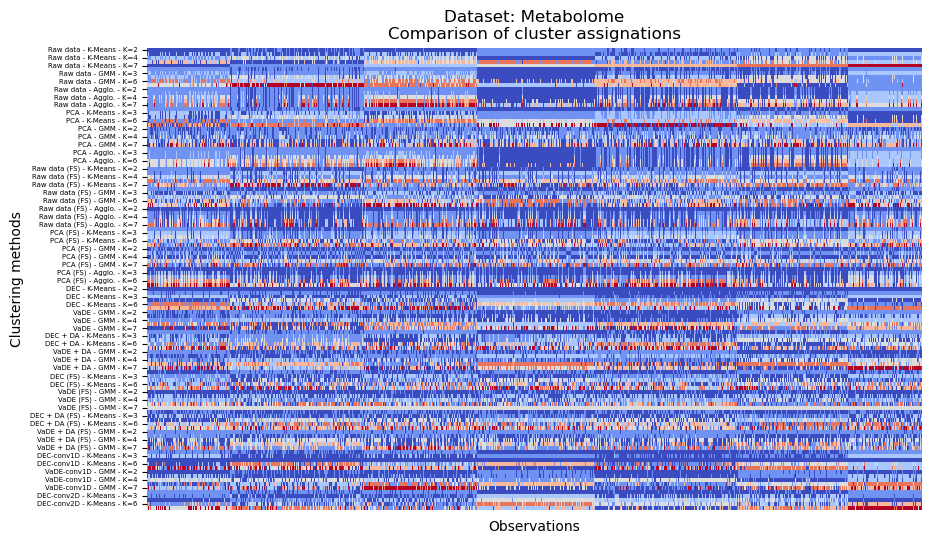
\includegraphics[width=\textwidth]{exposome_challenge/heatmap_clusters/metabol_uncorrected.png}
        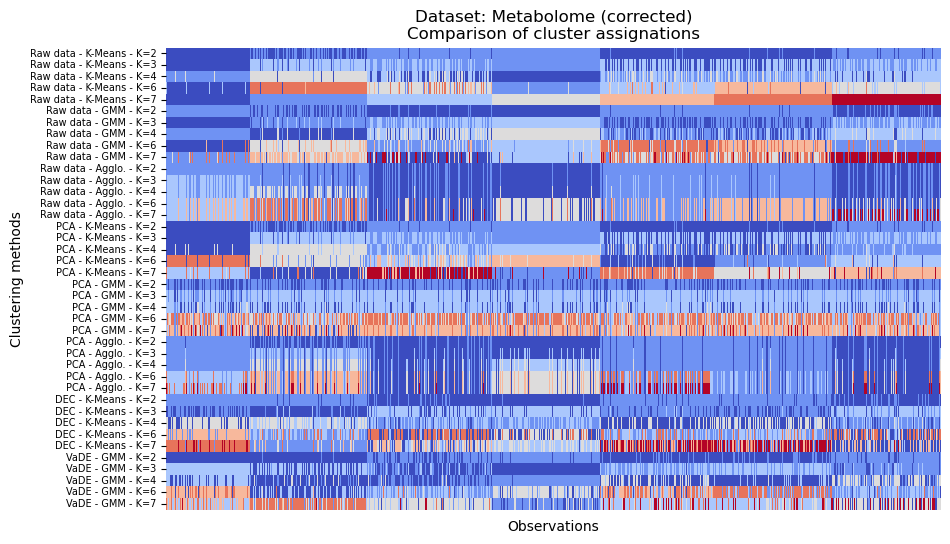
\includegraphics[width=\textwidth]{exposome_challenge/heatmap_clusters/metabol_corrected.png}
        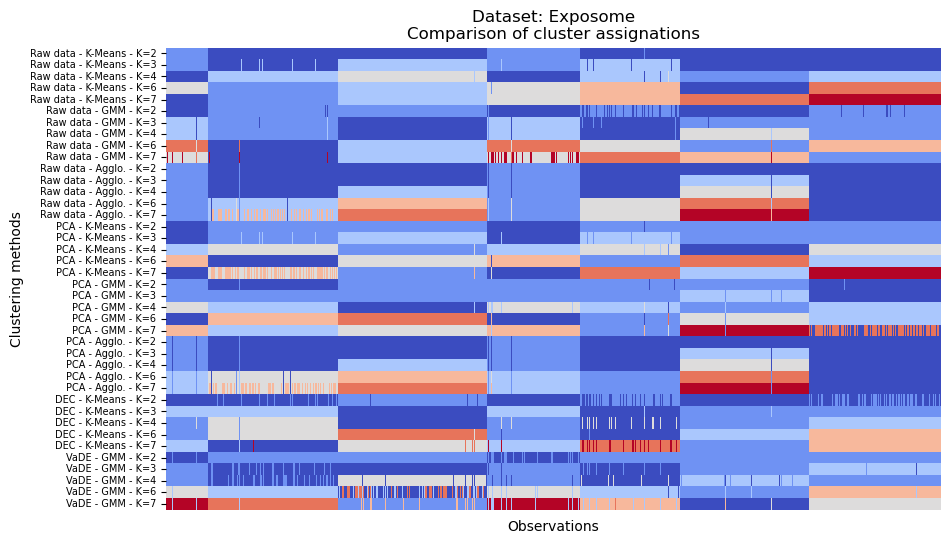
\includegraphics[width=\textwidth]{exposome_challenge/heatmap_clusters/exposome_uncorrected.png}
        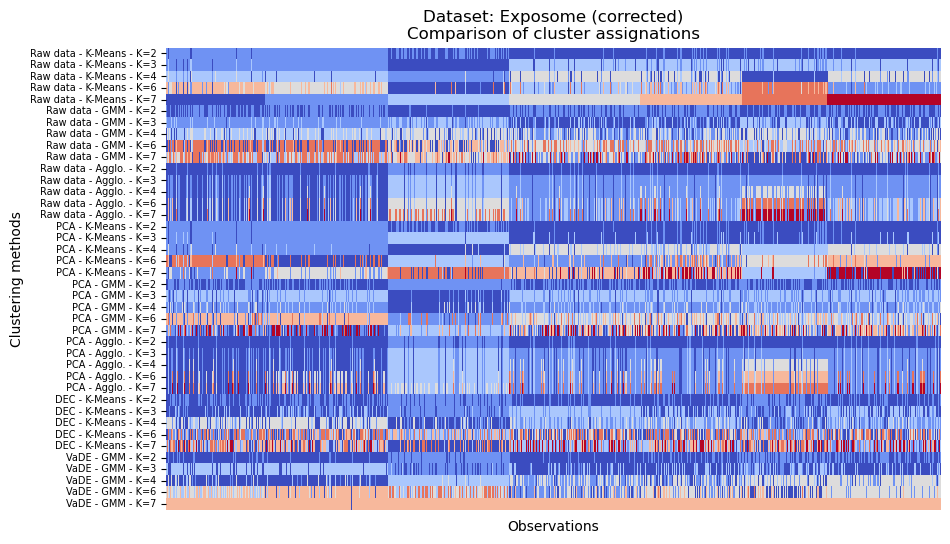
\includegraphics[width=\textwidth]{exposome_challenge/heatmap_clusters/exposome_corrected.png}
    \end{center}

    \clearpage

    \section{Gràfiques radials}

        A continuació es mostren les gràfiques radials
        que representen la distribució multivariant
        de les dades del fenotip i covariables,
        en segons dels clústers trobats.
        S'han ordenat en funció del conjunt de dades
        sobre el que s'han aplicat els mètodes de \textit{clustering}.

        \subsection{Conjunt de dades: metaboloma}

            \paragraph{Dades fenotip:} distribució multivariant en funció dels clústers.

            \begin{center}
                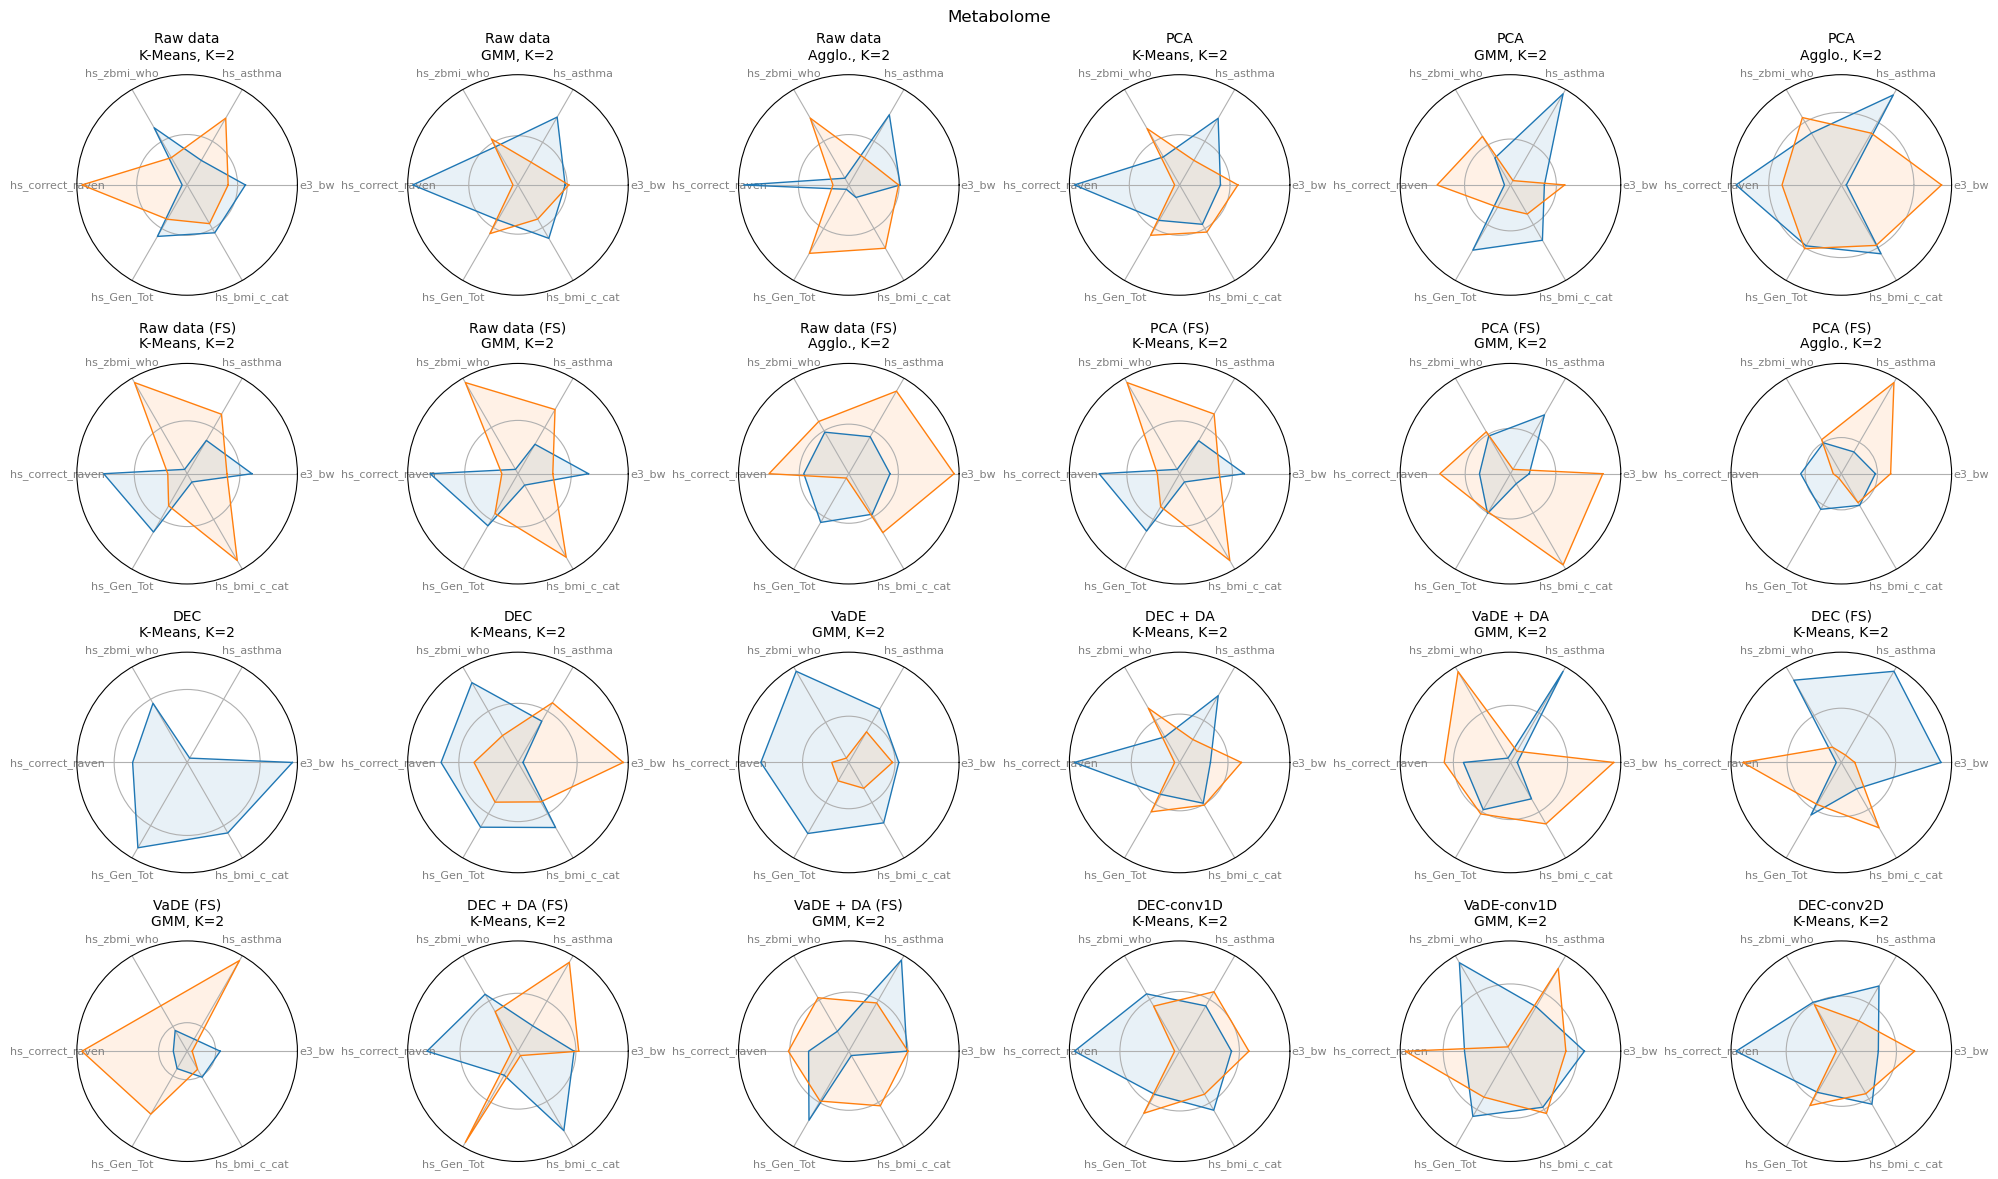
\includegraphics[width=\textwidth]{exposome_challenge/radialplots/metab_uncorr_feno_k2.png}
                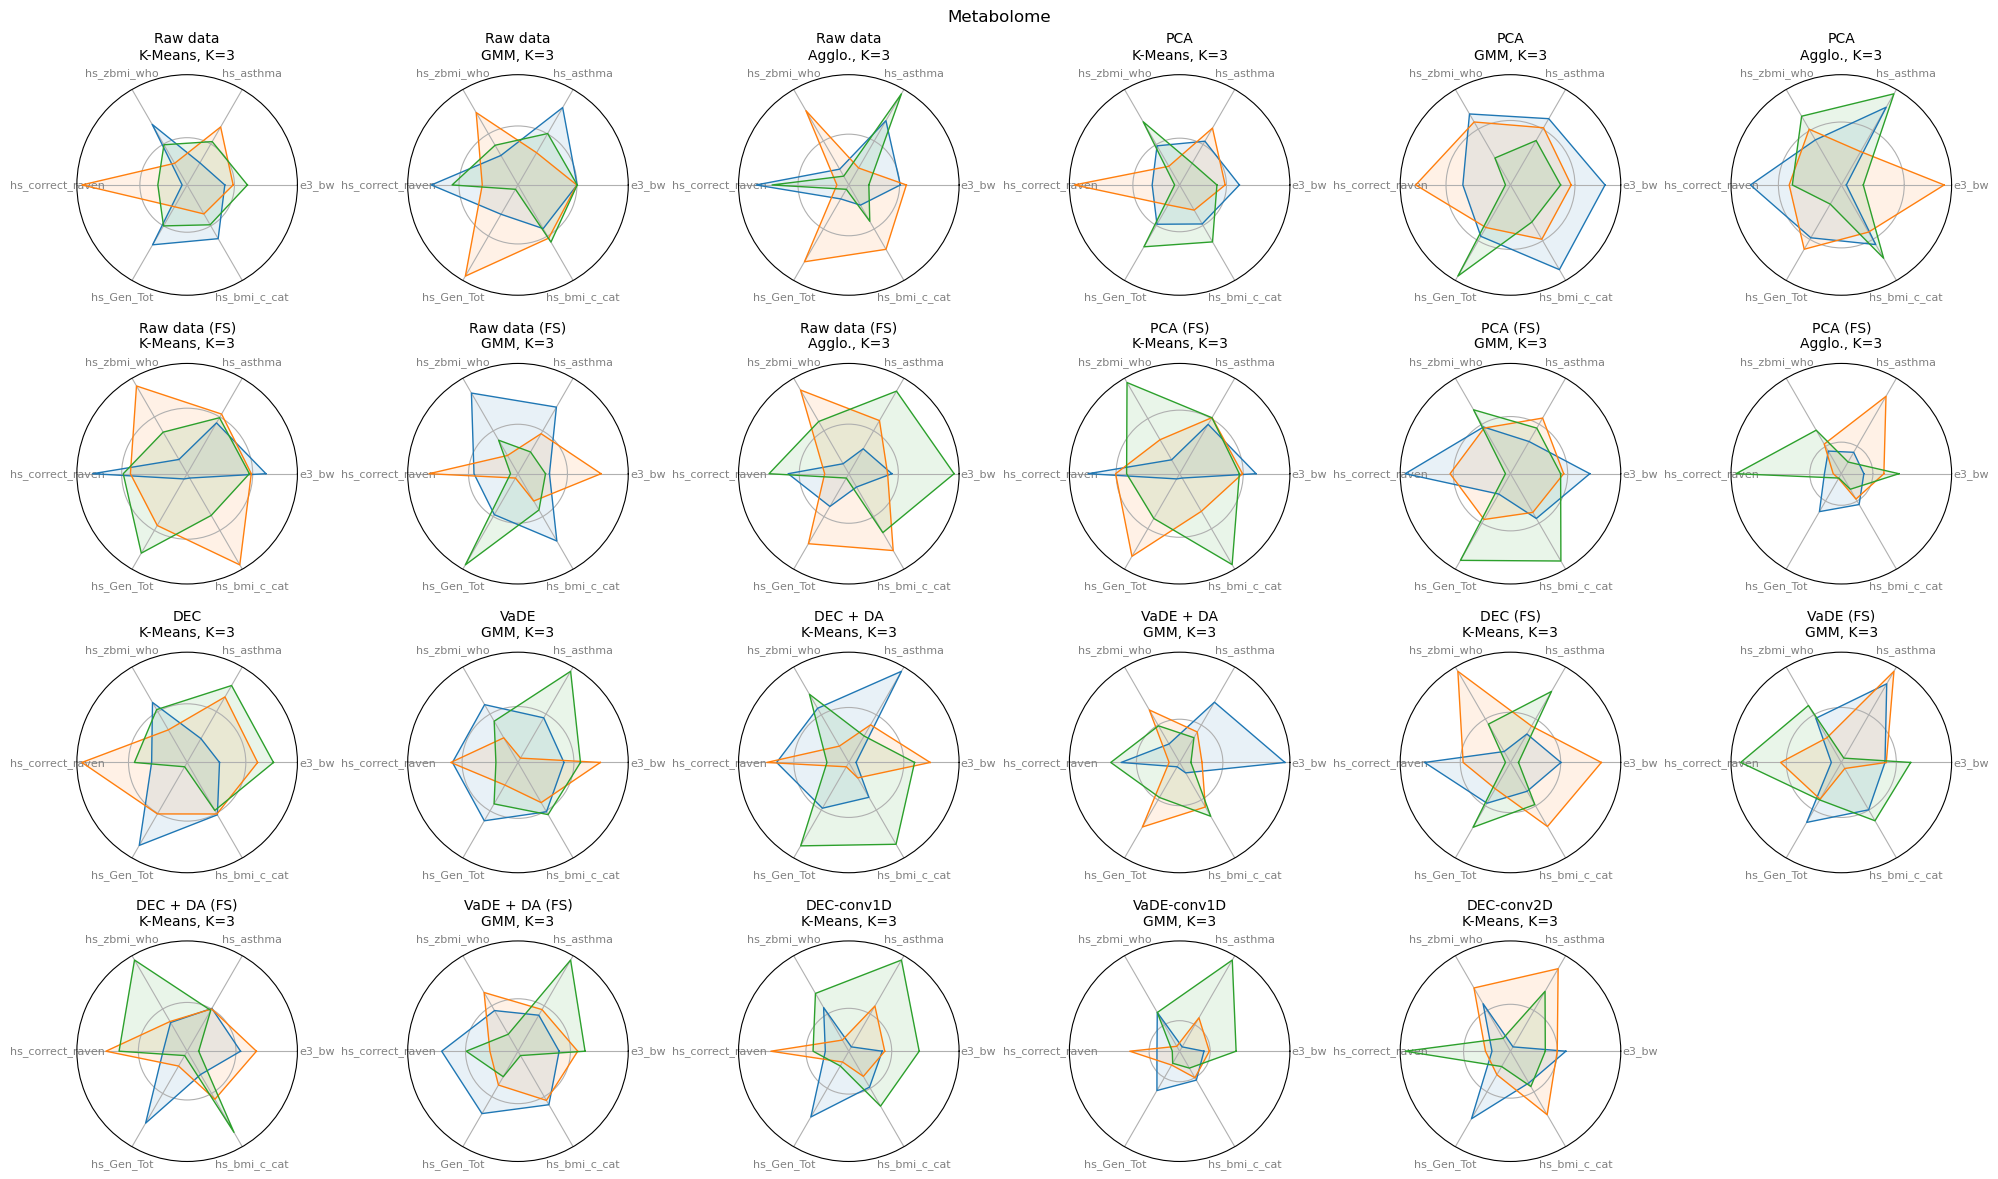
\includegraphics[width=\textwidth]{exposome_challenge/radialplots/metab_uncorr_feno_k3.png}
                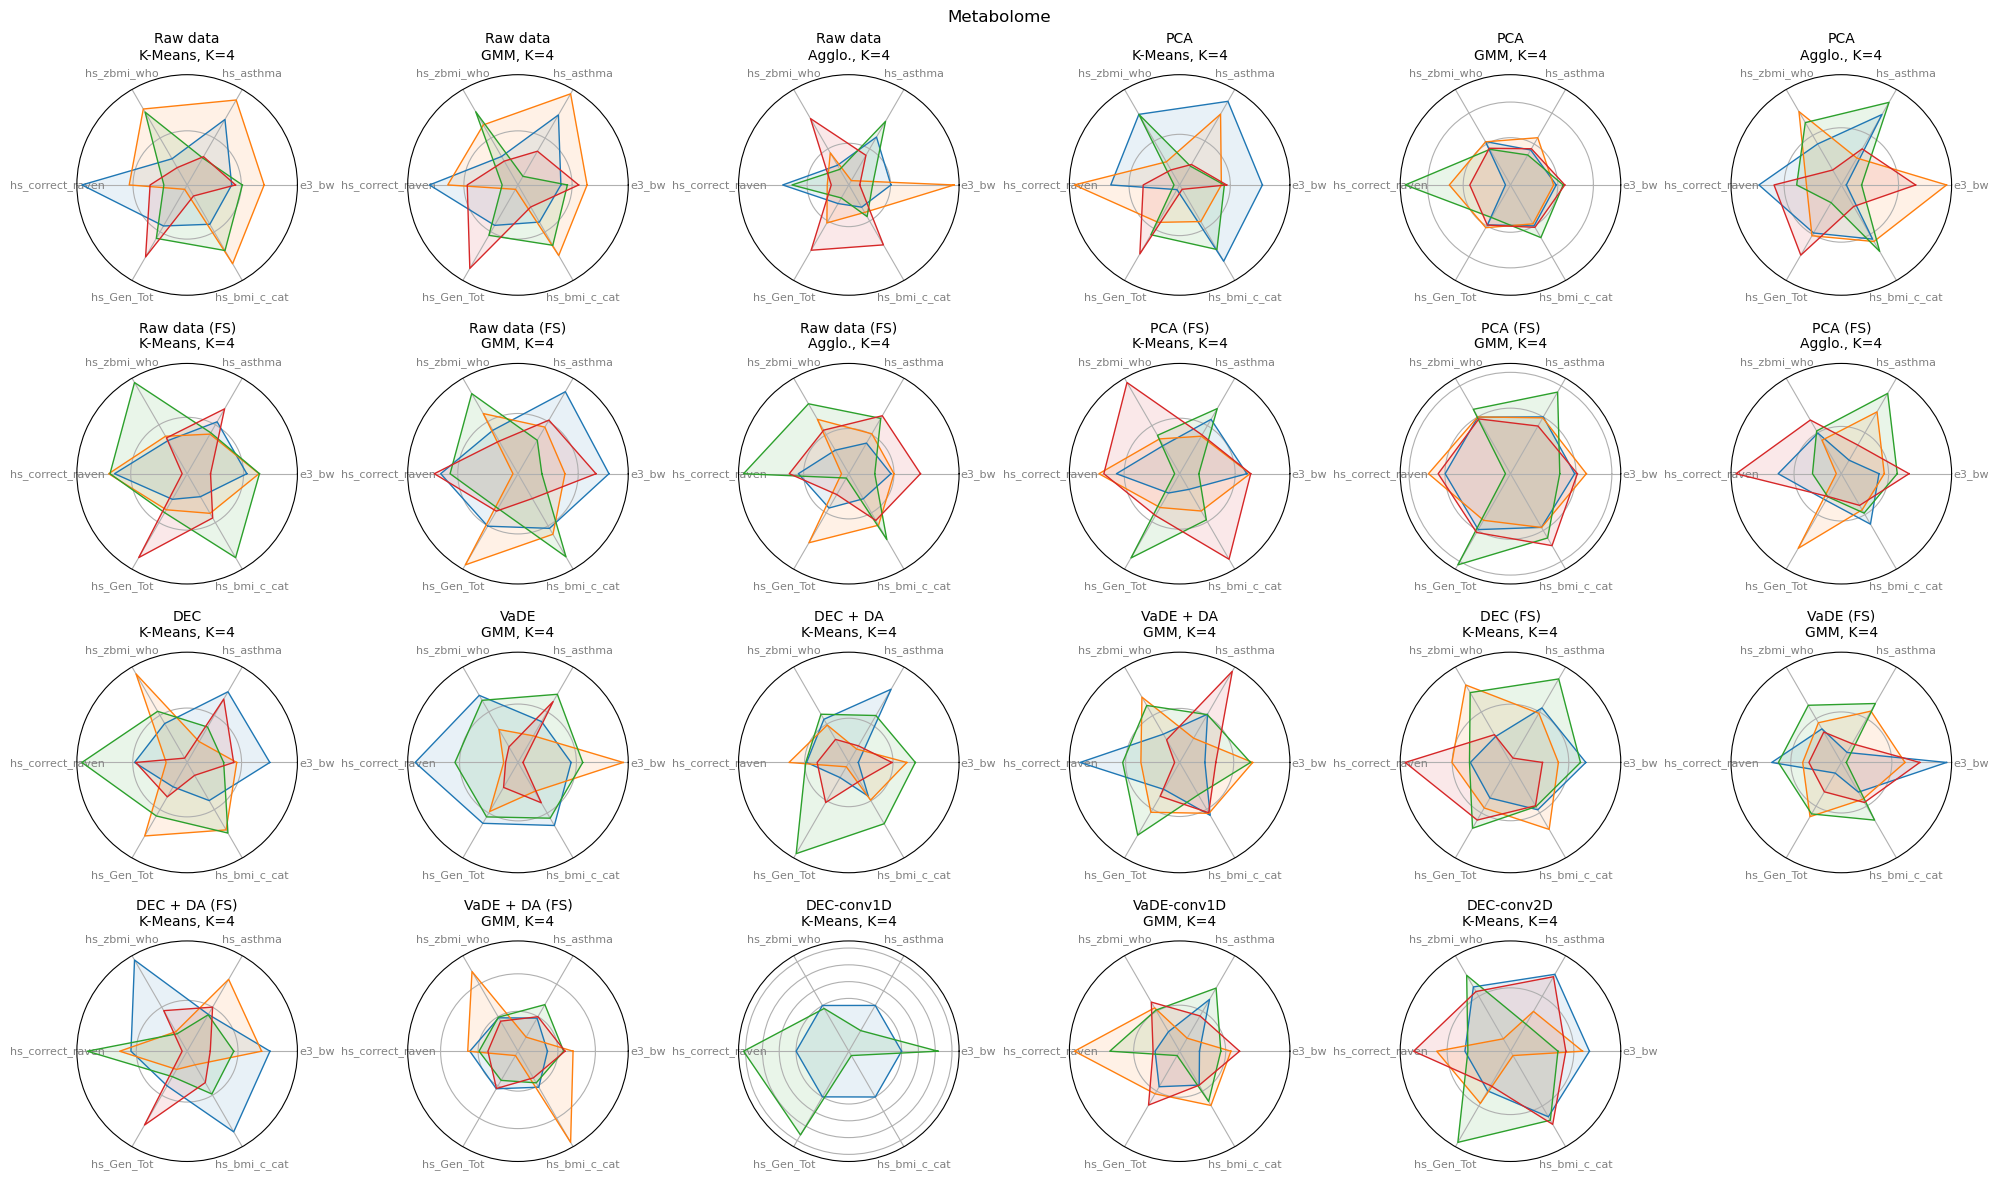
\includegraphics[width=\textwidth]{exposome_challenge/radialplots/metab_uncorr_feno_k4.png}
                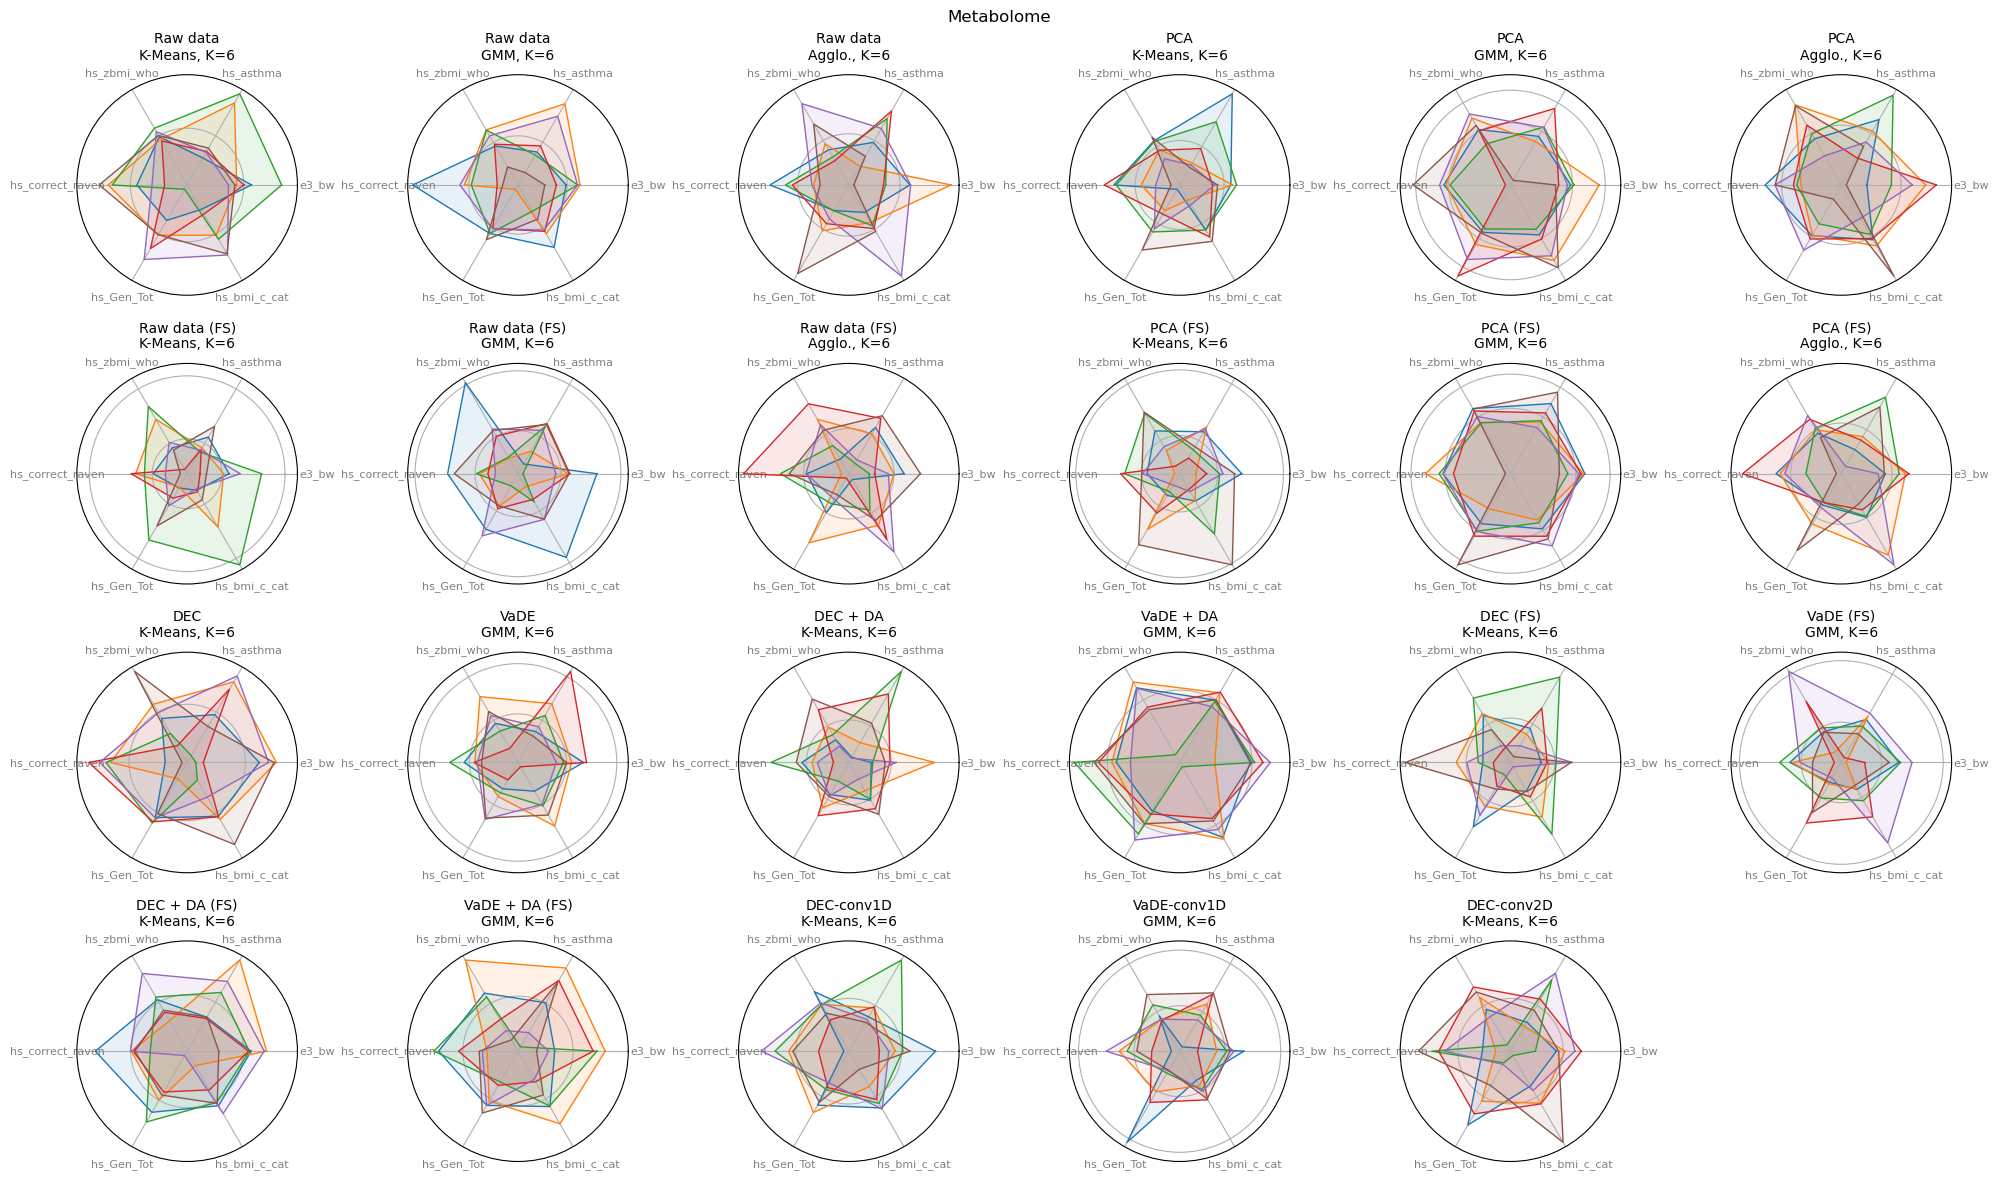
\includegraphics[width=\textwidth]{exposome_challenge/radialplots/metab_uncorr_feno_k6.png}
                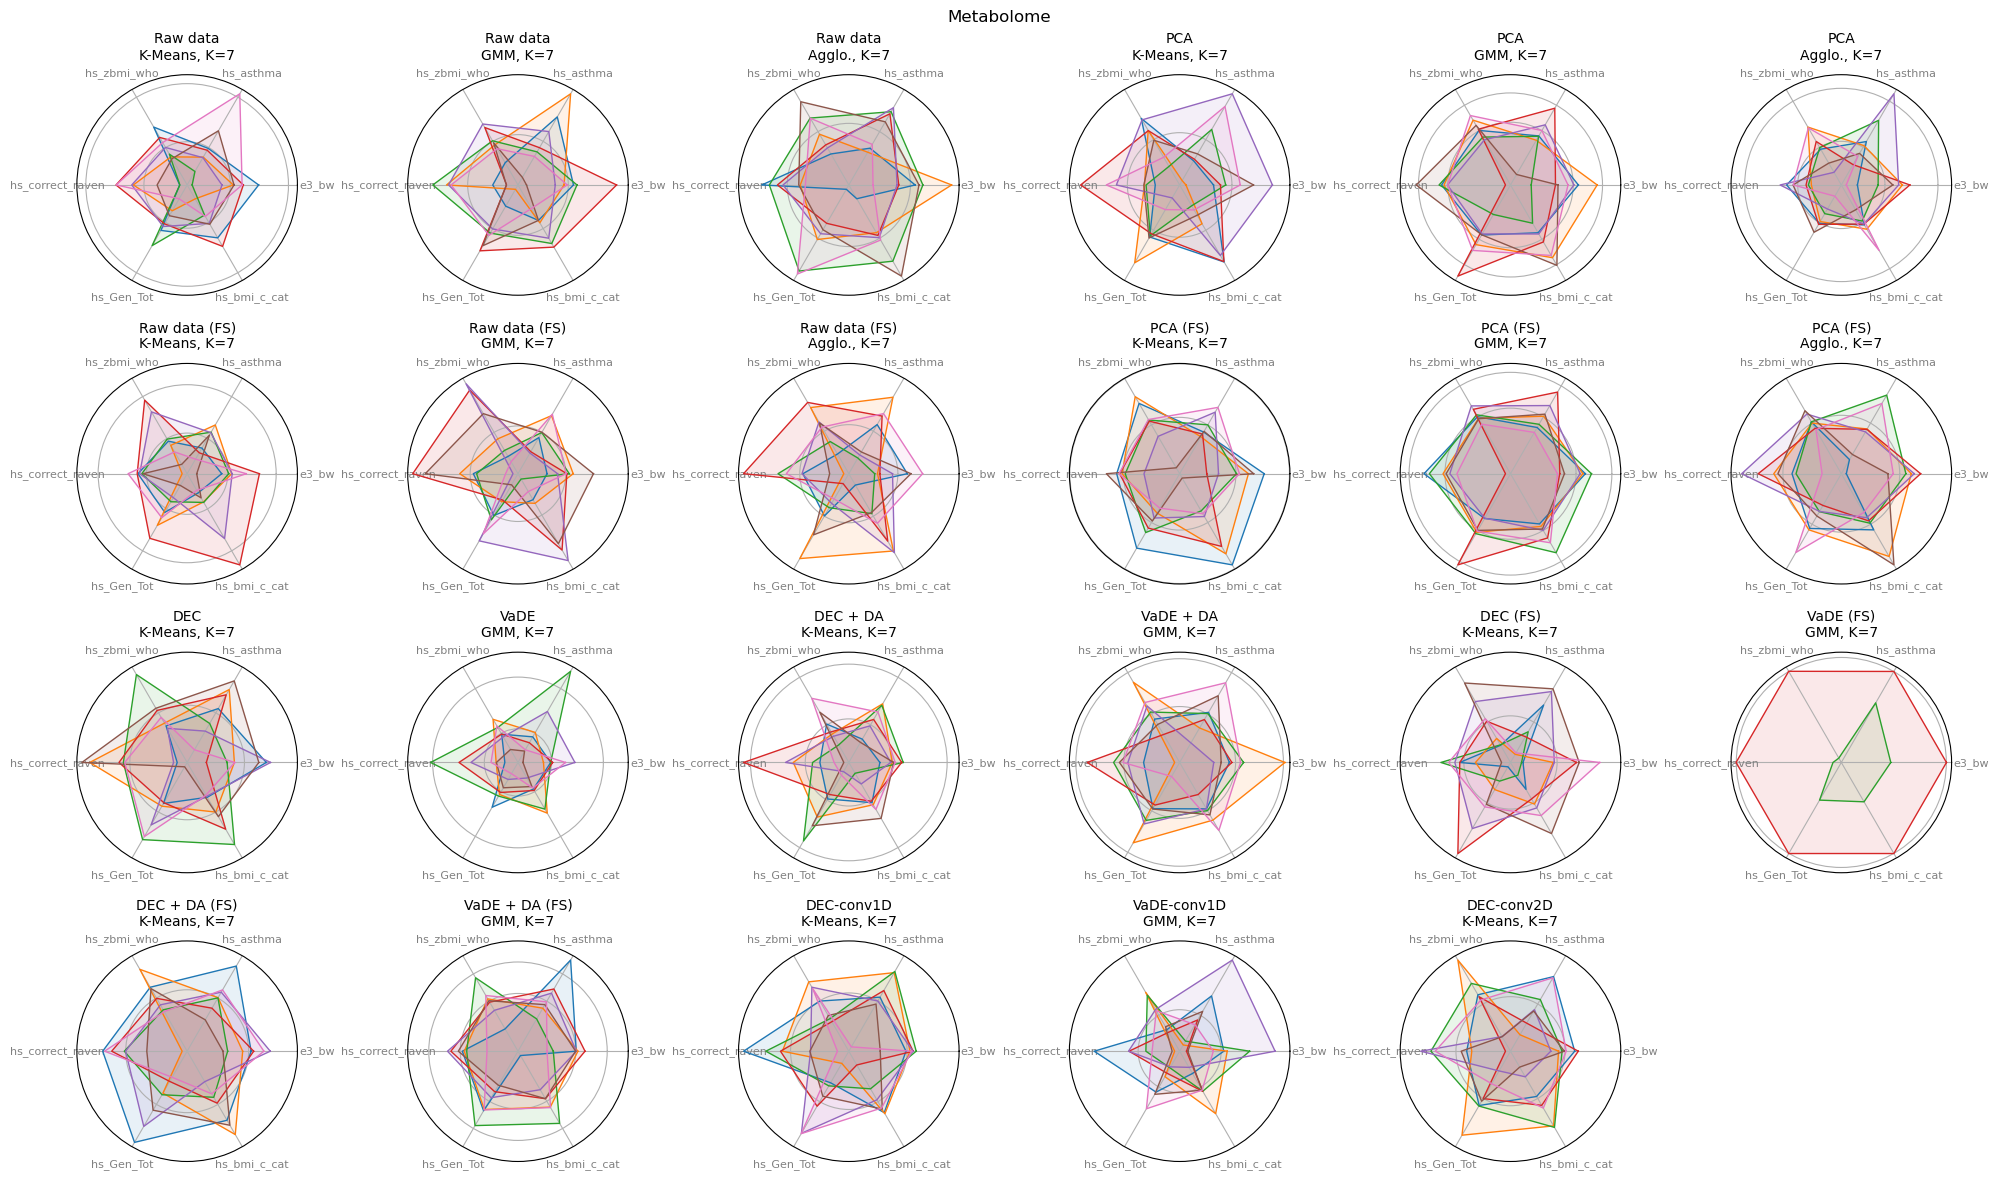
\includegraphics[width=\textwidth]{exposome_challenge/radialplots/metab_uncorr_feno_k7.png}
            \end{center}

            \paragraph{Dades covariables:} distribució multivariant en funció dels clústers.

            \begin{center}
                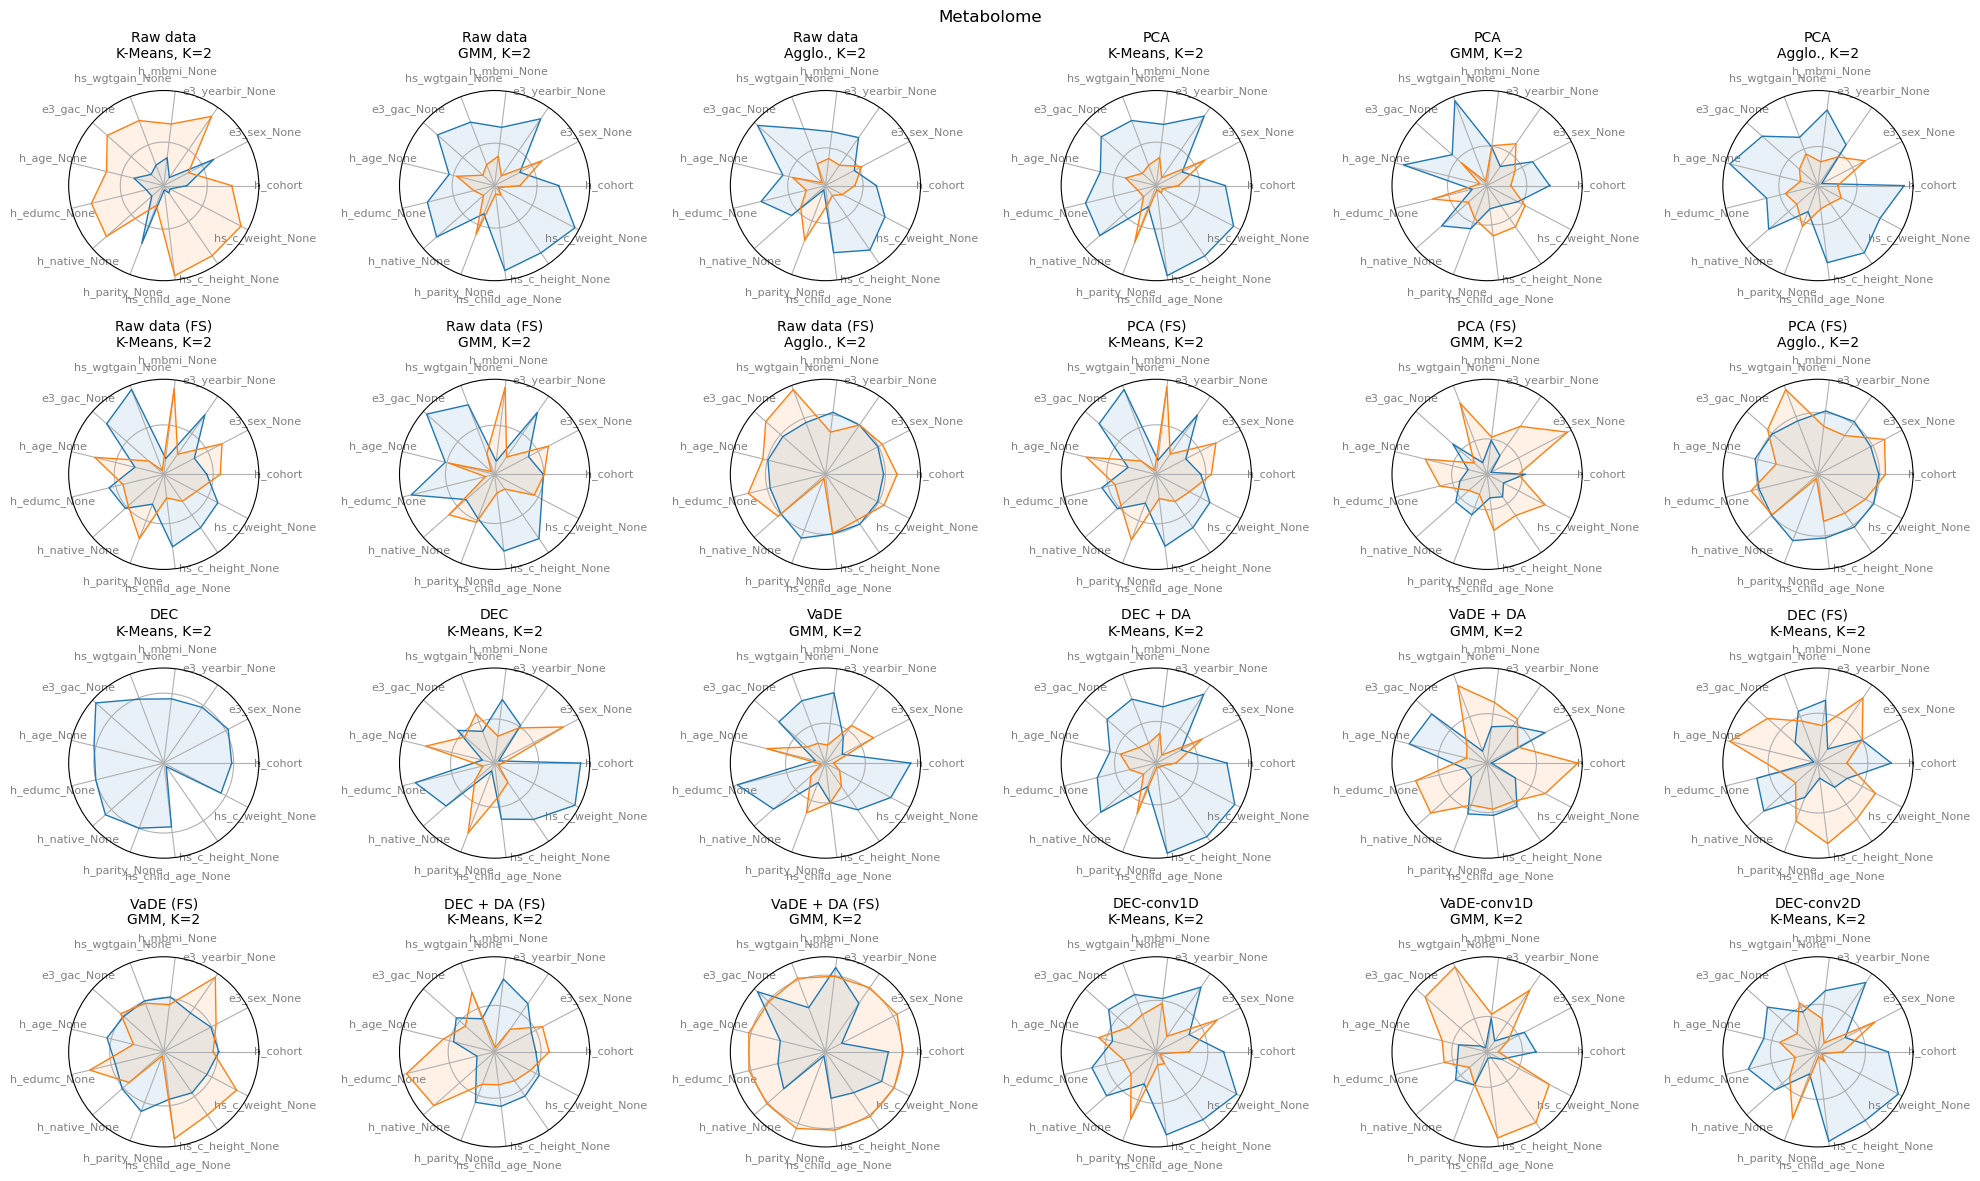
\includegraphics[width=\textwidth]{exposome_challenge/radialplots/metab_uncorr_covars_k2.png}
                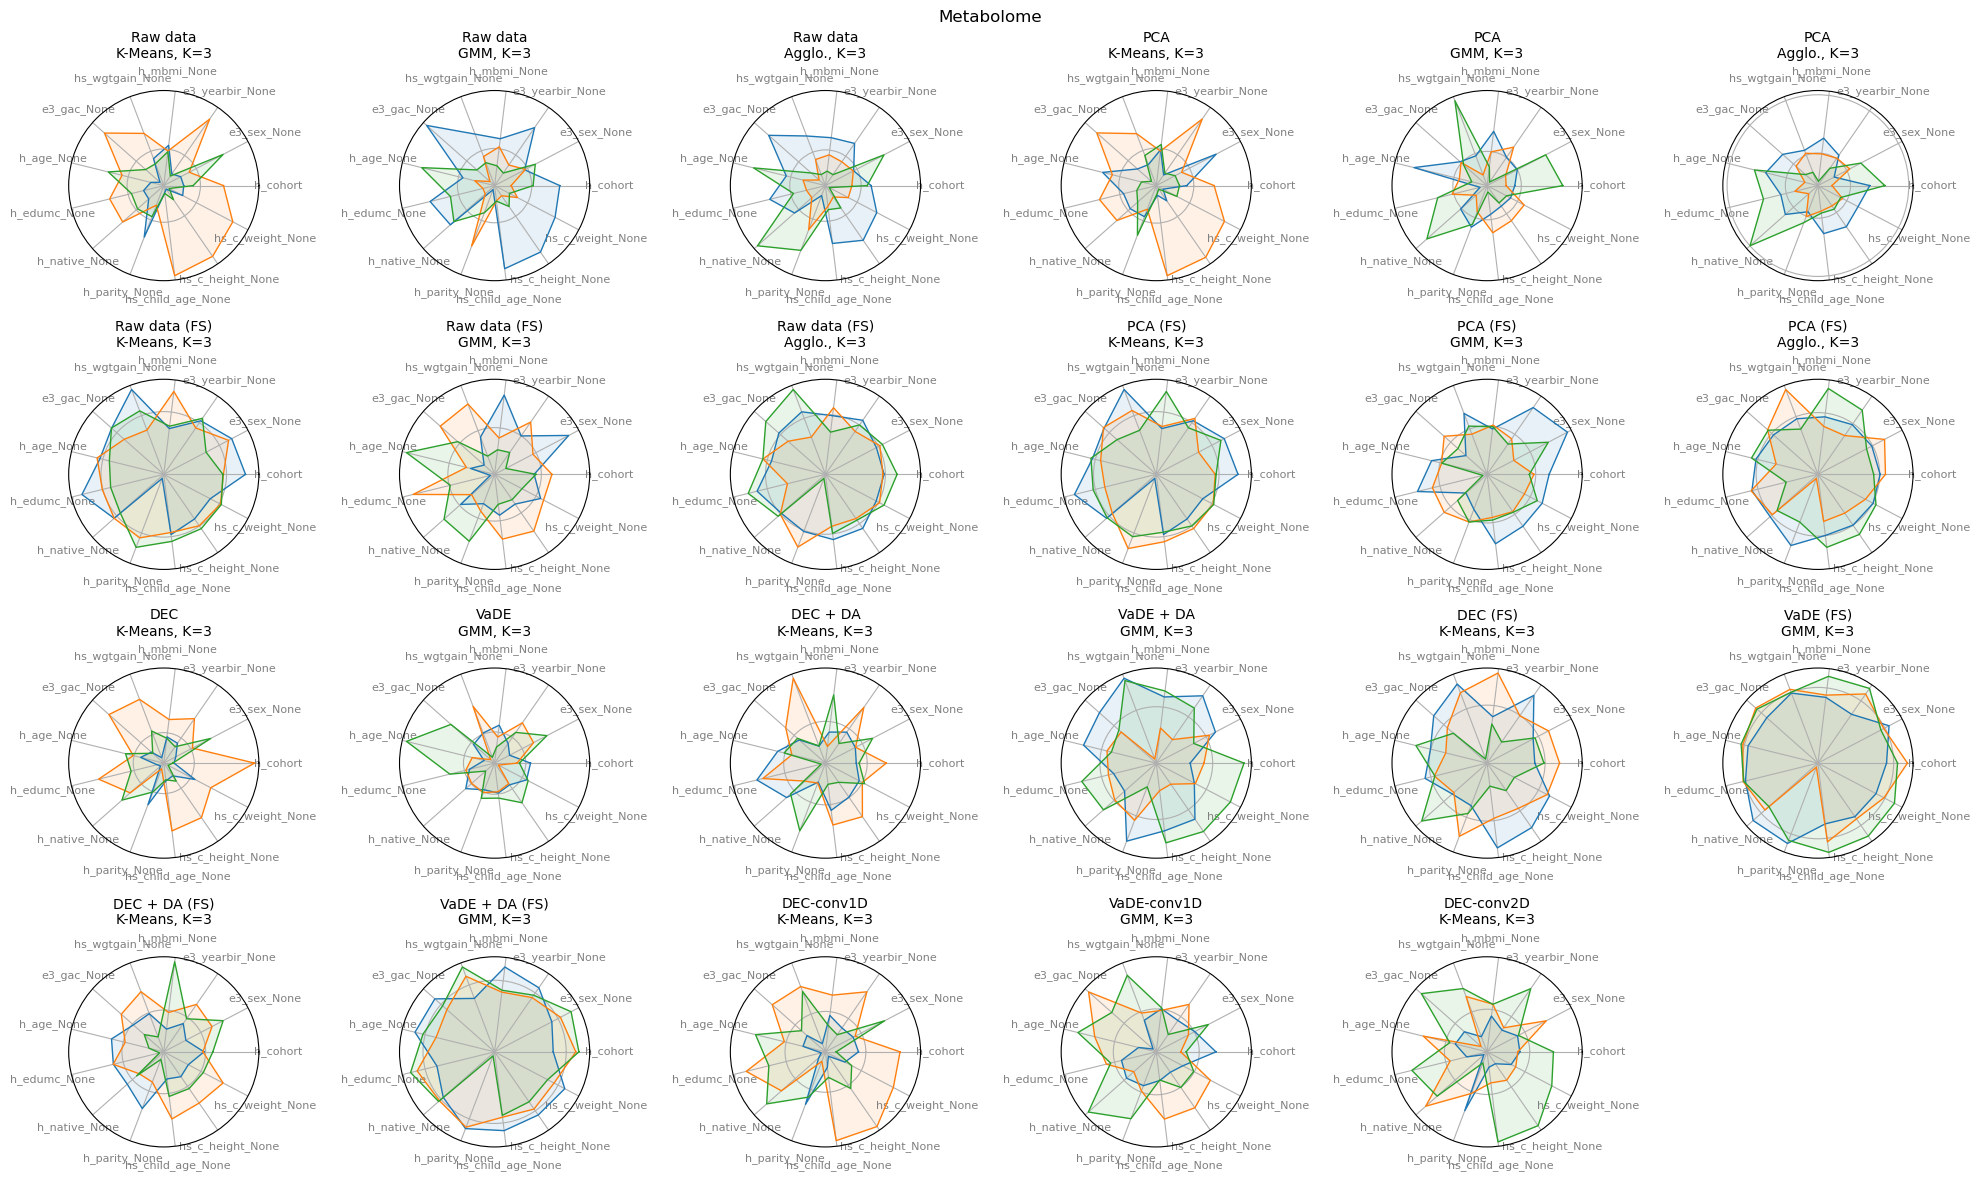
\includegraphics[width=\textwidth]{exposome_challenge/radialplots/metab_uncorr_covars_k3.png}
                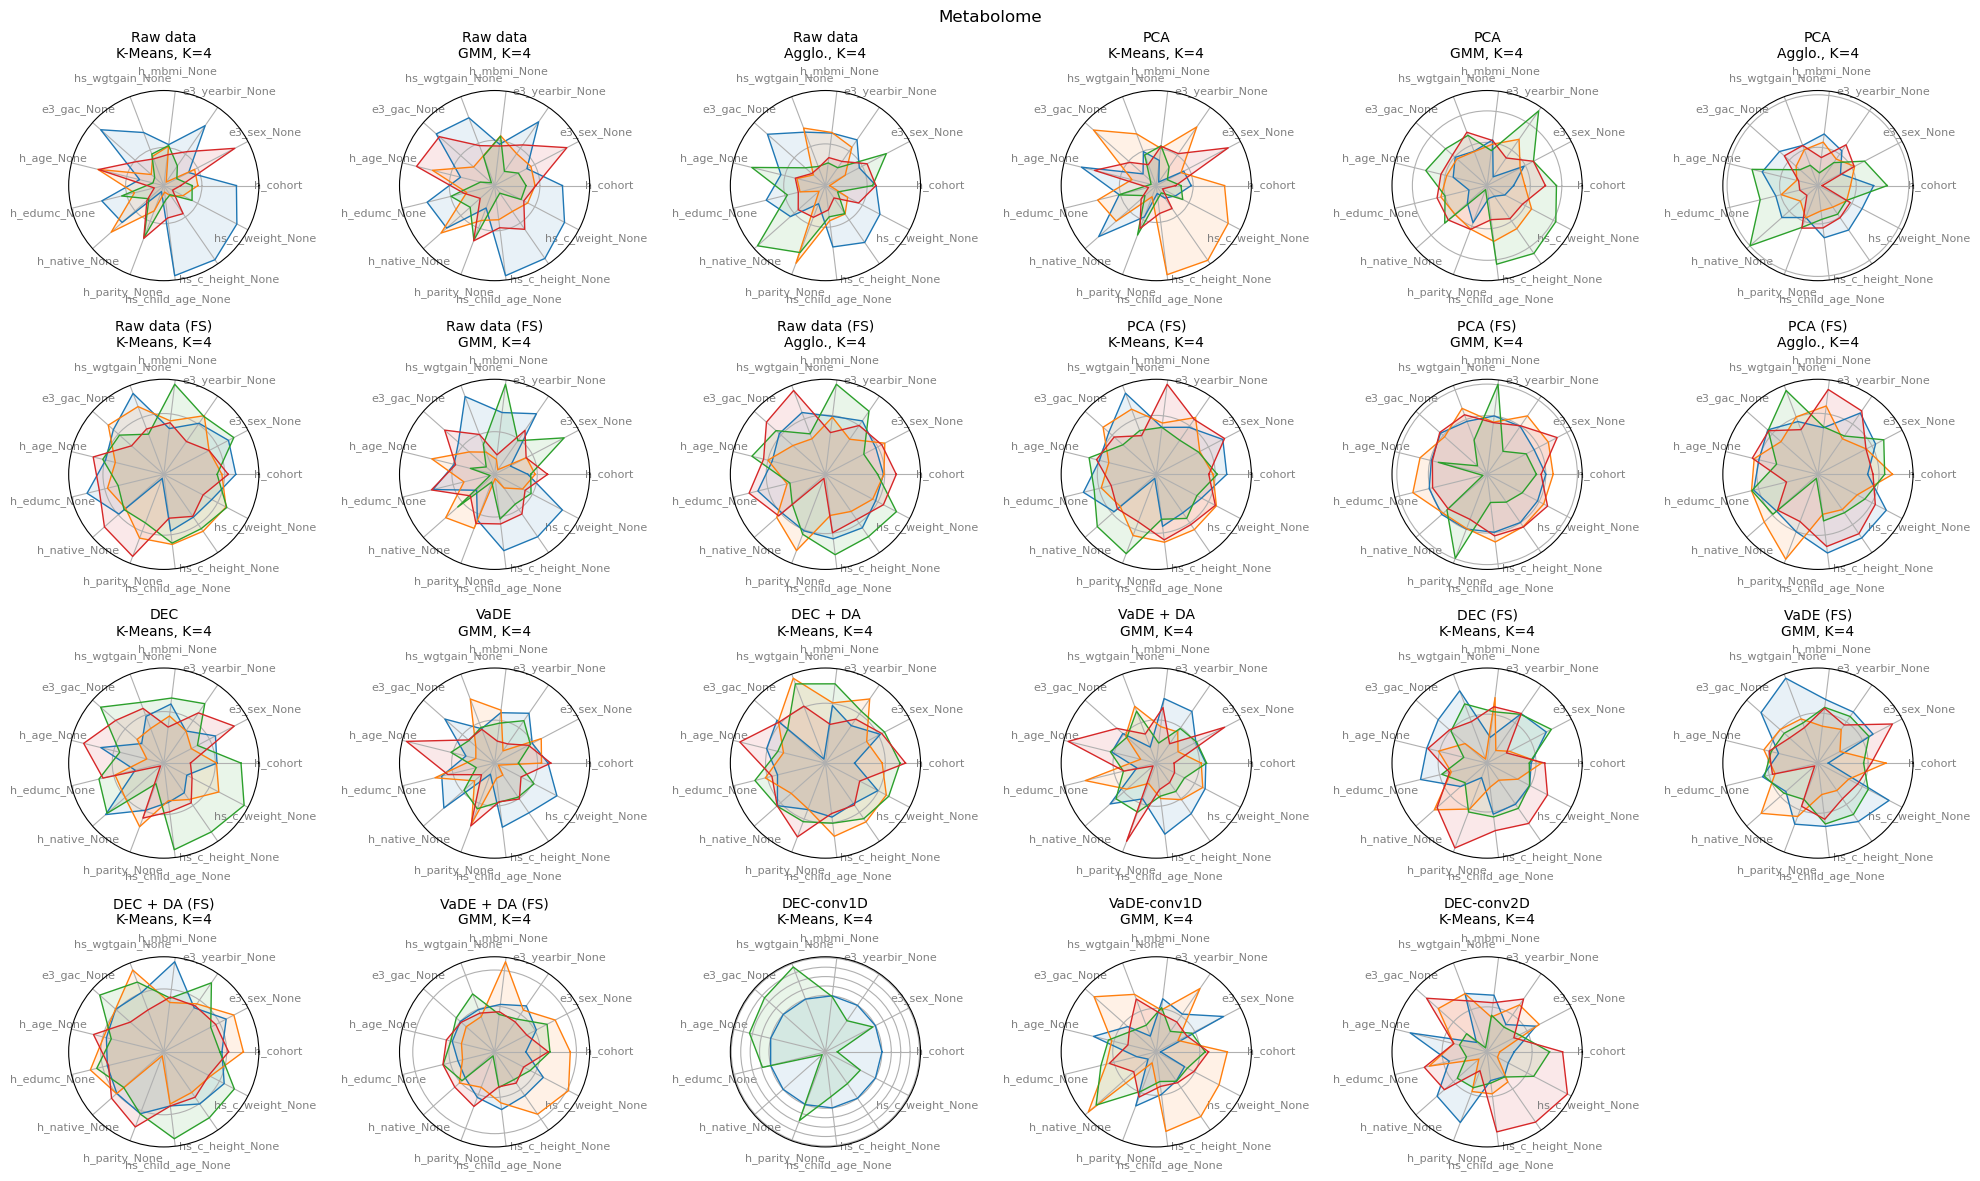
\includegraphics[width=\textwidth]{exposome_challenge/radialplots/metab_uncorr_covars_k4.png}
                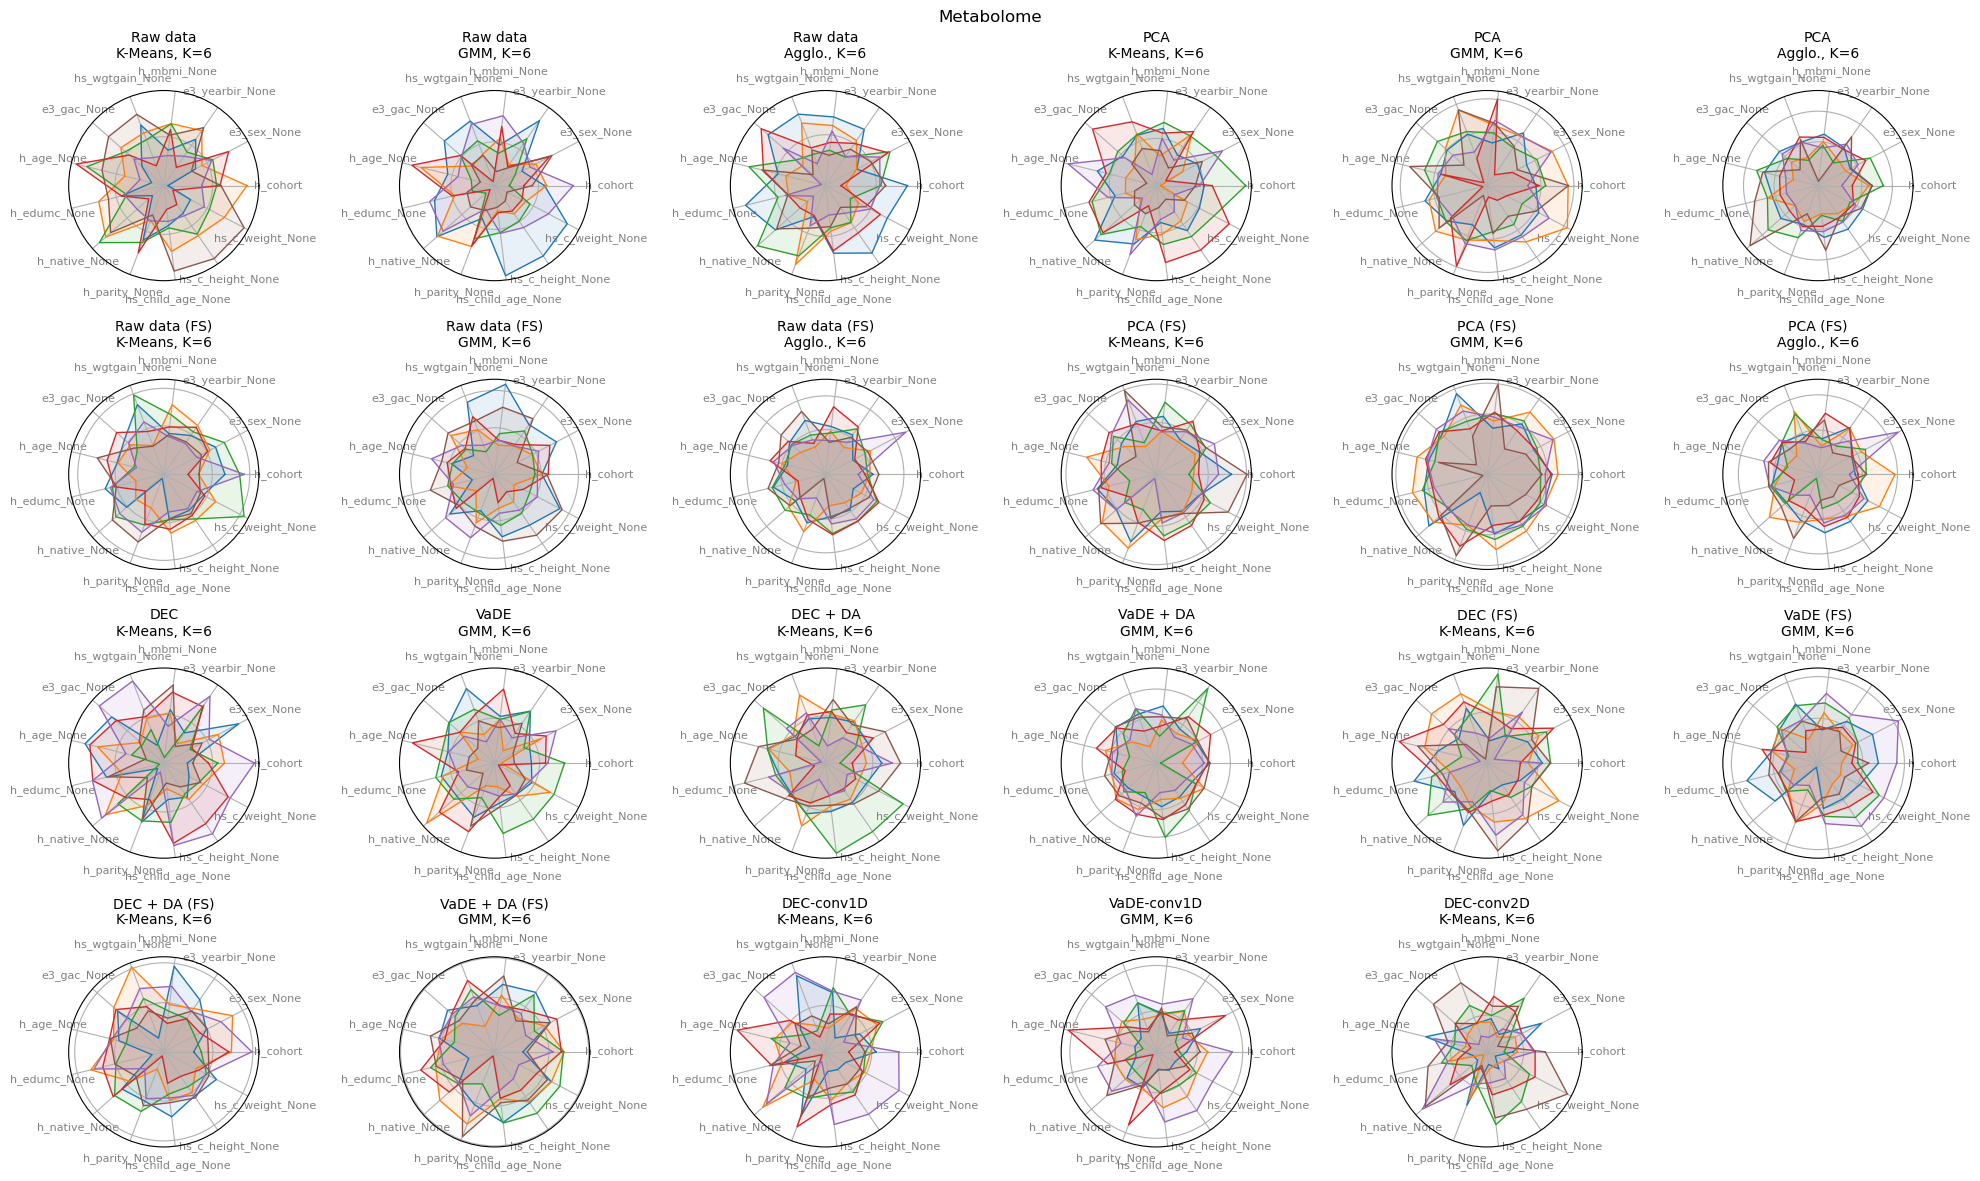
\includegraphics[width=\textwidth]{exposome_challenge/radialplots/metab_uncorr_covars_k6.png}
                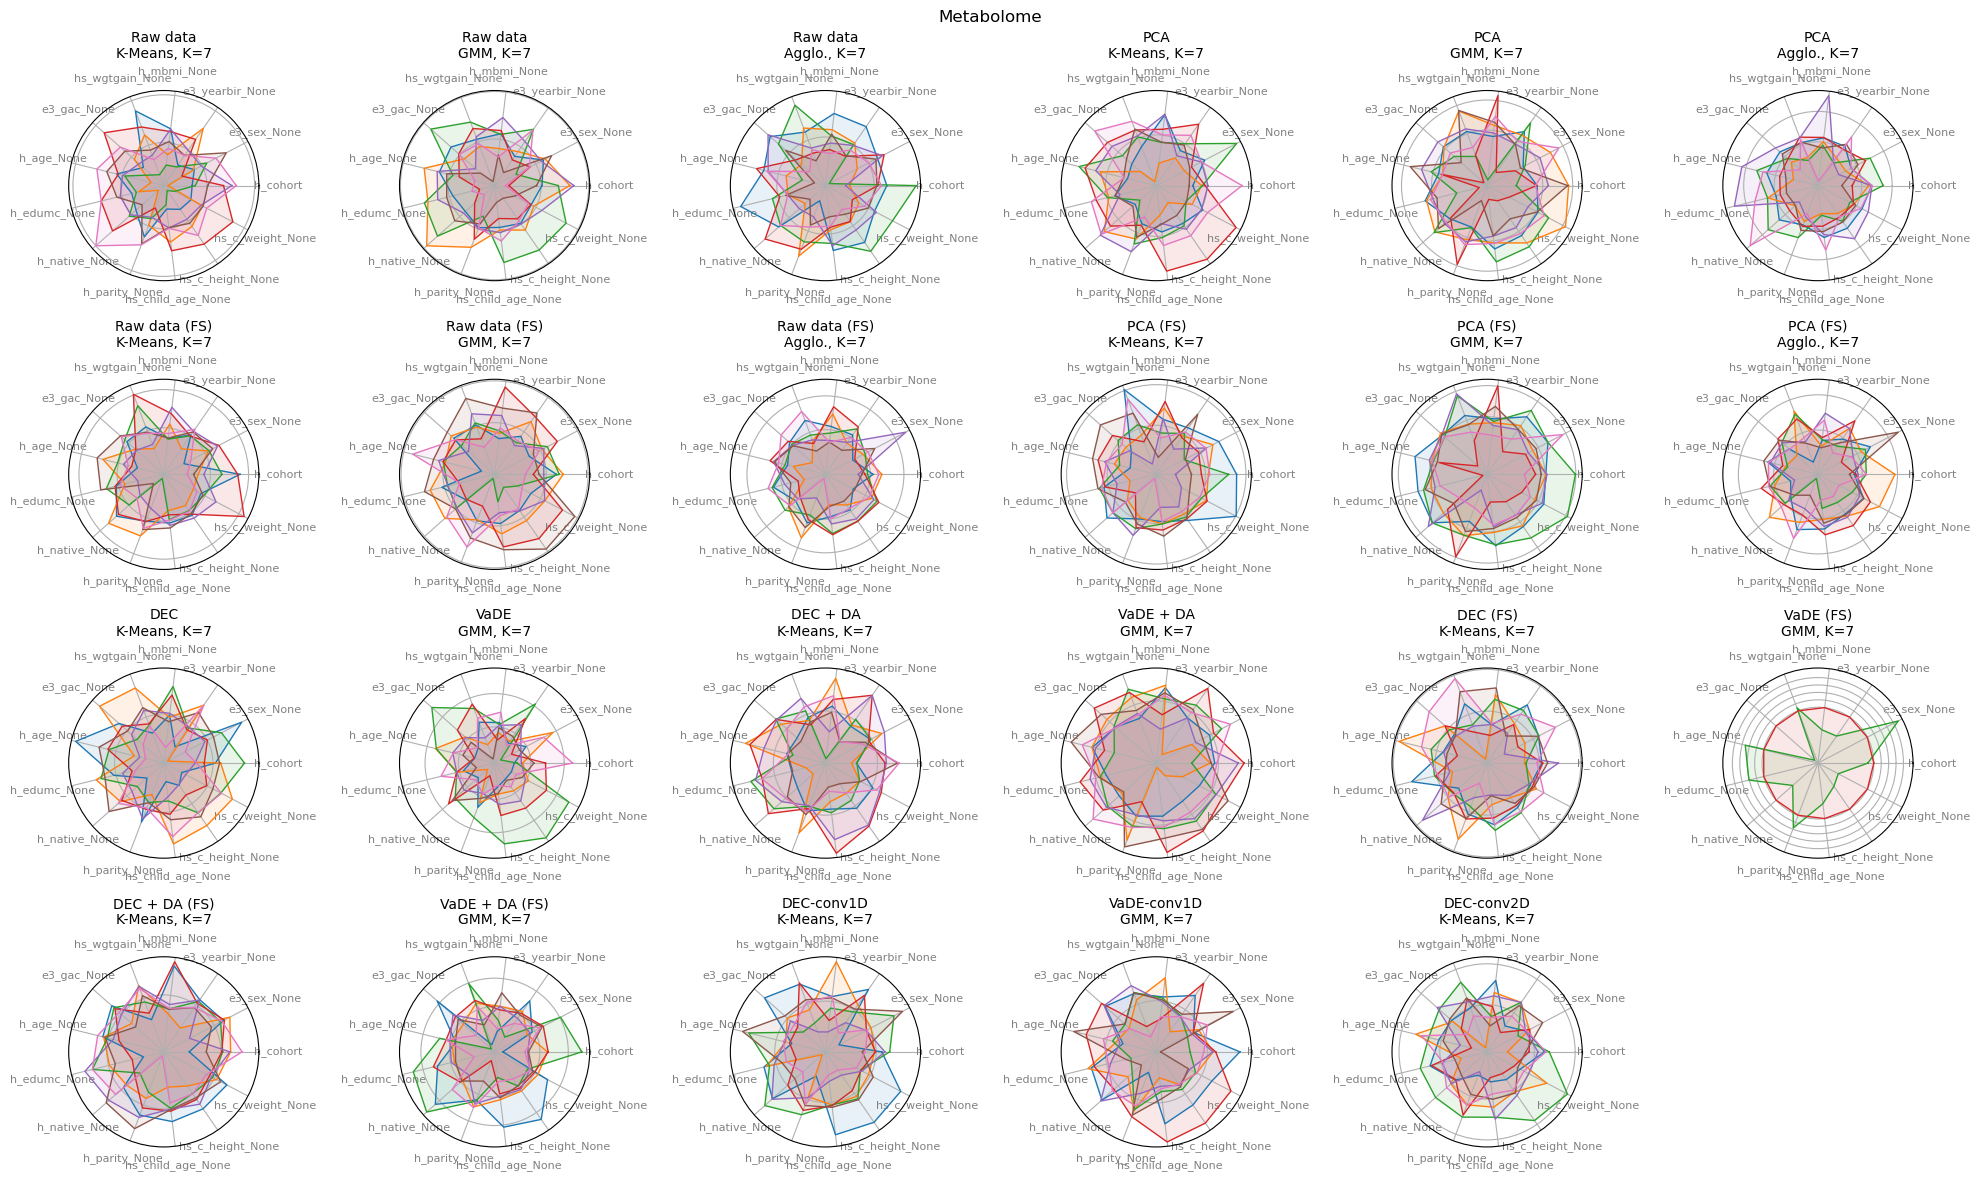
\includegraphics[width=\textwidth]{exposome_challenge/radialplots/metab_uncorr_covars_k7.png}
            \end{center}

            \paragraph{Dades metaboloma:} distribució multivariant en funció dels clústers (20 variables amb major variablitat).

            \begin{center}
                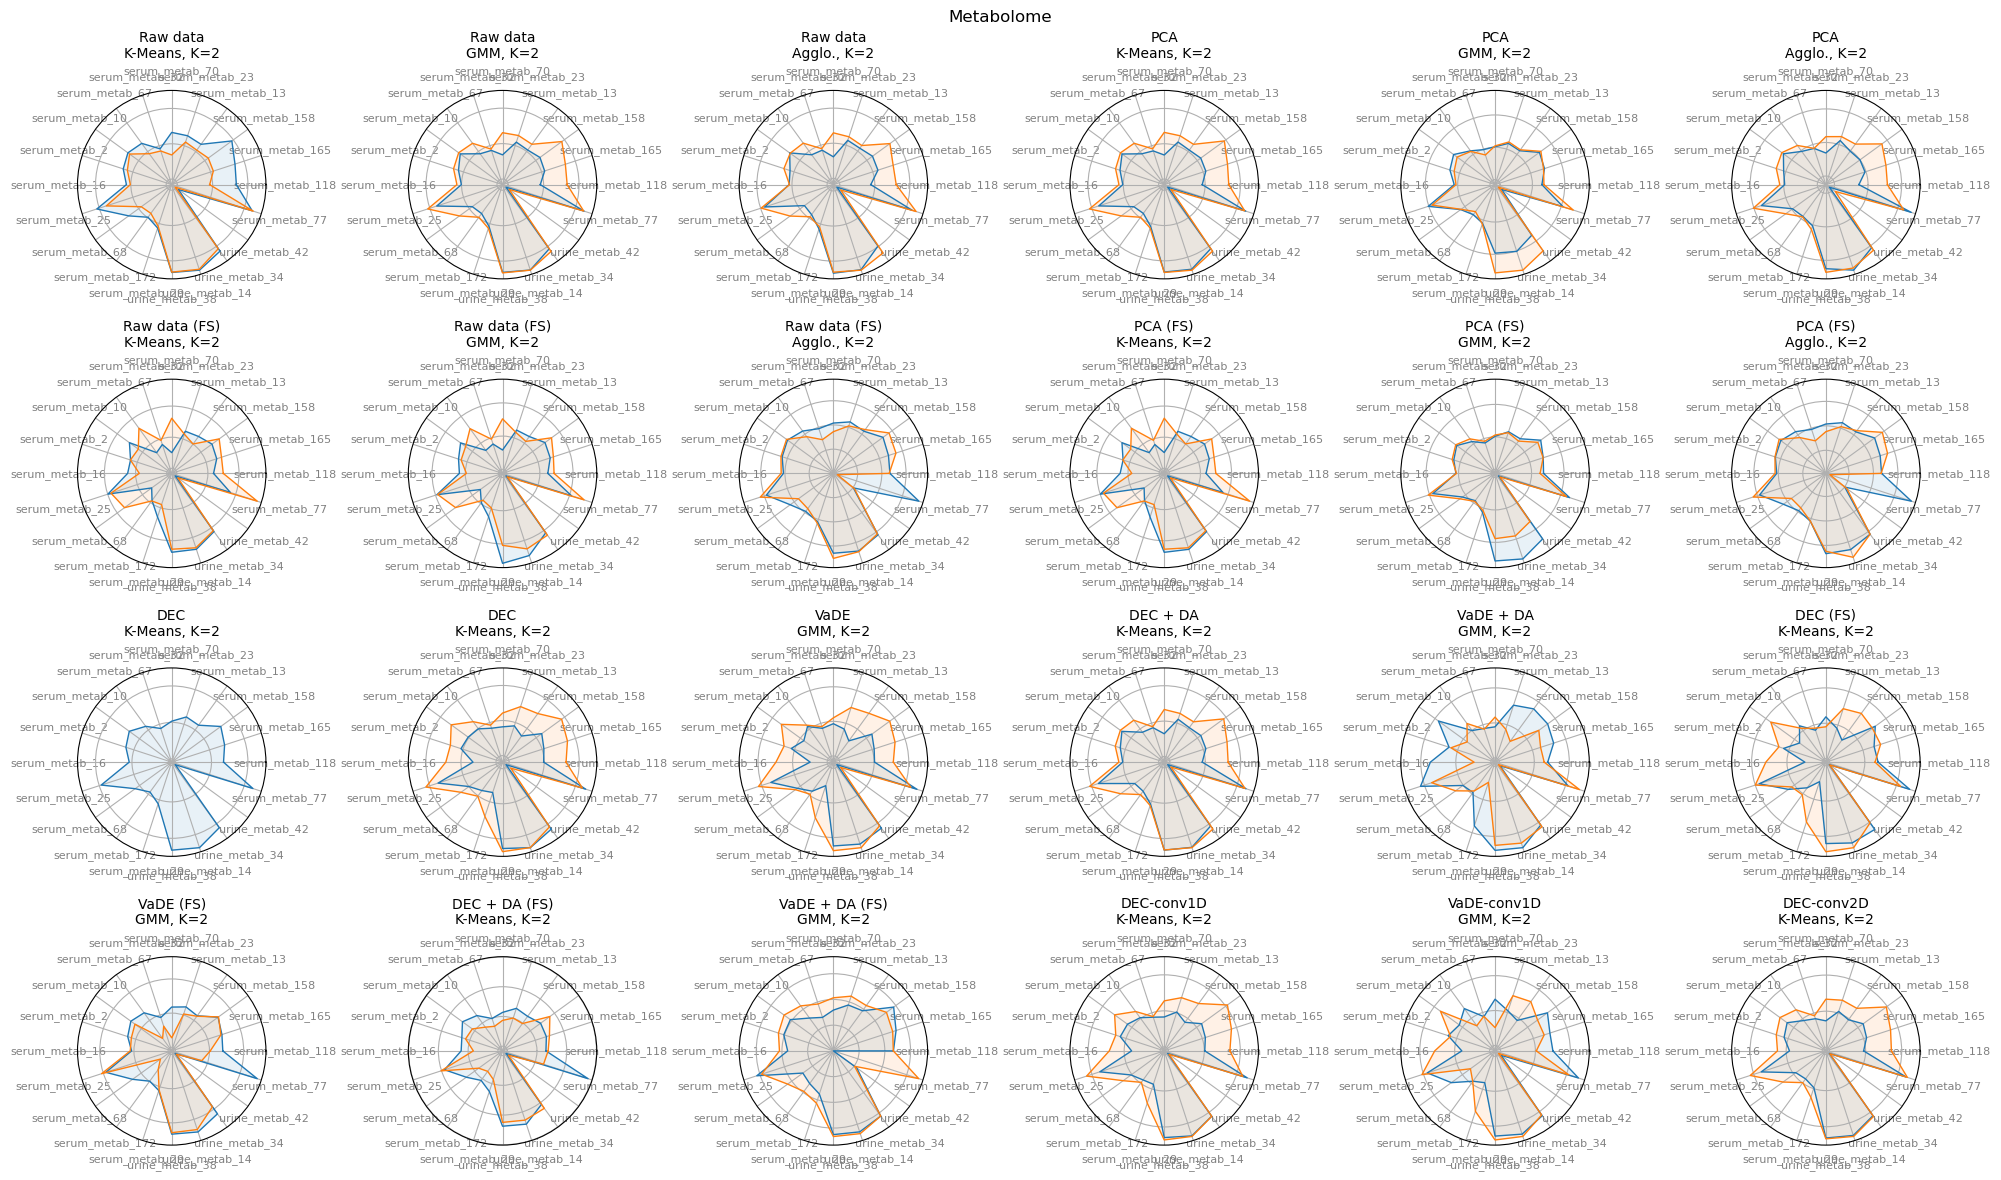
\includegraphics[width=\textwidth]{exposome_challenge/radialplots/metab_uncorr_mostvarfeat_k2.png}
                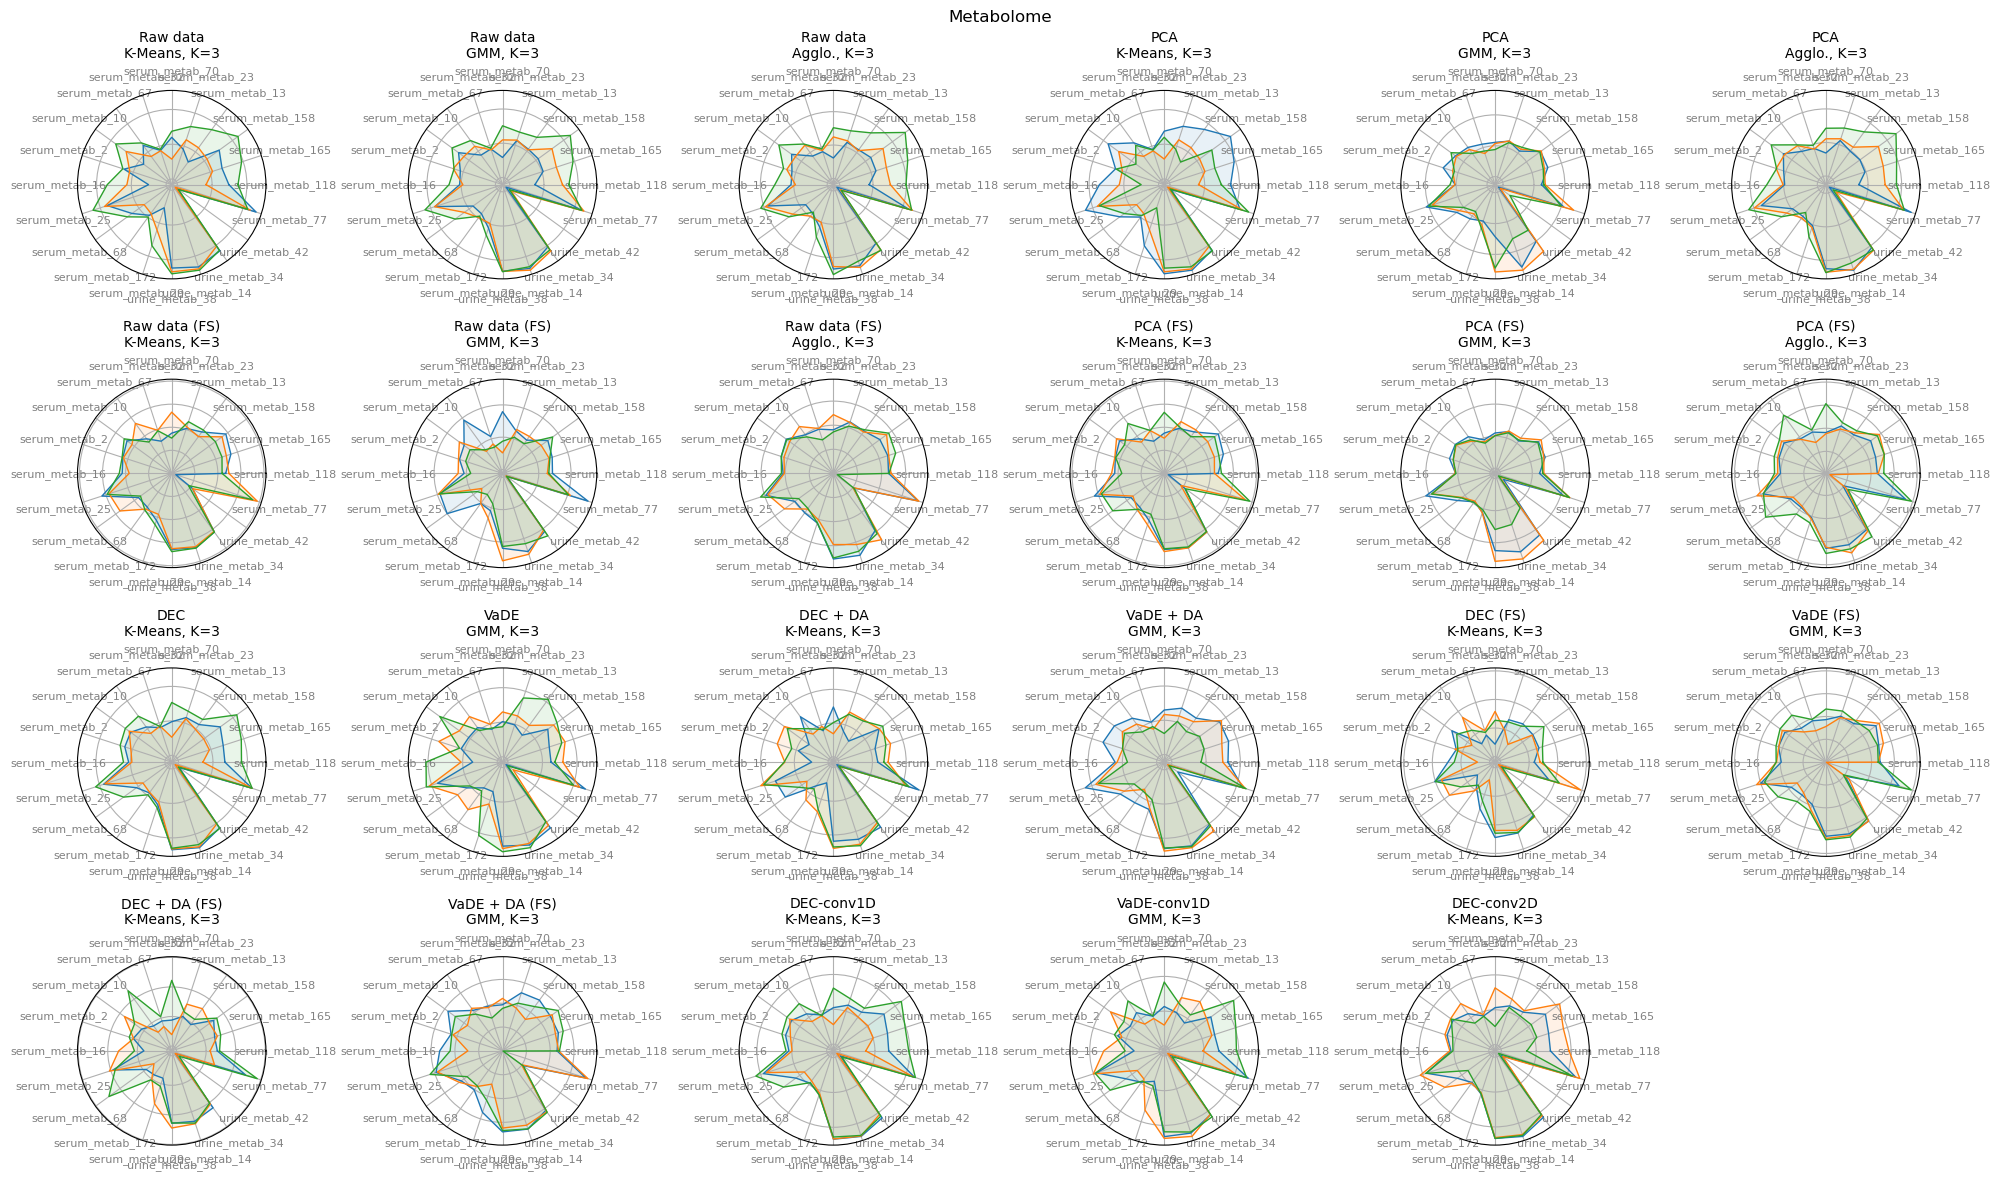
\includegraphics[width=\textwidth]{exposome_challenge/radialplots/metab_uncorr_mostvarfeat_k3.png}
                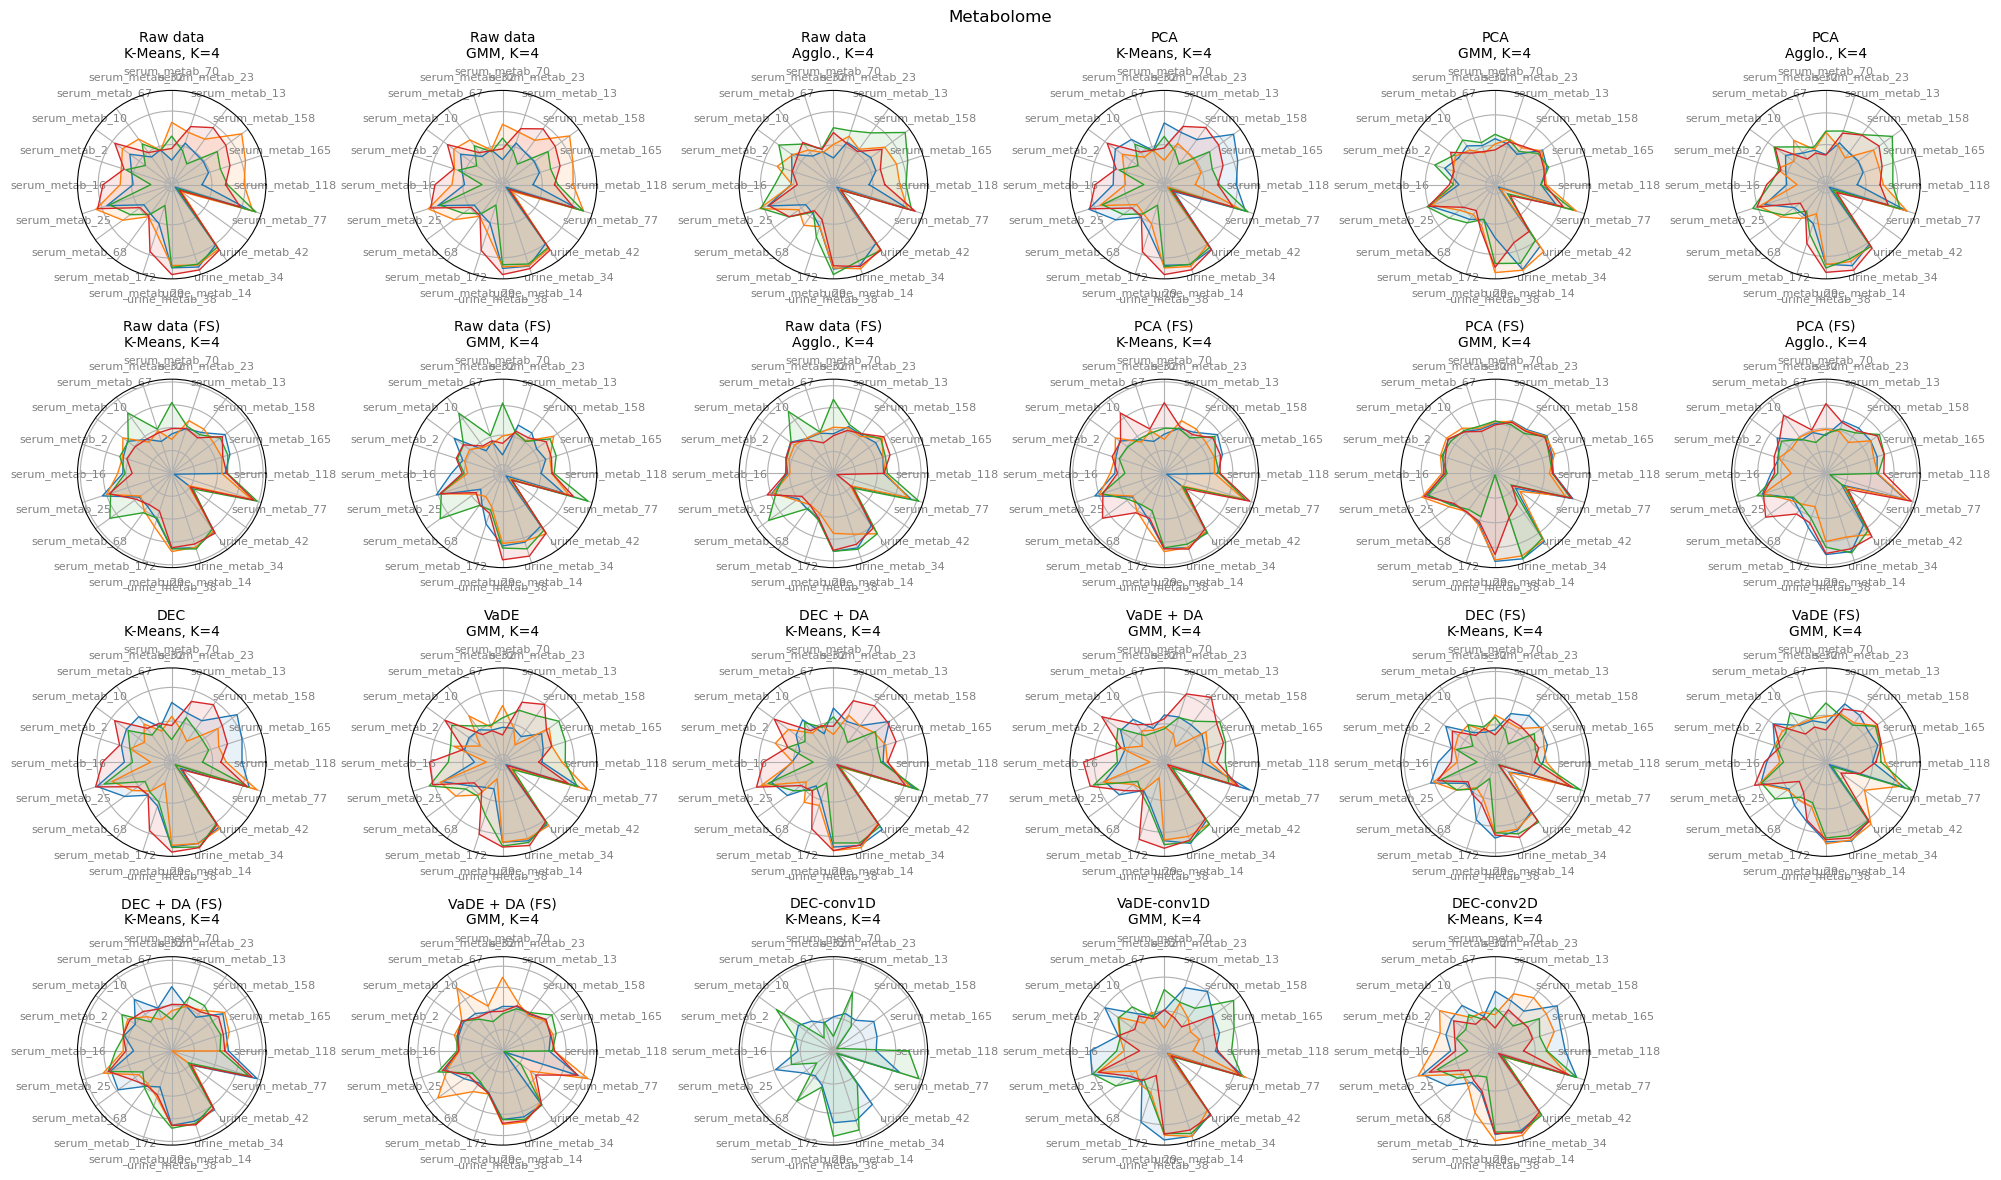
\includegraphics[width=\textwidth]{exposome_challenge/radialplots/metab_uncorr_mostvarfeat_k4.png}
                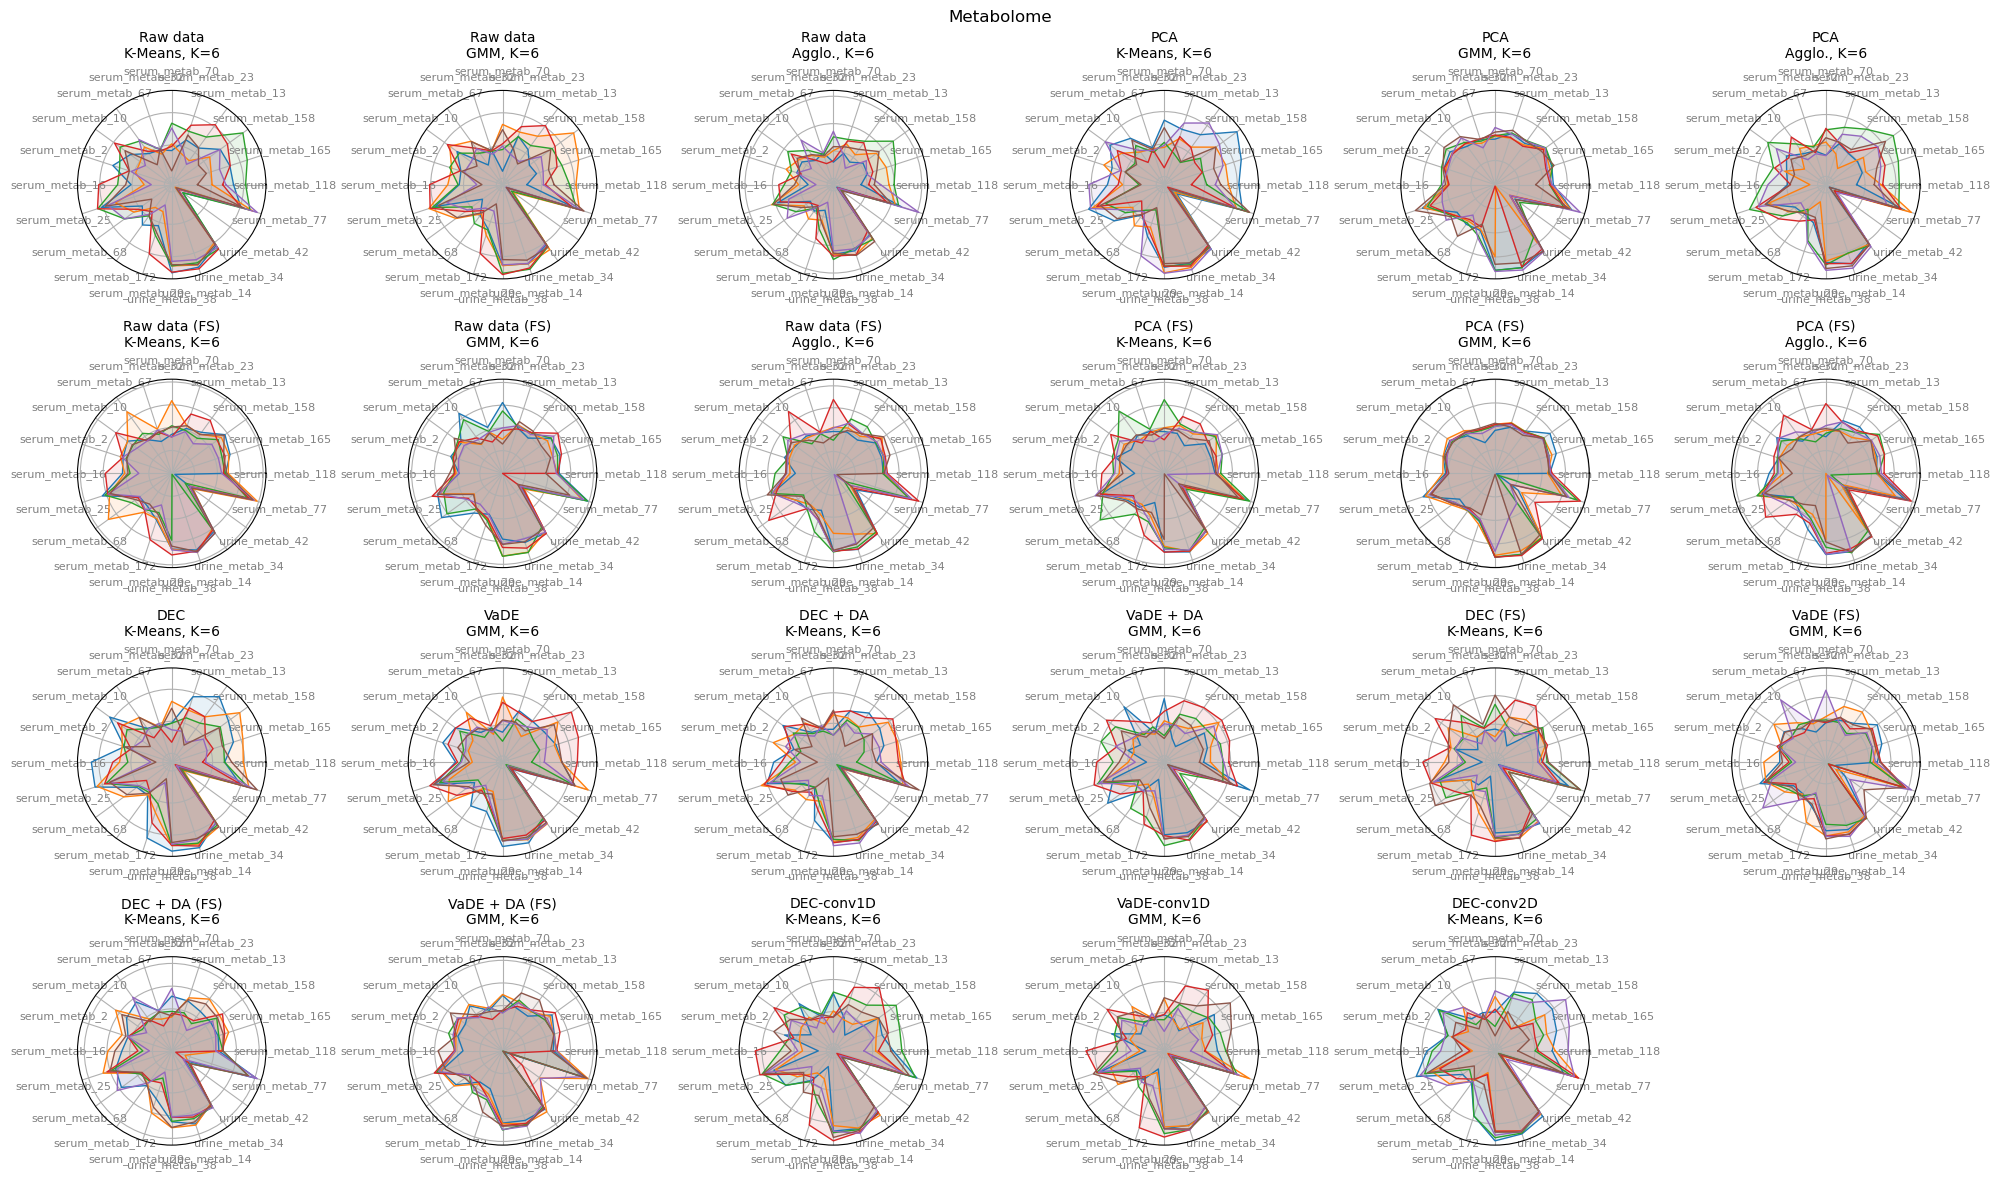
\includegraphics[width=\textwidth]{exposome_challenge/radialplots/metab_uncorr_mostvarfeat_k6.png}
                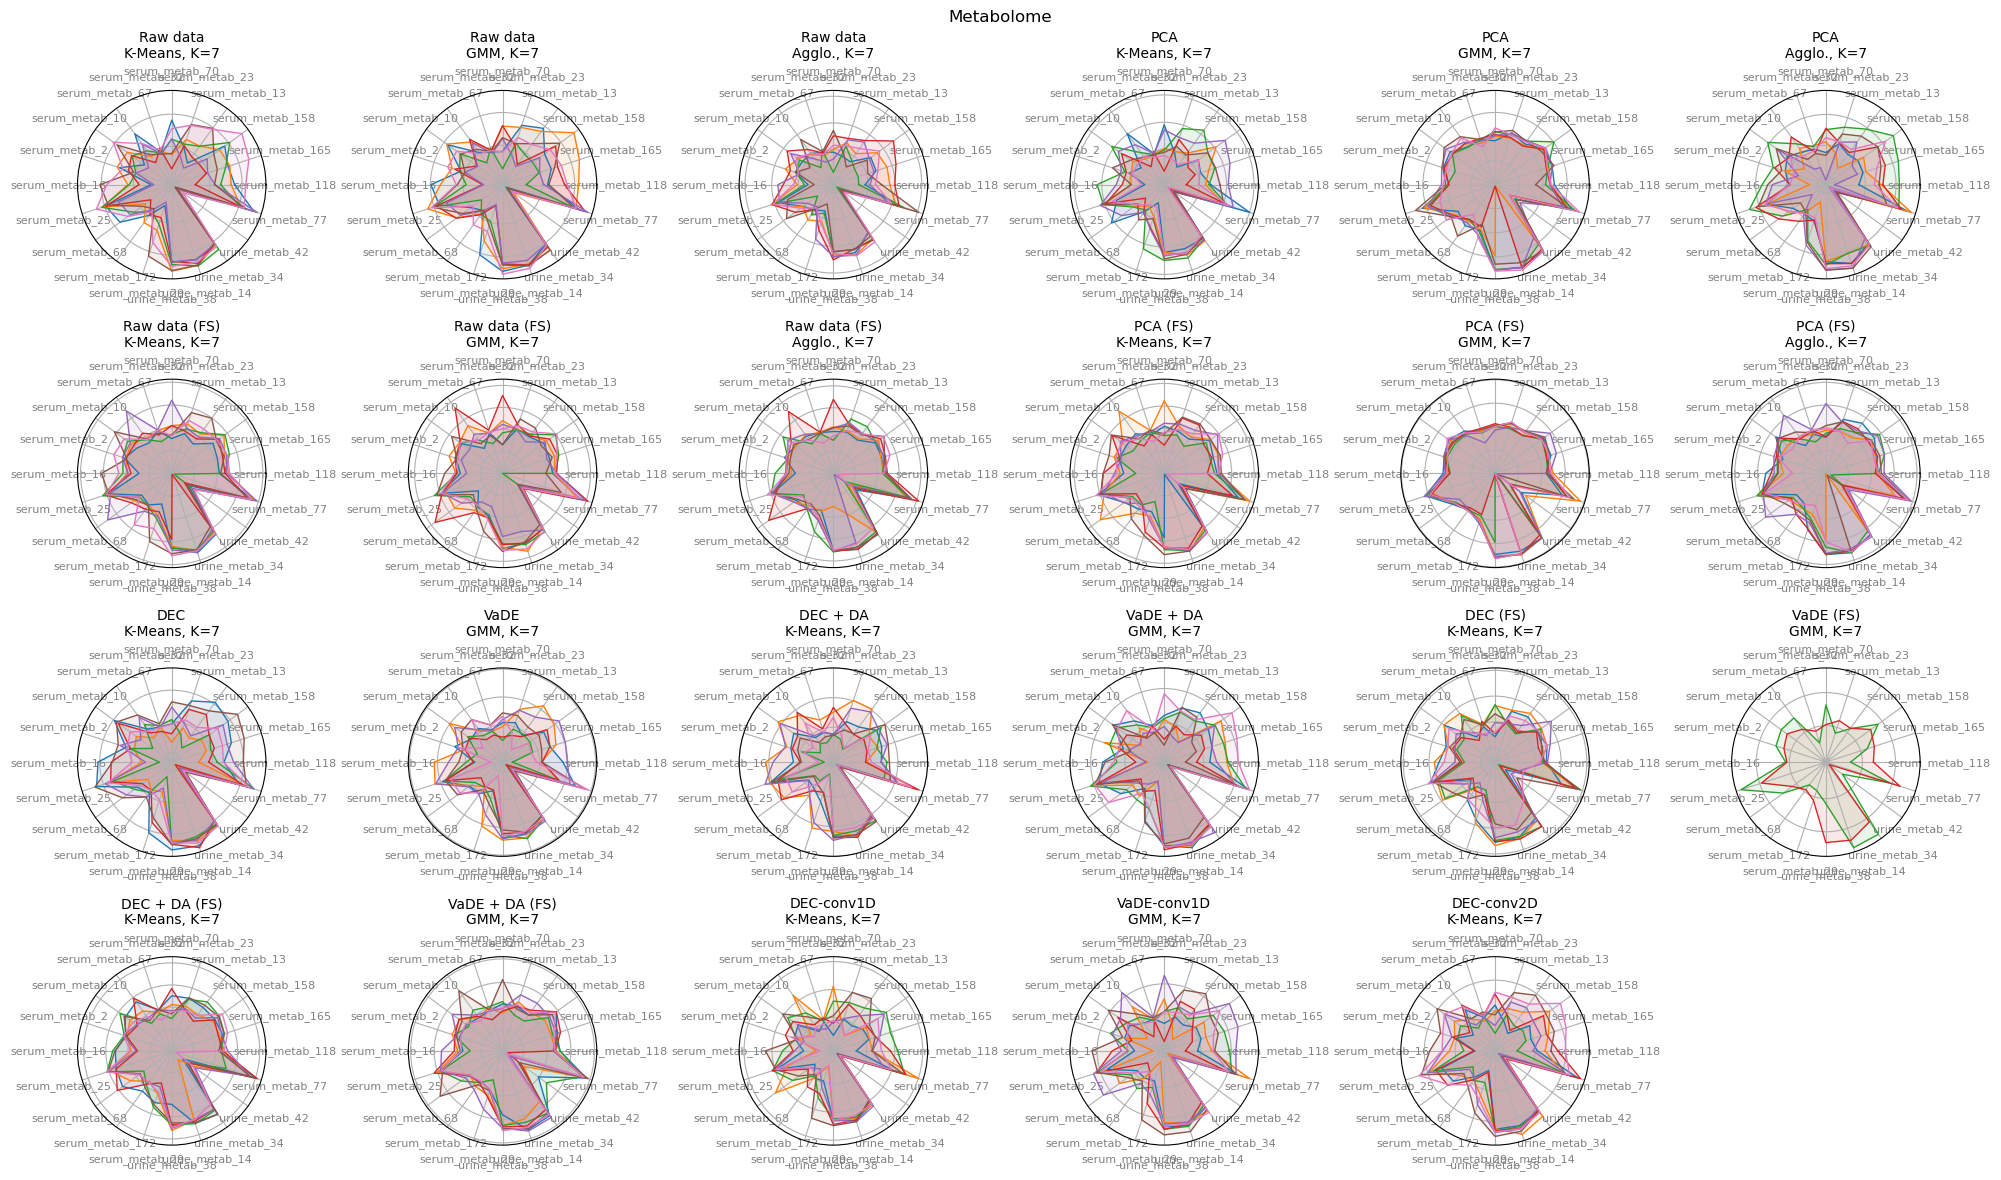
\includegraphics[width=\textwidth]{exposome_challenge/radialplots/metab_uncorr_mostvarfeat_k7.png}
            \end{center}

        \subsection{Conjunt de dades: metaboloma (corregit per l'efecte de log)}

            \paragraph{Dades fenotip:} distribució multivariant en funció dels clústers.

            \begin{center}
                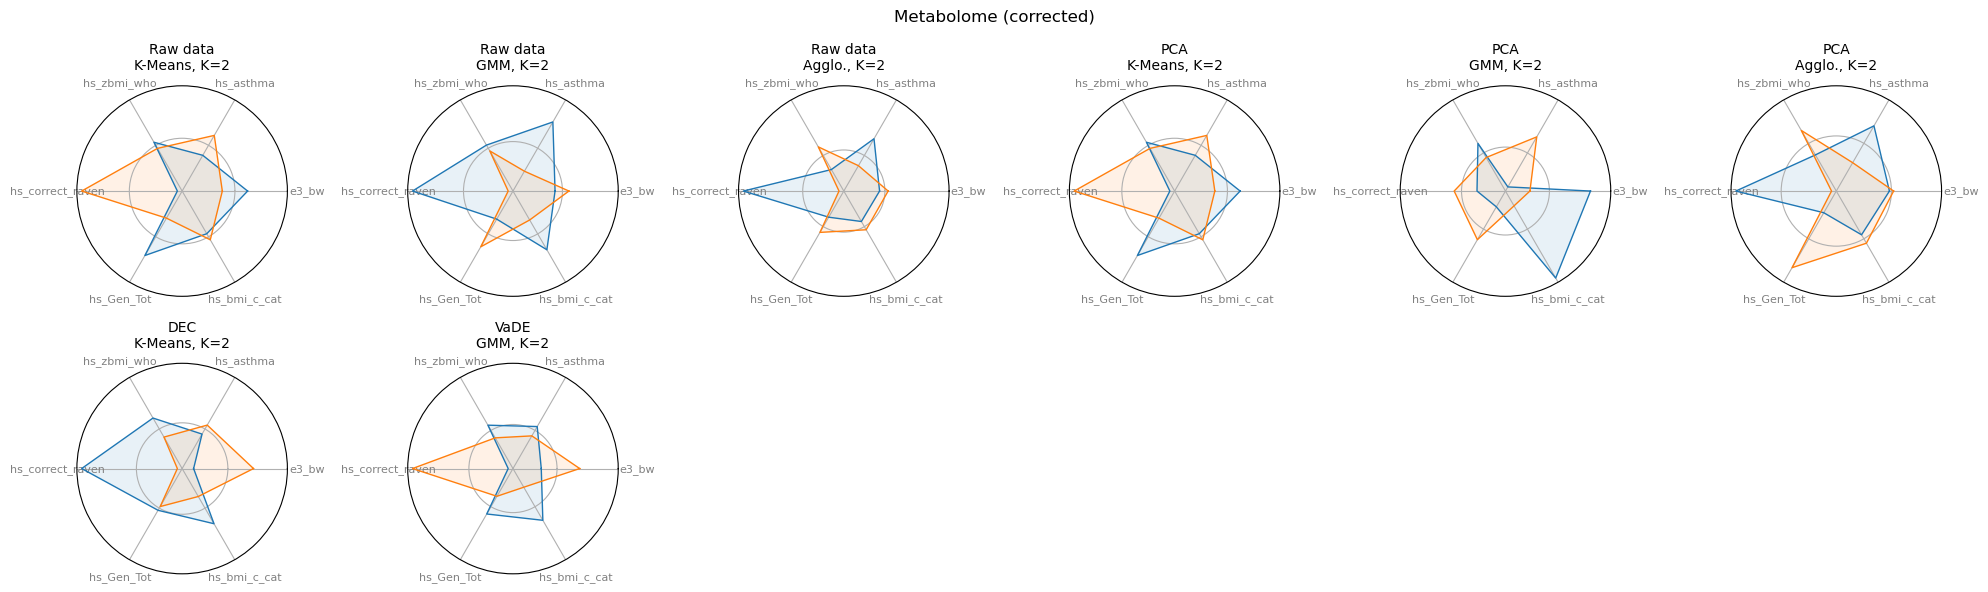
\includegraphics[width=\textwidth]{exposome_challenge/radialplots/metab_corr_feno_k2.png}
                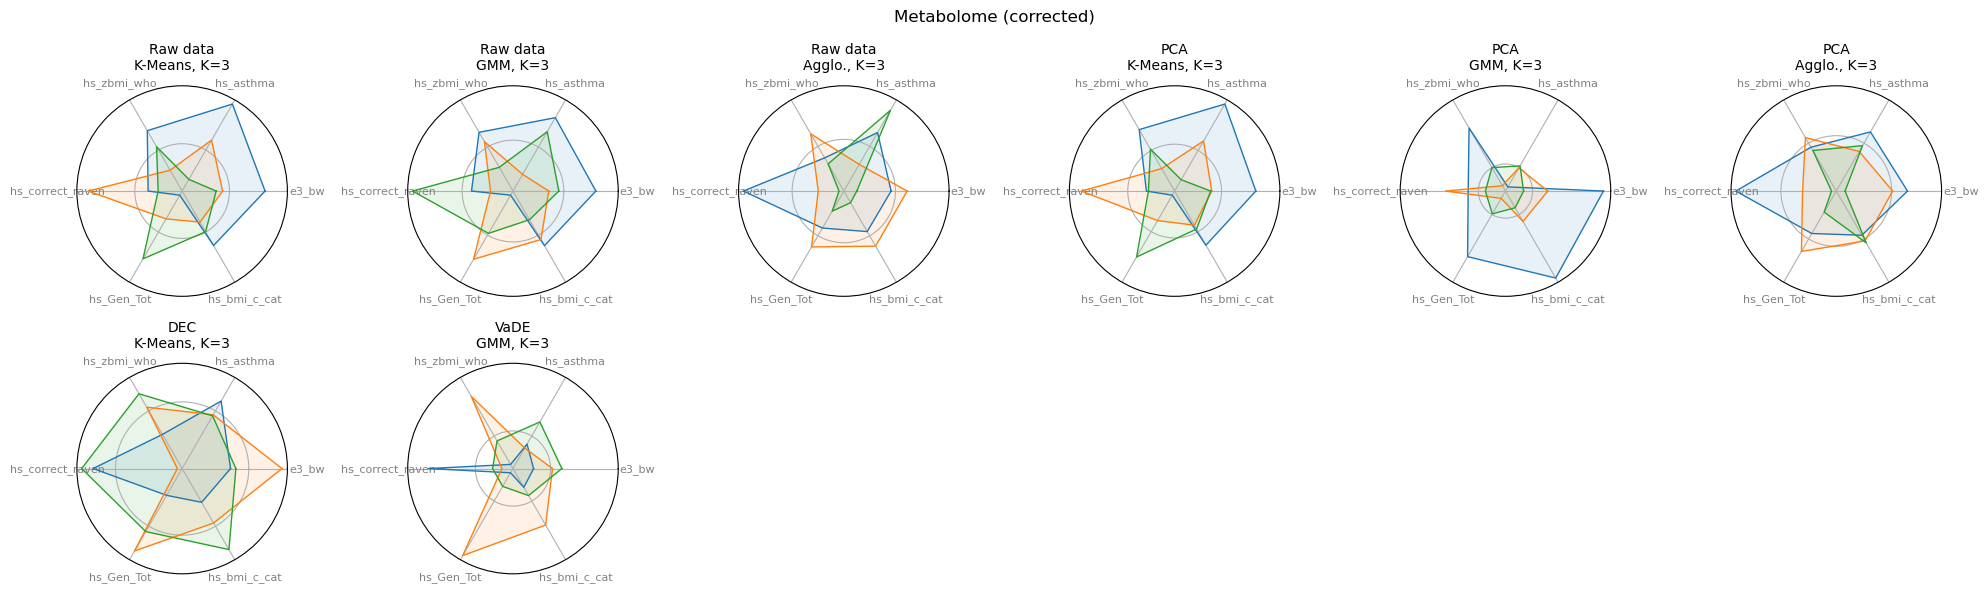
\includegraphics[width=\textwidth]{exposome_challenge/radialplots/metab_corr_feno_k3.png}
                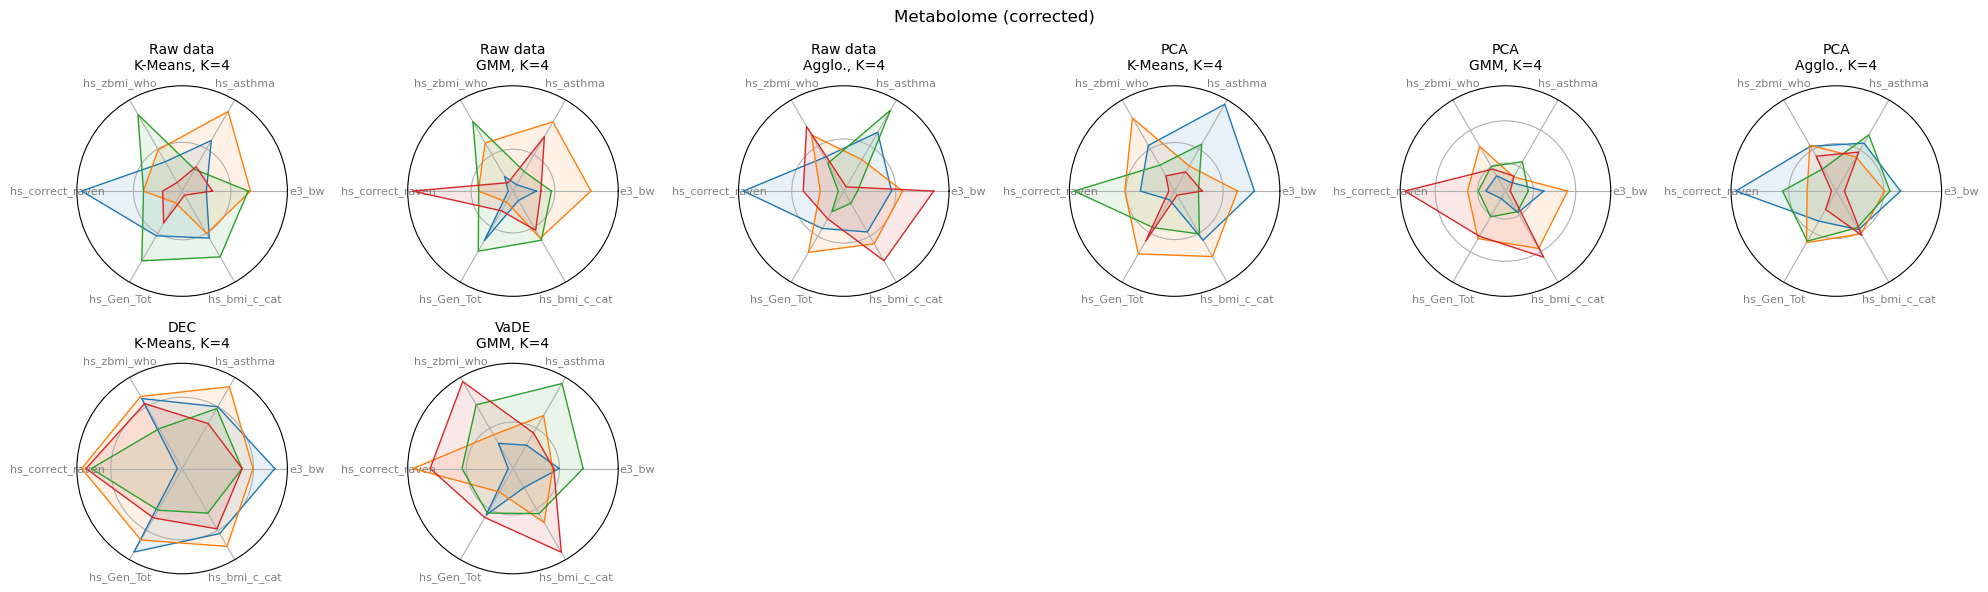
\includegraphics[width=\textwidth]{exposome_challenge/radialplots/metab_corr_feno_k4.png}
                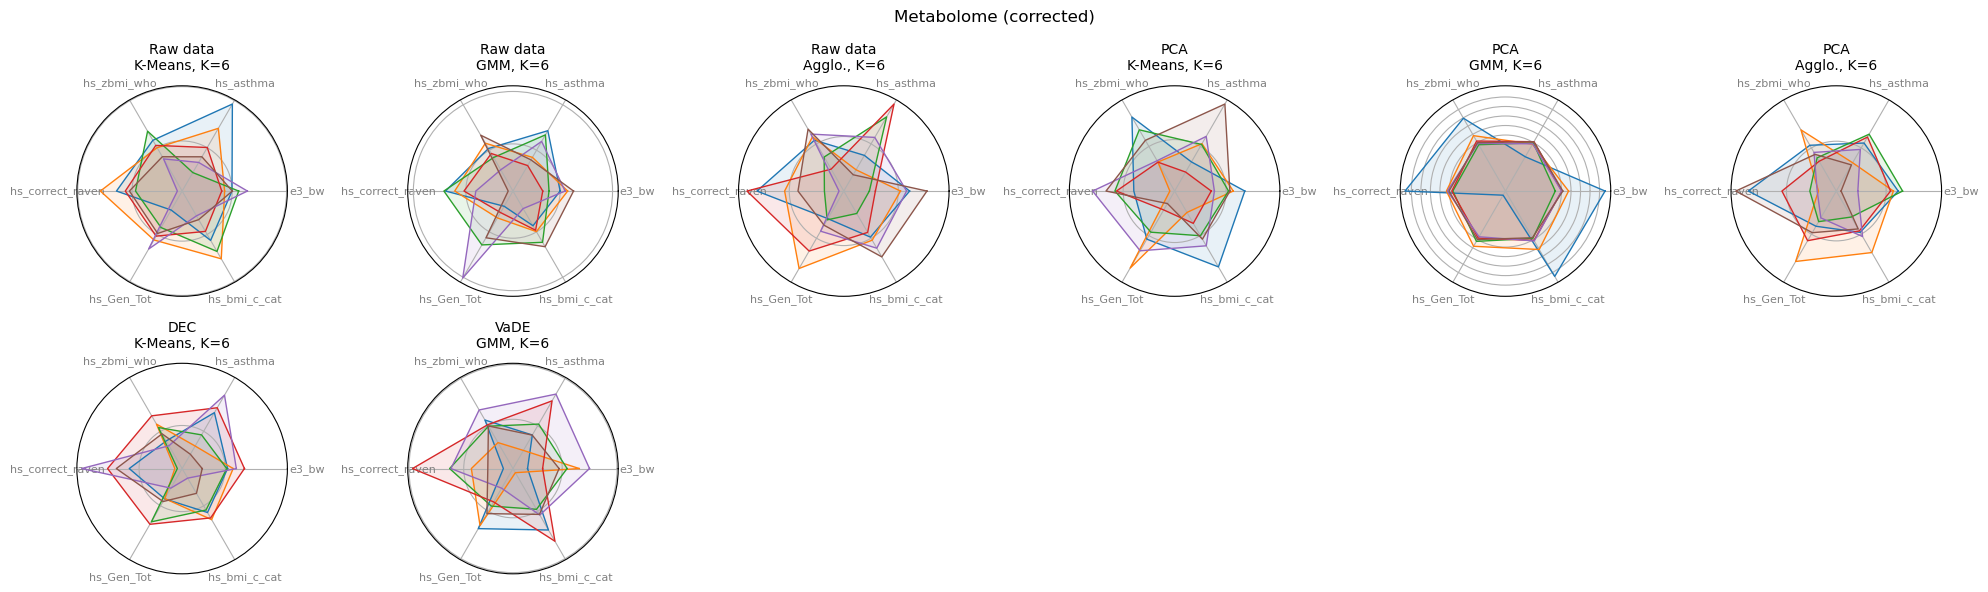
\includegraphics[width=\textwidth]{exposome_challenge/radialplots/metab_corr_feno_k6.png}
                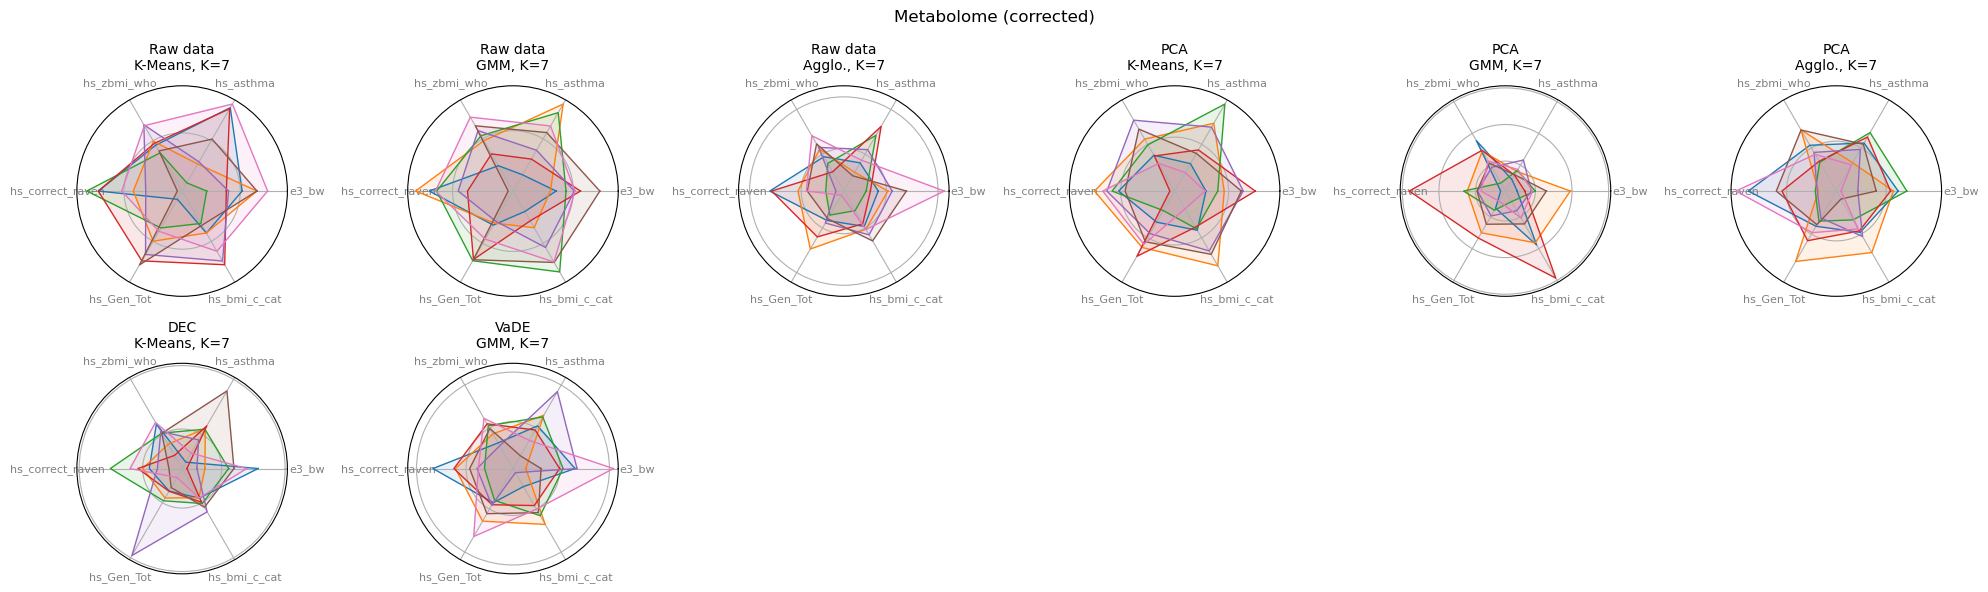
\includegraphics[width=\textwidth]{exposome_challenge/radialplots/metab_corr_feno_k7.png}
            \end{center}

            \paragraph{Dades covariables:} distribució multivariant en funció dels clústers.

            \begin{center}
                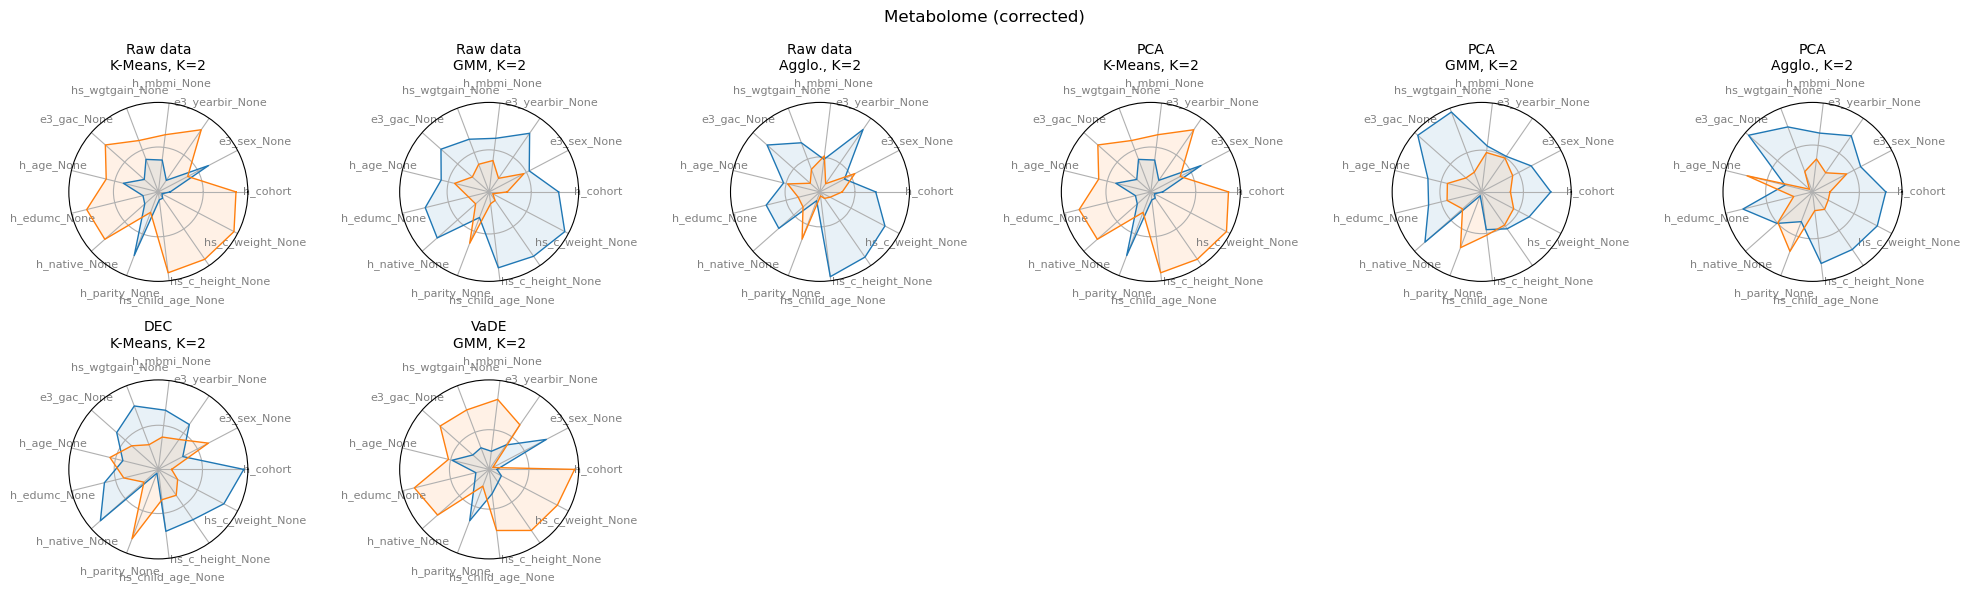
\includegraphics[width=\textwidth]{exposome_challenge/radialplots/metab_corr_covars_k2.png}
                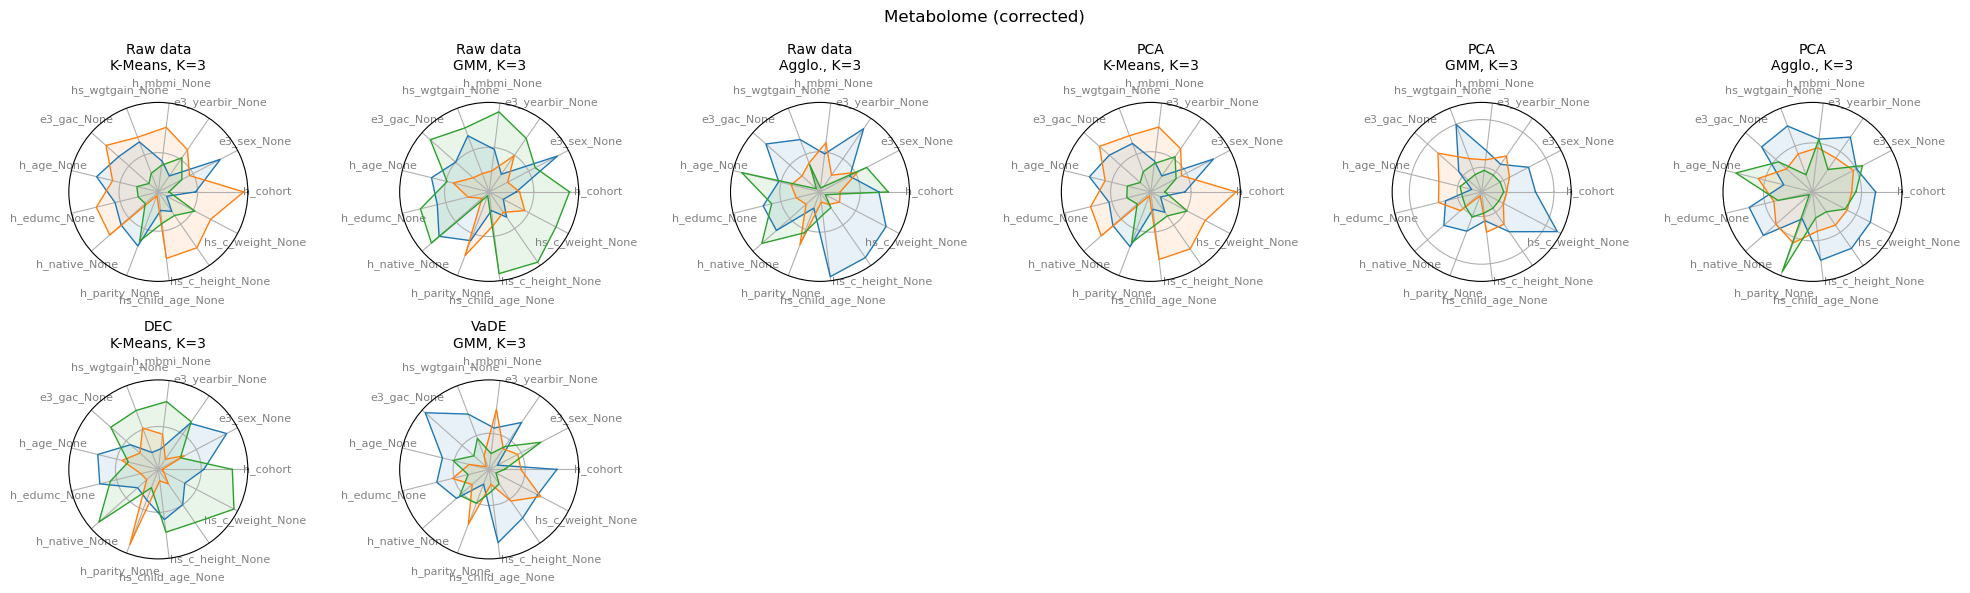
\includegraphics[width=\textwidth]{exposome_challenge/radialplots/metab_corr_covars_k3.png}
                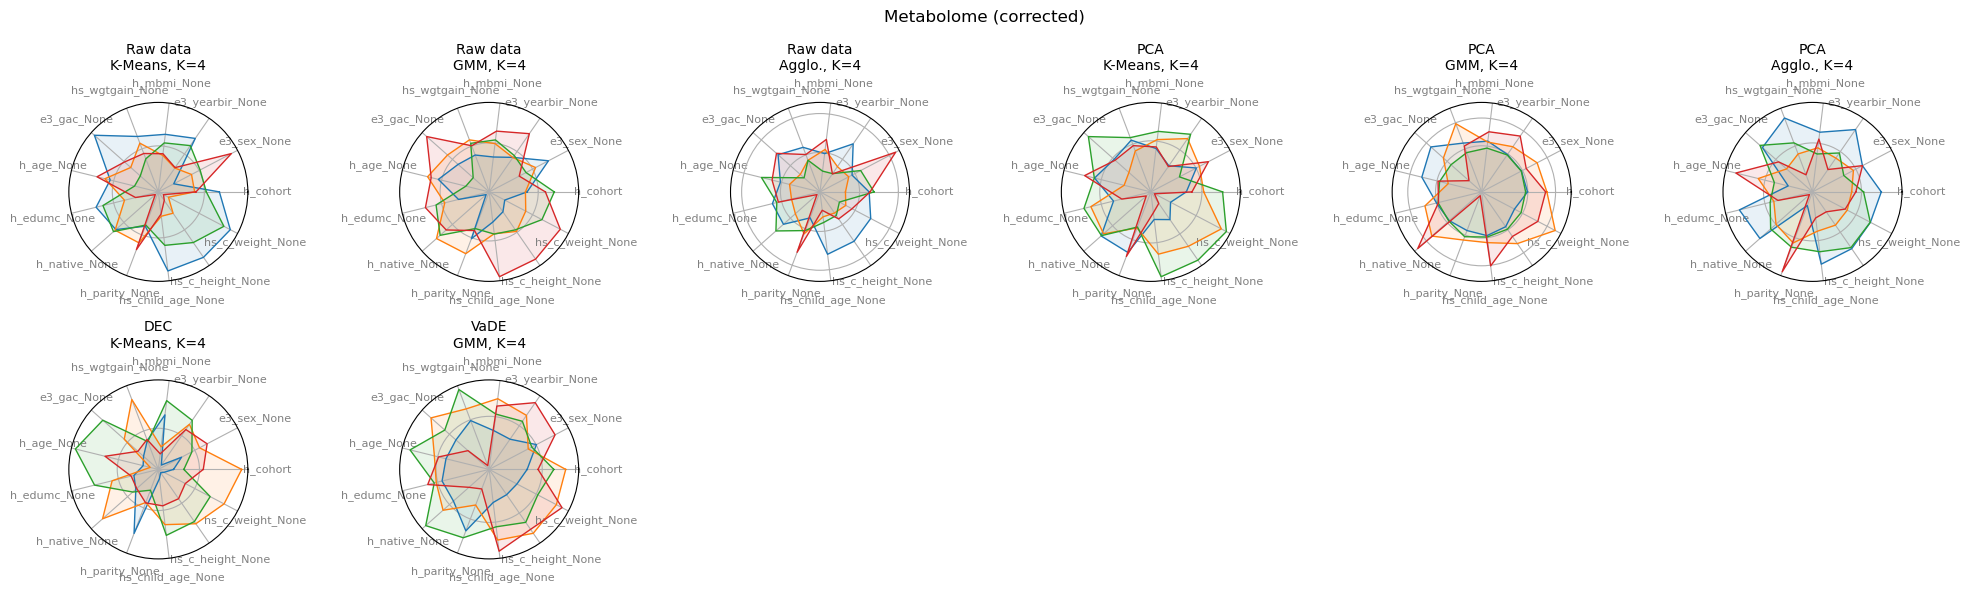
\includegraphics[width=\textwidth]{exposome_challenge/radialplots/metab_corr_covars_k4.png}
                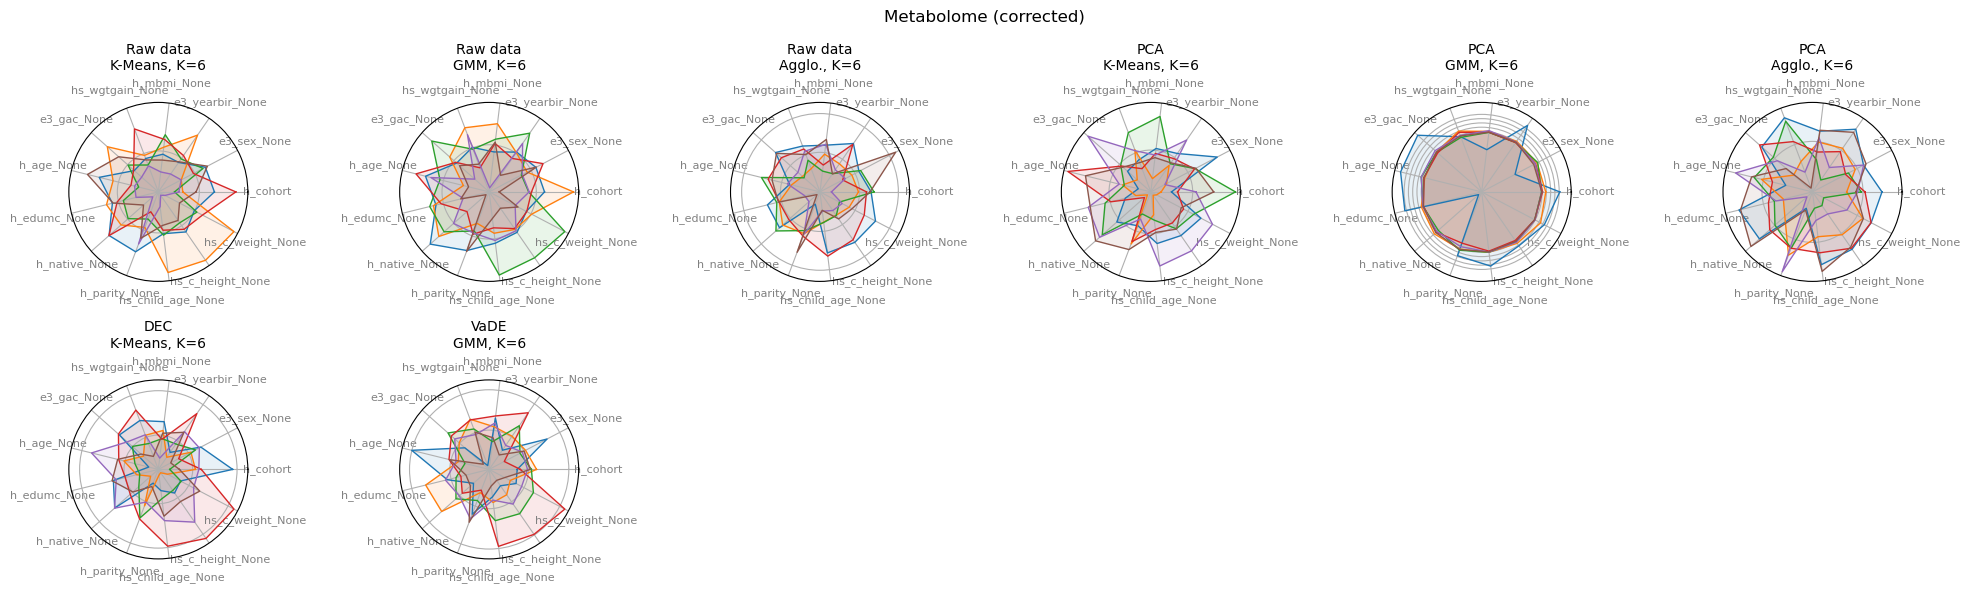
\includegraphics[width=\textwidth]{exposome_challenge/radialplots/metab_corr_covars_k6.png}
                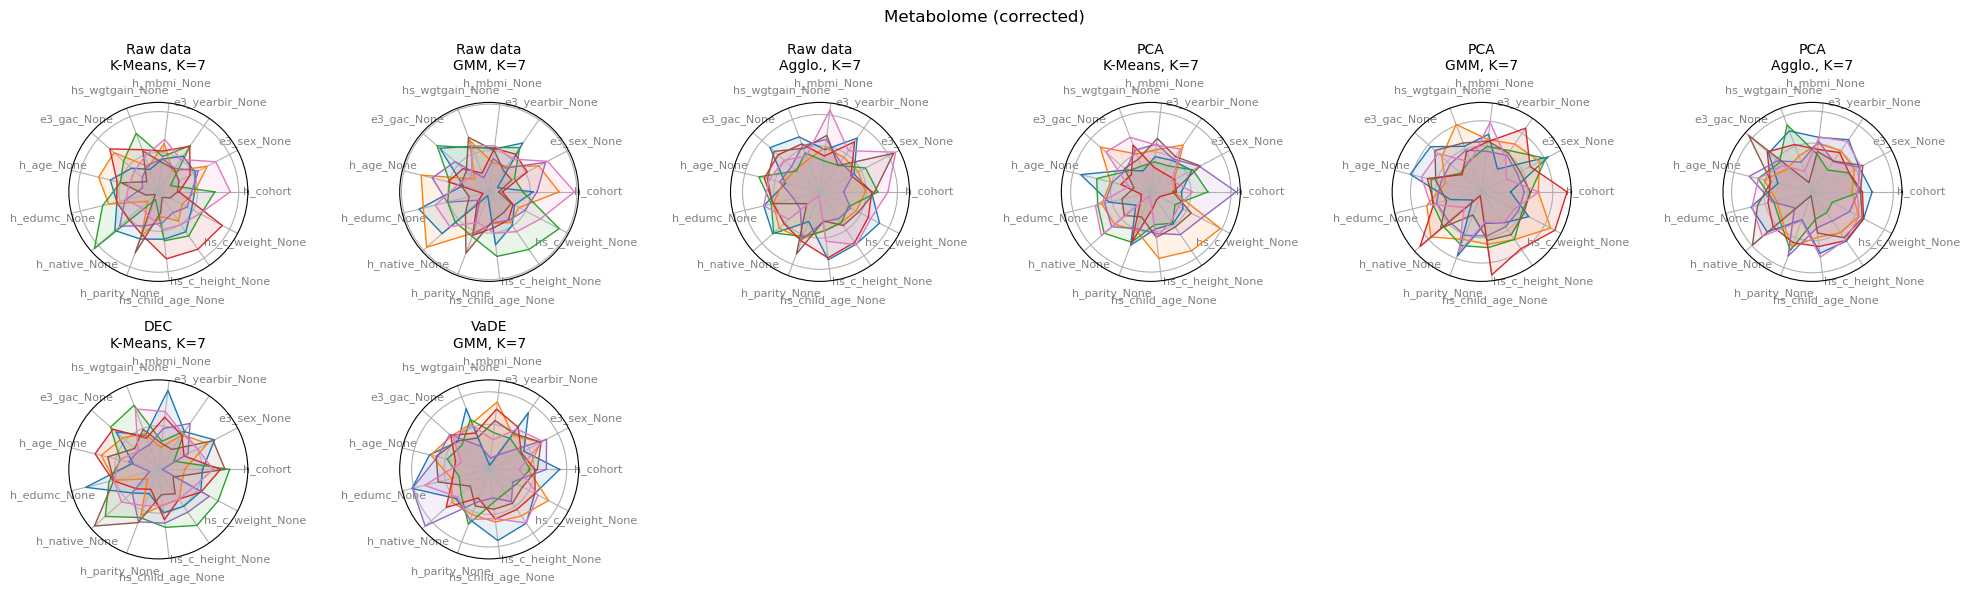
\includegraphics[width=\textwidth]{exposome_challenge/radialplots/metab_corr_covars_k7.png}
            \end{center}

            \paragraph{Dades metaboloma:} distribució multivariant en funció dels clústers (20 variables amb major variablitat).

            \begin{center}
                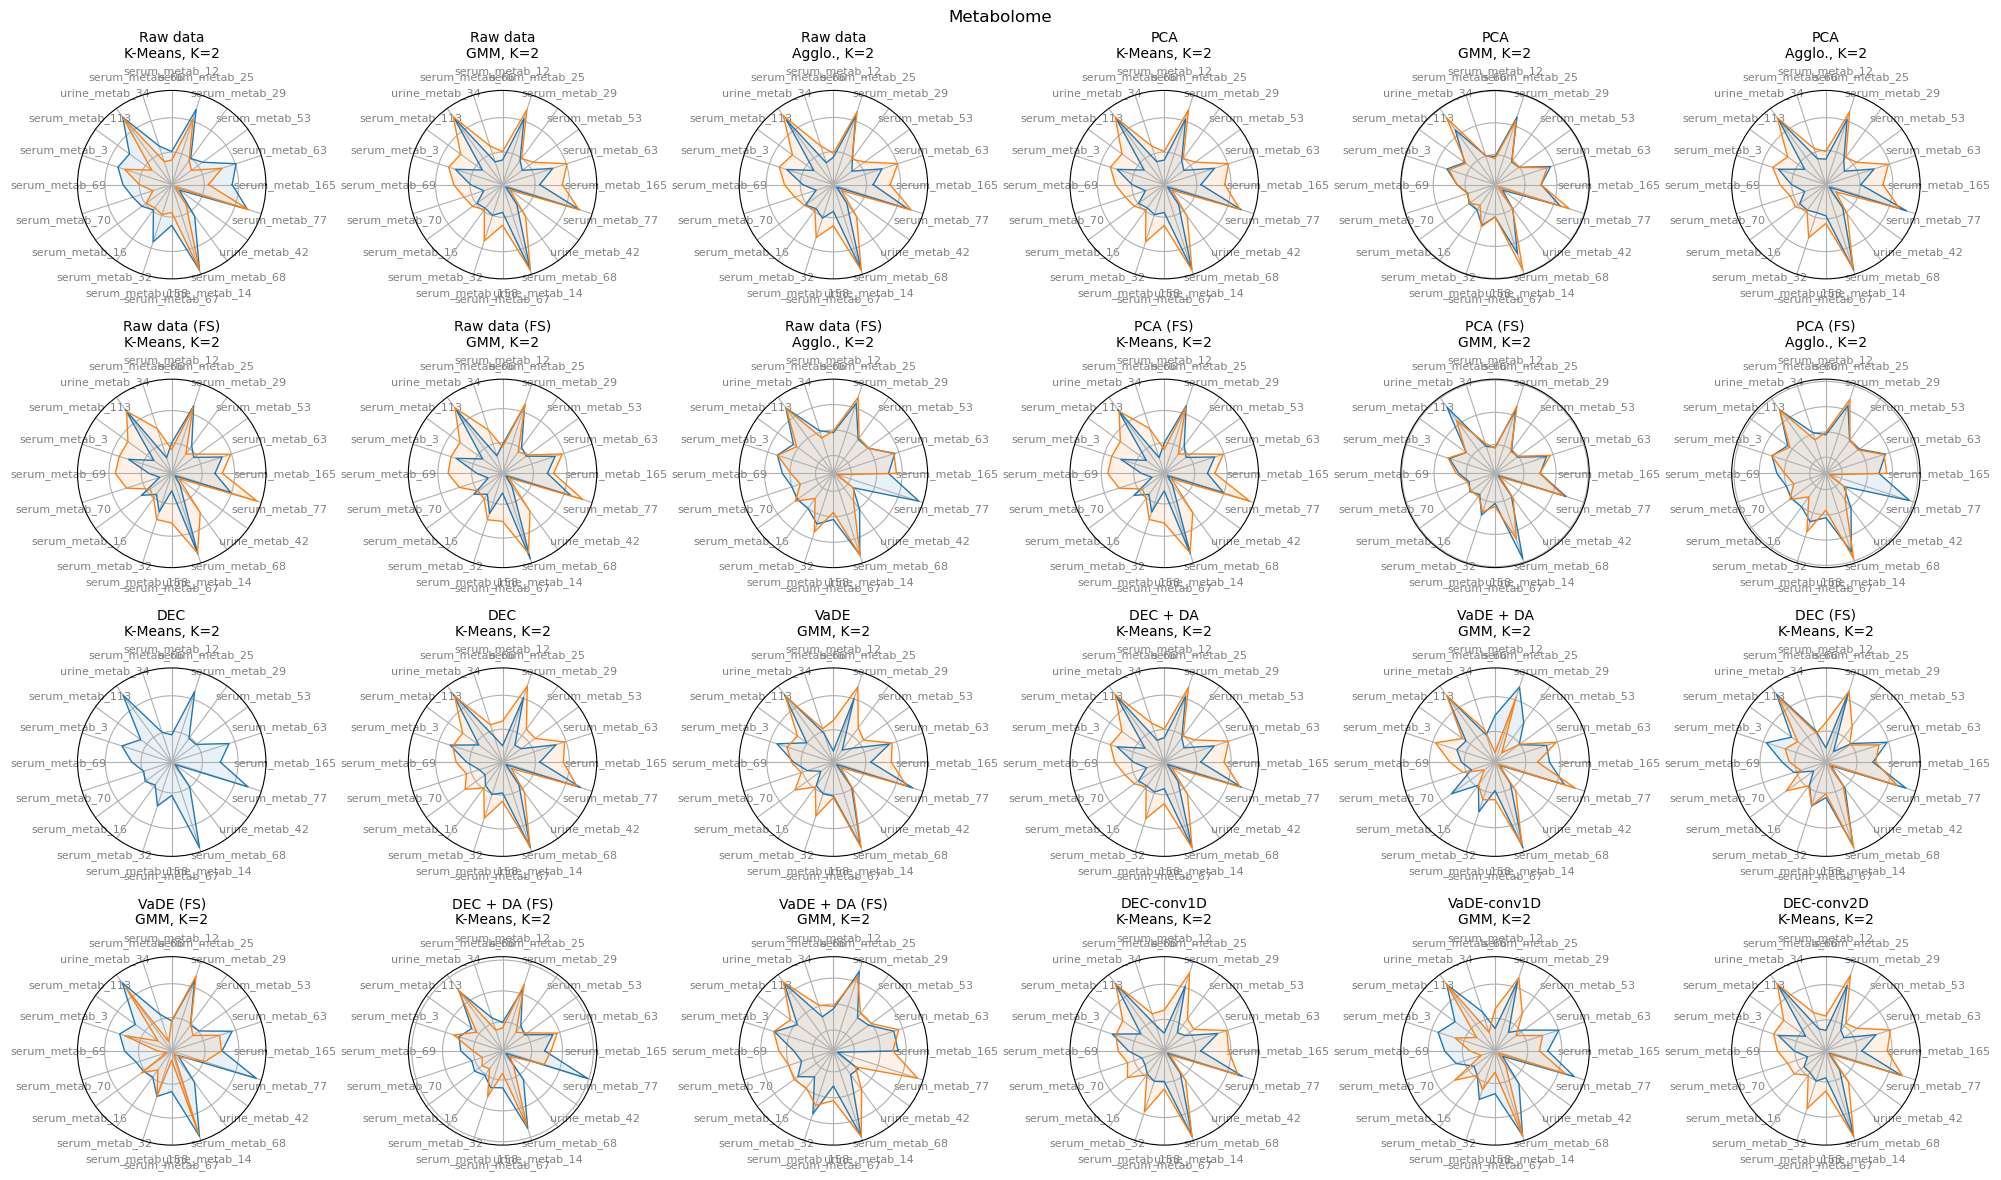
\includegraphics[width=\textwidth]{exposome_challenge/radialplots/metab_corr_mostvarfeat_k2.png}
                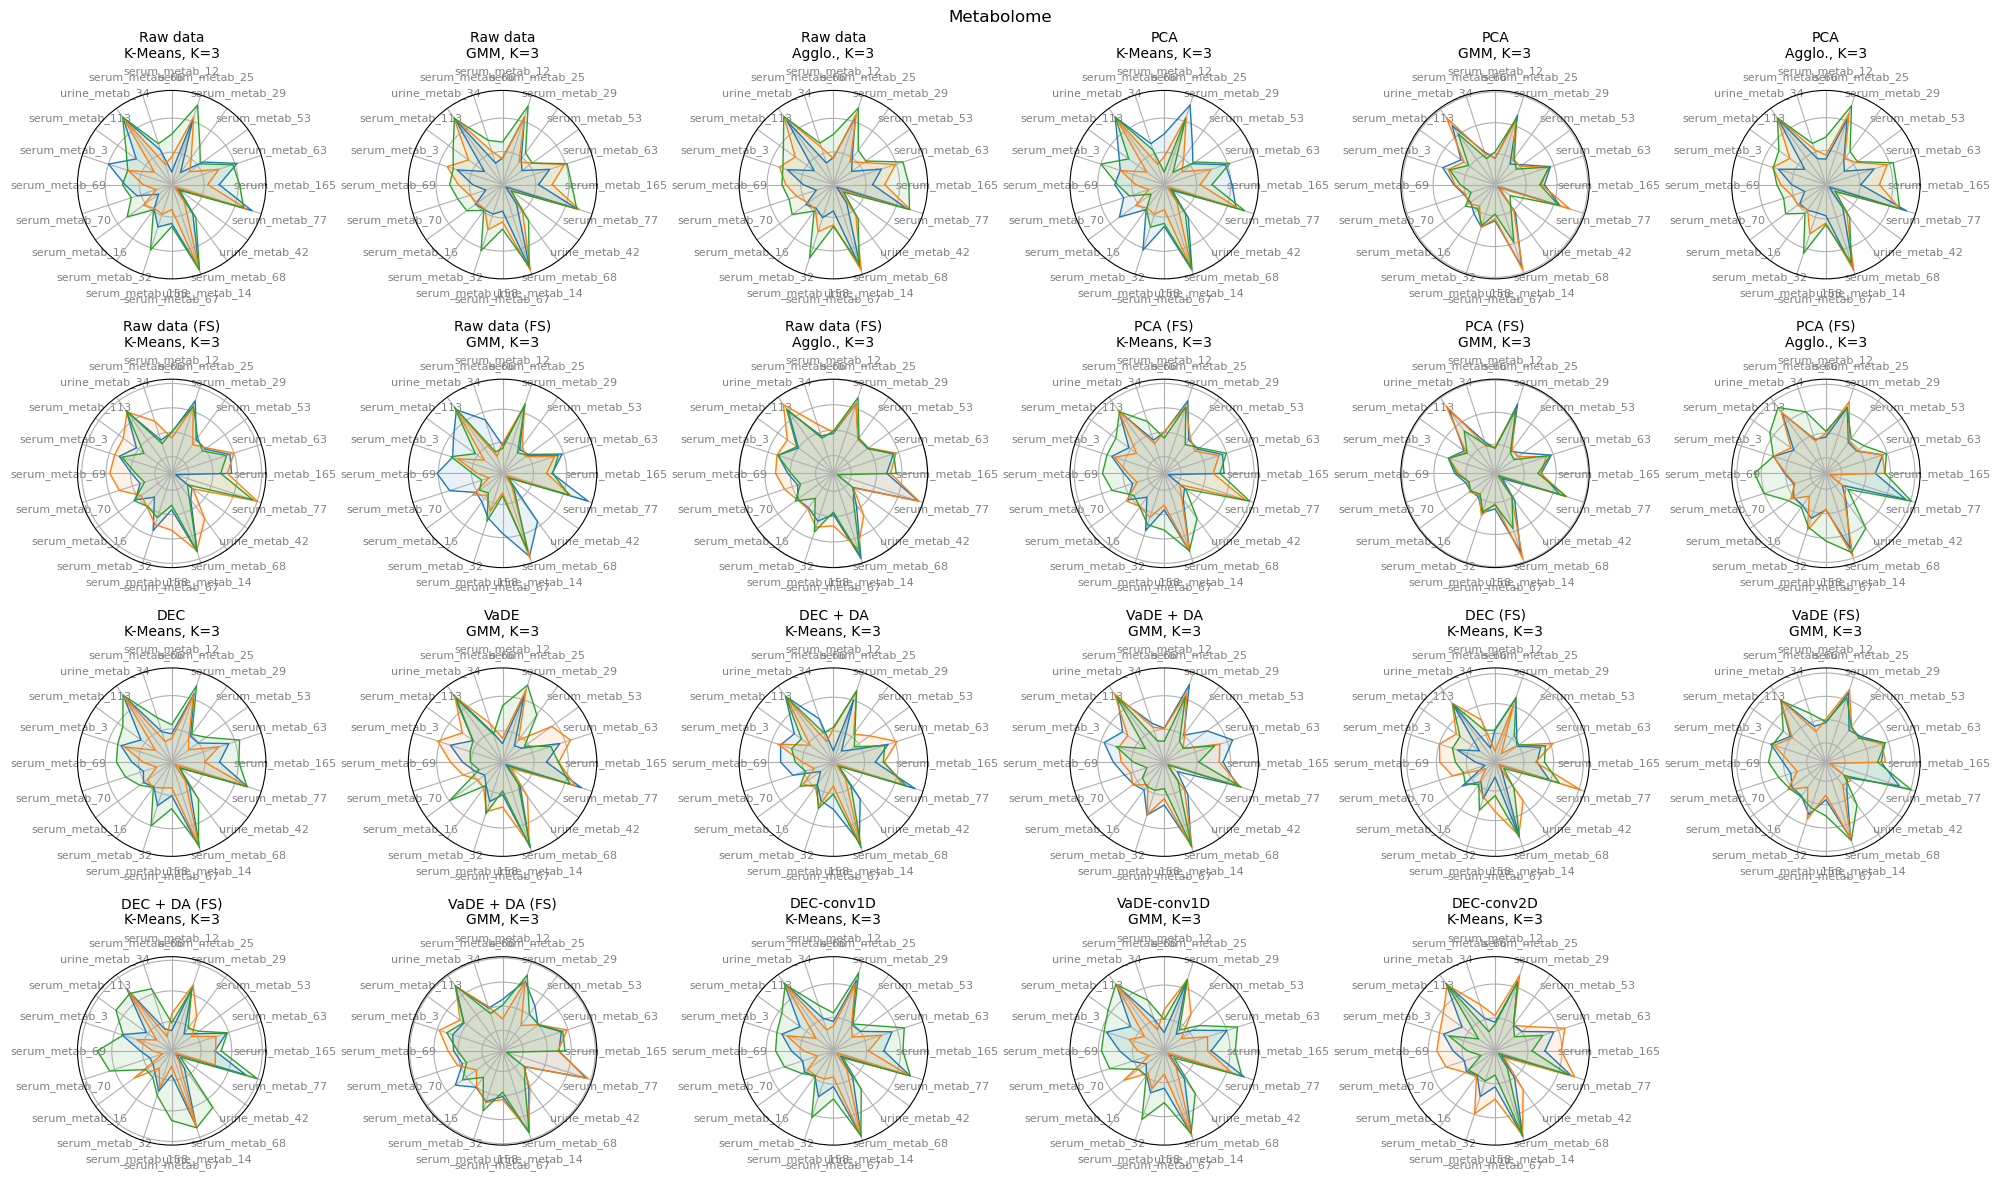
\includegraphics[width=\textwidth]{exposome_challenge/radialplots/metab_corr_mostvarfeat_k3.png}
                \includegraphics[width=\textwidth]{exposome_challenge/radialplots/metab_corr_mostvarfeat_k4.png}
                \includegraphics[width=\textwidth]{exposome_challenge/radialplots/metab_corr_mostvarfeat_k6.png}
                \includegraphics[width=\textwidth]{exposome_challenge/radialplots/metab_corr_mostvarfeat_k7.png}
            \end{center}

        \subsection{Conjunt de dades: exposoma}

            \paragraph{Dades fenotip:} distribució multivariant en funció dels clústers.

            \begin{center}
                \includegraphics[width=\textwidth]{exposome_challenge/radialplots/exposome_uncorr_feno_k2.png}
                \includegraphics[width=\textwidth]{exposome_challenge/radialplots/exposome_uncorr_feno_k3.png}
                \includegraphics[width=\textwidth]{exposome_challenge/radialplots/exposome_uncorr_feno_k4.png}
                \includegraphics[width=\textwidth]{exposome_challenge/radialplots/exposome_uncorr_feno_k6.png}
                \includegraphics[width=\textwidth]{exposome_challenge/radialplots/exposome_uncorr_feno_k7.png}
            \end{center}

            \paragraph{Dades covariables:} distribució multivariant en funció dels clústers.

            \begin{center}
                \includegraphics[width=\textwidth]{exposome_challenge/radialplots/exposome_uncorr_covars_k2.png}
                \includegraphics[width=\textwidth]{exposome_challenge/radialplots/exposome_uncorr_covars_k3.png}
                \includegraphics[width=\textwidth]{exposome_challenge/radialplots/exposome_uncorr_covars_k4.png}
                \includegraphics[width=\textwidth]{exposome_challenge/radialplots/exposome_uncorr_covars_k6.png}
                \includegraphics[width=\textwidth]{exposome_challenge/radialplots/exposome_uncorr_covars_k7.png}
            \end{center}

            \paragraph{Dades metaboloma:} distribució multivariant en funció dels clústers (20 variables amb major variablitat).

            \begin{center}
                \includegraphics[width=\textwidth]{exposome_challenge/radialplots/exposome_uncorr_mostvarfeat_k2.png}
                \includegraphics[width=\textwidth]{exposome_challenge/radialplots/exposome_uncorr_mostvarfeat_k3.png}
                \includegraphics[width=\textwidth]{exposome_challenge/radialplots/exposome_uncorr_mostvarfeat_k4.png}
                \includegraphics[width=\textwidth]{exposome_challenge/radialplots/exposome_uncorr_mostvarfeat_k6.png}
                \includegraphics[width=\textwidth]{exposome_challenge/radialplots/exposome_uncorr_mostvarfeat_k7.png}
            \end{center}

        \subsection{Conjunt de dades: exposoma (corregit per l'efecte de log)}

            \paragraph{Dades fenotip:} distribució multivariant en funció dels clústers.

            \begin{center}
                \includegraphics[width=\textwidth]{exposome_challenge/radialplots/exposome_corr_feno_k2.png}
                \includegraphics[width=\textwidth]{exposome_challenge/radialplots/exposome_corr_feno_k3.png}
                \includegraphics[width=\textwidth]{exposome_challenge/radialplots/exposome_corr_feno_k4.png}
                \includegraphics[width=\textwidth]{exposome_challenge/radialplots/exposome_corr_feno_k6.png}
                \includegraphics[width=\textwidth]{exposome_challenge/radialplots/exposome_corr_feno_k7.png}
            \end{center}

            \paragraph{Dades covariables:} distribució multivariant en funció dels clústers.

            \begin{center}
                \includegraphics[width=\textwidth]{exposome_challenge/radialplots/exposome_corr_covars_k2.png}
                \includegraphics[width=\textwidth]{exposome_challenge/radialplots/exposome_corr_covars_k3.png}
                \includegraphics[width=\textwidth]{exposome_challenge/radialplots/exposome_corr_covars_k4.png}
                \includegraphics[width=\textwidth]{exposome_challenge/radialplots/exposome_corr_covars_k6.png}
                \includegraphics[width=\textwidth]{exposome_challenge/radialplots/exposome_corr_covars_k7.png}
            \end{center}

            \paragraph{Dades metaboloma:} distribució multivariant en funció dels clústers (20 variables amb major variablitat).

            \begin{center}
                \includegraphics[width=\textwidth]{exposome_challenge/radialplots/exposome_corr_mostvarfeat_k2.png}
                \includegraphics[width=\textwidth]{exposome_challenge/radialplots/exposome_corr_mostvarfeat_k3.png}
                \includegraphics[width=\textwidth]{exposome_challenge/radialplots/exposome_corr_mostvarfeat_k4.png}
                \includegraphics[width=\textwidth]{exposome_challenge/radialplots/exposome_corr_mostvarfeat_k6.png}
                \includegraphics[width=\textwidth]{exposome_challenge/radialplots/exposome_corr_mostvarfeat_k7.png}
            \end{center}






\end{document}
